% Options for packages loaded elsewhere
\PassOptionsToPackage{unicode}{hyperref}
\PassOptionsToPackage{hyphens}{url}
%
\documentclass[
]{book}
\usepackage{lmodern}
\usepackage{amssymb,amsmath}
\usepackage{ifxetex,ifluatex}
\ifnum 0\ifxetex 1\fi\ifluatex 1\fi=0 % if pdftex
  \usepackage[T1]{fontenc}
  \usepackage[utf8]{inputenc}
  \usepackage{textcomp} % provide euro and other symbols
\else % if luatex or xetex
  \usepackage{unicode-math}
  \defaultfontfeatures{Scale=MatchLowercase}
  \defaultfontfeatures[\rmfamily]{Ligatures=TeX,Scale=1}
\fi
% Use upquote if available, for straight quotes in verbatim environments
\IfFileExists{upquote.sty}{\usepackage{upquote}}{}
\IfFileExists{microtype.sty}{% use microtype if available
  \usepackage[]{microtype}
  \UseMicrotypeSet[protrusion]{basicmath} % disable protrusion for tt fonts
}{}
\makeatletter
\@ifundefined{KOMAClassName}{% if non-KOMA class
  \IfFileExists{parskip.sty}{%
    \usepackage{parskip}
  }{% else
    \setlength{\parindent}{0pt}
    \setlength{\parskip}{6pt plus 2pt minus 1pt}}
}{% if KOMA class
  \KOMAoptions{parskip=half}}
\makeatother
\usepackage{xcolor}
\IfFileExists{xurl.sty}{\usepackage{xurl}}{} % add URL line breaks if available
\IfFileExists{bookmark.sty}{\usepackage{bookmark}}{\usepackage{hyperref}}
\hypersetup{
  pdftitle={The guts of the dispRity package},
  pdfauthor={Thomas Guillerme (guillert@tcd.ie)},
  hidelinks,
  pdfcreator={LaTeX via pandoc}}
\urlstyle{same} % disable monospaced font for URLs
\usepackage{color}
\usepackage{fancyvrb}
\newcommand{\VerbBar}{|}
\newcommand{\VERB}{\Verb[commandchars=\\\{\}]}
\DefineVerbatimEnvironment{Highlighting}{Verbatim}{commandchars=\\\{\}}
% Add ',fontsize=\small' for more characters per line
\usepackage{framed}
\definecolor{shadecolor}{RGB}{248,248,248}
\newenvironment{Shaded}{\begin{snugshade}}{\end{snugshade}}
\newcommand{\AlertTok}[1]{\textcolor[rgb]{0.94,0.16,0.16}{#1}}
\newcommand{\AnnotationTok}[1]{\textcolor[rgb]{0.56,0.35,0.01}{\textbf{\textit{#1}}}}
\newcommand{\AttributeTok}[1]{\textcolor[rgb]{0.77,0.63,0.00}{#1}}
\newcommand{\BaseNTok}[1]{\textcolor[rgb]{0.00,0.00,0.81}{#1}}
\newcommand{\BuiltInTok}[1]{#1}
\newcommand{\CharTok}[1]{\textcolor[rgb]{0.31,0.60,0.02}{#1}}
\newcommand{\CommentTok}[1]{\textcolor[rgb]{0.56,0.35,0.01}{\textit{#1}}}
\newcommand{\CommentVarTok}[1]{\textcolor[rgb]{0.56,0.35,0.01}{\textbf{\textit{#1}}}}
\newcommand{\ConstantTok}[1]{\textcolor[rgb]{0.00,0.00,0.00}{#1}}
\newcommand{\ControlFlowTok}[1]{\textcolor[rgb]{0.13,0.29,0.53}{\textbf{#1}}}
\newcommand{\DataTypeTok}[1]{\textcolor[rgb]{0.13,0.29,0.53}{#1}}
\newcommand{\DecValTok}[1]{\textcolor[rgb]{0.00,0.00,0.81}{#1}}
\newcommand{\DocumentationTok}[1]{\textcolor[rgb]{0.56,0.35,0.01}{\textbf{\textit{#1}}}}
\newcommand{\ErrorTok}[1]{\textcolor[rgb]{0.64,0.00,0.00}{\textbf{#1}}}
\newcommand{\ExtensionTok}[1]{#1}
\newcommand{\FloatTok}[1]{\textcolor[rgb]{0.00,0.00,0.81}{#1}}
\newcommand{\FunctionTok}[1]{\textcolor[rgb]{0.00,0.00,0.00}{#1}}
\newcommand{\ImportTok}[1]{#1}
\newcommand{\InformationTok}[1]{\textcolor[rgb]{0.56,0.35,0.01}{\textbf{\textit{#1}}}}
\newcommand{\KeywordTok}[1]{\textcolor[rgb]{0.13,0.29,0.53}{\textbf{#1}}}
\newcommand{\NormalTok}[1]{#1}
\newcommand{\OperatorTok}[1]{\textcolor[rgb]{0.81,0.36,0.00}{\textbf{#1}}}
\newcommand{\OtherTok}[1]{\textcolor[rgb]{0.56,0.35,0.01}{#1}}
\newcommand{\PreprocessorTok}[1]{\textcolor[rgb]{0.56,0.35,0.01}{\textit{#1}}}
\newcommand{\RegionMarkerTok}[1]{#1}
\newcommand{\SpecialCharTok}[1]{\textcolor[rgb]{0.00,0.00,0.00}{#1}}
\newcommand{\SpecialStringTok}[1]{\textcolor[rgb]{0.31,0.60,0.02}{#1}}
\newcommand{\StringTok}[1]{\textcolor[rgb]{0.31,0.60,0.02}{#1}}
\newcommand{\VariableTok}[1]{\textcolor[rgb]{0.00,0.00,0.00}{#1}}
\newcommand{\VerbatimStringTok}[1]{\textcolor[rgb]{0.31,0.60,0.02}{#1}}
\newcommand{\WarningTok}[1]{\textcolor[rgb]{0.56,0.35,0.01}{\textbf{\textit{#1}}}}
\usepackage{longtable,booktabs}
% Correct order of tables after \paragraph or \subparagraph
\usepackage{etoolbox}
\makeatletter
\patchcmd\longtable{\par}{\if@noskipsec\mbox{}\fi\par}{}{}
\makeatother
% Allow footnotes in longtable head/foot
\IfFileExists{footnotehyper.sty}{\usepackage{footnotehyper}}{\usepackage{footnote}}
\makesavenoteenv{longtable}
\usepackage{graphicx}
\makeatletter
\def\maxwidth{\ifdim\Gin@nat@width>\linewidth\linewidth\else\Gin@nat@width\fi}
\def\maxheight{\ifdim\Gin@nat@height>\textheight\textheight\else\Gin@nat@height\fi}
\makeatother
% Scale images if necessary, so that they will not overflow the page
% margins by default, and it is still possible to overwrite the defaults
% using explicit options in \includegraphics[width, height, ...]{}
\setkeys{Gin}{width=\maxwidth,height=\maxheight,keepaspectratio}
% Set default figure placement to htbp
\makeatletter
\def\fps@figure{htbp}
\makeatother
\setlength{\emergencystretch}{3em} % prevent overfull lines
\providecommand{\tightlist}{%
  \setlength{\itemsep}{0pt}\setlength{\parskip}{0pt}}
\setcounter{secnumdepth}{5}
\usepackage{booktabs}
\usepackage[]{natbib}
\bibliographystyle{plainnat}

\title{The guts of the dispRity package}
\author{Thomas Guillerme (\href{mailto:guillert@tcd.ie}{\nolinkurl{guillert@tcd.ie}})}
\date{2022-08-09}

\begin{document}
\maketitle

{
\setcounter{tocdepth}{1}
\tableofcontents
}
\hypertarget{disprity}{%
\chapter{\texorpdfstring{\texttt{dispRity}}{dispRity}}\label{disprity}}

This is a package for measuring disparity (aka multidimensional space occupancy) in \texttt{R}.
It allows users to summarise matrices as representations as multidimensional spaces into a single value or distribution describing a specific aspect of this multidimensional space (the disparity).
Multidimensional spaces can be ordinated matrices from MDS, PCA, PCO, PCoA but the package is \emph{not} restricted to any type of matrices!
This manual is based on the version 1.7.

\hypertarget{what-is-disprity}{%
\section{\texorpdfstring{What is \texttt{dispRity}?}{What is dispRity?}}\label{what-is-disprity}}

This is a modular package for measuring disparity in \texttt{R}.
It allows users to summarise ordinated matrices (e.g.~MDS, PCA, PCO, PCoA) to perform some multidimensional analysis.
Typically, these analysis are used in palaeobiology and evolutionary biology to study the changes in morphology through time.
However, there are many more applications in ecology, evolution and beyond.

\hypertarget{modular}{%
\subsection{Modular?}\label{modular}}

Because their exist a multitude of ways to measure disparity, each adapted to every specific question, this package uses an easy to modify modular architecture.
In coding, each module is simply a function or a modification of a function that can be passed to the main functions of the package to tweak it to your proper needs!
In practice, you will notice throughout this manual that some function can take other functions as arguments: the modular architecture of this package allows you to use any function for these arguments (with some restrictions explained for each specific cases).
This will allow you to finely tune your multidimensional analysis to the needs of your specific question!

\hypertarget{installing-and-running-the-package}{%
\section{Installing and running the package}\label{installing-and-running-the-package}}

You can install this package easily, directly from the CRAN:

\begin{Shaded}
\begin{Highlighting}[]
\KeywordTok{install.packages}\NormalTok{(}\StringTok{"dispRity"}\NormalTok{)}
\end{Highlighting}
\end{Shaded}

Alternatively, for the most up to data version and some functionalities not compatible with the CRAN, you can use the package through GitHub using \texttt{devtool} (see \protect\hyperlink{noCRAN}{to CRAN or not to CRAN?} for more details):

\begin{Shaded}
\begin{Highlighting}[]
\CommentTok{\#\# Checking if devtools is already installed}
\ControlFlowTok{if}\NormalTok{(}\OperatorTok{!}\KeywordTok{require}\NormalTok{(devtools)) }\KeywordTok{install.packages}\NormalTok{(}\StringTok{"devtools"}\NormalTok{)}

\CommentTok{\#\# Installing the latest released version directly from GitHub}
\KeywordTok{install\_github}\NormalTok{(}\StringTok{"TGuillerme/dispRity"}\NormalTok{, }\DataTypeTok{ref =} \StringTok{"release"}\NormalTok{)}
\end{Highlighting}
\end{Shaded}

Note this uses the \texttt{release} branch (1.7).
For the piping-hot (but potentially unstable) version, you can change the argument \texttt{ref\ =\ release} to \texttt{ref\ =\ master}.
\texttt{dispRity} depends mainly on the \texttt{ape} package and uses functions from several other packages (\texttt{ade4}, \texttt{geometry}, \texttt{grDevices}, \texttt{hypervolume}, \texttt{paleotree}, \texttt{snow}, \texttt{Claddis}, \texttt{geomorph} and \texttt{RCurl}).

\hypertarget{version}{%
\section{Which version do I choose?}\label{version}}

There are always three version of the package available:

\begin{itemize}
\tightlist
\item
  The CRAN one
\item
  The GitHub \texttt{release} one
\item
  The GitHub \texttt{master} one
\end{itemize}

The differences between the CRAN one and the GitHub \texttt{release} or \texttt{master} ones is explained just above.
For the the GitHub version, the differences are that the \texttt{release} one is more stable (i.e.~more rarely modified) and the \texttt{master} one is more live one (i.e.~bug fixes and new functionalities are added as they come).

If you want the latest-latest version of the package I suggest using the GitHub \texttt{master} one, especially if you recently emailed me reporting a minor bug or wanting a new functionality!
Note however that \emph{it can happen} that the \texttt{master} version can sometimes be bugged (especially when there are major \texttt{R} and \texttt{R} packages updates), however, the status of the package state on both the \texttt{release} and the \texttt{master} version is constantly displayed on the \href{https://github.com/TGuillerme/dispRity/}{\texttt{README} page} of the package with the nice badges displaying these different (and constantly tested) information.

\hypertarget{disprity-is-always-changing-how-do-i-know-its-not-broken}{%
\section{\texorpdfstring{\texttt{dispRity} is always changing, how do I know it's not broken?}{dispRity is always changing, how do I know it's not broken?}}\label{disprity-is-always-changing-how-do-i-know-its-not-broken}}

This is a really common a legitimate question in software development. Like \texttt{R} itself:

\begin{quote}
\texttt{dispRity} is free software and comes with ABSOLUTELY NO WARRANTY.
\end{quote}

So you are using it at your own risk.

\textbf{HOWEVER}, there are two points that can be used as objective-ish markers on why it's OK to use \texttt{dispRity}.

First, the package has been use in a number of \href{https://scholar.google.co.uk/scholar?oi=bibs\&hl=en\&cites=13311379491028410826,7753828186872068057}{peer reviewed} publications (the majority of them independently) which could be taken as warranty.

Second, I spend a lot of time and attention in making sure that every function in every version actually does what I think it is supposed to do.
This is done through \href{https://en.wikipedia.org/wiki/Continuous_integration}{CI; continuous integration development}, the \href{https://cran.r-project.org/web/checks/check_results_dispRity.html}{CRAN check}, and \href{https://en.wikipedia.org/wiki/Unit_testing}{unit testing}.
The two first checks (CRAN and CI) ensure that the version you are using is not bugged (the \href{https://cran.r-project.org/web/checks/check_results_dispRity.html}{CRAN check} if you are using the CRAN version and the \href{https://travis-ci.org/TGuillerme/dispRity}{Travis CI} if you are using a GitHub version).
The third check, unit testing, is checking that every function is doing what it is supposed to do. For a real basic example, it is testing that the following expression should always return the same thing no matter what changes in the package.

\begin{verbatim}
> mean(c(1,2,3))
[1] 2
\end{verbatim}

Or, more formally:

\begin{Shaded}
\begin{Highlighting}[]
\NormalTok{testthat}\OperatorTok{::}\KeywordTok{expect\_equal}\NormalTok{(}\DataTypeTok{object =} \KeywordTok{mean}\NormalTok{(}\KeywordTok{c}\NormalTok{(}\DecValTok{1}\NormalTok{,}\DecValTok{2}\NormalTok{,}\DecValTok{3}\NormalTok{)),}
                       \DataTypeTok{expected =} \DecValTok{2}\NormalTok{)}
\end{Highlighting}
\end{Shaded}

You can always access what is actually tested in the \href{https://github.com/TGuillerme/dispRity/tree/master/tests/testthat}{\texttt{test/testthat}} sub-folder.
For example \href{https://github.com/TGuillerme/dispRity/blob/master/tests/testthat/test-dispRity.R}{here is how the core function \texttt{dispRity}} is tested (through \textgreater{} 500 tests!).
All these tests are run every time a change is made to the package and you can always see for yourself how much a single function is covered (i.e.~what percentage of the function is actually covered by at least one test).
You can always see the global coverage \href{https://app.codecov.io/gh/TGuillerme/dispRity}{here} or the specific coverage for each function \href{https://codecov.io/gh/TGuillerme/dispRity/tree/master/R}{here}.

Finally, this package is build on the shoulders of the whole open science philosophy so when bugs do occur and are caught by myself or the package users, they are quickly fixed and notified in the \href{https://github.com/TGuillerme/dispRity/blob/master/NEWS.md}{\texttt{NEWS.md} file}. And all the changes to the package are \href{https://github.com/TGuillerme/dispRity/commits/master}{public and annotated} so there's that too\ldots{}

\hypertarget{help}{%
\section{Help}\label{help}}

If you need help with the package, hopefully the following manual will be useful.
However, parts of this package are still in development and some other parts are probably not covered.
Thus if you have suggestions or comments on on what has already been developed or will be developed, please send me an email (\href{mailto:guillert@tcd.ie}{\nolinkurl{guillert@tcd.ie}}) or if you are a GitHub user, directly create an issue on the \href{https://github.com/TGuillerme/dispRity}{GitHub page}.

\hypertarget{citations}{%
\section{Citations}\label{citations}}

To cite the package, this manual or some specific functionalities, you can use the following references:

The package main paper:

\begin{quote}
Guillerme T. dispRity: A modular R package for measuring disparity. Methods Ecol Evol. 2018;9:1755--1763. \href{https://doi.org/10.1111/2041-210X.13022}{doi.org/10.1111/2041-210X.13022}.
\end{quote}

The package manual (regularly updated!):

\begin{quote}
Guillerme, T. \& Cooper, N. (2018): dispRity manual. figshare. Preprint. \href{https://doi.org/10.6084/m9.figshare.6187337.v1}{10.6084/m9.figshare.6187337.v1}.
\end{quote}

The time-slicing method implemented in \texttt{chrono.subsets} (unfortunately not Open Access, but you can still get a \href{https://tguillerme.github.io/papers/Guillerme\&Cooper-2018-Palaeontology.pdf}{free copy from here}):

\begin{quote}
Guillerme, T. and Cooper, N. (2018), Time for a rethink: time sub-sampling methods in disparity-through-time analyses. Palaeontology, 61: 481-493. \href{https://onlinelibrary.wiley.com/doi/abs/10.1111/pala.12364}{doi:10.1111/pala.12364}.
\end{quote}

Furthermore, don't forget to cite \texttt{R}:

\begin{quote}
R Core Team (2020). R: A language and environment for statistical computing. R Foundation for Statistical Computing, Vienna, Austria. URL \url{https://www.R-project.org/}.
\end{quote}

Bonus: you can also cite \texttt{ape} since the \texttt{dispRity} package heavily relies on it:

\begin{quote}
Paradis E. \& Schliep K. 2019. ape 5.0: an environment for modern phylogenetics and evolutionary analyses in R. Bioinformatics 35: 526-528.
\end{quote}

\hypertarget{why-is-it-important-to-cite-us}{%
\subsection{Why is it important to cite us?}\label{why-is-it-important-to-cite-us}}

Aside from how science works (if you're using a method from a specific paper, cite that specific paper to refer to that specific method), why is it important to also cite the package and the manual?

All the people involve in making the \texttt{dispRity} package happened to do it enthusiastically, freely and most amazingly without asking anything in return!
I created the package with this idea in mind and I am still sticking to it.
However, academia (the institutions and people producing science around the globe) is unfortunately not optimal at many level (some might even say ``broken''): high impact papers attract big grants that attract high impact papers and big grants again, all this along with livelihood, permanent position and job security.
Unfortunately however, method development has a hard time to catch up with the current publish or perish system: constantly updating the \texttt{dispRity} package and this manual is hugely time consuming (but really fun!) and that is not even taking into account maintenance and helping users.
Although I do truly believe that this time spent doing these things modestly help the scientific endeavour, it does not contribute to our paper list!

Therefore, by citing the package and this manual, you help provide visibility to other workers and you might help them in their work!
And you directly contribute in making this project fun for all the people involved and most of all, free, updated and independent from the publish and perish system!

Thank you!

\hypertarget{glossary}{%
\chapter{Glossary}\label{glossary}}

\begin{itemize}
\item
  \textbf{Multidimensional space} (or just space). The mathematical multidimensional object that will be analysed with this package.
  In morphometrics, this is often referred to as the morphospace.
  However it may also be referred to as the cladisto-space for cladistic data or the eco-space for ecological data etc.
  In practice, this term designates a matrix where the columns represent the dimensions of the space (often -- but not necessarily - \textgreater{} 3!) and the rows represent the elements within this space.
\item
  \textbf{Elements}. The rows of the multidimensional space matrix. Elements can be taxa, field sites, countries etc.
\item
  \textbf{Dimensions}. The columns of the multidimensional space matrix. The dimensions can be referred to as axes of variation, or principal components, for ordinated spaces obtained from a PCA for example.
\item
  \textbf{Subsets}. Subsets of the multidimensional space.
  A subset (or subsets) contains the same number of dimensions as the space but may contain a smaller subset of elements.
  For example, if our space is composed of birds and mammals (the elements) and 50 principal components of variation (the dimensions), we can create two subsets containing just mammals or birds, but with the same 50 dimensions, to compare disparity in the two clades.
\item
  \textbf{Disparity}. A metric expressing the similarities/dissimilarities of the elements within the space or a summarising the space dimensions. For example the pairwise distances between elements or the range of each dimensions.
\end{itemize}

\hypertarget{glossary-equivalences-in-palaeobiology-and-ecology}{%
\section{Glossary equivalences in palaeobiology and ecology}\label{glossary-equivalences-in-palaeobiology-and-ecology}}

\begin{longtable}[]{@{}llll@{}}
\toprule
\begin{minipage}[b]{0.22\columnwidth}\raggedright
In this manual\strut
\end{minipage} & \begin{minipage}[b]{0.22\columnwidth}\raggedright
In \texttt{dispRity}\strut
\end{minipage} & \begin{minipage}[b]{0.26\columnwidth}\raggedright
E.g. in palaeobiology\strut
\end{minipage} & \begin{minipage}[b]{0.19\columnwidth}\raggedright
E.g. in ecology\strut
\end{minipage}\tabularnewline
\midrule
\endhead
\begin{minipage}[t]{0.22\columnwidth}\raggedright
the multidimensional space\strut
\end{minipage} & \begin{minipage}[t]{0.22\columnwidth}\raggedright
a \texttt{matrix} object (\(n\times d\))\strut
\end{minipage} & \begin{minipage}[t]{0.26\columnwidth}\raggedright
a morphospace\strut
\end{minipage} & \begin{minipage}[t]{0.19\columnwidth}\raggedright
a function-space\strut
\end{minipage}\tabularnewline
\begin{minipage}[t]{0.22\columnwidth}\raggedright
elements\strut
\end{minipage} & \begin{minipage}[t]{0.22\columnwidth}\raggedright
rows (\(n\))\strut
\end{minipage} & \begin{minipage}[t]{0.26\columnwidth}\raggedright
taxa\strut
\end{minipage} & \begin{minipage}[t]{0.19\columnwidth}\raggedright
field experiments\strut
\end{minipage}\tabularnewline
\begin{minipage}[t]{0.22\columnwidth}\raggedright
dimensions\strut
\end{minipage} & \begin{minipage}[t]{0.22\columnwidth}\raggedright
columns (\(d\))\strut
\end{minipage} & \begin{minipage}[t]{0.26\columnwidth}\raggedright
morphological characters\strut
\end{minipage} & \begin{minipage}[t]{0.19\columnwidth}\raggedright
communities' compositions\strut
\end{minipage}\tabularnewline
\begin{minipage}[t]{0.22\columnwidth}\raggedright
subsets\strut
\end{minipage} & \begin{minipage}[t]{0.22\columnwidth}\raggedright
a \texttt{matrix} (\(m \times d\), with \(m \leq n\))\strut
\end{minipage} & \begin{minipage}[t]{0.26\columnwidth}\raggedright
time series\strut
\end{minipage} & \begin{minipage}[t]{0.19\columnwidth}\raggedright
experimental treatments\strut
\end{minipage}\tabularnewline
\begin{minipage}[t]{0.22\columnwidth}\raggedright
disparity\strut
\end{minipage} & \begin{minipage}[t]{0.22\columnwidth}\raggedright
a \texttt{function}\strut
\end{minipage} & \begin{minipage}[t]{0.26\columnwidth}\raggedright
sum of variances\strut
\end{minipage} & \begin{minipage}[t]{0.19\columnwidth}\raggedright
ellipsoid volume\strut
\end{minipage}\tabularnewline
\bottomrule
\end{longtable}

\hypertarget{getting-started-with-disprity}{%
\chapter{\texorpdfstring{Getting started with \texttt{dispRity}}{Getting started with dispRity}}\label{getting-started-with-disprity}}

\hypertarget{what-sort-of-data-does-disprity-work-with}{%
\section{\texorpdfstring{What sort of data does \texttt{dispRity} work with?}{What sort of data does dispRity work with?}}\label{what-sort-of-data-does-disprity-work-with}}

\textbf{Any matrix object in \texttt{R}.}
Disparity can be estimated from pretty much any matrix as long as rows represent the elements and columns the dimensions.
These matrices can be observations, pairwise differences between elements, ordinations, etc\ldots{}

Since version \texttt{1.4} it is also possible to include a \texttt{"list"} containing matrices.
These matrices need to have the same dimensions and rownames but can contain different values.
This is especially useful for modelling uncertainty (see \protect\hyperlink{multi.input}{here} for more details).

\hypertarget{ordinated-matrices}{%
\section{Ordinated matrices}\label{ordinated-matrices}}

Classically, when a high number of variables is used, disparity is calculated from ordinated matrices.
These can be any type of ordinations (PCO, PCA, PCoA, MDS, etc.) as long as elements are the rows (taxa, countries, field experiments) and the dimensions are the columns.
However, note that this is not required from any of the functions in this package.
You can also use distance matrices or any other matrix type that suits your question and your analysis!

\hypertarget{ordination-matrices-from-geomorph}{%
\subsection{\texorpdfstring{Ordination matrices from \texttt{geomorph}}{Ordination matrices from geomorph}}\label{ordination-matrices-from-geomorph}}

You can also easily use data from \texttt{geomorph} using the \texttt{geomorph.ordination} function.
This function simply takes Procrustes aligned data and performs an ordination:

\begin{Shaded}
\begin{Highlighting}[]
\KeywordTok{require}\NormalTok{(geomorph)}

\CommentTok{\#\# Loading the plethodon dataset}
\KeywordTok{data}\NormalTok{(plethodon)}

\CommentTok{\#\# Performing a Procrustes transform on the landmarks}
\NormalTok{procrustes \textless{}{-}}\StringTok{ }\KeywordTok{gpagen}\NormalTok{(plethodon}\OperatorTok{$}\NormalTok{land, }\DataTypeTok{PrinAxes =} \OtherTok{FALSE}\NormalTok{,}
                     \DataTypeTok{print.progress =} \OtherTok{FALSE}\NormalTok{)}

\CommentTok{\#\# Ordinating this data}
\KeywordTok{geomorph.ordination}\NormalTok{(procrustes)[}\DecValTok{1}\OperatorTok{:}\DecValTok{5}\NormalTok{,}\DecValTok{1}\OperatorTok{:}\DecValTok{5}\NormalTok{]}
\end{Highlighting}
\end{Shaded}

\begin{verbatim}
##                PC1        PC2           PC3          PC4          PC5
## [1,] -0.0369930887 0.05118246 -0.0016971586 -0.003128881 -0.010935739
## [2,] -0.0007493689 0.05942083  0.0001371682 -0.002768621 -0.008117767
## [3,]  0.0056004751 0.07419599 -0.0052612189 -0.005034502 -0.002747104
## [4,] -0.0134808326 0.06463958 -0.0458436274 -0.007887336  0.009817034
## [5,] -0.0334696064 0.06863518  0.0136292227  0.007359383  0.022347215
\end{verbatim}

Options for the ordination (from \texttt{?prcomp}) can be directly passed to this function to perform customised ordinations.
Additionally you can give the function a \texttt{geomorph.data.frame} object.
If the latter contains sorting information (i.e.~factors), they can be directly used to make a customised \texttt{dispRity} object \protect\hyperlink{customised-subsets}{customised \texttt{dispRity} object}!

\begin{Shaded}
\begin{Highlighting}[]
\CommentTok{\#\# Using a geomorph.data.frame}
\NormalTok{geomorph\_df \textless{}{-}}\StringTok{ }\KeywordTok{geomorph.data.frame}\NormalTok{(procrustes,}
     \DataTypeTok{species =}\NormalTok{ plethodon}\OperatorTok{$}\NormalTok{species, }\DataTypeTok{site =}\NormalTok{ plethodon}\OperatorTok{$}\NormalTok{site)}

\CommentTok{\#\# Ordinating this data and making a dispRity object}
\KeywordTok{geomorph.ordination}\NormalTok{(geomorph\_df)}
\end{Highlighting}
\end{Shaded}

\begin{verbatim}
##  ---- dispRity object ---- 
## 4 customised subsets for 40 elements in one matrix:
##     species.Jord, species.Teyah, site.Allo, site.Symp.
\end{verbatim}

More about these \texttt{dispRity} objects below!

\hypertarget{Claddis-ordination}{%
\subsection{\texorpdfstring{Ordination matrices from \texttt{Claddis}}{Ordination matrices from Claddis}}\label{Claddis-ordination}}

\texttt{dispRity} package can also easily take data from the \texttt{Claddis} package using the \texttt{Claddis.ordination} function.
For this, simply input a matrix in the \texttt{Claddis} format to the function and it will automatically calculate and ordinate the distances among taxa:

\begin{Shaded}
\begin{Highlighting}[]
\KeywordTok{require}\NormalTok{(Claddis)}

\CommentTok{\#\# Ordinating the example data from Claddis}
\KeywordTok{Claddis.ordination}\NormalTok{(michaux\_}\DecValTok{1989}\NormalTok{)}
\end{Highlighting}
\end{Shaded}

\begin{verbatim}
##                      [,1]          [,2]       [,3]
## Ancilla     -5.237743e-17 -4.154578e-01  0.2534942
## Turrancilla -5.106645e-01  7.175378e-16 -0.2534942
## Ancillista   5.106645e-01  5.544611e-16 -0.2534942
## Amalda       1.603581e-16  4.154578e-01  0.2534942
\end{verbatim}

Note that several options are available, namely which type of distance should be computed.
See more info in the function manual (\texttt{?Claddis.ordination}).
Alternatively, it is of course also possible to manual calculate the ordination matrix using the functions \texttt{Claddis::calculate\_morphological\_distances} and \texttt{stats::cmdscale}.

\hypertarget{other-kinds-of-ordination-matrices}{%
\subsection{Other kinds of ordination matrices}\label{other-kinds-of-ordination-matrices}}

If you are not using the packages mentioned above (\texttt{Claddis} and \texttt{geomorph}) you can easily make your own ordination matrices by using the following functions from the \texttt{stats} package.
Here is how to do it for the following types of matrices:

\begin{itemize}
\tightlist
\item
  Multivariate matrices (principal components analysis; PCA)
\end{itemize}

\begin{Shaded}
\begin{Highlighting}[]
\CommentTok{\#\# A multivariate matrix}
\KeywordTok{head}\NormalTok{(USArrests)}
\end{Highlighting}
\end{Shaded}

\begin{verbatim}
##            Murder Assault UrbanPop Rape
## Alabama      13.2     236       58 21.2
## Alaska       10.0     263       48 44.5
## Arizona       8.1     294       80 31.0
## Arkansas      8.8     190       50 19.5
## California    9.0     276       91 40.6
## Colorado      7.9     204       78 38.7
\end{verbatim}

\begin{Shaded}
\begin{Highlighting}[]
\CommentTok{\#\# Ordinating the matrix using \textasciigrave{}prcomp\textasciigrave{} }
\NormalTok{ordination \textless{}{-}}\StringTok{ }\KeywordTok{prcomp}\NormalTok{(USArrests)}

\CommentTok{\#\# Selecting the ordinated matrix}
\NormalTok{ordinated\_matrix \textless{}{-}}\StringTok{ }\NormalTok{ordination}\OperatorTok{$}\NormalTok{x}
\KeywordTok{head}\NormalTok{(ordinated\_matrix)}
\end{Highlighting}
\end{Shaded}

\begin{verbatim}
##                  PC1        PC2        PC3        PC4
## Alabama     64.80216 -11.448007 -2.4949328 -2.4079009
## Alaska      92.82745 -17.982943 20.1265749  4.0940470
## Arizona    124.06822   8.830403 -1.6874484  4.3536852
## Arkansas    18.34004 -16.703911  0.2101894  0.5209936
## California 107.42295  22.520070  6.7458730  2.8118259
## Colorado    34.97599  13.719584 12.2793628  1.7214637
\end{verbatim}

This results in a ordinated matrix with US states as elements and four dimensions (PC 1 to 4). For an alternative method, see the \texttt{?princomp} function.

\begin{itemize}
\tightlist
\item
  Distance matrices (classical multidimensional scaling; MDS)
\end{itemize}

\begin{Shaded}
\begin{Highlighting}[]
\CommentTok{\#\# A matrix of distances between cities}
\KeywordTok{str}\NormalTok{(eurodist)}
\end{Highlighting}
\end{Shaded}

\begin{verbatim}
##  'dist' num [1:210] 3313 2963 3175 3339 2762 ...
##  - attr(*, "Size")= num 21
##  - attr(*, "Labels")= chr [1:21] "Athens" "Barcelona" "Brussels" "Calais" ...
\end{verbatim}

\begin{Shaded}
\begin{Highlighting}[]
\CommentTok{\#\# Ordinating the matrix using cmdscale() with k = 5 dimensions }
\NormalTok{ordinated\_matrix \textless{}{-}}\StringTok{ }\KeywordTok{cmdscale}\NormalTok{(eurodist, }\DataTypeTok{k =} \DecValTok{5}\NormalTok{)}
\KeywordTok{head}\NormalTok{(ordinated\_matrix)}
\end{Highlighting}
\end{Shaded}

\begin{verbatim}
##                 [,1]      [,2]       [,3]       [,4]       [,5]
## Athens    2290.27468 1798.8029   53.79314 -103.82696 -156.95511
## Barcelona -825.38279  546.8115 -113.85842   84.58583  291.44076
## Brussels    59.18334 -367.0814  177.55291   38.79751  -95.62045
## Calais     -82.84597 -429.9147  300.19274  106.35369 -180.44614
## Cherbourg -352.49943 -290.9084  457.35294  111.44915 -417.49668
## Cologne    293.68963 -405.3119  360.09323 -636.20238  159.39266
\end{verbatim}

This results in a ordinated matrix with European cities as elements and five dimensions.

Of course any other method for creating the ordination matrix is totally valid, you can also not use any ordination at all!
The only requirements for the \texttt{dispRity} functions is that the input is a matrix with elements as rows and dimensions as columns.

\hypertarget{simpleanalysis}{%
\section{Performing a simple dispRity analysis}\label{simpleanalysis}}

Two \texttt{dispRity} functions allow users to run an analysis pipeline simply by inputting an ordination matrix.
These functions allow users to either calculate the disparity through time (\texttt{dispRity.through.time}) or the disparity of user-defined groups (\texttt{dispRity.per.group}).

\textbf{IMPORTANT}

Note that \texttt{disparity.through.time} and \texttt{disparity.per.group} are wrapper functions (i.e.~they incorporate lots of other functions) that allow users to run a basic disparity-through-time, or disparity among groups, analysis without too much effort.
As such they use a lot of default options.
These are described in the help files for the functions that are used to make the wrapper functions, and not described in the help files for \texttt{disparity.through.time} and \texttt{disparity.per.group}.
These defaults are good enough for \textbf{data exploration}, but for a proper analysis you should consider the \textbf{best parameters for your question and data}.
For example, which metric should you use?
How many bootstraps do you require?
What model of evolution is most appropriate if you are time slicing?
Should you rarefy the data?
See \protect\hyperlink{time-slicing}{\texttt{chrono.subsets}}, \protect\hyperlink{customised-subsets}{\texttt{custom.subsets}}, \protect\hyperlink{bootstraps-and-rarefactions}{\texttt{boot.matrix}} and \protect\hyperlink{disparity-metrics}{\texttt{dispRity.metric}} for more details of the defaults used in each of these functions.
Note that any of these default arguments can be changed within the \texttt{disparity.through.time} or \texttt{disparity.per.group} functions.

\hypertarget{example-data}{%
\subsection{Example data}\label{example-data}}

To illustrate these functions, we will use data from \citet{beckancient2014}.
This dataset contains an ordinated matrix of 50 discrete characters from mammals (\texttt{BeckLee\_mat50}), another matrix of the same 50 mammals and the estimated discrete data characters of their descendants (thus 50 + 49 rows, \texttt{BeckLee\_mat99}), a dataframe containing the ages of each taxon in the dataset (\texttt{BeckLee\_ages}) and finally a phylogenetic tree with the relationships among the 50 mammals (\texttt{BeckLee\_tree}).

\begin{Shaded}
\begin{Highlighting}[]
\CommentTok{\#\# Loading the ordinated matrices}
\KeywordTok{data}\NormalTok{(BeckLee\_mat50)}
\KeywordTok{data}\NormalTok{(BeckLee\_mat99)}

\CommentTok{\#\# The first five taxa and dimensions of the 50 taxa matrix}
\KeywordTok{head}\NormalTok{(BeckLee\_mat50[, }\DecValTok{1}\OperatorTok{:}\DecValTok{5}\NormalTok{])}
\end{Highlighting}
\end{Shaded}

\begin{verbatim}
##                    [,1]        [,2]        [,3]       [,4]        [,5]
## Cimolestes   -0.5613001  0.06006259  0.08414761 -0.2313084 -0.18825039
## Maelestes    -0.4186019 -0.12186005  0.25556379  0.2737995 -0.28510479
## Batodon      -0.8337640  0.28718501 -0.10594610 -0.2381511 -0.07132646
## Bulaklestes  -0.7708261 -0.07629583  0.04549285 -0.4951160 -0.39962626
## Daulestes    -0.8320466 -0.09559563  0.04336661 -0.5792351 -0.37385914
## Uchkudukodon -0.5074468 -0.34273248  0.40410310 -0.1223782 -0.34857351
\end{verbatim}

\begin{Shaded}
\begin{Highlighting}[]
\CommentTok{\#\# The first five taxa and dimensions of the 99 taxa + ancestors matrix}
\NormalTok{BeckLee\_mat99[}\KeywordTok{c}\NormalTok{(}\DecValTok{1}\NormalTok{, }\DecValTok{2}\NormalTok{, }\DecValTok{98}\NormalTok{, }\DecValTok{99}\NormalTok{), }\DecValTok{1}\OperatorTok{:}\DecValTok{5}\NormalTok{]}
\end{Highlighting}
\end{Shaded}

\begin{verbatim}
##                  [,1]       [,2]        [,3]        [,4]        [,5]
## Cimolestes -0.6794737 0.15658591  0.04918307  0.22509831 -0.38139436
## Maelestes  -0.5797289 0.04223105 -0.20329542 -0.15453876 -0.06993258
## n48         0.2614394 0.01712426  0.21997583 -0.05383777  0.07919679
## n49         0.3881123 0.13771446  0.11966941  0.01856597 -0.15263921
\end{verbatim}

\begin{Shaded}
\begin{Highlighting}[]
\CommentTok{\#\# Loading a list of first and last occurrence dates for the fossils}
\KeywordTok{data}\NormalTok{(BeckLee\_ages)}
\KeywordTok{head}\NormalTok{(BeckLee\_ages)}
\end{Highlighting}
\end{Shaded}

\begin{verbatim}
##             FAD  LAD
## Adapis     37.2 36.8
## Asioryctes 83.6 72.1
## Leptictis  33.9 33.3
## Miacis     49.0 46.7
## Mimotona   61.6 59.2
## Notharctus 50.2 47.0
\end{verbatim}

\begin{Shaded}
\begin{Highlighting}[]
\CommentTok{\#\# Loading and plotting the phylogeny}
\KeywordTok{data}\NormalTok{(BeckLee\_tree)}
\KeywordTok{plot}\NormalTok{(BeckLee\_tree, }\DataTypeTok{cex =} \FloatTok{0.8}\NormalTok{) }
\KeywordTok{axisPhylo}\NormalTok{(}\DataTypeTok{root =} \DecValTok{140}\NormalTok{)}
\KeywordTok{nodelabels}\NormalTok{(}\DataTypeTok{cex =} \FloatTok{0.5}\NormalTok{)}
\end{Highlighting}
\end{Shaded}

\includegraphics{dispRity_manual_files/figure-latex/unnamed-chunk-13-1.pdf}

Of course you can use your own data as detailed in the \protect\hyperlink{What-sort-of-data-does-dispRity-work-with}{previous section}.

\hypertarget{disparity-through-time}{%
\subsection{Disparity through time}\label{disparity-through-time}}

The \texttt{dispRity.through.time} function calculates disparity through time, a common analysis in palaeontology.
This function (and the following one) uses an analysis pipeline with a lot of default parameters to make the analysis as simple as possible.
Of course all the defaults can be changed if required, more on this later.

For a disparity through time analysis, you will need:

\begin{itemize}
\tightlist
\item
  An ordinated matrix (we covered that above)
\item
  A phylogenetic tree: this must be a \texttt{phylo} object (from the \texttt{ape} package) and needs a \texttt{root.time} element. To give your tree a root time (i.e.~an age for the root), you can simply do\textbackslash{} \texttt{my\_tree\$root.time\ \textless{}-\ my\_age}.
\item
  The required number of time subsets (here \texttt{time\ =\ 3})
\item
  Your favourite disparity metric (here the sum of variances)
\end{itemize}

Using the Beck and Lee (2014) data described \protect\hyperlink{example-data}{above}:

\begin{Shaded}
\begin{Highlighting}[]
\CommentTok{\#\# Measuring disparity through time}
\NormalTok{disparity\_data \textless{}{-}}\StringTok{ }\KeywordTok{dispRity.through.time}\NormalTok{(BeckLee\_mat50, BeckLee\_tree,}
                                        \DataTypeTok{metric =} \KeywordTok{c}\NormalTok{(sum, variances),}
                                        \DataTypeTok{time =} \DecValTok{3}\NormalTok{)}
\end{Highlighting}
\end{Shaded}

This generates a \texttt{dispRity} object (see \protect\hyperlink{guts}{here} for technical details).
When displayed, these \texttt{dispRity} objects provide us with information on the operations done to the matrix:

\begin{Shaded}
\begin{Highlighting}[]
\CommentTok{\#\# Print the disparity\_data object}
\NormalTok{disparity\_data}
\end{Highlighting}
\end{Shaded}

\begin{verbatim}
##  ---- dispRity object ---- 
## 3 discrete time subsets for 50 elements in one matrix with 48 dimensions with 1 phylogenetic tree
##     133.51 - 89.01, 89.01 - 44.5, 44.5 - 0.
## Data was bootstrapped 100 times (method:"full").
## Disparity was calculated as: metric.
\end{verbatim}

We asked for three subsets (evenly spread across the age of the tree), the data was bootstrapped 100 times (default) and the metric used was the sum of variances.

We can now summarise or plot the \texttt{disparity\_data} object, or perform statistical tests on it (e.g.~a simple \texttt{lm}):

\begin{Shaded}
\begin{Highlighting}[]
\CommentTok{\#\# Summarising disparity through time}
\KeywordTok{summary}\NormalTok{(disparity\_data)}
\end{Highlighting}
\end{Shaded}

\begin{verbatim}
##          subsets  n   obs bs.median  2.5%   25%   75% 97.5%
## 1 133.51 - 89.01  5 2.123     1.775 1.017 1.496 1.942 2.123
## 2   89.01 - 44.5 29 2.456     2.384 2.295 2.350 2.404 2.427
## 3       44.5 - 0 16 2.528     2.363 2.213 2.325 2.406 2.466
\end{verbatim}

\begin{Shaded}
\begin{Highlighting}[]
\CommentTok{\#\# Plotting the results}
\KeywordTok{plot}\NormalTok{(disparity\_data, }\DataTypeTok{type =} \StringTok{"continuous"}\NormalTok{)}
\end{Highlighting}
\end{Shaded}

\includegraphics{dispRity_manual_files/figure-latex/unnamed-chunk-16-1.pdf}

\begin{Shaded}
\begin{Highlighting}[]
\CommentTok{\#\# Testing for an difference among the time bins}
\NormalTok{disp\_lm \textless{}{-}}\StringTok{ }\KeywordTok{test.dispRity}\NormalTok{(disparity\_data, }\DataTypeTok{test =}\NormalTok{ lm,}
                         \DataTypeTok{comparisons =} \StringTok{"all"}\NormalTok{)}
\KeywordTok{summary}\NormalTok{(disp\_lm)}
\end{Highlighting}
\end{Shaded}

\begin{verbatim}
## 
## Call:
## test(formula = data ~ subsets, data = data)
## 
## Residuals:
##      Min       1Q   Median       3Q      Max 
## -0.87430 -0.04100  0.01456  0.05318  0.41059 
## 
## Coefficients:
##                     Estimate Std. Error t value Pr(>|t|)    
## (Intercept)          1.71217    0.01703  100.55   <2e-16 ***
## subsets44.5 - 0      0.64824    0.02408   26.92   <2e-16 ***
## subsets89.01 - 44.5  0.66298    0.02408   27.53   <2e-16 ***
## ---
## Signif. codes:  0 '***' 0.001 '**' 0.01 '*' 0.05 '.' 0.1 ' ' 1
## 
## Residual standard error: 0.1703 on 297 degrees of freedom
## Multiple R-squared:  0.769,  Adjusted R-squared:  0.7674 
## F-statistic: 494.3 on 2 and 297 DF,  p-value: < 2.2e-16
\end{verbatim}

Please refer to the \protect\hyperlink{specific-tutorial}{specific tutorials} for (much!) more information on the nuts and bolts of the package.
You can also directly explore the specific function help files within R and navigate to related functions.

\hypertarget{disparity-among-groups}{%
\subsection{Disparity among groups}\label{disparity-among-groups}}

The \texttt{dispRity.per.group} function is used if you are interested in looking at disparity among groups rather than through time.
For example, you could ask if there is a difference in disparity between two groups?

To perform such an analysis, you will need:

\begin{itemize}
\tightlist
\item
  An matrix with rows as elements and columns as dimensions (always!)
\item
  A list of group members: this list should be a list of numeric vectors or names corresponding to the row names in the matrix. For example \texttt{list("A"\ =\ c(1,2),\ "B"\ =\ c(3,4))} will create a group \emph{A} containing elements 1 and 2 from the matrix and a group \emph{B} containing elements 3 and 4. Note that elements can be present in multiple groups at once.
\item
  Your favourite disparity metric (here the sum of variances)
\end{itemize}

Using the \citet{beckancient2014} data described \protect\hyperlink{example-data}{above}:

\begin{Shaded}
\begin{Highlighting}[]
\CommentTok{\#\# Creating the two groups (crown versus stem) as a list}
\NormalTok{mammal\_groups \textless{}{-}}\StringTok{ }\KeywordTok{crown.stem}\NormalTok{(BeckLee\_tree, }\DataTypeTok{inc.nodes =} \OtherTok{FALSE}\NormalTok{)}

\CommentTok{\#\# Measuring disparity for each group}
\NormalTok{disparity\_data \textless{}{-}}\StringTok{ }\KeywordTok{dispRity.per.group}\NormalTok{(BeckLee\_mat50,}
                                     \DataTypeTok{group =}\NormalTok{ mammal\_groups,}
                                     \DataTypeTok{metric =} \KeywordTok{c}\NormalTok{(sum, variances))}
\end{Highlighting}
\end{Shaded}

We can display the disparity of both groups by simply looking at the output variable (\texttt{disparity\_data}) and then summarising the \texttt{disparity\_data} object and plotting it, and/or by performing a statistical test to compare disparity across the groups (here a Wilcoxon test).

\begin{Shaded}
\begin{Highlighting}[]
\CommentTok{\#\# Print the disparity\_data object}
\NormalTok{disparity\_data}
\end{Highlighting}
\end{Shaded}

\begin{verbatim}
##  ---- dispRity object ---- 
## 2 customised subsets for 50 elements in one matrix with 48 dimensions:
##     crown, stem.
## Data was bootstrapped 100 times (method:"full").
## Disparity was calculated as: metric.
\end{verbatim}

\begin{Shaded}
\begin{Highlighting}[]
\CommentTok{\#\# Summarising disparity in the different groups}
\KeywordTok{summary}\NormalTok{(disparity\_data)}
\end{Highlighting}
\end{Shaded}

\begin{verbatim}
##   subsets  n   obs bs.median  2.5%   25%   75% 97.5%
## 1   crown 30 2.526     2.446 2.380 2.429 2.467 2.498
## 2    stem 20 2.244     2.134 2.025 2.105 2.164 2.208
\end{verbatim}

\begin{Shaded}
\begin{Highlighting}[]
\CommentTok{\#\# Plotting the results}
\KeywordTok{plot}\NormalTok{(disparity\_data)}
\end{Highlighting}
\end{Shaded}

\includegraphics{dispRity_manual_files/figure-latex/unnamed-chunk-18-1.pdf}

\begin{Shaded}
\begin{Highlighting}[]
\CommentTok{\#\# Testing for a difference between the groups}
\KeywordTok{test.dispRity}\NormalTok{(disparity\_data, }\DataTypeTok{test =}\NormalTok{ wilcox.test, }\DataTypeTok{details =} \OtherTok{TRUE}\NormalTok{)}
\end{Highlighting}
\end{Shaded}

\begin{verbatim}
## $`crown : stem`
## $`crown : stem`[[1]]
## 
##  Wilcoxon rank sum test with continuity correction
## 
## data:  dots[[1L]][[1L]] and dots[[2L]][[1L]]
## W = 10000, p-value < 2.2e-16
## alternative hypothesis: true location shift is not equal to 0
\end{verbatim}

\hypertarget{details-of-specific-functions}{%
\chapter{Details of specific functions}\label{details-of-specific-functions}}

The following section contains information specific to some functions.
If any of your questions are not covered in these sections, please refer to the function help files in \texttt{R}, send me an email (\href{mailto:guillert@tcd.ie}{\nolinkurl{guillert@tcd.ie}}), or raise an issue on \href{https://github.com/TGuillerme/dispRity/issues}{GitHub}.
The several tutorials below describe specific functionalities of certain functions; please always refer to the function help files for the full function documentation!

Before each section, make sure you loaded the \citet{beckancient2014} data (see \protect\hyperlink{example-data}{example data} for more details).

\begin{Shaded}
\begin{Highlighting}[]
\CommentTok{\#\# Loading the data}
\KeywordTok{data}\NormalTok{(BeckLee\_mat50)}
\KeywordTok{data}\NormalTok{(BeckLee\_mat99)}
\KeywordTok{data}\NormalTok{(BeckLee\_tree)}
\KeywordTok{data}\NormalTok{(BeckLee\_ages)}
\end{Highlighting}
\end{Shaded}

\hypertarget{chrono-subsets}{%
\section{Time slicing}\label{chrono-subsets}}

The function \texttt{chrono.subsets} allows users to divide the matrix into different time subsets or slices given a dated phylogeny that contains all the elements (i.e.~taxa) from the matrix.
Each subset generated by this function will then contain all the elements present at a specific point in time or during a specific period in time.

Two types of time subsets can be performed by using the \texttt{method} option:

\begin{itemize}
\tightlist
\item
  Discrete time subsets (or time-binning) using \texttt{method\ =\ discrete}
\item
  Continuous time subsets (or time-slicing) using \texttt{method\ =\ continuous}
\end{itemize}

For the time-slicing method details see \citet{time-slice}.
For both methods, the function takes the \texttt{time} argument which can be a vector of \texttt{numeric} values for:

\begin{itemize}
\tightlist
\item
  Defining the boundaries of the time bins (when \texttt{method\ =\ discrete})
\item
  Defining the time slices (when \texttt{method\ =\ continuous})
\end{itemize}

Otherwise, the \texttt{time} argument can be set as a single \texttt{numeric} value for automatically generating a given number of equidistant time-bins/slices.
Additionally, it is also possible to input a dataframe containing the first and last occurrence data (FAD/LAD) for taxa that span over a longer time than the given tips/nodes age, so taxa can appear in more than one time bin/slice.

\hypertarget{time-binning}{%
\subsection{Time-binning}\label{time-binning}}

Here is an example for the time binning method (\texttt{method\ =\ discrete}):

\begin{Shaded}
\begin{Highlighting}[]
\CommentTok{\#\# Generating three time bins containing the taxa present every 40 Ma}
\KeywordTok{chrono.subsets}\NormalTok{(}\DataTypeTok{data =}\NormalTok{ BeckLee\_mat50, }\DataTypeTok{tree =}\NormalTok{ BeckLee\_tree,}
               \DataTypeTok{method =} \StringTok{"discrete"}\NormalTok{,}
               \DataTypeTok{time =} \KeywordTok{c}\NormalTok{(}\DecValTok{120}\NormalTok{, }\DecValTok{80}\NormalTok{, }\DecValTok{40}\NormalTok{, }\DecValTok{0}\NormalTok{))}
\end{Highlighting}
\end{Shaded}

\begin{verbatim}
##  ---- dispRity object ---- 
## 3 discrete time subsets for 50 elements in one matrix with 1 phylogenetic tree
##     120 - 80, 80 - 40, 40 - 0.
\end{verbatim}

Note that we can also generate equivalent results by just telling the function that we want three time-bins as follow:

\begin{Shaded}
\begin{Highlighting}[]
\CommentTok{\#\# Automatically generate three equal length bins:}
\KeywordTok{chrono.subsets}\NormalTok{(}\DataTypeTok{data =}\NormalTok{ BeckLee\_mat50, }\DataTypeTok{tree =}\NormalTok{ BeckLee\_tree,}
               \DataTypeTok{method =} \StringTok{"discrete"}\NormalTok{,}
               \DataTypeTok{time =} \DecValTok{3}\NormalTok{)}
\end{Highlighting}
\end{Shaded}

\begin{verbatim}
##  ---- dispRity object ---- 
## 3 discrete time subsets for 50 elements in one matrix with 1 phylogenetic tree
##     133.51 - 89.01, 89.01 - 44.5, 44.5 - 0.
\end{verbatim}

In this example, the taxa were split inside each time-bin according to their age.
However, the taxa here are considered as single points in time.
It is totally possible that some taxa could have had longer longevity and that they exist in multiple time bins.
In this case, it is possible to include them in more than one bin by providing a table of first and last occurrence dates (FAD/LAD).
This table should have the taxa names as row names and two columns for respectively the first and last occurrence age:

\begin{Shaded}
\begin{Highlighting}[]
\CommentTok{\#\# Displaying the table of first and last occurrence dates}
\CommentTok{\#\# for each taxa}
\KeywordTok{head}\NormalTok{(BeckLee\_ages)}
\end{Highlighting}
\end{Shaded}

\begin{verbatim}
##             FAD  LAD
## Adapis     37.2 36.8
## Asioryctes 83.6 72.1
## Leptictis  33.9 33.3
## Miacis     49.0 46.7
## Mimotona   61.6 59.2
## Notharctus 50.2 47.0
\end{verbatim}

\begin{Shaded}
\begin{Highlighting}[]
\CommentTok{\#\# Generating time bins including taxa that might span between them}
\KeywordTok{chrono.subsets}\NormalTok{(}\DataTypeTok{data =}\NormalTok{ BeckLee\_mat50, }\DataTypeTok{tree =}\NormalTok{ BeckLee\_tree,}
               \DataTypeTok{method =} \StringTok{"discrete"}\NormalTok{,}
               \DataTypeTok{time =} \KeywordTok{c}\NormalTok{(}\DecValTok{120}\NormalTok{, }\DecValTok{80}\NormalTok{, }\DecValTok{40}\NormalTok{, }\DecValTok{0}\NormalTok{), }\DataTypeTok{FADLAD =}\NormalTok{ BeckLee\_ages)}
\end{Highlighting}
\end{Shaded}

\begin{verbatim}
##  ---- dispRity object ---- 
## 3 discrete time subsets for 50 elements in one matrix with 1 phylogenetic tree
##     120 - 80, 80 - 40, 40 - 0.
\end{verbatim}

When using this method, the oldest boundary of the first bin (or the first slice, see below) is automatically generated as the root age plus 1\% of the tree length, as long as at least three elements/taxa are present at that point in time.
The algorithm adds an extra 1\% tree length until reaching the required minimum of three elements.
It is also possible to include nodes in each bin by using \texttt{inc.nodes\ =\ TRUE} and providing a matrix that contains the ordinated distance among tips \emph{and} nodes.

If you want to generate time subsets based on stratigraphy, the package proposes a useful functions to do it for you: \texttt{get.bin.ages} (check out the function's manual in \texttt{R})!

\hypertarget{time-slicing}{%
\subsection{Time-slicing}\label{time-slicing}}

For the time-slicing method (\texttt{method\ =\ continuous}), the idea is fairly similar.
This option, however, requires a matrix that contains the ordinated distance among taxa \emph{and} nodes and an extra argument describing the assumed evolutionary model (via the \texttt{model} argument).
This model argument is used when the time slice occurs along a branch of the tree rather than on a tip or a node, meaning that a decision must be made about what the value for the branch should be.
The model can be one of the following:

\begin{itemize}
\tightlist
\item
  \textbf{Punctuated models}

  \begin{itemize}
  \tightlist
  \item
    \texttt{acctran} where the data chosen along the branch is always the one of the descendant
  \item
    \texttt{deltran} where the data chosen along the branch is always the one of the ancestor
  \item
    \texttt{random} where the data chosen along the branch is randomly chosen between the descendant or the ancestor
  \item
    \texttt{proximity} where the data chosen along the branch is either the descendant or the ancestor depending on branch length
  \end{itemize}
\item
  \textbf{Gradual models}

  \begin{itemize}
  \tightlist
  \item
    \texttt{equal.split} where the data chosen along the branch is both the descendant and the ancestor with an even probability
  \item
    \texttt{gradual.split} where the data chosen along the branch is both the descendant and the ancestor with a probability depending on branch length
  \end{itemize}
\end{itemize}

\begin{quote}
Note that the four first models are a proxy for punctuated evolution: the selected data is always either the one of the descendant or the ancestor.
In other words, changes along the branches always occur at either ends of it.
The two last models are a proxy for gradual evolution: the data from both the descendant and the ancestor is used with an associate probability.
These later models perform better when bootstrapped, effectively approximating the ``intermediate'' state between and the ancestor and the descendants.
\end{quote}

More details about the differences between these methods can be found in \citet{time-slice}.

\begin{Shaded}
\begin{Highlighting}[]
\CommentTok{\#\# Generating four time slices every 40 million years}
\CommentTok{\#\# under a model of proximity evolution}
\KeywordTok{chrono.subsets}\NormalTok{(}\DataTypeTok{data =}\NormalTok{ BeckLee\_mat99, }\DataTypeTok{tree =}\NormalTok{ BeckLee\_tree, }
               \DataTypeTok{method =} \StringTok{"continuous"}\NormalTok{, }\DataTypeTok{model =} \StringTok{"proximity"}\NormalTok{,}
               \DataTypeTok{time =} \KeywordTok{c}\NormalTok{(}\DecValTok{120}\NormalTok{, }\DecValTok{80}\NormalTok{, }\DecValTok{40}\NormalTok{, }\DecValTok{0}\NormalTok{),}
               \DataTypeTok{FADLAD =}\NormalTok{ BeckLee\_ages)}
\end{Highlighting}
\end{Shaded}

\begin{verbatim}
##  ---- dispRity object ---- 
## 4 continuous (proximity) time subsets for 99 elements in one matrix with 1 phylogenetic tree
##     120, 80, 40, 0.
\end{verbatim}

\begin{Shaded}
\begin{Highlighting}[]
\CommentTok{\#\# Generating four time slices automatically}
\KeywordTok{chrono.subsets}\NormalTok{(}\DataTypeTok{data =}\NormalTok{ BeckLee\_mat99, }\DataTypeTok{tree =}\NormalTok{ BeckLee\_tree,}
               \DataTypeTok{method =} \StringTok{"continuous"}\NormalTok{, }\DataTypeTok{model =} \StringTok{"proximity"}\NormalTok{,}
               \DataTypeTok{time =} \DecValTok{4}\NormalTok{, }\DataTypeTok{FADLAD =}\NormalTok{ BeckLee\_ages)}
\end{Highlighting}
\end{Shaded}

\begin{verbatim}
##  ---- dispRity object ---- 
## 4 continuous (proximity) time subsets for 99 elements in one matrix with 1 phylogenetic tree
##     133.51, 89.01, 44.5, 0.
\end{verbatim}

\hypertarget{custom-subsets}{%
\section{Customised subsets}\label{custom-subsets}}

Another way of separating elements into different categories is to use customised subsets as briefly explained \protect\hyperlink{disparity-among-groups}{above}.
This function simply takes the list of elements to put in each group (whether they are the actual element names or their position in the matrix).

\begin{Shaded}
\begin{Highlighting}[]
\CommentTok{\#\# Creating the two groups (crown and stems)}
\NormalTok{mammal\_groups \textless{}{-}}\StringTok{ }\KeywordTok{crown.stem}\NormalTok{(BeckLee\_tree, }\DataTypeTok{inc.nodes =} \OtherTok{FALSE}\NormalTok{)}

\CommentTok{\#\# Separating the dataset into two different groups}
\KeywordTok{custom.subsets}\NormalTok{(BeckLee\_mat50, }\DataTypeTok{group =}\NormalTok{ mammal\_groups)}
\end{Highlighting}
\end{Shaded}

\begin{verbatim}
##  ---- dispRity object ---- 
## 2 customised subsets for 50 elements in one matrix:
##     crown, stem.
\end{verbatim}

Like in this example, you can use the utility function \texttt{crown.stem} that allows to automatically separate the crown and stems taxa given a phylogenetic tree.
Also, elements can easily be assigned to different groups if necessary!

\begin{Shaded}
\begin{Highlighting}[]
\CommentTok{\#\# Creating the three groups as a list}
\NormalTok{weird\_groups \textless{}{-}}\StringTok{ }\KeywordTok{list}\NormalTok{(}\StringTok{"even"}\NormalTok{ =}\StringTok{ }\KeywordTok{seq}\NormalTok{(}\DataTypeTok{from =} \DecValTok{1}\NormalTok{, }\DataTypeTok{to =} \DecValTok{49}\NormalTok{, }\DataTypeTok{by =} \DecValTok{2}\NormalTok{),}
                      \StringTok{"odd"}\NormalTok{ =}\StringTok{ }\KeywordTok{seq}\NormalTok{(}\DataTypeTok{from =} \DecValTok{2}\NormalTok{, }\DataTypeTok{to =} \DecValTok{50}\NormalTok{, }\DataTypeTok{by =} \DecValTok{2}\NormalTok{),}
                      \StringTok{"all"}\NormalTok{ =}\StringTok{ }\KeywordTok{c}\NormalTok{(}\DecValTok{1}\OperatorTok{:}\DecValTok{50}\NormalTok{))}
\end{Highlighting}
\end{Shaded}

The \texttt{custom.subsets} function can also take a phylogeny (as a \texttt{phylo} object) as an argument to create groups as clades:

\begin{Shaded}
\begin{Highlighting}[]
\CommentTok{\#\# Creating groups as clades}
\KeywordTok{custom.subsets}\NormalTok{(BeckLee\_mat50, }\DataTypeTok{group =}\NormalTok{ BeckLee\_tree)}
\end{Highlighting}
\end{Shaded}

This automatically creates 49 (the number of nodes) groups containing between two and 50 (the number of tips) elements.

\hypertarget{bootstraps-and-rarefactions}{%
\section{Bootstraps and rarefactions}\label{bootstraps-and-rarefactions}}

One important step in analysing ordinated matrices is to pseudo-replicate the data to see how robust the results are, and how sensitive they are to outliers in the dataset.
This can be achieved using the function \texttt{boot.matrix} to bootstrap and/or rarefy the data.
The default options will bootstrap the matrix 100 times without rarefaction using the ``full'' bootstrap method (see below):

\begin{Shaded}
\begin{Highlighting}[]
\CommentTok{\#\# Default bootstrapping}
\KeywordTok{boot.matrix}\NormalTok{(}\DataTypeTok{data =}\NormalTok{ BeckLee\_mat50)}
\end{Highlighting}
\end{Shaded}

\begin{verbatim}
##  ---- dispRity object ---- 
## 50 elements in one matrix with 48 dimensions.
## Data was bootstrapped 100 times (method:"full").
\end{verbatim}

The number of bootstrap replicates can be defined using the \texttt{bootstraps} option.
The method can be modified by controlling which bootstrap algorithm to use through the \texttt{boot.type} argument.
Currently two algorithms are implemented:

\begin{itemize}
\tightlist
\item
  \texttt{full} where the bootstrapping is entirely stochastic (\emph{n} elements are replaced by any \emph{m} elements drawn from the data)
\item
  \texttt{single} where only one random element is replaced by one other random element for each pseudo-replicate
\end{itemize}

\begin{Shaded}
\begin{Highlighting}[]
\CommentTok{\#\# Bootstrapping with the single bootstrap method}
\KeywordTok{boot.matrix}\NormalTok{(BeckLee\_mat50, }\DataTypeTok{boot.type =} \StringTok{"single"}\NormalTok{)}
\end{Highlighting}
\end{Shaded}

\begin{verbatim}
##  ---- dispRity object ---- 
## 50 elements in one matrix with 48 dimensions.
## Data was bootstrapped 100 times (method:"single").
\end{verbatim}

This function also allows users to rarefy the data using the \texttt{rarefaction} argument.
Rarefaction allows users to limit the number of elements to be drawn at each bootstrap replication.
This is useful if, for example, one is interested in looking at the effect of reducing the number of elements on the results of an analysis.

This can be achieved by using the \texttt{rarefaction} option that draws only \emph{n-x} at each bootstrap replicate (where \emph{x} is the number of elements not sampled).
The default argument is \texttt{FALSE} but it can be set to \texttt{TRUE} to fully rarefy the data (i.e.~remove \emph{x} elements for the number of pseudo-replicates, where \emph{x} varies from the maximum number of elements present in each subset to a minimum of three elements).
It can also be set to one or more \texttt{numeric} values to only rarefy to the corresponding number of elements.

\begin{Shaded}
\begin{Highlighting}[]
\CommentTok{\#\# Bootstrapping with the full rarefaction}
\KeywordTok{boot.matrix}\NormalTok{(BeckLee\_mat50, }\DataTypeTok{bootstraps =} \DecValTok{20}\NormalTok{,}
            \DataTypeTok{rarefaction =} \OtherTok{TRUE}\NormalTok{)}
\end{Highlighting}
\end{Shaded}

\begin{verbatim}
##  ---- dispRity object ---- 
## 50 elements in one matrix with 48 dimensions.
## Data was bootstrapped 20 times (method:"full") and fully rarefied.
\end{verbatim}

\begin{Shaded}
\begin{Highlighting}[]
\CommentTok{\#\# Or with a set number of rarefaction levels}
\KeywordTok{boot.matrix}\NormalTok{(BeckLee\_mat50, }\DataTypeTok{bootstraps =} \DecValTok{20}\NormalTok{,}
            \DataTypeTok{rarefaction =} \KeywordTok{c}\NormalTok{(}\DecValTok{6}\OperatorTok{:}\DecValTok{8}\NormalTok{, }\DecValTok{3}\NormalTok{))}
\end{Highlighting}
\end{Shaded}

\begin{verbatim}
##  ---- dispRity object ---- 
## 50 elements in one matrix with 48 dimensions.
## Data was bootstrapped 20 times (method:"full") and rarefied to 6, 7, 8, 3 elements.
\end{verbatim}

\begin{quote}
Note that using the \texttt{rarefaction} argument also bootstraps the data. In these examples, the function bootstraps the data (without rarefaction) AND also bootstraps the data with the different rarefaction levels.
\end{quote}

One other argument is \texttt{dimensions} that specifies how many dimensions from the matrix should be used for further analysis.
When missing, all dimensions from the ordinated matrix are used.

\begin{Shaded}
\begin{Highlighting}[]
\CommentTok{\#\# Using the first 50\% of the dimensions}
\KeywordTok{boot.matrix}\NormalTok{(BeckLee\_mat50, }\DataTypeTok{dimensions =} \FloatTok{0.5}\NormalTok{)}
\end{Highlighting}
\end{Shaded}

\begin{verbatim}
##  ---- dispRity object ---- 
## 50 elements in one matrix with 24 dimensions.
## Data was bootstrapped 100 times (method:"full").
\end{verbatim}

\begin{Shaded}
\begin{Highlighting}[]
\CommentTok{\#\# Using the first 10 dimensions}
\KeywordTok{boot.matrix}\NormalTok{(BeckLee\_mat50, }\DataTypeTok{dimensions =} \DecValTok{10}\NormalTok{)}
\end{Highlighting}
\end{Shaded}

\begin{verbatim}
##  ---- dispRity object ---- 
## 50 elements in one matrix with 1 dimensions.
## Data was bootstrapped 100 times (method:"full").
\end{verbatim}

It is also possible to specify the sampling probability in the bootstrap for each elements.
This can be useful for weighting analysis for example (i.e.~giving more importance to specific elements).
These probabilities can be passed to the \texttt{prob} argument individually with a vector with the elements names or with a matrix with the rownames as elements names.
The elements with no specified probability will be assigned a probability of 1 (or 1/maximum weight if the argument is weights rather than probabilities).

\begin{Shaded}
\begin{Highlighting}[]
\CommentTok{\#\# Attributing a weight of 0 to Cimolestes and 10 to Maelestes}
\KeywordTok{boot.matrix}\NormalTok{(BeckLee\_mat50,}
            \DataTypeTok{prob =} \KeywordTok{c}\NormalTok{(}\StringTok{"Cimolestes"}\NormalTok{ =}\StringTok{ }\DecValTok{0}\NormalTok{, }\StringTok{"Maelestes"}\NormalTok{ =}\StringTok{ }\DecValTok{10}\NormalTok{))}
\end{Highlighting}
\end{Shaded}

\begin{verbatim}
##  ---- dispRity object ---- 
## 50 elements in one matrix with 48 dimensions.
## Data was bootstrapped 100 times (method:"full").
\end{verbatim}

Of course, one could directly supply the subsets generated above (using \texttt{chrono.subsets} or \texttt{custom.subsets}) to this function.

\begin{Shaded}
\begin{Highlighting}[]
\CommentTok{\#\# Creating subsets of crown and stem mammals}
\NormalTok{crown\_stem \textless{}{-}}\StringTok{ }\KeywordTok{custom.subsets}\NormalTok{(BeckLee\_mat50,}
                             \DataTypeTok{group =} \KeywordTok{crown.stem}\NormalTok{(BeckLee\_tree,}
                                                \DataTypeTok{inc.nodes =} \OtherTok{FALSE}\NormalTok{))}
\CommentTok{\#\# Bootstrapping and rarefying these groups}
\KeywordTok{boot.matrix}\NormalTok{(crown\_stem, }\DataTypeTok{bootstraps =} \DecValTok{200}\NormalTok{, }\DataTypeTok{rarefaction =} \OtherTok{TRUE}\NormalTok{)}
\end{Highlighting}
\end{Shaded}

\begin{verbatim}
##  ---- dispRity object ---- 
## 2 customised subsets for 50 elements in one matrix with 48 dimensions:
##     crown, stem.
## Data was bootstrapped 200 times (method:"full") and fully rarefied.
\end{verbatim}

\begin{Shaded}
\begin{Highlighting}[]
\CommentTok{\#\# Creating time slice subsets}
\NormalTok{time\_slices \textless{}{-}}\StringTok{ }\KeywordTok{chrono.subsets}\NormalTok{(}\DataTypeTok{data =}\NormalTok{ BeckLee\_mat99,}
                              \DataTypeTok{tree =}\NormalTok{ BeckLee\_tree, }
                              \DataTypeTok{method =} \StringTok{"continuous"}\NormalTok{,}
                              \DataTypeTok{model =} \StringTok{"proximity"}\NormalTok{, }
                              \DataTypeTok{time =} \KeywordTok{c}\NormalTok{(}\DecValTok{120}\NormalTok{, }\DecValTok{80}\NormalTok{, }\DecValTok{40}\NormalTok{, }\DecValTok{0}\NormalTok{),}
                              \DataTypeTok{FADLAD =}\NormalTok{ BeckLee\_ages)}

\CommentTok{\#\# Bootstrapping the time slice subsets}
\KeywordTok{boot.matrix}\NormalTok{(time\_slices, }\DataTypeTok{bootstraps =} \DecValTok{100}\NormalTok{)}
\end{Highlighting}
\end{Shaded}

\begin{verbatim}
##  ---- dispRity object ---- 
## 4 continuous (proximity) time subsets for 99 elements in one matrix with 97 dimensions with 1 phylogenetic tree
##     120, 80, 40, 0.
## Data was bootstrapped 100 times (method:"full").
\end{verbatim}

\hypertarget{disparity-metrics}{%
\section{Disparity metrics}\label{disparity-metrics}}

There are many ways of measuring disparity!
In brief, disparity is a summary metric that will represent an aspect of an ordinated space (e.g.~a MDS, PCA, PCO, PCoA).
For example, one can look at ellipsoid hyper-volume of the ordinated space (Donohue \emph{et al.} 2013), the sum and the product of the ranges and variances (Wills \emph{et al.} 1994) or the median position of the elements relative to their centroid (Wills \emph{et al.} 1994).
Of course, there are many more examples of metrics one can use for describing some aspect of the ordinated space, with some performing better than other ones at particular descriptive tasks, and some being more generalist.
Check out this paper on selecting the best metric for your specific question in \href{https://onlinelibrary.wiley.com/doi/full/10.1002/ece3.6452}{Ecology and Evolution}.
You can also use the \href{https://tguillerme.shinyapps.io/moms/}{\texttt{moms} shiny app} to test which metric captures which aspect of traitspace occupancy regarding your specific space and your specific question.

Regardless, and because of this great diversity of metrics, the package \texttt{dispRity} does not have one way to measure disparity but rather proposes to facilitate users in defining their own disparity metric that will best suit their particular analysis.
In fact, the core function of the package, \texttt{dispRity}, allows the user to define any metric with the \texttt{metric} argument.
However the \texttt{metric} argument has to follow certain rules:

\begin{enumerate}
\def\labelenumi{\arabic{enumi}.}
\tightlist
\item
  It must be composed from one to three \texttt{function} objects;
\item
  The function(s) must take as a first argument a \texttt{matrix} or a \texttt{vector};
\item
  The function(s) must be of one of the three dimension-levels described below;
\item
  At least one of the functions must be of dimension-level 1 or 2 (see below).
\end{enumerate}

\hypertarget{the-function-dimension-levels}{%
\subsection{The function dimension-levels}\label{the-function-dimension-levels}}

The metric function dimension-levels determine the ``dimensionality of decomposition'' of the input matrix.
In other words, each dimension-level designates the dimensions of the output, i.e.~either three (a \texttt{matrix}); two (a \texttt{vector}); or one (a single \texttt{numeric} value) dimension.

\begin{figure}
\centering
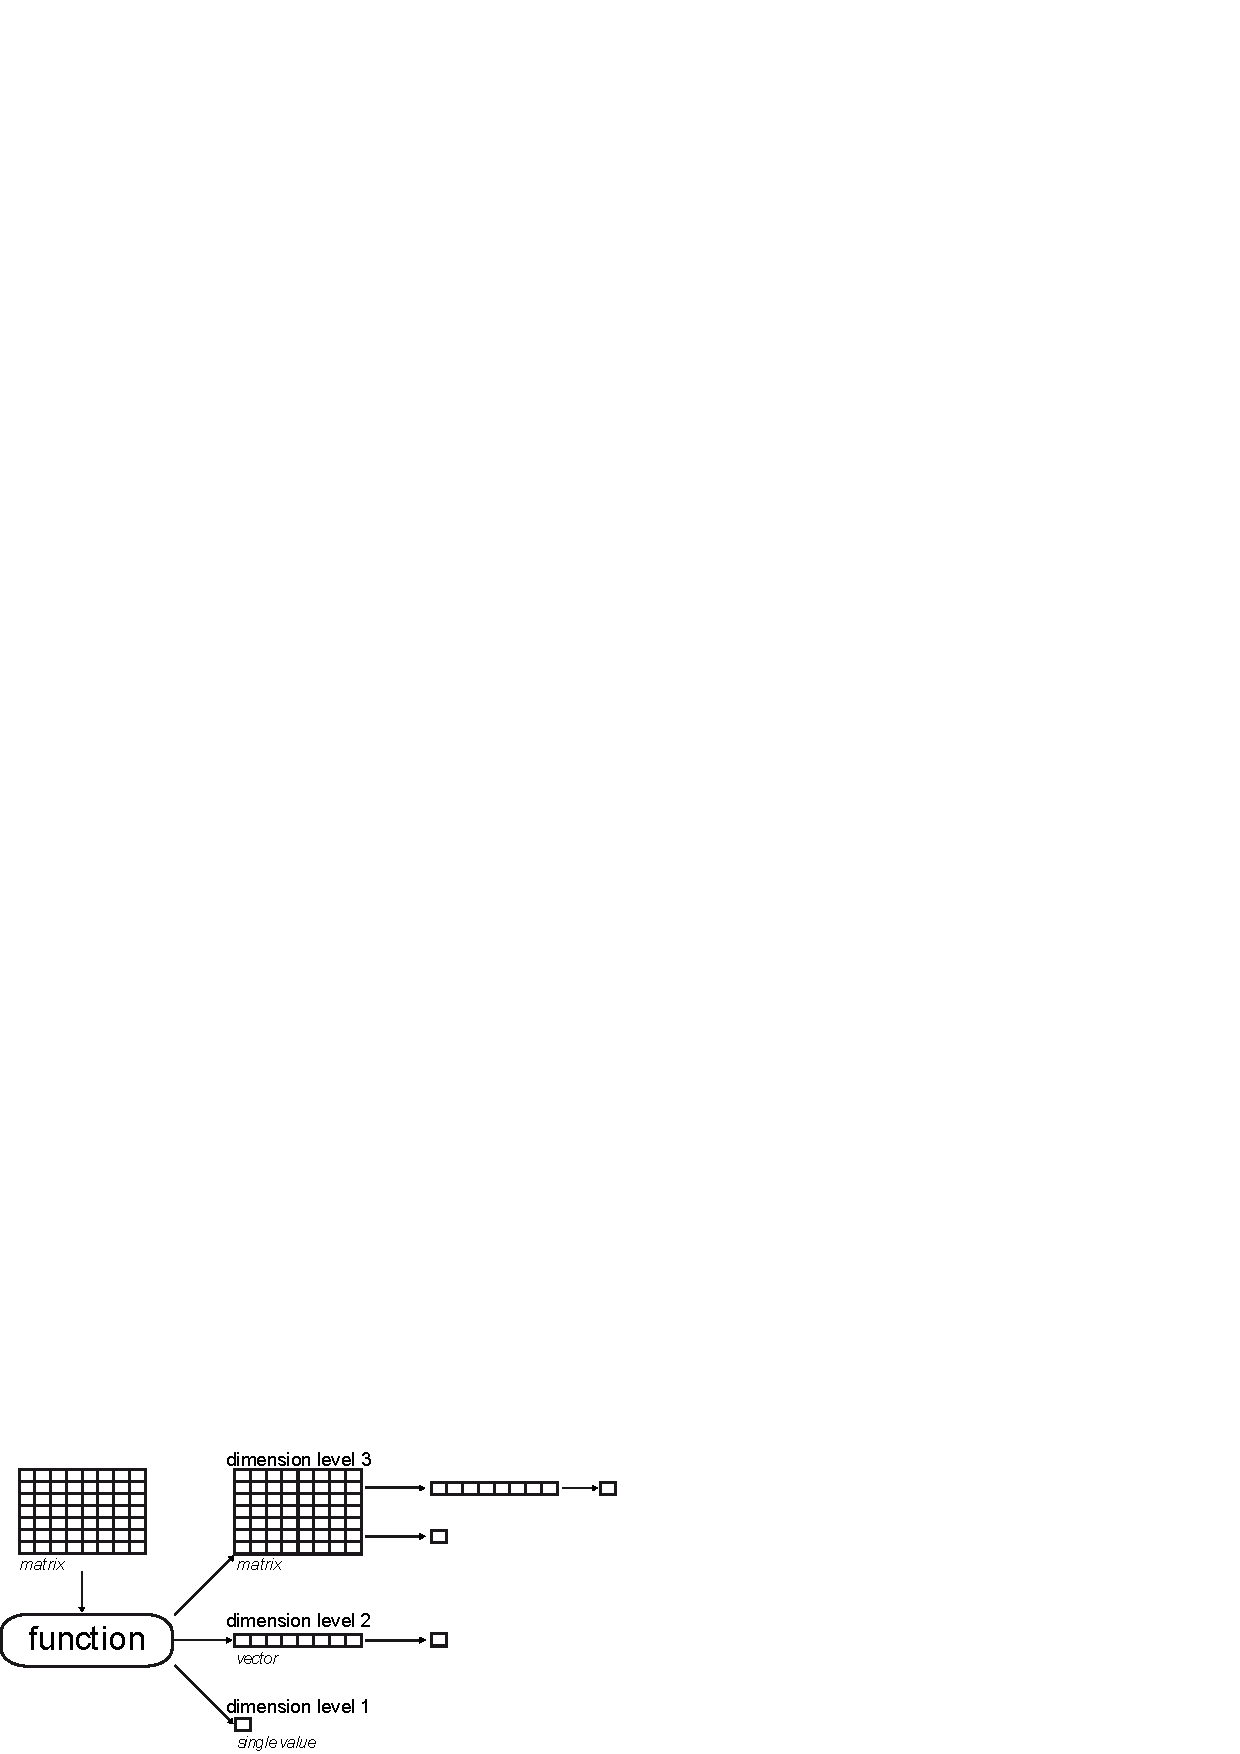
\includegraphics{dispRity_fun.png}
\caption{Illustration of the different dimension-levels of functions with an input \texttt{matrix}}
\end{figure}

\hypertarget{dimension-level-1-functions}{%
\subsubsection{Dimension-level 1 functions}\label{dimension-level-1-functions}}

A dimension-level 1 function will decompose a \texttt{matrix} or a \texttt{vector} into a single value:

\begin{Shaded}
\begin{Highlighting}[]
\CommentTok{\#\# Creating a dummy matrix}
\NormalTok{dummy\_matrix \textless{}{-}}\StringTok{ }\KeywordTok{matrix}\NormalTok{(}\KeywordTok{rnorm}\NormalTok{(}\DecValTok{12}\NormalTok{), }\DecValTok{4}\NormalTok{, }\DecValTok{3}\NormalTok{)}

\CommentTok{\#\# Example of dimension{-}level 1 functions}
\KeywordTok{mean}\NormalTok{(dummy\_matrix)}
\end{Highlighting}
\end{Shaded}

\begin{verbatim}
## [1] 0.1012674
\end{verbatim}

\begin{Shaded}
\begin{Highlighting}[]
\KeywordTok{median}\NormalTok{(dummy\_matrix)}
\end{Highlighting}
\end{Shaded}

\begin{verbatim}
## [1] 0.3345108
\end{verbatim}

Any summary metric such as mean or median are good examples of dimension-level 1 functions as they reduce the matrix to a single dimension (i.e.~one value).

\hypertarget{dimension-level-2-functions}{%
\subsubsection{Dimension-level 2 functions}\label{dimension-level-2-functions}}

A dimension-level 2 function will decompose a \texttt{matrix} into a \texttt{vector}.

\begin{Shaded}
\begin{Highlighting}[]
\CommentTok{\#\# Defining the function as the product of rows}
\NormalTok{prod.rows \textless{}{-}}\StringTok{ }\ControlFlowTok{function}\NormalTok{(matrix) }\KeywordTok{apply}\NormalTok{(matrix, }\DecValTok{1}\NormalTok{, prod)}

\CommentTok{\#\# A dimension{-}level 2 metric}
\KeywordTok{prod.rows}\NormalTok{(dummy\_matrix)}
\end{Highlighting}
\end{Shaded}

\begin{verbatim}
## [1]  0.72217818  2.48612354 -0.08986575  0.58266449
\end{verbatim}

Several dimension-level 2 functions are implemented in \texttt{dispRity} (see \texttt{?dispRity.metric}) such as the \texttt{variances} or \texttt{ranges} functions that calculate the variance or the range of each dimension of the ordinated matrix respectively.

\hypertarget{dimension-level-3-functions}{%
\subsubsection{Dimension-level 3 functions}\label{dimension-level-3-functions}}

Finally a dimension-level 3 function will transform the matrix into another matrix.
Note that the dimension of the output matrix doesn't need to match the the input matrix:

\begin{Shaded}
\begin{Highlighting}[]
\CommentTok{\#\# A dimension{-}level 3 metric}
\KeywordTok{var}\NormalTok{(dummy\_matrix)}
\end{Highlighting}
\end{Shaded}

\begin{verbatim}
##            [,1]       [,2]       [,3]
## [1,]  1.8570383  0.7417569 -0.5131686
## [2,]  0.7417569  1.3194330 -1.5344429
## [3,] -0.5131686 -1.5344429  2.8070556
\end{verbatim}

\begin{Shaded}
\begin{Highlighting}[]
\CommentTok{\#\# A dimension{-}level 3 metric with a forced matrix output}
\KeywordTok{as.matrix}\NormalTok{(}\KeywordTok{dist}\NormalTok{(dummy\_matrix))}
\end{Highlighting}
\end{Shaded}

\begin{verbatim}
##          1        2        3        4
## 1 0.000000 4.794738 3.382990 3.297110
## 2 4.794738 0.000000 2.400321 3.993864
## 3 3.382990 2.400321 0.000000 2.187412
## 4 3.297110 3.993864 2.187412 0.000000
\end{verbatim}

\hypertarget{betweengroupmetricsexplain}{%
\subsection{Between groups metrics}\label{betweengroupmetricsexplain}}

One specific category of metrics in the \texttt{dispRity} package is the between groups metrics.
As the name suggest, these metrics can be used to calculate the disparity between groups rather than within the groups.
These metrics follow the same classifications as the ``normal'' (within group) metrics with dimension-level 1, 2 and 3 between groups metrics.
However, at the difference of the ``normal'' metrics, their input arguments must be \texttt{matrix} and \texttt{matrix2} (and of course any other additional arguments).
For example, this metric measures the difference in mean between two matrices:

\begin{Shaded}
\begin{Highlighting}[]
\CommentTok{\#\# A simple example}
\NormalTok{mean.difference \textless{}{-}}\StringTok{ }\ControlFlowTok{function}\NormalTok{(matrix, matrix2) \{}
  \KeywordTok{mean}\NormalTok{(matrix) }\OperatorTok{{-}}\StringTok{ }\KeywordTok{mean}\NormalTok{(matrix2)}
\NormalTok{\}}
\end{Highlighting}
\end{Shaded}

You can find the list of implemented between groups metric \protect\hyperlink{betweengroupmetricslist}{here} or design them yourself for your specific needs (potentially using \protect\hyperlink{makemetric}{\texttt{make.metric}} for help).

The function works by simply using the two available matrices, with no restriction in terms of dimensions (although you'd probably want both matrices to have the same number of dimensions)

\begin{Shaded}
\begin{Highlighting}[]
\CommentTok{\#\# A second matrix}
\NormalTok{dummy\_matrix2 \textless{}{-}}\StringTok{ }\KeywordTok{matrix}\NormalTok{(}\KeywordTok{runif}\NormalTok{(}\DecValTok{12}\NormalTok{), }\DecValTok{4}\NormalTok{, }\DecValTok{3}\NormalTok{)}

\CommentTok{\#\# The difference between groups}
\KeywordTok{mean.difference}\NormalTok{(dummy\_matrix, dummy\_matrix2)}
\end{Highlighting}
\end{Shaded}

\begin{verbatim}
## [1] -0.3194556
\end{verbatim}

Beyond this super simple example, it might probably be interesting to use this metric on \texttt{dispRity} objects, especially the ones from \protect\hyperlink{custom-subsets}{\texttt{custom.subsets}} and \protect\hyperlink{chrono-subsets}{\texttt{chrono.subsets}}.
In fact, the \texttt{dispRity} function allows to apply the between groups metric directly to the \texttt{dispRity} objects using the \texttt{between.groups\ =\ TRUE} option.
For example:

\begin{Shaded}
\begin{Highlighting}[]
\CommentTok{\#\# Combining both matrices}
\NormalTok{big\_matrix \textless{}{-}}\StringTok{ }\KeywordTok{rbind}\NormalTok{(dummy\_matrix, dummy\_matrix2)}
\KeywordTok{rownames}\NormalTok{(big\_matrix) \textless{}{-}}\StringTok{ }\DecValTok{1}\OperatorTok{:}\DecValTok{8}

\CommentTok{\#\# Making a dispRity object with both groups}
\NormalTok{grouped\_matrix \textless{}{-}}\StringTok{ }\KeywordTok{custom.subsets}\NormalTok{(big\_matrix,}
                                 \DataTypeTok{group =} \KeywordTok{c}\NormalTok{(}\KeywordTok{list}\NormalTok{(}\DecValTok{1}\OperatorTok{:}\DecValTok{4}\NormalTok{), }\KeywordTok{list}\NormalTok{(}\DecValTok{1}\OperatorTok{:}\DecValTok{4}\NormalTok{)))}

\CommentTok{\#\# Calculating the mean difference between groups}
\NormalTok{(mean\_differences \textless{}{-}}\StringTok{ }\KeywordTok{dispRity}\NormalTok{(grouped\_matrix,}
                              \DataTypeTok{metric =}\NormalTok{ mean.difference,}
                              \DataTypeTok{between.groups =} \OtherTok{TRUE}\NormalTok{))}
\end{Highlighting}
\end{Shaded}

\begin{verbatim}
##  ---- dispRity object ---- 
## 2 customised subsets for 8 elements in one matrix with 3 dimensions:
##     1, 2.
## Disparity was calculated as: mean.difference between groups.
\end{verbatim}

\begin{Shaded}
\begin{Highlighting}[]
\CommentTok{\#\# Summarising the object}
\KeywordTok{summary}\NormalTok{(mean\_differences)}
\end{Highlighting}
\end{Shaded}

\begin{verbatim}
##   subsets n_1 n_2 obs
## 1     1:2   4   4   0
\end{verbatim}

\begin{Shaded}
\begin{Highlighting}[]
\CommentTok{\#\# Note how the summary table now indicates}
\CommentTok{\#\# the number of elements for each group}
\end{Highlighting}
\end{Shaded}

For \texttt{dispRity} objects generated by \texttt{custom.subsets}, the \texttt{dispRity} function will by default apply the metric on the groups in a pairwise fashion.
For example, if the object contains multiple groups, all groups will be compared to each other:

\begin{Shaded}
\begin{Highlighting}[]
\CommentTok{\#\# A dispRity object with multiple groups}
\NormalTok{grouped\_matrix \textless{}{-}}\StringTok{ }\KeywordTok{custom.subsets}\NormalTok{(big\_matrix,}
                                 \DataTypeTok{group =} \KeywordTok{c}\NormalTok{(}\StringTok{"A"}\NormalTok{ =}\StringTok{ }\KeywordTok{list}\NormalTok{(}\DecValTok{1}\OperatorTok{:}\DecValTok{4}\NormalTok{),}
                                           \StringTok{"B"}\NormalTok{ =}\StringTok{ }\KeywordTok{list}\NormalTok{(}\DecValTok{1}\OperatorTok{:}\DecValTok{4}\NormalTok{),}
                                           \StringTok{"C"}\NormalTok{ =}\StringTok{ }\KeywordTok{list}\NormalTok{(}\DecValTok{2}\OperatorTok{:}\DecValTok{6}\NormalTok{), }
                                           \StringTok{"D"}\NormalTok{ =}\StringTok{ }\KeywordTok{list}\NormalTok{(}\DecValTok{1}\OperatorTok{:}\DecValTok{8}\NormalTok{)))}

\CommentTok{\#\# Measuring disparity between all groups}
\KeywordTok{summary}\NormalTok{(}\KeywordTok{dispRity}\NormalTok{(grouped\_matrix, }\DataTypeTok{metric =}\NormalTok{ mean.difference,}
                 \DataTypeTok{between.groups =} \OtherTok{TRUE}\NormalTok{))}
\end{Highlighting}
\end{Shaded}

\begin{verbatim}
##   subsets n_1 n_2    obs
## 1     A:B   4   4  0.000
## 2     A:C   4   5 -0.172
## 3     A:D   4   8 -0.160
## 4     B:C   4   5 -0.172
## 5     B:D   4   8 -0.160
## 6     C:D   5   8  0.012
\end{verbatim}

For \texttt{dispRity} objects generated by \texttt{chrono.subsets} (not shown here), the \texttt{dispRity} function will by default apply the metric on the groups in a serial way (group 1 vs.~group 2, group 2 vs.~group 3, group 3 vs.~group 4, etc\ldots).
However, in both cases (for objects from \texttt{custom.subsets} or \texttt{chrono.subsets}) it is possible to manually specific the list of pairs of comparisons through their ID numbers:

\begin{Shaded}
\begin{Highlighting}[]
\CommentTok{\#\# Measuring disparity between specific groups}
\KeywordTok{summary}\NormalTok{(}\KeywordTok{dispRity}\NormalTok{(grouped\_matrix, }\DataTypeTok{metric =}\NormalTok{ mean.difference,}
                 \DataTypeTok{between.groups =} \KeywordTok{list}\NormalTok{(}\KeywordTok{c}\NormalTok{(}\DecValTok{1}\NormalTok{,}\DecValTok{3}\NormalTok{), }\KeywordTok{c}\NormalTok{(}\DecValTok{3}\NormalTok{,}\DecValTok{1}\NormalTok{), }\KeywordTok{c}\NormalTok{(}\DecValTok{4}\NormalTok{,}\DecValTok{1}\NormalTok{))))}
\end{Highlighting}
\end{Shaded}

\begin{verbatim}
##   subsets n_1 n_2    obs
## 1     A:C   4   5 -0.172
## 2     C:A   5   4  0.172
## 3     D:A   8   4  0.160
\end{verbatim}

Note that in any case, the order of the comparison can matter.
In our example, it is obvious that \texttt{mean(matrix)\ -\ mean(matrix2)} is not the same as \texttt{mean(matrix2)\ -\ mean(matrix)}.

\hypertarget{makemetric}{%
\subsection{\texorpdfstring{\texttt{make.metric}}{make.metric}}\label{makemetric}}

Of course, functions can be more complex and involve multiple operations such as the \texttt{centroids} function (see \texttt{?dispRity.metric}) that calculates the Euclidean distance between each element and the centroid of the ordinated space.
The \texttt{make.metric} function implemented in \texttt{dispRity} is designed to help test and find the dimension-level of the functions.
This function tests:

\begin{enumerate}
\def\labelenumi{\arabic{enumi}.}
\tightlist
\item
  If your function can deal with a \texttt{matrix} or a \texttt{vector} as an input;
\item
  Your function's dimension-level according to its output (dimension-level 1, 2 or 3, see above);
\item
  Whether the function can be implemented in the \texttt{dispRity} function (the function is fed into a \texttt{lapply} loop).
\end{enumerate}

For example, let's see if the functions described above are the right dimension-levels:

\begin{Shaded}
\begin{Highlighting}[]
\CommentTok{\#\# Which dimension{-}level is the mean function?}
\CommentTok{\#\# And can it be used in dispRity?}
\KeywordTok{make.metric}\NormalTok{(mean)}
\end{Highlighting}
\end{Shaded}

\begin{verbatim}
## mean outputs a single value.
## mean is detected as being a dimension-level 1 function.
\end{verbatim}

\begin{Shaded}
\begin{Highlighting}[]
\CommentTok{\#\# Which dimension{-}level is the prod.rows function?}
\CommentTok{\#\# And can it be used in dispRity?}
\KeywordTok{make.metric}\NormalTok{(prod.rows)}
\end{Highlighting}
\end{Shaded}

\begin{verbatim}
## prod.rows outputs a matrix object.
## prod.rows is detected as being a dimension-level 2 function.
\end{verbatim}

\begin{Shaded}
\begin{Highlighting}[]
\CommentTok{\#\# Which dimension{-}level is the var function?}
\CommentTok{\#\# And can it be used in dispRity?}
\KeywordTok{make.metric}\NormalTok{(var)}
\end{Highlighting}
\end{Shaded}

\begin{verbatim}
## var outputs a matrix object.
## var is detected as being a dimension-level 3 function.
## Additional dimension-level 2 and/or 1 function(s) will be needed.
\end{verbatim}

A non verbose version of the function is also available.
This can be done using the option \texttt{silent\ =\ TRUE} and will simply output the dimension-level of the metric.

\begin{Shaded}
\begin{Highlighting}[]
\CommentTok{\#\# Testing whether mean is dimension{-}level 1}
\ControlFlowTok{if}\NormalTok{(}\KeywordTok{make.metric}\NormalTok{(mean, }\DataTypeTok{silent =} \OtherTok{TRUE}\NormalTok{)}\OperatorTok{$}\NormalTok{type }\OperatorTok{!=}\StringTok{ "level1"}\NormalTok{) \{}
    \KeywordTok{message}\NormalTok{(}\StringTok{"The metric is not dimension{-}level 1."}\NormalTok{)}
\NormalTok{\}}
\CommentTok{\#\# Testing whether var is dimension{-}level 1}
\ControlFlowTok{if}\NormalTok{(}\KeywordTok{make.metric}\NormalTok{(var, }\DataTypeTok{silent =} \OtherTok{TRUE}\NormalTok{)}\OperatorTok{$}\NormalTok{type }\OperatorTok{!=}\StringTok{ "level1"}\NormalTok{) \{}
    \KeywordTok{message}\NormalTok{(}\StringTok{"The metric is not dimension{-}level 1."}\NormalTok{)}
\NormalTok{\}}
\end{Highlighting}
\end{Shaded}

\begin{verbatim}
## The metric is not dimension-level 1.
\end{verbatim}

\hypertarget{metrics-in-the-disprity-function}{%
\subsection{\texorpdfstring{Metrics in the \texttt{dispRity} function}{Metrics in the dispRity function}}\label{metrics-in-the-disprity-function}}

Using this metric structure, we can easily use any disparity metric in the \texttt{dispRity} function as follows:

\begin{Shaded}
\begin{Highlighting}[]
\CommentTok{\#\# Measuring disparity as the standard deviation}
\CommentTok{\#\# of all the values of the}
\CommentTok{\#\# ordinated matrix (dimension{-}level 1 function).}
\KeywordTok{summary}\NormalTok{(}\KeywordTok{dispRity}\NormalTok{(BeckLee\_mat50, }\DataTypeTok{metric =}\NormalTok{ sd))}
\end{Highlighting}
\end{Shaded}

\begin{verbatim}
##   subsets  n   obs
## 1       1 50 0.227
\end{verbatim}

\begin{Shaded}
\begin{Highlighting}[]
\CommentTok{\#\# Measuring disparity as the standard deviation}
\CommentTok{\#\# of the variance of each axis of}
\CommentTok{\#\# the ordinated matrix (dimension{-}level 1 and 2 functions).}
\KeywordTok{summary}\NormalTok{(}\KeywordTok{dispRity}\NormalTok{(BeckLee\_mat50, }\DataTypeTok{metric =} \KeywordTok{c}\NormalTok{(sd, variances)))}
\end{Highlighting}
\end{Shaded}

\begin{verbatim}
##   subsets  n   obs
## 1       1 50 0.032
\end{verbatim}

\begin{Shaded}
\begin{Highlighting}[]
\CommentTok{\#\# Measuring disparity as the standard deviation}
\CommentTok{\#\# of the variance of each axis of}
\CommentTok{\#\# the variance covariance matrix (dimension{-}level 1, 2 and 3 functions).}
\KeywordTok{summary}\NormalTok{(}\KeywordTok{dispRity}\NormalTok{(BeckLee\_mat50, }\DataTypeTok{metric =} \KeywordTok{c}\NormalTok{(sd, variances, var)), }\DataTypeTok{round =} \DecValTok{10}\NormalTok{)}
\end{Highlighting}
\end{Shaded}

\begin{verbatim}
##   subsets  n obs
## 1       1 50   0
\end{verbatim}

Note that the order of each function in the metric argument does not matter, the \texttt{dispRity} function will automatically detect the function dimension-levels (using \texttt{make.metric}) and apply them to the data in decreasing order (dimension-level 3 \textgreater{} 2 \textgreater{} 1).

\begin{Shaded}
\begin{Highlighting}[]
\CommentTok{\#\# Disparity as the standard deviation of the variance of each axis of the}
\CommentTok{\#\# variance covariance matrix:}
\NormalTok{disparity1 \textless{}{-}}\StringTok{ }\KeywordTok{summary}\NormalTok{(}\KeywordTok{dispRity}\NormalTok{(BeckLee\_mat50,}
                               \DataTypeTok{metric =} \KeywordTok{c}\NormalTok{(sd, variances, var)),}
                      \DataTypeTok{round =} \DecValTok{10}\NormalTok{)}

\CommentTok{\#\# Same as above but using a different function order for the metric argument}
\NormalTok{disparity2 \textless{}{-}}\StringTok{ }\KeywordTok{summary}\NormalTok{(}\KeywordTok{dispRity}\NormalTok{(BeckLee\_mat50,}
                               \DataTypeTok{metric =} \KeywordTok{c}\NormalTok{(variances, sd, var)),}
                      \DataTypeTok{round =} \DecValTok{10}\NormalTok{)}

\CommentTok{\#\# Both ways output the same disparity values:}
\NormalTok{disparity1 }\OperatorTok{==}\StringTok{ }\NormalTok{disparity2}
\end{Highlighting}
\end{Shaded}

\begin{verbatim}
##      subsets    n  obs
## [1,]    TRUE TRUE TRUE
\end{verbatim}

In these examples, we considered disparity to be a single value.
For example, in the previous example, we defined disparity as the standard deviation of the variances of each column of the variance/covariance matrix (\texttt{metric\ =\ c(variances,\ sd,\ var)}).
It is, however, possible to calculate \protect\hyperlink{disparity-as-a-distribution}{disparity as a distribution}.

\hypertarget{metrics-implemented-in-disprity}{%
\subsection{\texorpdfstring{Metrics implemented in \texttt{dispRity}}{Metrics implemented in dispRity}}\label{metrics-implemented-in-disprity}}

Several disparity metrics are implemented in the \texttt{dispRity} package.
The detailed list can be found in \texttt{?dispRity.metric} along with some description of each metric.

\begin{longtable}[]{@{}llll@{}}
\toprule
\begin{minipage}[b]{0.07\columnwidth}\raggedright
Level\strut
\end{minipage} & \begin{minipage}[b]{0.07\columnwidth}\raggedright
Name\strut
\end{minipage} & \begin{minipage}[b]{0.64\columnwidth}\raggedright
Description\strut
\end{minipage} & \begin{minipage}[b]{0.10\columnwidth}\raggedright
Source\strut
\end{minipage}\tabularnewline
\midrule
\endhead
\begin{minipage}[t]{0.07\columnwidth}\raggedright
2\strut
\end{minipage} & \begin{minipage}[t]{0.07\columnwidth}\raggedright
\texttt{ancestral.dist}\strut
\end{minipage} & \begin{minipage}[t]{0.64\columnwidth}\raggedright
The distance between an element and its ancestor\strut
\end{minipage} & \begin{minipage}[t]{0.10\columnwidth}\raggedright
\texttt{dispRity}\strut
\end{minipage}\tabularnewline
\begin{minipage}[t]{0.07\columnwidth}\raggedright
2\strut
\end{minipage} & \begin{minipage}[t]{0.07\columnwidth}\raggedright
\texttt{angles}\strut
\end{minipage} & \begin{minipage}[t]{0.64\columnwidth}\raggedright
The angle of main variation of each dimensions\strut
\end{minipage} & \begin{minipage}[t]{0.10\columnwidth}\raggedright
\texttt{dispRity}\strut
\end{minipage}\tabularnewline
\begin{minipage}[t]{0.07\columnwidth}\raggedright
2\strut
\end{minipage} & \begin{minipage}[t]{0.07\columnwidth}\raggedright
\texttt{centroids}1\strut
\end{minipage} & \begin{minipage}[t]{0.64\columnwidth}\raggedright
The distance between each element and the centroid of the ordinated space\strut
\end{minipage} & \begin{minipage}[t]{0.10\columnwidth}\raggedright
\texttt{dispRity}\strut
\end{minipage}\tabularnewline
\begin{minipage}[t]{0.07\columnwidth}\raggedright
1\strut
\end{minipage} & \begin{minipage}[t]{0.07\columnwidth}\raggedright
\texttt{convhull.surface}\strut
\end{minipage} & \begin{minipage}[t]{0.64\columnwidth}\raggedright
The surface of the convex hull formed by all the elements\strut
\end{minipage} & \begin{minipage}[t]{0.10\columnwidth}\raggedright
\href{https://cran.r-project.org/web/packages/geometry/index.html}{\texttt{geometry}}\texttt{::convhulln\$area}\strut
\end{minipage}\tabularnewline
\begin{minipage}[t]{0.07\columnwidth}\raggedright
1\strut
\end{minipage} & \begin{minipage}[t]{0.07\columnwidth}\raggedright
\texttt{convhull.volume}\strut
\end{minipage} & \begin{minipage}[t]{0.64\columnwidth}\raggedright
The volume of the convex hull formed by all the elements\strut
\end{minipage} & \begin{minipage}[t]{0.10\columnwidth}\raggedright
\href{https://cran.r-project.org/web/packages/geometry/index.html}{\texttt{geometry}}\texttt{::convhulln\$vol}\strut
\end{minipage}\tabularnewline
\begin{minipage}[t]{0.07\columnwidth}\raggedright
2\strut
\end{minipage} & \begin{minipage}[t]{0.07\columnwidth}\raggedright
\texttt{deviations}\strut
\end{minipage} & \begin{minipage}[t]{0.64\columnwidth}\raggedright
The minimal distance between each element and a hyperplane\strut
\end{minipage} & \begin{minipage}[t]{0.10\columnwidth}\raggedright
\texttt{dispRity}\strut
\end{minipage}\tabularnewline
\begin{minipage}[t]{0.07\columnwidth}\raggedright
1\strut
\end{minipage} & \begin{minipage}[t]{0.07\columnwidth}\raggedright
\texttt{diagonal}\strut
\end{minipage} & \begin{minipage}[t]{0.64\columnwidth}\raggedright
The longest distance in the ordinated space (like the diagonal in two dimensions)\strut
\end{minipage} & \begin{minipage}[t]{0.10\columnwidth}\raggedright
\texttt{dispRity}\strut
\end{minipage}\tabularnewline
\begin{minipage}[t]{0.07\columnwidth}\raggedright
1\strut
\end{minipage} & \begin{minipage}[t]{0.07\columnwidth}\raggedright
\texttt{disalignment}\strut
\end{minipage} & \begin{minipage}[t]{0.64\columnwidth}\raggedright
The rejection of the centroid of a matrix from the major axis of another (typically an \texttt{"as.covar"} metric)\strut
\end{minipage} & \begin{minipage}[t]{0.10\columnwidth}\raggedright
\texttt{dispRity}\strut
\end{minipage}\tabularnewline
\begin{minipage}[t]{0.07\columnwidth}\raggedright
2\strut
\end{minipage} & \begin{minipage}[t]{0.07\columnwidth}\raggedright
\texttt{displacements}\strut
\end{minipage} & \begin{minipage}[t]{0.64\columnwidth}\raggedright
The ratio between the distance from a reference and the distance from the centroid\strut
\end{minipage} & \begin{minipage}[t]{0.10\columnwidth}\raggedright
\texttt{dispRity}\strut
\end{minipage}\tabularnewline
\begin{minipage}[t]{0.07\columnwidth}\raggedright
1\strut
\end{minipage} & \begin{minipage}[t]{0.07\columnwidth}\raggedright
\texttt{edge.length.tree}\strut
\end{minipage} & \begin{minipage}[t]{0.64\columnwidth}\raggedright
The edge lengths of the elements on a tree\strut
\end{minipage} & \begin{minipage}[t]{0.10\columnwidth}\raggedright
\texttt{ape}\strut
\end{minipage}\tabularnewline
\begin{minipage}[t]{0.07\columnwidth}\raggedright
1\strut
\end{minipage} & \begin{minipage}[t]{0.07\columnwidth}\raggedright
\texttt{ellipse.volume}1\strut
\end{minipage} & \begin{minipage}[t]{0.64\columnwidth}\raggedright
The volume of the ellipsoid of the space\strut
\end{minipage} & \begin{minipage}[t]{0.10\columnwidth}\raggedright
Donohue \emph{et al.} (2013)\strut
\end{minipage}\tabularnewline
\begin{minipage}[t]{0.07\columnwidth}\raggedright
1\strut
\end{minipage} & \begin{minipage}[t]{0.07\columnwidth}\raggedright
\texttt{func.div}\strut
\end{minipage} & \begin{minipage}[t]{0.64\columnwidth}\raggedright
The functional divergence (the ratio of deviation from the centroid)\strut
\end{minipage} & \begin{minipage}[t]{0.10\columnwidth}\raggedright
\texttt{dispRity} (similar to \href{https://cran.r-project.org/web/packages/FD/index.html}{\texttt{FD}}\texttt{::dbFD\$FDiv} but without abundance)\strut
\end{minipage}\tabularnewline
\begin{minipage}[t]{0.07\columnwidth}\raggedright
1\strut
\end{minipage} & \begin{minipage}[t]{0.07\columnwidth}\raggedright
\texttt{func.eve}\strut
\end{minipage} & \begin{minipage}[t]{0.64\columnwidth}\raggedright
The functional evenness (the minimal spanning tree distances evenness)\strut
\end{minipage} & \begin{minipage}[t]{0.10\columnwidth}\raggedright
\texttt{dispRity} (similar to \href{https://cran.r-project.org/web/packages/FD/index.html}{\texttt{FD}}\texttt{::dbFD\$FEve} but without abundance)\strut
\end{minipage}\tabularnewline
\begin{minipage}[t]{0.07\columnwidth}\raggedright
1\strut
\end{minipage} & \begin{minipage}[t]{0.07\columnwidth}\raggedright
\texttt{group.dist}\strut
\end{minipage} & \begin{minipage}[t]{0.64\columnwidth}\raggedright
The distance between two groups\strut
\end{minipage} & \begin{minipage}[t]{0.10\columnwidth}\raggedright
\texttt{dispRity}\strut
\end{minipage}\tabularnewline
\begin{minipage}[t]{0.07\columnwidth}\raggedright
1\strut
\end{minipage} & \begin{minipage}[t]{0.07\columnwidth}\raggedright
\texttt{mode.val}\strut
\end{minipage} & \begin{minipage}[t]{0.64\columnwidth}\raggedright
The modal value\strut
\end{minipage} & \begin{minipage}[t]{0.10\columnwidth}\raggedright
\texttt{dispRity}\strut
\end{minipage}\tabularnewline
\begin{minipage}[t]{0.07\columnwidth}\raggedright
1\strut
\end{minipage} & \begin{minipage}[t]{0.07\columnwidth}\raggedright
\texttt{n.ball.volume}\strut
\end{minipage} & \begin{minipage}[t]{0.64\columnwidth}\raggedright
The hyper-spherical (\emph{n}-ball) volume\strut
\end{minipage} & \begin{minipage}[t]{0.10\columnwidth}\raggedright
\texttt{dispRity}\strut
\end{minipage}\tabularnewline
\begin{minipage}[t]{0.07\columnwidth}\raggedright
2\strut
\end{minipage} & \begin{minipage}[t]{0.07\columnwidth}\raggedright
\texttt{neighbours}\strut
\end{minipage} & \begin{minipage}[t]{0.64\columnwidth}\raggedright
The distance to specific neighbours (e.g.~the nearest neighbours - by default)\strut
\end{minipage} & \begin{minipage}[t]{0.10\columnwidth}\raggedright
\texttt{dispRity}\strut
\end{minipage}\tabularnewline
\begin{minipage}[t]{0.07\columnwidth}\raggedright
2\strut
\end{minipage} & \begin{minipage}[t]{0.07\columnwidth}\raggedright
\texttt{pairwise.dist}\strut
\end{minipage} & \begin{minipage}[t]{0.64\columnwidth}\raggedright
The pairwise distances between elements\strut
\end{minipage} & \begin{minipage}[t]{0.10\columnwidth}\raggedright
\href{https://cran.r-project.org/web/packages/vegan/index.html}{\texttt{vegan}}\texttt{::vegist}\strut
\end{minipage}\tabularnewline
\begin{minipage}[t]{0.07\columnwidth}\raggedright
2\strut
\end{minipage} & \begin{minipage}[t]{0.07\columnwidth}\raggedright
\texttt{point.dist}\strut
\end{minipage} & \begin{minipage}[t]{0.64\columnwidth}\raggedright
The distance between one group and the point of another group\strut
\end{minipage} & \begin{minipage}[t]{0.10\columnwidth}\raggedright
\texttt{dispRity}\strut
\end{minipage}\tabularnewline
\begin{minipage}[t]{0.07\columnwidth}\raggedright
2\strut
\end{minipage} & \begin{minipage}[t]{0.07\columnwidth}\raggedright
\texttt{projections}\strut
\end{minipage} & \begin{minipage}[t]{0.64\columnwidth}\raggedright
The distance \emph{on} (projection) or \emph{from} (rejection) an arbitrary vector\strut
\end{minipage} & \begin{minipage}[t]{0.10\columnwidth}\raggedright
\texttt{dispRity}\strut
\end{minipage}\tabularnewline
\begin{minipage}[t]{0.07\columnwidth}\raggedright
1\strut
\end{minipage} & \begin{minipage}[t]{0.07\columnwidth}\raggedright
\texttt{projections.between}\strut
\end{minipage} & \begin{minipage}[t]{0.64\columnwidth}\raggedright
\texttt{projections} metric applied between groups\strut
\end{minipage} & \begin{minipage}[t]{0.10\columnwidth}\raggedright
\texttt{dispRity}\strut
\end{minipage}\tabularnewline
\begin{minipage}[t]{0.07\columnwidth}\raggedright
2\strut
\end{minipage} & \begin{minipage}[t]{0.07\columnwidth}\raggedright
\texttt{projections.tree}\strut
\end{minipage} & \begin{minipage}[t]{0.64\columnwidth}\raggedright
The \texttt{projections} metric but where the vector can be based on a tree\strut
\end{minipage} & \begin{minipage}[t]{0.10\columnwidth}\raggedright
\texttt{dispRity}\strut
\end{minipage}\tabularnewline
\begin{minipage}[t]{0.07\columnwidth}\raggedright
2\strut
\end{minipage} & \begin{minipage}[t]{0.07\columnwidth}\raggedright
\texttt{quantiles}\strut
\end{minipage} & \begin{minipage}[t]{0.64\columnwidth}\raggedright
The \emph{n}th quantile range per axis\strut
\end{minipage} & \begin{minipage}[t]{0.10\columnwidth}\raggedright
\texttt{dispRity}\strut
\end{minipage}\tabularnewline
\begin{minipage}[t]{0.07\columnwidth}\raggedright
2\strut
\end{minipage} & \begin{minipage}[t]{0.07\columnwidth}\raggedright
\texttt{radius}\strut
\end{minipage} & \begin{minipage}[t]{0.64\columnwidth}\raggedright
The radius of each dimensions\strut
\end{minipage} & \begin{minipage}[t]{0.10\columnwidth}\raggedright
\texttt{dispRity}\strut
\end{minipage}\tabularnewline
\begin{minipage}[t]{0.07\columnwidth}\raggedright
2\strut
\end{minipage} & \begin{minipage}[t]{0.07\columnwidth}\raggedright
\texttt{ranges}\strut
\end{minipage} & \begin{minipage}[t]{0.64\columnwidth}\raggedright
The range of each dimension\strut
\end{minipage} & \begin{minipage}[t]{0.10\columnwidth}\raggedright
\texttt{dispRity}\strut
\end{minipage}\tabularnewline
\begin{minipage}[t]{0.07\columnwidth}\raggedright
2\strut
\end{minipage} & \begin{minipage}[t]{0.07\columnwidth}\raggedright
\texttt{span.tree.length}\strut
\end{minipage} & \begin{minipage}[t]{0.64\columnwidth}\raggedright
The minimal spanning tree length\strut
\end{minipage} & \begin{minipage}[t]{0.10\columnwidth}\raggedright
\href{https://cran.r-project.org/web/packages/vegan/index.html}{\texttt{vegan}}\texttt{::spantree}\strut
\end{minipage}\tabularnewline
\begin{minipage}[t]{0.07\columnwidth}\raggedright
2\strut
\end{minipage} & \begin{minipage}[t]{0.07\columnwidth}\raggedright
\texttt{variances}\strut
\end{minipage} & \begin{minipage}[t]{0.64\columnwidth}\raggedright
The variance of each dimension\strut
\end{minipage} & \begin{minipage}[t]{0.10\columnwidth}\raggedright
\texttt{dispRity}\strut
\end{minipage}\tabularnewline
\bottomrule
\end{longtable}

1: Note that by default, the centroid is the centroid of the elements.
It can, however, be fixed to a different value by using the \texttt{centroid} argument \texttt{centroids(space,\ centroid\ =\ rep(0,\ ncol(space)))}, for example the origin of the ordinated space.

2: This function uses an estimation of the eigenvalue that only works for MDS or PCoA ordinations (\emph{not} PCA).

You can find more informations on the vast variety of metrics that you can use in your analysis in this \href{https://www.biorxiv.org/content/10.1101/801571v1}{preprint}.

\hypertarget{equations-and-implementations}{%
\subsection{Equations and implementations}\label{equations-and-implementations}}

Some of the functions described below are implemented in the \texttt{dispRity} package and do not require any other packages to calculate (\href{https://github.com/TGuillerme/dispRity/blob/master/R/dispRity.metric.R}{see implementation here}).

\begin{equation}
    ancestral.dist = \sqrt{\sum_{i=1}^{n}{({d}_{n}-Ancestor_{n})^2}}
\end{equation}

\begin{equation}
    centroids = \sqrt{\sum_{i=1}^{n}{({d}_{n}-Centroid_{d})^2}}
\end{equation}

\begin{equation}
    diagonal = \sqrt{\sum_{i=1}^{d}|max(d_i) - min(k_i)|}
\end{equation}

\begin{equation}
    deviations = \frac{|Ax + By + ... + Nm + Intercept|}{\sqrt{A^2 + B^2 + ... + N^2}}
\end{equation}

\begin{equation}
    displacements = \frac{\sqrt{\sum_{i=1}^{n}{({d}_{n}-Reference_{d})^2}}}{\sqrt{\sum_{i=1}^{n}{({d}_{n}-Centroid_{k})^2}}}
\end{equation}

\begin{equation}
    ellipse.volume = \frac{\pi^{d/2}}{\Gamma(\frac{d}{2}+1)}\displaystyle\prod_{i=1}^{d} (\lambda_{i}^{0.5})
\end{equation}

\begin{equation}
    n.ball.volume = \frac{\pi^{d/2}}{\Gamma(\frac{d}{2}+1)}\displaystyle\prod_{i=1}^{d} R
\end{equation}

\begin{equation}
    projection_{on} = \| \overrightarrow{i} \cdot \overrightarrow{b} \|
\end{equation}
\begin{equation}
    projection_{from} = \| \overrightarrow{i} - \overrightarrow{i} \cdot \overrightarrow{b} \|
\end{equation}

\begin{equation}
    radius = |\frac{\sum_{i=1}^{n}d_i}{n} - f(\mathbf{v}d)|
\end{equation}

\begin{equation}
    ranges = |max(d_i) - min(d_i)|
\end{equation}

\begin{equation}
    variances = \sigma^{2}{d_i}
\end{equation}

\begin{equation}
    span.tree.length = \mathrm{branch\ length}
\end{equation}

Where \emph{d} is the number of dimensions,
\emph{n} the number of elements,
\(\Gamma\) is the Gamma distribution,
\(\lambda_i\) is the eigenvalue of each dimensions,
\(\sigma^{2}\) is their variance and
\(Centroid_{k}\) is their mean,
\(Ancestor_{n}\) is the coordinates of the ancestor of element \(n\),
\(f(\mathbf{v}k)\) is function to select one value from the vector \(\mathbf{v}\) of the dimension \(k\) (e.g.~it's maximum, minimum, mean, etc.),
\emph{R} is the radius of the sphere or the product of the radii of each dimensions (\(\displaystyle\prod_{i=1}^{k}R_{i}\) - for a hyper-ellipsoid),
\(Reference_{k}\) is an arbitrary point's coordinates (usually 0),
\(\overrightarrow{b}\) is the vector defined by (\texttt{(point1,\ point2)}),
and \(\overrightarrow{i}\) is the vector defined by (\texttt{(point1,\ i)} where \texttt{i} is any row of the matrix).

\hypertarget{using-the-different-disparity-metrics}{%
\subsection{Using the different disparity metrics}\label{using-the-different-disparity-metrics}}

Here is a brief demonstration of the main metrics implemented in \texttt{dispRity}.
First, we will create a dummy/simulated ordinated space using the \texttt{space.maker} utility function (more about that \protect\hyperlink{space.maker}{here}:

\begin{Shaded}
\begin{Highlighting}[]
\CommentTok{\#\# Creating a 10*5 normal space}
\KeywordTok{set.seed}\NormalTok{(}\DecValTok{1}\NormalTok{)}
\NormalTok{dummy\_space \textless{}{-}}\StringTok{ }\KeywordTok{space.maker}\NormalTok{(}\DecValTok{10}\NormalTok{, }\DecValTok{5}\NormalTok{, rnorm)}
\KeywordTok{rownames}\NormalTok{(dummy\_space) \textless{}{-}}\StringTok{ }\DecValTok{1}\OperatorTok{:}\DecValTok{10}
\end{Highlighting}
\end{Shaded}

We will use this simulated space to demonstrate the different metrics.

\hypertarget{volumes-and-surface-metrics}{%
\subsubsection{Volumes and surface metrics}\label{volumes-and-surface-metrics}}

The functions \texttt{ellipse.volume}, \texttt{convhull.surface}, \texttt{convhull.volume} and \texttt{n.ball.volume} all measure the surface or the volume of the ordinated space occupied:

Because there is only one subset (i.e.~one matrix) in the dispRity object, the operations below are the equivalent of \texttt{metric(dummy\_space)} (with rounding).

\begin{Shaded}
\begin{Highlighting}[]
\CommentTok{\#\# Calculating the ellipsoid volume}
\KeywordTok{summary}\NormalTok{(}\KeywordTok{dispRity}\NormalTok{(dummy\_space, }\DataTypeTok{metric =}\NormalTok{ ellipse.volume))}
\end{Highlighting}
\end{Shaded}

\begin{verbatim}
##   subsets  n   obs
## 1       1 10 1.061
\end{verbatim}

\begin{quote}
WARNING: in such dummy space, this gives the estimation of the ellipsoid volume, not the real ellipsoid volume! See the cautionary note in \texttt{?ellipse.volume}.
\end{quote}

\begin{Shaded}
\begin{Highlighting}[]
\CommentTok{\#\# Calculating the convex hull surface}
\KeywordTok{summary}\NormalTok{(}\KeywordTok{dispRity}\NormalTok{(dummy\_space, }\DataTypeTok{metric =}\NormalTok{ convhull.surface))}
\end{Highlighting}
\end{Shaded}

\begin{verbatim}
##   subsets  n   obs
## 1       1 10 11.91
\end{verbatim}

\begin{Shaded}
\begin{Highlighting}[]
\CommentTok{\#\# Calculating the convex hull volume}
\KeywordTok{summary}\NormalTok{(}\KeywordTok{dispRity}\NormalTok{(dummy\_space, }\DataTypeTok{metric =}\NormalTok{ convhull.volume))}
\end{Highlighting}
\end{Shaded}

\begin{verbatim}
##   subsets  n   obs
## 1       1 10 1.031
\end{verbatim}

\begin{Shaded}
\begin{Highlighting}[]
\CommentTok{\#\# Calculating the convex hull volume}
\KeywordTok{summary}\NormalTok{(}\KeywordTok{dispRity}\NormalTok{(dummy\_space, }\DataTypeTok{metric =}\NormalTok{ n.ball.volume))}
\end{Highlighting}
\end{Shaded}

\begin{verbatim}
##   subsets  n  obs
## 1       1 10 4.43
\end{verbatim}

The convex hull based functions are a call to the \texttt{geometry::convhulln} function with the \texttt{"FA"} option (computes total area and volume).
Also note that they are really sensitive to the size of the dataset.

\begin{quote}
Cautionary note: measuring volumes in a high number of dimensions can be strongly affected by the \href{https://en.wikipedia.org/wiki/Curse_of_dimensionality}{curse of dimensionality} that often results in near 0 disparity values. I strongly recommend reading \href{https://beta.observablehq.com/@tophtucker/theres-plenty-of-room-in-the-corners}{this really intuitive explanation} from \href{https://github.com/tophtucker}{Toph Tucker}.
\end{quote}

\hypertarget{ranges-variances-quantiles-radius-pairwise-distance-neighbours-modal-value-and-diagonal}{%
\subsubsection{Ranges, variances, quantiles, radius, pairwise distance, neighbours, modal value and diagonal}\label{ranges-variances-quantiles-radius-pairwise-distance-neighbours-modal-value-and-diagonal}}

The functions \texttt{ranges}, \texttt{variances} \texttt{radius}, \texttt{pairwise.dist}, \texttt{mode.val} and \texttt{diagonal} all measure properties of the ordinated space based on its dimensional properties (they are also less affected by the ``curse of dimensionality''):

\texttt{ranges}, \texttt{variances} \texttt{quantiles} and \texttt{radius} work on the same principle and measure the range/variance/radius of each dimension:

\begin{Shaded}
\begin{Highlighting}[]
\CommentTok{\#\# Calculating the ranges of each dimension in the ordinated space}
\KeywordTok{ranges}\NormalTok{(dummy\_space)}
\end{Highlighting}
\end{Shaded}

\begin{verbatim}
## [1] 2.430909 3.726481 2.908329 2.735739 1.588603
\end{verbatim}

\begin{Shaded}
\begin{Highlighting}[]
\CommentTok{\#\# Calculating disparity as the distribution of these ranges}
\KeywordTok{summary}\NormalTok{(}\KeywordTok{dispRity}\NormalTok{(dummy\_space, }\DataTypeTok{metric =}\NormalTok{ ranges))}
\end{Highlighting}
\end{Shaded}

\begin{verbatim}
##   subsets  n obs.median  2.5%   25%   75% 97.5%
## 1       1 10      2.736 1.673 2.431 2.908 3.645
\end{verbatim}

\begin{Shaded}
\begin{Highlighting}[]
\CommentTok{\#\# Calculating disparity as the sum and the product of these ranges}
\KeywordTok{summary}\NormalTok{(}\KeywordTok{dispRity}\NormalTok{(dummy\_space, }\DataTypeTok{metric =} \KeywordTok{c}\NormalTok{(sum, ranges)))}
\end{Highlighting}
\end{Shaded}

\begin{verbatim}
##   subsets  n   obs
## 1       1 10 13.39
\end{verbatim}

\begin{Shaded}
\begin{Highlighting}[]
\KeywordTok{summary}\NormalTok{(}\KeywordTok{dispRity}\NormalTok{(dummy\_space, }\DataTypeTok{metric =} \KeywordTok{c}\NormalTok{(prod, ranges)))}
\end{Highlighting}
\end{Shaded}

\begin{verbatim}
##   subsets  n   obs
## 1       1 10 114.5
\end{verbatim}

\begin{Shaded}
\begin{Highlighting}[]
\CommentTok{\#\# Calculating the variances of each dimension in the}
\CommentTok{\#\# ordinated space}
\KeywordTok{variances}\NormalTok{(dummy\_space)}
\end{Highlighting}
\end{Shaded}

\begin{verbatim}
## [1] 0.6093144 1.1438620 0.9131859 0.6537768 0.3549372
\end{verbatim}

\begin{Shaded}
\begin{Highlighting}[]
\CommentTok{\#\# Calculating disparity as the distribution of these variances}
\KeywordTok{summary}\NormalTok{(}\KeywordTok{dispRity}\NormalTok{(dummy\_space, }\DataTypeTok{metric =}\NormalTok{ variances))}
\end{Highlighting}
\end{Shaded}

\begin{verbatim}
##   subsets  n obs.median 2.5%   25%   75% 97.5%
## 1       1 10      0.654 0.38 0.609 0.913 1.121
\end{verbatim}

\begin{Shaded}
\begin{Highlighting}[]
\CommentTok{\#\# Calculating disparity as the sum and}
\CommentTok{\#\# the product of these variances}
\KeywordTok{summary}\NormalTok{(}\KeywordTok{dispRity}\NormalTok{(dummy\_space, }\DataTypeTok{metric =} \KeywordTok{c}\NormalTok{(sum, variances)))}
\end{Highlighting}
\end{Shaded}

\begin{verbatim}
##   subsets  n   obs
## 1       1 10 3.675
\end{verbatim}

\begin{Shaded}
\begin{Highlighting}[]
\KeywordTok{summary}\NormalTok{(}\KeywordTok{dispRity}\NormalTok{(dummy\_space, }\DataTypeTok{metric =} \KeywordTok{c}\NormalTok{(prod, variances)))}
\end{Highlighting}
\end{Shaded}

\begin{verbatim}
##   subsets  n   obs
## 1       1 10 0.148
\end{verbatim}

\begin{Shaded}
\begin{Highlighting}[]
\CommentTok{\#\# Calculating the quantiles of each dimension}
\CommentTok{\#\# in the ordinated space}
\KeywordTok{quantiles}\NormalTok{(dummy\_space)}
\end{Highlighting}
\end{Shaded}

\begin{verbatim}
## [1] 2.234683 3.280911 2.760855 2.461077 1.559057
\end{verbatim}

\begin{Shaded}
\begin{Highlighting}[]
\CommentTok{\#\# Calculating disparity as the distribution of these variances}
\KeywordTok{summary}\NormalTok{(}\KeywordTok{dispRity}\NormalTok{(dummy\_space, }\DataTypeTok{metric =}\NormalTok{ quantiles))}
\end{Highlighting}
\end{Shaded}

\begin{verbatim}
##   subsets  n obs.median  2.5%   25%   75% 97.5%
## 1       1 10      2.461 1.627 2.235 2.761 3.229
\end{verbatim}

\begin{Shaded}
\begin{Highlighting}[]
\CommentTok{\#\# By default, the quantile calculated is the 95\%}
\CommentTok{\#\# (i.e. 95\% of the data on each axis)}
\CommentTok{\#\# this can be changed using the option quantile:}
\KeywordTok{summary}\NormalTok{(}\KeywordTok{dispRity}\NormalTok{(dummy\_space, }\DataTypeTok{metric =}\NormalTok{ quantiles, }\DataTypeTok{quantile =} \DecValTok{50}\NormalTok{))}
\end{Highlighting}
\end{Shaded}

\begin{verbatim}
##   subsets  n obs.median  2.5%   25%   75% 97.5%
## 1       1 10      0.967 0.899 0.951 0.991 1.089
\end{verbatim}

\begin{Shaded}
\begin{Highlighting}[]
\CommentTok{\#\# Calculating the radius of each dimension in the ordinated space}
\KeywordTok{radius}\NormalTok{(dummy\_space)}
\end{Highlighting}
\end{Shaded}

\begin{verbatim}
## [1] 1.4630780 2.4635449 1.8556785 1.4977898 0.8416318
\end{verbatim}

\begin{Shaded}
\begin{Highlighting}[]
\CommentTok{\#\# By default the radius is the maximum distance from the centre of}
\CommentTok{\#\# the dimension. It can however be changed to any function:}
\KeywordTok{radius}\NormalTok{(dummy\_space, }\DataTypeTok{type =}\NormalTok{ min)}
\end{Highlighting}
\end{Shaded}

\begin{verbatim}
## [1] 0.05144054 0.14099827 0.02212226 0.17453525 0.23044528
\end{verbatim}

\begin{Shaded}
\begin{Highlighting}[]
\KeywordTok{radius}\NormalTok{(dummy\_space, }\DataTypeTok{type =}\NormalTok{ mean)}
\end{Highlighting}
\end{Shaded}

\begin{verbatim}
## [1] 0.6233501 0.7784888 0.7118713 0.6253263 0.5194332
\end{verbatim}

\begin{Shaded}
\begin{Highlighting}[]
\CommentTok{\#\# Calculating disparity as the mean average radius}
\KeywordTok{summary}\NormalTok{(}\KeywordTok{dispRity}\NormalTok{(dummy\_space,}
                 \DataTypeTok{metric =} \KeywordTok{c}\NormalTok{(mean, radius),}
                 \DataTypeTok{type =}\NormalTok{ mean))}
\end{Highlighting}
\end{Shaded}

\begin{verbatim}
##   subsets  n   obs
## 1       1 10 0.652
\end{verbatim}

The pairwise distances and the neighbours distances uses the function \texttt{vegan::vegdist} and can take the normal \texttt{vegdist} options:

\begin{Shaded}
\begin{Highlighting}[]
\CommentTok{\#\# The average pairwise euclidean distance}
\KeywordTok{summary}\NormalTok{(}\KeywordTok{dispRity}\NormalTok{(dummy\_space, }\DataTypeTok{metric =} \KeywordTok{c}\NormalTok{(mean, pairwise.dist)))}
\end{Highlighting}
\end{Shaded}

\begin{verbatim}
##   subsets  n   obs
## 1       1 10 2.539
\end{verbatim}

\begin{Shaded}
\begin{Highlighting}[]
\CommentTok{\#\# The distribution of the Manhattan distances}
\KeywordTok{summary}\NormalTok{(}\KeywordTok{dispRity}\NormalTok{(dummy\_space, }\DataTypeTok{metric =}\NormalTok{ pairwise.dist,}
                 \DataTypeTok{method =} \StringTok{"manhattan"}\NormalTok{))}
\end{Highlighting}
\end{Shaded}

\begin{verbatim}
##   subsets  n obs.median  2.5%   25%   75% 97.5%
## 1       1 10      4.427 2.566 3.335 5.672  9.63
\end{verbatim}

\begin{Shaded}
\begin{Highlighting}[]
\CommentTok{\#\# The average nearest neighbour distances}
\KeywordTok{summary}\NormalTok{(}\KeywordTok{dispRity}\NormalTok{(dummy\_space, }\DataTypeTok{metric =}\NormalTok{ neighbours))}
\end{Highlighting}
\end{Shaded}

\begin{verbatim}
##   subsets  n obs.median  2.5%   25%   75% 97.5%
## 1       1 10      1.517 1.266 1.432 1.646 2.787
\end{verbatim}

\begin{Shaded}
\begin{Highlighting}[]
\CommentTok{\#\# The average furthest neighbour manhattan distances}
\KeywordTok{summary}\NormalTok{(}\KeywordTok{dispRity}\NormalTok{(dummy\_space, }\DataTypeTok{metric =}\NormalTok{ neighbours,}
                 \DataTypeTok{which =}\NormalTok{ max, }\DataTypeTok{method =} \StringTok{"manhattan"}\NormalTok{))}
\end{Highlighting}
\end{Shaded}

\begin{verbatim}
##   subsets  n obs.median 2.5%   25%   75% 97.5%
## 1       1 10      7.895 6.15 6.852 9.402 10.99
\end{verbatim}

Note that this function is a direct call to \texttt{vegan::vegdist(matrix,\ method\ =\ method,\ diag\ =\ FALSE,\ upper\ =\ FALSE,\ ...)}.

The \texttt{diagonal} function measures the multidimensional diagonal of the whole space (i.e.~in our case the longest Euclidean distance in our five dimensional space).
The \texttt{mode.val} function measures the modal value of the matrix:

\begin{Shaded}
\begin{Highlighting}[]
\CommentTok{\#\# Calculating the ordinated space\textquotesingle{}s diagonal}
\KeywordTok{summary}\NormalTok{(}\KeywordTok{dispRity}\NormalTok{(dummy\_space, }\DataTypeTok{metric =}\NormalTok{ diagonal))}
\end{Highlighting}
\end{Shaded}

\begin{verbatim}
##   subsets  n   obs
## 1       1 10 3.659
\end{verbatim}

\begin{Shaded}
\begin{Highlighting}[]
\CommentTok{\#\# Calculating the modal value of the matrix}
\KeywordTok{summary}\NormalTok{(}\KeywordTok{dispRity}\NormalTok{(dummy\_space, }\DataTypeTok{metric =}\NormalTok{ mode.val))}
\end{Highlighting}
\end{Shaded}

\begin{verbatim}
##   subsets  n   obs
## 1       1 10 -2.21
\end{verbatim}

\begin{quote}
This metric is only a Euclidean diagonal (mathematically valid) if the dimensions within the space are all orthogonal!
\end{quote}

\hypertarget{centroids}{%
\subsubsection{Centroids, displacements and ancestral distances metrics}\label{centroids}}

The \texttt{centroids} metric allows users to measure the position of the different elements compared to a fixed point in the ordinated space.
By default, this function measures the distance between each element and their centroid (centre point):

\begin{Shaded}
\begin{Highlighting}[]
\CommentTok{\#\# The distribution of the distances between each element and their centroid}
\KeywordTok{summary}\NormalTok{(}\KeywordTok{dispRity}\NormalTok{(dummy\_space, }\DataTypeTok{metric =}\NormalTok{ centroids))}
\end{Highlighting}
\end{Shaded}

\begin{verbatim}
##   subsets  n obs.median  2.5%   25%   75% 97.5%
## 1       1 10      1.435 0.788 1.267 1.993 3.167
\end{verbatim}

\begin{Shaded}
\begin{Highlighting}[]
\CommentTok{\#\# Disparity as the median value of these distances}
\KeywordTok{summary}\NormalTok{(}\KeywordTok{dispRity}\NormalTok{(dummy\_space, }\DataTypeTok{metric =} \KeywordTok{c}\NormalTok{(median, centroids)))}
\end{Highlighting}
\end{Shaded}

\begin{verbatim}
##   subsets  n   obs
## 1       1 10 1.435
\end{verbatim}

It is however possible to fix the coordinates of the centroid to a specific point in the ordinated space, as long as it has the correct number of dimensions:

\begin{Shaded}
\begin{Highlighting}[]
\CommentTok{\#\# The distance between each element and the origin}
\CommentTok{\#\# of the ordinated space}
\KeywordTok{summary}\NormalTok{(}\KeywordTok{dispRity}\NormalTok{(dummy\_space, }\DataTypeTok{metric =}\NormalTok{ centroids, }\DataTypeTok{centroid =} \DecValTok{0}\NormalTok{))}
\end{Highlighting}
\end{Shaded}

\begin{verbatim}
##   subsets  n obs.median  2.5% 25%   75% 97.5%
## 1       1 10      1.487 0.785 1.2 2.044 3.176
\end{verbatim}

\begin{Shaded}
\begin{Highlighting}[]
\CommentTok{\#\# Disparity as the distance between each element}
\CommentTok{\#\# and a specific point in space}
\KeywordTok{summary}\NormalTok{(}\KeywordTok{dispRity}\NormalTok{(dummy\_space, }\DataTypeTok{metric =}\NormalTok{ centroids,}
                 \DataTypeTok{centroid =} \KeywordTok{c}\NormalTok{(}\DecValTok{0}\NormalTok{,}\DecValTok{1}\NormalTok{,}\DecValTok{2}\NormalTok{,}\DecValTok{3}\NormalTok{,}\DecValTok{4}\NormalTok{)))}
\end{Highlighting}
\end{Shaded}

\begin{verbatim}
##   subsets  n obs.median  2.5%   25%   75% 97.5%
## 1       1 10      5.489 4.293 5.032 6.155 6.957
\end{verbatim}

If you have subsets in your \texttt{dispRity} object, you can also use the \texttt{matrix.dispRity} (see \protect\hyperlink{utilities}{utilities}) and \texttt{colMeans} to get the centre of a specific subgroup.
For example

\begin{Shaded}
\begin{Highlighting}[]
\CommentTok{\#\# Create a custom subsets object}
\NormalTok{dummy\_groups \textless{}{-}}\StringTok{ }\KeywordTok{custom.subsets}\NormalTok{(dummy\_space,}
                               \DataTypeTok{group =} \KeywordTok{list}\NormalTok{(}\StringTok{"group1"}\NormalTok{ =}\StringTok{ }\DecValTok{1}\OperatorTok{:}\DecValTok{5}\NormalTok{,}
                                            \StringTok{"group2"}\NormalTok{ =}\StringTok{ }\DecValTok{6}\OperatorTok{:}\DecValTok{10}\NormalTok{))}
\KeywordTok{summary}\NormalTok{(}\KeywordTok{dispRity}\NormalTok{(dummy\_groups, }\DataTypeTok{metric =}\NormalTok{ centroids,}
    \DataTypeTok{centroid =} \KeywordTok{colMeans}\NormalTok{(}\KeywordTok{get.matrix}\NormalTok{(dummy\_groups, }\StringTok{"group1"}\NormalTok{))))}
\end{Highlighting}
\end{Shaded}

\begin{verbatim}
##   subsets n obs.median  2.5%   25%   75% 97.5%
## 1  group1 5      2.011 0.902 1.389 2.284 3.320
## 2  group2 5      1.362 0.760 1.296 1.505 1.985
\end{verbatim}

The \texttt{displacements} distance is the ratio between the \texttt{centroids} distance and the \texttt{centroids} distance with \texttt{centroid\ =\ 0}.
Note that it is possible to measure a ratio from another point than \texttt{0} using the \texttt{reference} argument.
It gives indication of the relative displacement of elements in the multidimensional space: a score \textgreater1 signifies a displacement \emph{away} from the reference. A score of \textgreater1 signifies a displacement \emph{towards} the reference.

\begin{Shaded}
\begin{Highlighting}[]
\CommentTok{\#\# The relative displacement of the group in space to the centre}
\KeywordTok{summary}\NormalTok{(}\KeywordTok{dispRity}\NormalTok{(dummy\_space, }\DataTypeTok{metric =}\NormalTok{ displacements))}
\end{Highlighting}
\end{Shaded}

\begin{verbatim}
##   subsets  n obs.median  2.5%   25% 75% 97.5%
## 1       1 10      1.014 0.841 0.925 1.1 1.205
\end{verbatim}

\begin{Shaded}
\begin{Highlighting}[]
\CommentTok{\#\# The relative displacement of the group to an arbitrary point}
\KeywordTok{summary}\NormalTok{(}\KeywordTok{dispRity}\NormalTok{(dummy\_space, }\DataTypeTok{metric =}\NormalTok{ displacements,}
                 \DataTypeTok{reference =} \KeywordTok{c}\NormalTok{(}\DecValTok{0}\NormalTok{,}\DecValTok{1}\NormalTok{,}\DecValTok{2}\NormalTok{,}\DecValTok{3}\NormalTok{,}\DecValTok{4}\NormalTok{)))}
\end{Highlighting}
\end{Shaded}

\begin{verbatim}
##   subsets  n obs.median  2.5%  25%   75% 97.5%
## 1       1 10      3.368 2.066 3.19 4.358 7.166
\end{verbatim}

The \texttt{ancestral.dist} metric works on a similar principle as the \texttt{centroids} function but changes the centroid to be the coordinates of each element's ancestor (if \texttt{to.root\ =\ FALSE}; default) or to the root of the tree (\texttt{to.root\ =\ TRUE}).
Therefore this function needs a matrix that contains tips and nodes and a tree as additional argument.

\begin{Shaded}
\begin{Highlighting}[]
\CommentTok{\#\# A generating a random tree with node labels}
\NormalTok{my\_tree \textless{}{-}}\StringTok{ }\KeywordTok{makeNodeLabel}\NormalTok{(}\KeywordTok{rtree}\NormalTok{(}\DecValTok{5}\NormalTok{), }\DataTypeTok{prefix =} \StringTok{"n"}\NormalTok{)}
\CommentTok{\#\# Adding the tip and node names to the matrix}
\NormalTok{dummy\_space2 \textless{}{-}}\StringTok{ }\NormalTok{dummy\_space[}\OperatorTok{{-}}\DecValTok{1}\NormalTok{,]}
\KeywordTok{rownames}\NormalTok{(dummy\_space2) \textless{}{-}}\StringTok{ }\KeywordTok{c}\NormalTok{(my\_tree}\OperatorTok{$}\NormalTok{tip.label,}
\NormalTok{                            my\_tree}\OperatorTok{$}\NormalTok{node.label)}

\CommentTok{\#\# Calculating the distances from the ancestral nodes}
\NormalTok{ancestral\_dist \textless{}{-}}\StringTok{ }\KeywordTok{dispRity}\NormalTok{(dummy\_space2, }\DataTypeTok{metric =}\NormalTok{ ancestral.dist,}
                           \DataTypeTok{tree =}\NormalTok{ my\_tree)}

\CommentTok{\#\# The ancestral distances distributions}
\KeywordTok{summary}\NormalTok{(ancestral\_dist)}
\end{Highlighting}
\end{Shaded}

\begin{verbatim}
##   subsets n obs.median  2.5%   25%   75% 97.5%
## 1       1 9      1.729 0.286 1.653 1.843 3.981
\end{verbatim}

\begin{Shaded}
\begin{Highlighting}[]
\CommentTok{\#\# Calculating disparity as the sum of the distances from all the ancestral nodes}
\KeywordTok{summary}\NormalTok{(}\KeywordTok{dispRity}\NormalTok{(ancestral\_dist, }\DataTypeTok{metric =}\NormalTok{ sum))}
\end{Highlighting}
\end{Shaded}

\begin{verbatim}
##   subsets n   obs
## 1       1 9 17.28
\end{verbatim}

\hypertarget{minimal-spanning-tree-length}{%
\subsubsection{Minimal spanning tree length}\label{minimal-spanning-tree-length}}

The \texttt{span.tree.length} uses the \texttt{vegan::spantree} function to heuristically calculate the minimum spanning tree (the shortest multidimensional tree connecting each elements) and calculates its length as the sum of every branch lengths.

\begin{Shaded}
\begin{Highlighting}[]
\CommentTok{\#\# The length of the minimal spanning tree}
\KeywordTok{summary}\NormalTok{(}\KeywordTok{dispRity}\NormalTok{(dummy\_space, }\DataTypeTok{metric =} \KeywordTok{c}\NormalTok{(sum, span.tree.length)))}
\end{Highlighting}
\end{Shaded}

\begin{verbatim}
##   subsets  n  obs
## 1       1 10 15.4
\end{verbatim}

Note that because the solution is heuristic, this metric can take a long time to compute for big matrices.

\hypertarget{functional-divergence-and-evenness}{%
\subsubsection{Functional divergence and evenness}\label{functional-divergence-and-evenness}}

The \texttt{func.div} and \texttt{func.eve} functions are based on the \texttt{FD::dpFD} package.
They are the equivalent to \texttt{FD::dpFD(matrix)\$FDiv} and \texttt{FD::dpFD(matrix)\$FEve} but a bit faster (since they don't deal with abundance data).
They are pretty straightforward to use:

\begin{Shaded}
\begin{Highlighting}[]
\CommentTok{\#\# The ratio of deviation from the centroid }
\KeywordTok{summary}\NormalTok{(}\KeywordTok{dispRity}\NormalTok{(dummy\_space, }\DataTypeTok{metric =}\NormalTok{ func.div))}
\end{Highlighting}
\end{Shaded}

\begin{verbatim}
##   subsets  n   obs
## 1       1 10 0.747
\end{verbatim}

\begin{Shaded}
\begin{Highlighting}[]
\CommentTok{\#\# The minimal spanning tree distances evenness}
\KeywordTok{summary}\NormalTok{(}\KeywordTok{dispRity}\NormalTok{(dummy\_space, }\DataTypeTok{metric =}\NormalTok{ func.eve))}
\end{Highlighting}
\end{Shaded}

\begin{verbatim}
##   subsets  n   obs
## 1       1 10 0.898
\end{verbatim}

\begin{Shaded}
\begin{Highlighting}[]
\CommentTok{\#\# The minimal spanning tree manhanttan distances evenness}
\KeywordTok{summary}\NormalTok{(}\KeywordTok{dispRity}\NormalTok{(dummy\_space, }\DataTypeTok{metric =}\NormalTok{ func.eve,}
                 \DataTypeTok{method =} \StringTok{"manhattan"}\NormalTok{))}
\end{Highlighting}
\end{Shaded}

\begin{verbatim}
##   subsets  n   obs
## 1       1 10 0.913
\end{verbatim}

\hypertarget{orientation-angles-and-deviations}{%
\subsubsection{Orientation: angles and deviations}\label{orientation-angles-and-deviations}}

The \texttt{angles} performs a least square regression (via the \texttt{lm} function) and returns slope of the main axis of variation for each dimension. This slope can be converted into different units, \texttt{"slope"}, \texttt{"degree"} (the default) and \texttt{"radian"}. This can be changed through the \texttt{unit} argument.
By default, the angle is measured from the slope 0 (the horizontal line in a 2D plot) but this can be changed through the \texttt{base} argument (using the defined \texttt{unit}):

\begin{Shaded}
\begin{Highlighting}[]
\CommentTok{\#\# The distribution of each angles in degrees for each}
\CommentTok{\#\# main axis in the matrix}
\KeywordTok{summary}\NormalTok{(}\KeywordTok{dispRity}\NormalTok{(dummy\_space, }\DataTypeTok{metric =}\NormalTok{ angles))}
\end{Highlighting}
\end{Shaded}

\begin{verbatim}
##   subsets  n obs.median  2.5%   25%   75% 97.5%
## 1       1 10      21.26 -39.8 3.723 39.47    56
\end{verbatim}

\begin{Shaded}
\begin{Highlighting}[]
\CommentTok{\#\# The distribution of slopes deviating from the 1:1 slope:}
\KeywordTok{summary}\NormalTok{(}\KeywordTok{dispRity}\NormalTok{(dummy\_space, }\DataTypeTok{metric =}\NormalTok{ angles, }\DataTypeTok{unit =} \StringTok{"slope"}\NormalTok{,}
                 \DataTypeTok{base =} \DecValTok{1}\NormalTok{))}
\end{Highlighting}
\end{Shaded}

\begin{verbatim}
##   subsets  n obs.median  2.5%   25%   75% 97.5%
## 1       1 10      1.389 0.118 1.065 1.823 2.514
\end{verbatim}

The \texttt{deviations} function is based on a similar algorithm as above but measures the deviation from the main axis (or hyperplane) of variation.
In other words, it finds the least square line (for a 2D dataset), plane (for a 3D dataset) or hyperplane (for a \textgreater3D dataset) and measures the shortest distances between every points and the line/plane/hyperplane.
By default, the hyperplane is fitted using the least square algorithm from \texttt{stats::glm}:

\begin{Shaded}
\begin{Highlighting}[]
\CommentTok{\#\# The distribution of the deviation of each point}
\CommentTok{\#\# from the least square hyperplane}
\KeywordTok{summary}\NormalTok{(}\KeywordTok{dispRity}\NormalTok{(dummy\_space, }\DataTypeTok{metric =}\NormalTok{ deviations))}
\end{Highlighting}
\end{Shaded}

\begin{verbatim}
##   subsets  n obs.median 2.5%   25%   75% 97.5%
## 1       1 10      0.274 0.02 0.236 0.453 0.776
\end{verbatim}

It is also possible to specify the hyperplane equation through the \texttt{hyperplane} equation. The equation must contain the intercept first and then all the slopes and is interpreted as \(intercept + Ax + By + ... + Nd = 0\). For example, a 2 line defined as beta + intercept (e.g.~\(y = 2x + 1\)) should be defined as \texttt{hyperplane\ =\ c(1,\ 2,\ 1)} (\(2x - y + 1 = 0\)).

\begin{Shaded}
\begin{Highlighting}[]
\CommentTok{\#\# The distribution of the deviation of each point}
\CommentTok{\#\# from a slope (with only the two first dimensions)}
\KeywordTok{summary}\NormalTok{(}\KeywordTok{dispRity}\NormalTok{(dummy\_space[, }\KeywordTok{c}\NormalTok{(}\DecValTok{1}\OperatorTok{:}\DecValTok{2}\NormalTok{)], }\DataTypeTok{metric =}\NormalTok{ deviations,}
                 \DataTypeTok{hyperplane =} \KeywordTok{c}\NormalTok{(}\DecValTok{1}\NormalTok{, }\DecValTok{2}\NormalTok{, }\DecValTok{{-}1}\NormalTok{)))}
\end{Highlighting}
\end{Shaded}

\begin{verbatim}
##   subsets  n obs.median  2.5%   25%   75% 97.5%
## 1       1 10      0.516 0.038 0.246 0.763  2.42
\end{verbatim}

Since both the functions \texttt{angles} and \texttt{deviations} effectively run a \texttt{lm} or \texttt{glm} to estimate slopes or hyperplanes, it is possible to use the option \texttt{significant\ =\ TRUE} to only consider slopes or intercepts that have a slope significantly different than zero using an \texttt{aov} with a significant threshold of \(p = 0.05\).
Note that depending on your dataset, using and \texttt{aov} could be completely inappropriate!
In doubt, it's probably better to enter your \texttt{base} (for \texttt{angles}) or your \texttt{hyperplane} (for \texttt{deviations}) manually so you're sure you know what the function is measuring.

\hypertarget{projections}{%
\subsubsection{Projections and phylo projections: elaboration and exploration}\label{projections}}

The \texttt{projections} metric calculates the geometric projection and corresponding rejection of all the rows in a matrix on an arbitrary vector (respectively the distance \emph{on} and the distance \emph{from} that vector). The function is based on \citet{aguilera2004}'s n-dimensional rotation algorithm to use linear algebra in mutidimensional spaces. The projection or rejection can be seen as respectively the elaboration and exploration scores on a trajectory (\emph{sensu} \citet{endler2005}).

By default, the vector (e.g.~a trajectory, an axis), on which the data is projected is the one going from the centre of the space (coordinates 0,0, \ldots) and the centroid of the matrix.
However, we advice you do define this axis to something more meaningful using the \texttt{point1} and \texttt{point2} options, to create the vector (the vector's norm will be \texttt{dist(point1,\ point2)} and its direction will be from \texttt{point1} towards \texttt{point2}).

\begin{Shaded}
\begin{Highlighting}[]
\CommentTok{\#\# The elaboration on the axis defined by the first and}
\CommentTok{\#\# second row in the dummy\_space}
\KeywordTok{summary}\NormalTok{(}\KeywordTok{dispRity}\NormalTok{(dummy\_space, }\DataTypeTok{metric =}\NormalTok{ projections,}
                              \DataTypeTok{point1 =}\NormalTok{ dummy\_space[}\DecValTok{1}\NormalTok{,],}
                              \DataTypeTok{point2 =}\NormalTok{ dummy\_space[}\DecValTok{2}\NormalTok{,]))}
\end{Highlighting}
\end{Shaded}

\begin{verbatim}
##   subsets  n obs.median  2.5%   25%   75% 97.5%
## 1       1 10          1 0.067 0.852 1.477 2.769
\end{verbatim}

\begin{Shaded}
\begin{Highlighting}[]
\CommentTok{\#\# The exploration on the same axis}
\KeywordTok{summary}\NormalTok{(}\KeywordTok{dispRity}\NormalTok{(dummy\_space, }\DataTypeTok{metric =}\NormalTok{ projections,}
                              \DataTypeTok{point1 =}\NormalTok{ dummy\_space[}\DecValTok{1}\NormalTok{,],}
                              \DataTypeTok{point2 =}\NormalTok{ dummy\_space[}\DecValTok{2}\NormalTok{,],}
                              \DataTypeTok{measure =} \StringTok{"distance"}\NormalTok{))}
\end{Highlighting}
\end{Shaded}

\begin{verbatim}
##   subsets  n obs.median 2.5%   25%   75% 97.5%
## 1       1 10       0.36    0 0.284 0.456 0.825
\end{verbatim}

By default, the vector \texttt{(point1,\ point2)} is used as unit vector of the projections (i.e.~the Euclidean distance between \texttt{(point1,\ point2)} is set to 1) meaning that a projection value (\texttt{"distance"} or \texttt{"position"}) of \emph{X} means \emph{X} times the distance between \texttt{point1} and \texttt{point2}.
If you want use the unit vector of the input matrix or are using a space where Euclidean distances are non-sensical, you can remove this option using \texttt{scale\ =\ FALSE}:

\begin{Shaded}
\begin{Highlighting}[]
\CommentTok{\#\# The elaboration on the same axis using the dummy\_space\textquotesingle{}s}
\CommentTok{\#\# unit vector}
\KeywordTok{summary}\NormalTok{(}\KeywordTok{dispRity}\NormalTok{(dummy\_space, }\DataTypeTok{metric =}\NormalTok{ projections,}
                              \DataTypeTok{point1 =}\NormalTok{ dummy\_space[}\DecValTok{1}\NormalTok{,],}
                              \DataTypeTok{point2 =}\NormalTok{ dummy\_space[}\DecValTok{2}\NormalTok{,],}
                              \DataTypeTok{scale =} \OtherTok{FALSE}\NormalTok{))}
\end{Highlighting}
\end{Shaded}

\begin{verbatim}
##   subsets  n obs.median  2.5%   25% 75% 97.5%
## 1       1 10      7.137 1.511 4.311 9.1 14.37
\end{verbatim}

The \texttt{projections.tree} is the same as the \texttt{projections} metric but allows to determine the vector (\texttt{(point1,\ point2)}) using a tree rather than manually entering these points.
The function intakes the exact same options as the \texttt{projections} function described above at the exception of \texttt{point1} and \texttt{point2}.
Instead it takes a the argument \texttt{type} that designates the type of vector to draw from the data based on a phylogenetic tree \texttt{phy}.
The argument \texttt{type} can be a pair of any of the following inputs:

\begin{itemize}
\tightlist
\item
  \texttt{"root"}: to automatically use the coordinates of the root of the tree (the first element in \texttt{phy\$node.label});
\item
  \texttt{"ancestor"}: to automatically use the coordinates of the elements' (i.e.~any row in the matrix) most recent ancestor;
\item
  \texttt{"tips"}: to automatically use the coordinates from the centroid of all tips;
\item
  \texttt{"nodes"}: to automatically use the coordinates from the centroid of all nodes;
\item
  \texttt{"livings"}: to automatically use the coordinates from the centroid of all ``living'' tips (i.e.~the tips that are the furthest away from the root);
\item
  \texttt{"fossils"}: to automatically use the coordinates from the centroid of all ``fossil'' tips and nodes (i.e.~not the ``living'' ones);
\item
  any numeric values that can be interpreted as \texttt{point1} and \texttt{point2} in \texttt{projections} (e.g.~\texttt{0}, \texttt{c(0,\ 1.2,\ 3/4)}, etc.);
\item
  or a user defined function that with the inputs \texttt{matrix} and \texttt{phy} and \texttt{row} (the element's ID, i.e.~the row number in \texttt{matrix}).
\end{itemize}

For example, if you want to measure the projection of each element in the matrix (tips and nodes) on the axis from the root of the tree to each element's most recent ancestor, you can define the vector as \texttt{type\ =\ c("root",\ "ancestor")}.

\begin{Shaded}
\begin{Highlighting}[]
\CommentTok{\#\# Adding a extra row to dummy matrix (to match dummy\_tree)}
\NormalTok{tree\_space \textless{}{-}}\StringTok{ }\KeywordTok{rbind}\NormalTok{(dummy\_space, }\DataTypeTok{root =} \KeywordTok{rnorm}\NormalTok{(}\DecValTok{5}\NormalTok{))}
\CommentTok{\#\# Creating a random dummy tree (with labels matching the ones from tree\_space)}
\NormalTok{dummy\_tree \textless{}{-}}\StringTok{ }\KeywordTok{rtree}\NormalTok{(}\DecValTok{6}\NormalTok{)}
\NormalTok{dummy\_tree}\OperatorTok{$}\NormalTok{tip.label \textless{}{-}}\StringTok{ }\KeywordTok{rownames}\NormalTok{(tree\_space)[}\DecValTok{1}\OperatorTok{:}\DecValTok{6}\NormalTok{]}
\NormalTok{dummy\_tree}\OperatorTok{$}\NormalTok{node.label \textless{}{-}}\StringTok{ }\KeywordTok{rownames}\NormalTok{(tree\_space)[}\KeywordTok{rev}\NormalTok{(}\DecValTok{7}\OperatorTok{:}\DecValTok{11}\NormalTok{)]}

\CommentTok{\#\# Measuring the disparity as the projection of each element}
\CommentTok{\#\# on its root{-}ancestor vector}
\KeywordTok{summary}\NormalTok{(}\KeywordTok{dispRity}\NormalTok{(tree\_space, }\DataTypeTok{metric =}\NormalTok{ projections.tree,}
                             \DataTypeTok{tree   =}\NormalTok{ dummy\_tree,}
                             \DataTypeTok{type   =} \KeywordTok{c}\NormalTok{(}\StringTok{"root"}\NormalTok{, }\StringTok{"ancestor"}\NormalTok{)))}
\end{Highlighting}
\end{Shaded}

\begin{verbatim}
## Warning in max(nchar(round(column)), na.rm = TRUE): no non-missing arguments to
## max; returning -Inf

## Warning in max(nchar(round(column)), na.rm = TRUE): no non-missing arguments to
## max; returning -Inf
\end{verbatim}

\begin{verbatim}
##   subsets  n obs.median  2.5%   25%   75% 97.5%
## 1       1 11         NA 0.085 0.157 0.558 1.046
\end{verbatim}

Of course you can also use any other options from the projections function:

\begin{Shaded}
\begin{Highlighting}[]
\CommentTok{\#\# A user defined function that\textquotesingle{}s returns the centroid of}
\CommentTok{\#\# the first three nodes}
\NormalTok{fun.root \textless{}{-}}\StringTok{ }\ControlFlowTok{function}\NormalTok{(matrix, tree, }\DataTypeTok{row =} \OtherTok{NULL}\NormalTok{) \{}
  \KeywordTok{return}\NormalTok{(}\KeywordTok{colMeans}\NormalTok{(matrix[tree}\OperatorTok{$}\NormalTok{node.label[}\DecValTok{1}\OperatorTok{:}\DecValTok{3}\NormalTok{], ]))}
\NormalTok{\}}
\CommentTok{\#\# Measuring the unscaled rejection from the vector from the}
\CommentTok{\#\# centroid of the three first nodes}
\CommentTok{\#\# to the coordinates of the first tip}
\KeywordTok{summary}\NormalTok{(}\KeywordTok{dispRity}\NormalTok{(tree\_space, }\DataTypeTok{metric  =}\NormalTok{ projections.tree,}
                             \DataTypeTok{tree    =}\NormalTok{ dummy\_tree,}
                             \DataTypeTok{measure =} \StringTok{"distance"}\NormalTok{,}
                             \DataTypeTok{type    =} \KeywordTok{list}\NormalTok{(fun.root,}
\NormalTok{                                            tree\_space[}\DecValTok{1}\NormalTok{, ])))}
\end{Highlighting}
\end{Shaded}

\begin{verbatim}
##   subsets  n obs.median  2.5%   25%   75% 97.5%
## 1       1 11      0.303 0.032 0.231 0.366   0.5
\end{verbatim}

\hypertarget{betweengroupmetricslist}{%
\subsubsection{Between group metrics}\label{betweengroupmetricslist}}

You can find detailed explanation on how between group metrics work \protect\hyperlink{betweengroupmetricsexplain}{here}.

\hypertarget{group.dist}{%
\paragraph{\texorpdfstring{\texttt{group.dist}}{group.dist}}\label{group.dist}}

The \texttt{group.dist} metric allows to measure the distance between two groups in the multidimensional space.
This function needs to intake several groups and use the option \texttt{between.groups\ =\ TRUE} in the \texttt{dispRity} function.
It calculates the vector normal distance (euclidean) between two groups and returns 0 if that distance is negative.
Note that it is possible to set up which quantiles to consider for calculating the distances between groups.
For example, one might be interested in only considering the 95\% CI for each group.
This can be done through the option \texttt{probs\ =\ c(0.025,\ 0.975)} that is passed to the \texttt{quantile} function.
It is also possible to use this function to measure the distance between the groups centroids by calculating the 50\% quantile (\texttt{probs\ =\ c(0.5)}).

\begin{Shaded}
\begin{Highlighting}[]
\CommentTok{\#\# Creating a dispRity object with two groups}
\NormalTok{grouped\_space \textless{}{-}}\StringTok{ }\KeywordTok{custom.subsets}\NormalTok{(dummy\_space,}
                      \DataTypeTok{group =} \KeywordTok{list}\NormalTok{(}\KeywordTok{c}\NormalTok{(}\DecValTok{1}\OperatorTok{:}\DecValTok{5}\NormalTok{), }\KeywordTok{c}\NormalTok{(}\DecValTok{6}\OperatorTok{:}\DecValTok{10}\NormalTok{)))}

\CommentTok{\#\# Measuring the minimum distance between both groups}
\KeywordTok{summary}\NormalTok{(}\KeywordTok{dispRity}\NormalTok{(grouped\_space, }\DataTypeTok{metric =}\NormalTok{ group.dist,}
                 \DataTypeTok{between.groups =} \OtherTok{TRUE}\NormalTok{))}
\end{Highlighting}
\end{Shaded}

\begin{verbatim}
##   subsets n_1 n_2 obs
## 1     1:2   5   5   0
\end{verbatim}

\begin{Shaded}
\begin{Highlighting}[]
\CommentTok{\#\# Measuring the centroid distance between both groups}
\KeywordTok{summary}\NormalTok{(}\KeywordTok{dispRity}\NormalTok{(grouped\_space, }\DataTypeTok{metric =}\NormalTok{ group.dist,}
                 \DataTypeTok{between.groups =} \OtherTok{TRUE}\NormalTok{, }\DataTypeTok{probs =} \FloatTok{0.5}\NormalTok{))}
\end{Highlighting}
\end{Shaded}

\begin{verbatim}
##   subsets n_1 n_2   obs
## 1     1:2   5   5 0.708
\end{verbatim}

\begin{Shaded}
\begin{Highlighting}[]
\CommentTok{\#\# Measuring the distance between both group\textquotesingle{}s 75\% CI}
\KeywordTok{summary}\NormalTok{(}\KeywordTok{dispRity}\NormalTok{(grouped\_space, }\DataTypeTok{metric =}\NormalTok{ group.dist,}
                 \DataTypeTok{between.groups =} \OtherTok{TRUE}\NormalTok{, }\DataTypeTok{probs =} \KeywordTok{c}\NormalTok{(}\FloatTok{0.25}\NormalTok{, }\FloatTok{0.75}\NormalTok{)))}
\end{Highlighting}
\end{Shaded}

\begin{verbatim}
##   subsets n_1 n_2   obs
## 1     1:2   5   5 0.059
\end{verbatim}

\hypertarget{point.dist}{%
\paragraph{\texorpdfstring{\texttt{point.dist}}{point.dist}}\label{point.dist}}

The metric measures the distance between the elements in one group (\texttt{matrix}) and a point calculated from a second group (\texttt{matrix2}).
By default this point is the centroid but can be any point defined by a function passed to the \texttt{point} argument.
For example, the centroid of \texttt{matrix2} is the mean of each column of that matrix so \texttt{point\ =\ colMeans} (default).
This function also takes the \texttt{method} argument like previous one described above to measure either the \texttt{"euclidean"} (default) or the \texttt{"manhattan"} distances:

\begin{Shaded}
\begin{Highlighting}[]
\CommentTok{\#\# Measuring the distance between the elements of the first group}
\CommentTok{\#\# and the centroid of the second group}
\KeywordTok{summary}\NormalTok{(}\KeywordTok{dispRity}\NormalTok{(grouped\_space, }\DataTypeTok{metric =}\NormalTok{ point.dist,}
                 \DataTypeTok{between.groups =} \OtherTok{TRUE}\NormalTok{))}
\end{Highlighting}
\end{Shaded}

\begin{verbatim}
##   subsets n_1 n_2 obs.median  2.5%   25%   75% 97.5%
## 1     1:2   5   5      2.182 1.304 1.592 2.191 3.355
\end{verbatim}

\begin{Shaded}
\begin{Highlighting}[]
\CommentTok{\#\# Measuring the distance between the elements of the second group}
\CommentTok{\#\# and the centroid of the first group}
\KeywordTok{summary}\NormalTok{(}\KeywordTok{dispRity}\NormalTok{(grouped\_space, }\DataTypeTok{metric =}\NormalTok{ point.dist,}
                 \DataTypeTok{between.groups =} \KeywordTok{list}\NormalTok{(}\KeywordTok{c}\NormalTok{(}\DecValTok{2}\NormalTok{,}\DecValTok{1}\NormalTok{))))}
\end{Highlighting}
\end{Shaded}

\begin{verbatim}
##   subsets n_1 n_2 obs.median 2.5%   25%   75% 97.5%
## 1     2:1   5   5      1.362 0.76 1.296 1.505 1.985
\end{verbatim}

\begin{Shaded}
\begin{Highlighting}[]
\CommentTok{\#\# Measuring the distance between the elements of the first group}
\CommentTok{\#\# a point defined as the standard deviation of each column}
\CommentTok{\#\# in the second group}
\NormalTok{sd.point \textless{}{-}}\StringTok{ }\ControlFlowTok{function}\NormalTok{(matrix2) \{}\KeywordTok{apply}\NormalTok{(matrix2, }\DecValTok{2}\NormalTok{, sd)\}}
\KeywordTok{summary}\NormalTok{(}\KeywordTok{dispRity}\NormalTok{(grouped\_space, }\DataTypeTok{metric =}\NormalTok{ point.dist,}
                 \DataTypeTok{point =}\NormalTok{ sd.point, }\DataTypeTok{method =} \StringTok{"manhattan"}\NormalTok{,}
                 \DataTypeTok{between.groups =} \OtherTok{TRUE}\NormalTok{))}
\end{Highlighting}
\end{Shaded}

\begin{verbatim}
##   subsets n_1 n_2 obs.median  2.5%   25%   75% 97.5%
## 1     1:2   5   5      4.043 2.467 3.567 4.501 6.884
\end{verbatim}

\hypertarget{projections.between-and-disalignment}{%
\paragraph{\texorpdfstring{\texttt{projections.between} and \texttt{disalignment}}{projections.between and disalignment}}\label{projections.between-and-disalignment}}

These two metrics are typically based on variance-covariance matrices from a \texttt{dispRity} object that has a \texttt{\$covar} component (see more about that \protect\hyperlink{covar}{here}).
Both are based on the \texttt{projections} metric and can take the same optional arguments (more info \protect\hyperlink{projections}{here}).
The examples and explanations below are based on the default arguments but it is possible (and easy!) to change them.

We are going to use the \texttt{charadriiformes} example for both metrics (see more about that \protect\hyperlink{covar}{here}).

\begin{Shaded}
\begin{Highlighting}[]
\CommentTok{\#\# Loading the charadriiformes data}
\KeywordTok{data}\NormalTok{(charadriiformes)}

\CommentTok{\#\# Creating the dispRity object (see the \#covar section in the manual for more info)}
\NormalTok{my\_covar \textless{}{-}}\StringTok{ }\KeywordTok{MCMCglmm.subsets}\NormalTok{(}\DataTypeTok{n =} \DecValTok{50}\NormalTok{,}
                             \DataTypeTok{data =}\NormalTok{ charadriiformes}\OperatorTok{$}\NormalTok{data,}
                             \DataTypeTok{posteriors =}\NormalTok{ charadriiformes}\OperatorTok{$}\NormalTok{posteriors,}
                             \DataTypeTok{group =} \KeywordTok{MCMCglmm.levels}\NormalTok{(charadriiformes}\OperatorTok{$}\NormalTok{posteriors)[}\DecValTok{1}\OperatorTok{:}\DecValTok{4}\NormalTok{],}
                             \DataTypeTok{tree =}\NormalTok{ charadriiformes}\OperatorTok{$}\NormalTok{tree,}
                             \DataTypeTok{rename.groups =} \KeywordTok{c}\NormalTok{(}\KeywordTok{levels}\NormalTok{(charadriiformes}\OperatorTok{$}\NormalTok{data}\OperatorTok{$}\NormalTok{clade), }\StringTok{"phylogeny"}\NormalTok{))}
\end{Highlighting}
\end{Shaded}

The first metric, \texttt{projections.between} projects the major axis of one group (\texttt{matrix}) onto the major axis of another one (\texttt{matrix2}).
For example we might want to know how some groups compare in terms of angle (orientation) to a base group:

\begin{Shaded}
\begin{Highlighting}[]
\CommentTok{\#\# Creating the list of groups to compare}
\NormalTok{comparisons\_list \textless{}{-}}\StringTok{ }\KeywordTok{list}\NormalTok{(}\KeywordTok{c}\NormalTok{(}\StringTok{"gulls"}\NormalTok{, }\StringTok{"phylogeny"}\NormalTok{),}
                         \KeywordTok{c}\NormalTok{(}\StringTok{"plovers"}\NormalTok{, }\StringTok{"phylogeny"}\NormalTok{),}
                         \KeywordTok{c}\NormalTok{(}\StringTok{"sandpipers"}\NormalTok{, }\StringTok{"phylogeny"}\NormalTok{))}

\CommentTok{\#\# Measuring the angles between each groups}
\CommentTok{\#\# (note that we set the metric as.covar, more on that in the \#covar section below)}
\NormalTok{groups\_angles \textless{}{-}}\StringTok{ }\KeywordTok{dispRity}\NormalTok{(}\DataTypeTok{data =}\NormalTok{ my\_covar,}
                          \DataTypeTok{metric =} \KeywordTok{as.covar}\NormalTok{(projections.between),}
                          \DataTypeTok{between.groups =}\NormalTok{ comparisons\_list,}
                          \DataTypeTok{measure =} \StringTok{"degree"}\NormalTok{)}
\CommentTok{\#\# And here are the angles in degrees:}
\KeywordTok{summary}\NormalTok{(groups\_angles)}
\end{Highlighting}
\end{Shaded}

\begin{verbatim}
##                subsets n_1 n_2 obs.median  2.5%   25%   75% 97.5%
## 1      gulls:phylogeny 159 359       8.25 2.101  6.25 14.98  41.8
## 2    plovers:phylogeny  98 359      33.75 5.700 16.33 83.04 130.4
## 3 sandpipers:phylogeny 102 359      10.79 3.876  8.10 16.59  95.9
\end{verbatim}

The second metric, \texttt{disalignment} rejects the centroid of a group (\texttt{matrix}) onto the major axis of another one (\texttt{matrix2}).
This allows to measure wether the center of a group is aligned with the major axis of another.
A disalignement value of 0 means that the groups are aligned. A higher disalignment value means the groups are more and more disaligned.
We can use the same set of comparisons as in the \texttt{projections.between} examples to measure which group is most aligned (less disaligned) with the phylogenetic major axis:

\begin{Shaded}
\begin{Highlighting}[]
\CommentTok{\#\# Measuring the disalignement of each group}
\NormalTok{groups\_alignement \textless{}{-}}\StringTok{ }\KeywordTok{dispRity}\NormalTok{(}\DataTypeTok{data =}\NormalTok{ my\_covar,}
                              \DataTypeTok{metric =} \KeywordTok{as.covar}\NormalTok{(disalignment),}
                              \DataTypeTok{between.groups =}\NormalTok{ comparisons\_list)}
\CommentTok{\#\# And here are the groups alignment (0 = aligned)}
\KeywordTok{summary}\NormalTok{(groups\_alignement)}
\end{Highlighting}
\end{Shaded}

\begin{verbatim}
##                subsets n_1 n_2 obs.median 2.5%   25%   75% 97.5%
## 1      gulls:phylogeny 159 359      0.002    0 0.001 0.002 0.007
## 2    plovers:phylogeny  98 359      0.000    0 0.000 0.001 0.003
## 3 sandpipers:phylogeny 102 359      0.001    0 0.000 0.001 0.005
\end{verbatim}

\hypertarget{which-disparity-metric-to-choose}{%
\subsection{Which disparity metric to choose?}\label{which-disparity-metric-to-choose}}

The disparity metric that gives the most consistent results is the following one:

\begin{Shaded}
\begin{Highlighting}[]
\NormalTok{best.metric \textless{}{-}}\StringTok{ }\ControlFlowTok{function}\NormalTok{() }\KeywordTok{return}\NormalTok{(}\DecValTok{42}\NormalTok{)}
\end{Highlighting}
\end{Shaded}

Joke aside, this is a legitimate question that has no simple answer: \textbf{it depends on the dataset and question at hand}.
Thoughts on which metric to choose can be find in \citet{moms} and \citet{Guillerme2020} but again, will ultimately depend on the question and dataset.
The question should help figuring out which type of metric is desired: for example, in the question ``does the extinction released niches for mammals to evolve'', the metric in interest should probably pick up a change in size in the trait space (the release could result in some expansion of the mammalian morphospace); or if the question is ``does group X compete with group Y'', maybe the metric of interested should pick up changes in position (group X can be displaced by group Y).

In order to visualise what signal different disparity metrics are picking, you can use the \href{https://tguillerme.shinyapps.io/moms/}{\texttt{moms}} that come with a detailed \href{https://rawcdn.githack.com/TGuillerme/moms/master/inst/moms_vignette.html}{manual} on how to use it.

Alternatively, you can use the \texttt{test.metric} function:

\hypertarget{test-metric}{%
\subsubsection{\texorpdfstring{\texttt{test.metric}}{test.metric}}\label{test-metric}}

This function allows to test whether a metric picks different changes in disparity. It intakes the space on which to test the metric, the disparity metric and the type of changes to apply gradually to the space.
Basically this is a type of biased data rarefaction (or non-biased for \texttt{"random"}) to see how the metric reacts to specific changes in trait space.

\begin{Shaded}
\begin{Highlighting}[]
\CommentTok{\# Creating a 2D uniform space}
\NormalTok{example\_space \textless{}{-}}\StringTok{ }\KeywordTok{space.maker}\NormalTok{(}\DecValTok{300}\NormalTok{, }\DecValTok{2}\NormalTok{, runif)}

\CommentTok{\#\# Testing the product of ranges metric on the example space}
\NormalTok{example\_test \textless{}{-}}\StringTok{ }\KeywordTok{test.metric}\NormalTok{(example\_space, }\DataTypeTok{metric =} \KeywordTok{c}\NormalTok{(prod, ranges),}
                           \DataTypeTok{shifts =} \KeywordTok{c}\NormalTok{(}\StringTok{"random"}\NormalTok{, }\StringTok{"size"}\NormalTok{)) }
\end{Highlighting}
\end{Shaded}

By default, the test runs three replicates of space reduction as described in \citet{moms} by gradually removing 10\% of the data points following the different algorithms from \citet{moms} (here the \texttt{"random"} reduction and the \texttt{"size"}) reduction, resulting in a \texttt{dispRity} object that can be summarised or plotted.
The number of replicates can be changed using the \texttt{replicates} option.
Still by default, the function then runs a linear model on the simulated data to measure some potential trend in the changes in disparity.
The model can be changed using the \texttt{model} option.
Finally, the function runs 10 reductions by default from keeping 10\% of the data (removing 90\%) and way up to keeping 100\% of the data (removing 0\%).
This can be changed using the \texttt{steps} option.
A good disparity metric for your dataset will typically have no trend in the \texttt{"random"} reduction (the metric is ideally not affected by sample size) but should have a trend for the reduction of interest.

\begin{Shaded}
\begin{Highlighting}[]
\CommentTok{\#\# The results as a dispRity object}
\NormalTok{example\_test}
\end{Highlighting}
\end{Shaded}

\begin{verbatim}
## Metric testing:
## The following metric was tested: c(prod, ranges).
## The test was run on the random, size shifts for 3 replicates using the following model:
## lm(disparity ~ reduction, data = data)
## Use summary(x) or plot(x) for more details.
\end{verbatim}

\begin{Shaded}
\begin{Highlighting}[]
\CommentTok{\#\# Summarising these results}
\KeywordTok{summary}\NormalTok{(example\_test)}
\end{Highlighting}
\end{Shaded}

\begin{verbatim}
##             10%  20%  30%  40%  50%  60%  70%  80%  90% 100%        slope
## random     0.84 0.88 0.94 0.95 0.96 0.98 0.97 0.98 0.96 0.98 1.450100e-03
## size.inner 0.10 0.21 0.31 0.45 0.54 0.70 0.78 0.94 0.96 0.98 1.054925e-02
## size.outer 0.98 0.98 0.98 0.98 0.98 0.98 0.98 0.98 0.98 0.98 1.453782e-05
##                 p_value  R^2(adj)
## random     2.439179e-06 0.5377136
## size.inner 4.450564e-25 0.9783976
## size.outer 1.925262e-05 0.4664502
\end{verbatim}

\begin{Shaded}
\begin{Highlighting}[]
\CommentTok{\#\# Or visualising them}
\KeywordTok{plot}\NormalTok{(example\_test)}
\end{Highlighting}
\end{Shaded}

\includegraphics{dispRity_manual_files/figure-latex/unnamed-chunk-72-1.pdf}

\hypertarget{summarising-disprity-data-plots}{%
\section{Summarising dispRity data (plots)}\label{summarising-disprity-data-plots}}

Because of its architecture, printing \texttt{dispRity} objects only summarises their content but does not print the disparity value measured or associated analysis (more about this \protect\hyperlink{manipulating-dispRity-objects}{here}).
To actually see what is in a dispRity object, one can either use the \texttt{summary} function for visualising the data in a table or \texttt{plot} to have a graphical representation of the results.

\hypertarget{summarising-disprity-data}{%
\subsection{\texorpdfstring{Summarising \texttt{dispRity} data}{Summarising dispRity data}}\label{summarising-disprity-data}}

This function is an S3 function (\texttt{summary.dispRity}) allowing users to summarise the content of \texttt{dispRity} objects that contain disparity calculations.

\begin{Shaded}
\begin{Highlighting}[]
\CommentTok{\#\# Example data from previous sections}
\NormalTok{crown\_stem \textless{}{-}}\StringTok{ }\KeywordTok{custom.subsets}\NormalTok{(BeckLee\_mat50,}
                             \DataTypeTok{group =} \KeywordTok{crown.stem}\NormalTok{(BeckLee\_tree,}
                             \DataTypeTok{inc.nodes =} \OtherTok{FALSE}\NormalTok{))}
\CommentTok{\#\# Bootstrapping and rarefying these groups}
\NormalTok{boot\_crown\_stem \textless{}{-}}\StringTok{ }\KeywordTok{boot.matrix}\NormalTok{(crown\_stem, }\DataTypeTok{bootstraps =} \DecValTok{100}\NormalTok{,}
                               \DataTypeTok{rarefaction =} \OtherTok{TRUE}\NormalTok{)}
\CommentTok{\#\# Calculate disparity}
\NormalTok{disparity\_crown\_stem \textless{}{-}}\StringTok{ }\KeywordTok{dispRity}\NormalTok{(boot\_crown\_stem,}
                                 \DataTypeTok{metric =} \KeywordTok{c}\NormalTok{(sum, variances))}

\CommentTok{\#\# Creating time slice subsets}
\NormalTok{time\_slices \textless{}{-}}\StringTok{ }\KeywordTok{chrono.subsets}\NormalTok{(}\DataTypeTok{data =}\NormalTok{ BeckLee\_mat99,}
                              \DataTypeTok{tree =}\NormalTok{ BeckLee\_tree,}
                              \DataTypeTok{method =} \StringTok{"continuous"}\NormalTok{,}
                              \DataTypeTok{model =} \StringTok{"proximity"}\NormalTok{,}
                              \DataTypeTok{time =} \KeywordTok{c}\NormalTok{(}\DecValTok{120}\NormalTok{, }\DecValTok{80}\NormalTok{, }\DecValTok{40}\NormalTok{, }\DecValTok{0}\NormalTok{),}
                              \DataTypeTok{FADLAD =}\NormalTok{ BeckLee\_ages)}
\CommentTok{\#\# Bootstrapping the time slice subsets}
\NormalTok{boot\_time\_slices \textless{}{-}}\StringTok{ }\KeywordTok{boot.matrix}\NormalTok{(time\_slices, }\DataTypeTok{bootstraps =} \DecValTok{100}\NormalTok{)}
\CommentTok{\#\# Calculate disparity}
\NormalTok{disparity\_time\_slices \textless{}{-}}\StringTok{ }\KeywordTok{dispRity}\NormalTok{(boot\_time\_slices,}
                                  \DataTypeTok{metric =} \KeywordTok{c}\NormalTok{(sum, variances))}

\CommentTok{\#\# Creating time bin subsets}
\NormalTok{time\_bins \textless{}{-}}\StringTok{ }\KeywordTok{chrono.subsets}\NormalTok{(}\DataTypeTok{data =}\NormalTok{ BeckLee\_mat99,}
                            \DataTypeTok{tree =}\NormalTok{ BeckLee\_tree, }
                            \DataTypeTok{method =} \StringTok{"discrete"}\NormalTok{,}
                            \DataTypeTok{time =} \KeywordTok{c}\NormalTok{(}\DecValTok{120}\NormalTok{, }\DecValTok{80}\NormalTok{, }\DecValTok{40}\NormalTok{, }\DecValTok{0}\NormalTok{),}
                            \DataTypeTok{FADLAD =}\NormalTok{ BeckLee\_ages,}
                            \DataTypeTok{inc.nodes =} \OtherTok{TRUE}\NormalTok{)}
\CommentTok{\#\# Bootstrapping the time bin subsets}
\NormalTok{boot\_time\_bins \textless{}{-}}\StringTok{ }\KeywordTok{boot.matrix}\NormalTok{(time\_bins, }\DataTypeTok{bootstraps =} \DecValTok{100}\NormalTok{)}
\CommentTok{\#\# Calculate disparity}
\NormalTok{disparity\_time\_bins \textless{}{-}}\StringTok{ }\KeywordTok{dispRity}\NormalTok{(boot\_time\_bins,}
                                \DataTypeTok{metric =} \KeywordTok{c}\NormalTok{(sum, variances))}
\end{Highlighting}
\end{Shaded}

These objects are easy to summarise as follows:

\begin{Shaded}
\begin{Highlighting}[]
\CommentTok{\#\# Default summary}
\KeywordTok{summary}\NormalTok{(disparity\_time\_slices)}
\end{Highlighting}
\end{Shaded}

\begin{verbatim}
##   subsets  n   obs bs.median  2.5%   25%   75% 97.5%
## 1     120  5 3.258     2.675 1.264 2.436 2.948 3.085
## 2      80 19 3.491     3.315 3.128 3.266 3.362 3.453
## 3      40 15 3.677     3.453 3.157 3.349 3.547 3.681
## 4       0 10 4.092     3.726 3.293 3.578 3.828 3.950
\end{verbatim}

Information about the number of elements in each subset and the observed (i.e.~non-bootstrapped) disparity are also calculated.
This is specifically handy when rarefying the data for example:

\begin{Shaded}
\begin{Highlighting}[]
\KeywordTok{head}\NormalTok{(}\KeywordTok{summary}\NormalTok{(disparity\_crown\_stem))}
\end{Highlighting}
\end{Shaded}

\begin{verbatim}
##   subsets  n   obs bs.median  2.5%   25%   75% 97.5%
## 1   crown 30 2.526     2.441 2.367 2.420 2.466 2.487
## 2   crown 29    NA     2.449 2.354 2.428 2.468 2.490
## 3   crown 28    NA     2.441 2.385 2.422 2.457 2.485
## 4   crown 27    NA     2.442 2.363 2.411 2.465 2.490
## 5   crown 26    NA     2.438 2.350 2.416 2.458 2.494
## 6   crown 25    NA     2.447 2.359 2.423 2.471 2.496
\end{verbatim}

The summary functions can also take various options such as:

\begin{itemize}
\tightlist
\item
  \texttt{quantiles} values for the confidence interval levels (by default, the 50 and 95 quantiles are calculated)
\item
  \texttt{cent.tend} for the central tendency to use for summarising the results (default is \texttt{median})
\item
  \texttt{digits} option corresponding to the number of decimal places to print (default is \texttt{2})
\item
  \texttt{recall} option for printing the call of the \texttt{dispRity} object as well (default is \texttt{FALSE})
\end{itemize}

These options can easily be changed from the defaults as follows:

\begin{Shaded}
\begin{Highlighting}[]
\CommentTok{\#\# Same as above but using the 88th quantile and the standard deviation as the summary }
\KeywordTok{summary}\NormalTok{(disparity\_time\_slices, }\DataTypeTok{quantiles =} \DecValTok{88}\NormalTok{, }\DataTypeTok{cent.tend =}\NormalTok{ sd)}
\end{Highlighting}
\end{Shaded}

\begin{verbatim}
##   subsets  n   obs bs.sd    6%   94%
## 1     120  5 3.258 0.426 1.864 3.075
## 2      80 19 3.491 0.084 3.156 3.435
## 3      40 15 3.677 0.149 3.231 3.650
## 4       0 10 4.092 0.195 3.335 3.904
\end{verbatim}

\begin{Shaded}
\begin{Highlighting}[]
\CommentTok{\#\# Printing the details of the object and digits the values to the 5th decimal place}
\KeywordTok{summary}\NormalTok{(disparity\_time\_slices, }\DataTypeTok{recall =} \OtherTok{TRUE}\NormalTok{, }\DataTypeTok{digits =} \DecValTok{5}\NormalTok{)}
\end{Highlighting}
\end{Shaded}

\begin{verbatim}
##  ---- dispRity object ---- 
## 4 continuous (proximity) time subsets for 99 elements in one matrix with 97 dimensions with 1 phylogenetic tree
##     120, 80, 40, 0.
## Data was bootstrapped 100 times (method:"full").
## Disparity was calculated as: c(sum, variances).
\end{verbatim}

\begin{verbatim}
##   subsets  n     obs bs.median    2.5%     25%     75%   97.5%
## 1     120  5 3.25815   2.67517 1.26366 2.43637 2.94780 3.08485
## 2      80 19 3.49145   3.31487 3.12837 3.26601 3.36182 3.45336
## 3      40 15 3.67702   3.45329 3.15729 3.34867 3.54670 3.68134
## 4       0 10 4.09234   3.72554 3.29285 3.57797 3.82814 3.95046
\end{verbatim}

Note that the summary table is a \texttt{data.frame}, hence it is as easy to modify as any dataframe using \texttt{dplyr}.
You can also export it in \texttt{csv} format using \texttt{write.csv} or \texttt{write\_csv} or even directly export into \texttt{LaTeX} format using the following;

\begin{Shaded}
\begin{Highlighting}[]
\CommentTok{\#\# Loading the xtable package}
\KeywordTok{require}\NormalTok{(xtable)}
\CommentTok{\#\# Converting the table in LaTeX}
\KeywordTok{xtable}\NormalTok{(}\KeywordTok{summary}\NormalTok{(disparity\_time\_slices))}
\end{Highlighting}
\end{Shaded}

\hypertarget{plotting-disprity-data}{%
\subsection{\texorpdfstring{Plotting \texttt{dispRity} data}{Plotting dispRity data}}\label{plotting-disprity-data}}

An alternative (and more fun!) way to display the calculated disparity is to plot the results using the S3 method \texttt{plot.dispRity}.
This function takes the same options as \texttt{summary.dispRity} along with various graphical options described in the function help files (see \texttt{?plot.dispRity}).

The plots can be of five different types:

\begin{itemize}
\tightlist
\item
  \texttt{preview} for a 2d preview of the trait-space.
\item
  \texttt{continuous} for displaying continuous disparity curves
\item
  \texttt{box}, \texttt{lines}, and \texttt{polygons} to display discrete disparity results in respectively a boxplot, confidence interval lines, and confidence interval polygons.
\end{itemize}

\begin{quote}
This argument can be left empty. In this case, the algorithm will automatically detect the type of subsets from the \texttt{dispRity} object and plot accordingly.
\end{quote}

It is also possible to display the number of elements in each subset (as a horizontal dotted line) using the option \texttt{elements\ =\ TRUE}.
Additionally, when the data is rarefied, one can indicate which level of rarefaction to display (i.e.~only display the results for a certain number of elements) by using the \texttt{rarefaction} argument.

\begin{Shaded}
\begin{Highlighting}[]
\CommentTok{\#\# Graphical parameters}
\NormalTok{op \textless{}{-}}\StringTok{ }\KeywordTok{par}\NormalTok{(}\DataTypeTok{mfrow =} \KeywordTok{c}\NormalTok{(}\DecValTok{2}\NormalTok{, }\DecValTok{2}\NormalTok{), }\DataTypeTok{bty =} \StringTok{"n"}\NormalTok{)}

\CommentTok{\#\# Plotting continuous disparity results}
\KeywordTok{plot}\NormalTok{(disparity\_time\_slices, }\DataTypeTok{type =} \StringTok{"continuous"}\NormalTok{)}

\CommentTok{\#\# Plotting discrete disparity results}
\KeywordTok{plot}\NormalTok{(disparity\_crown\_stem, }\DataTypeTok{type =} \StringTok{"box"}\NormalTok{)}

\CommentTok{\#\# As above but using lines for the rarefaction level of 20 elements only}
\KeywordTok{plot}\NormalTok{(disparity\_crown\_stem, }\DataTypeTok{type =} \StringTok{"line"}\NormalTok{, }\DataTypeTok{rarefaction =} \DecValTok{20}\NormalTok{)}

\CommentTok{\#\# As above but using polygons while also displaying the number of elements}
\KeywordTok{plot}\NormalTok{(disparity\_crown\_stem, }\DataTypeTok{type =} \StringTok{"polygon"}\NormalTok{, }\DataTypeTok{elements =} \OtherTok{TRUE}\NormalTok{)}
\end{Highlighting}
\end{Shaded}

\includegraphics{dispRity_manual_files/figure-latex/unnamed-chunk-78-1.pdf}

\begin{Shaded}
\begin{Highlighting}[]
\CommentTok{\#\# Resetting graphical parameters}
\KeywordTok{par}\NormalTok{(op)}
\end{Highlighting}
\end{Shaded}

Since \texttt{plot.dispRity} uses the arguments from the generic \texttt{plot} method, it is of course possible to change pretty much everything using the regular plot arguments:

\begin{Shaded}
\begin{Highlighting}[]
\CommentTok{\#\# Graphical options}
\NormalTok{op \textless{}{-}}\StringTok{ }\KeywordTok{par}\NormalTok{(}\DataTypeTok{bty =} \StringTok{"n"}\NormalTok{)}

\CommentTok{\#\# Plotting the results with some classic options from plot}
\KeywordTok{plot}\NormalTok{(disparity\_time\_slices, }\DataTypeTok{col =} \KeywordTok{c}\NormalTok{(}\StringTok{"blue"}\NormalTok{, }\StringTok{"orange"}\NormalTok{, }\StringTok{"green"}\NormalTok{),}
    \DataTypeTok{ylab =} \KeywordTok{c}\NormalTok{(}\StringTok{"Some measurement"}\NormalTok{), }\DataTypeTok{xlab =} \StringTok{"Some other measurement"}\NormalTok{,}
    \DataTypeTok{main =} \StringTok{"Many options..."}\NormalTok{, }\DataTypeTok{ylim =} \KeywordTok{c}\NormalTok{(}\DecValTok{10}\NormalTok{, }\DecValTok{0}\NormalTok{), }\DataTypeTok{xlim =} \KeywordTok{c}\NormalTok{(}\DecValTok{4}\NormalTok{, }\DecValTok{0}\NormalTok{))}

\CommentTok{\#\# Adding a legend}
\KeywordTok{legend}\NormalTok{(}\StringTok{"topleft"}\NormalTok{, }\DataTypeTok{legend =} \KeywordTok{c}\NormalTok{(}\StringTok{"Central tendency"}\NormalTok{,}
                             \StringTok{"Confidence interval 1"}\NormalTok{,}
                             \StringTok{"Confidence interval 2"}\NormalTok{),}
      \DataTypeTok{col =} \KeywordTok{c}\NormalTok{(}\StringTok{"blue"}\NormalTok{, }\StringTok{"orange"}\NormalTok{, }\StringTok{"green"}\NormalTok{), }\DataTypeTok{pch =} \DecValTok{19}\NormalTok{)}
\end{Highlighting}
\end{Shaded}

\includegraphics{dispRity_manual_files/figure-latex/unnamed-chunk-79-1.pdf}

\begin{Shaded}
\begin{Highlighting}[]
\CommentTok{\#\# Resetting graphical parameters}
\KeywordTok{par}\NormalTok{(op)}
\end{Highlighting}
\end{Shaded}

In addition to the classic \texttt{plot} arguments, the function can also take arguments that are specific to \texttt{plot.dispRity} like adding the number of elements or rarefaction level (as described above), and also changing the values of the quantiles to plot as well as the central tendency.

\begin{Shaded}
\begin{Highlighting}[]
\CommentTok{\#\# Graphical options}
\NormalTok{op \textless{}{-}}\StringTok{ }\KeywordTok{par}\NormalTok{(}\DataTypeTok{bty =} \StringTok{"n"}\NormalTok{)}

\CommentTok{\#\# Plotting the results with some plot.dispRity arguments}
\KeywordTok{plot}\NormalTok{(disparity\_time\_slices,}
    \DataTypeTok{quantiles =} \KeywordTok{c}\NormalTok{(}\KeywordTok{seq}\NormalTok{(}\DataTypeTok{from =} \DecValTok{10}\NormalTok{, }\DataTypeTok{to =} \DecValTok{100}\NormalTok{, }\DataTypeTok{by =} \DecValTok{10}\NormalTok{)),}
    \DataTypeTok{cent.tend =}\NormalTok{ sd, }\DataTypeTok{type =} \StringTok{"c"}\NormalTok{, }\DataTypeTok{elements =} \OtherTok{TRUE}\NormalTok{,}
    \DataTypeTok{col =} \KeywordTok{c}\NormalTok{(}\StringTok{"black"}\NormalTok{, }\KeywordTok{rainbow}\NormalTok{(}\DecValTok{10}\NormalTok{)),}
    \DataTypeTok{ylab =} \KeywordTok{c}\NormalTok{(}\StringTok{"Disparity"}\NormalTok{, }\StringTok{"Diversity"}\NormalTok{),}
    \DataTypeTok{xlab =} \StringTok{"Time (in in units from past to present)"}\NormalTok{,}
    \DataTypeTok{observed =} \OtherTok{TRUE}\NormalTok{,}
    \DataTypeTok{main =} \StringTok{"Many more options..."}\NormalTok{)}
\end{Highlighting}
\end{Shaded}

\includegraphics{dispRity_manual_files/figure-latex/unnamed-chunk-80-1.pdf}

\begin{Shaded}
\begin{Highlighting}[]
\CommentTok{\#\# Resetting graphical parameters}
\KeywordTok{par}\NormalTok{(op)}
\end{Highlighting}
\end{Shaded}

\begin{quote}
Note that the argument \texttt{observed\ =\ TRUE} allows to plot the disparity values calculated from the non-bootstrapped data as crosses on the plot.
\end{quote}

For comparing results, it is also possible to add a plot to the existent plot by using \texttt{add\ =\ TRUE}:

\begin{Shaded}
\begin{Highlighting}[]
\CommentTok{\#\# Graphical options}
\NormalTok{op \textless{}{-}}\StringTok{ }\KeywordTok{par}\NormalTok{(}\DataTypeTok{bty =} \StringTok{"n"}\NormalTok{)}

\CommentTok{\#\# Plotting the continuous disparity with a fixed y axis}
\KeywordTok{plot}\NormalTok{(disparity\_time\_slices, }\DataTypeTok{ylim =} \KeywordTok{c}\NormalTok{(}\DecValTok{3}\NormalTok{, }\DecValTok{9}\NormalTok{))}
\CommentTok{\#\# Adding the discrete data}
\KeywordTok{plot}\NormalTok{(disparity\_time\_bins, }\DataTypeTok{type =} \StringTok{"line"}\NormalTok{, }\DataTypeTok{ylim =} \KeywordTok{c}\NormalTok{(}\DecValTok{3}\NormalTok{, }\DecValTok{9}\NormalTok{),}
     \DataTypeTok{xlab =} \StringTok{""}\NormalTok{, }\DataTypeTok{ylab =} \StringTok{""}\NormalTok{, }\DataTypeTok{add =} \OtherTok{TRUE}\NormalTok{)}
\end{Highlighting}
\end{Shaded}

\includegraphics{dispRity_manual_files/figure-latex/unnamed-chunk-81-1.pdf}

\begin{Shaded}
\begin{Highlighting}[]
\CommentTok{\#\# Resetting graphical parameters}
\KeywordTok{par}\NormalTok{(op)}
\end{Highlighting}
\end{Shaded}

Finally, if your data has been fully rarefied, it is also possible to easily look at rarefaction curves by using the \texttt{rarefaction\ =\ TRUE} argument:

\begin{Shaded}
\begin{Highlighting}[]
\CommentTok{\#\# Graphical options}
\NormalTok{op \textless{}{-}}\StringTok{ }\KeywordTok{par}\NormalTok{(}\DataTypeTok{bty =} \StringTok{"n"}\NormalTok{)}

\CommentTok{\#\# Plotting the rarefaction curves}
\KeywordTok{plot}\NormalTok{(disparity\_crown\_stem, }\DataTypeTok{rarefaction =} \OtherTok{TRUE}\NormalTok{)}
\end{Highlighting}
\end{Shaded}

\includegraphics{dispRity_manual_files/figure-latex/unnamed-chunk-82-1.pdf}

\begin{Shaded}
\begin{Highlighting}[]
\CommentTok{\#\# Resetting graphical parameters}
\KeywordTok{par}\NormalTok{(op)}
\end{Highlighting}
\end{Shaded}

\hypertarget{type-preview}{%
\subsection{\texorpdfstring{\texttt{type\ =\ preview}}{type = preview}}\label{type-preview}}

Note that all the options above are plotting disparity objects for which a disparity metric \emph{has been calculated}.
This makes totally sense for \texttt{dispRity} objects but sometimes it might be interesting to look at what the trait-space looks like before measuring the disparity.
This can be done by plotting \texttt{dispRity} objects with no calculated disparity!

For example, we might be interested in looking at how the distribution of elements change as a function of the distributions of different sub-settings.
For example custom subsets \emph{vs.} time subsets:

\begin{Shaded}
\begin{Highlighting}[]
\CommentTok{\#\# Making the different subsets}
\NormalTok{cust\_subsets \textless{}{-}}\StringTok{ }\KeywordTok{custom.subsets}\NormalTok{(BeckLee\_mat99,}
                               \KeywordTok{crown.stem}\NormalTok{(BeckLee\_tree,}
                                          \DataTypeTok{inc.nodes =} \OtherTok{TRUE}\NormalTok{))}
\NormalTok{time\_subsets \textless{}{-}}\StringTok{ }\KeywordTok{chrono.subsets}\NormalTok{(BeckLee\_mat99,}
                               \DataTypeTok{tree =}\NormalTok{ BeckLee\_tree,}
                               \DataTypeTok{method =} \StringTok{"discrete"}\NormalTok{,}
                               \DataTypeTok{time =} \DecValTok{5}\NormalTok{)}

\CommentTok{\#\# Note that no disparity has been calculated here:}
\KeywordTok{is.null}\NormalTok{(cust\_subsets}\OperatorTok{$}\NormalTok{disparity)}
\end{Highlighting}
\end{Shaded}

\begin{verbatim}
## [1] TRUE
\end{verbatim}

\begin{Shaded}
\begin{Highlighting}[]
\KeywordTok{is.null}\NormalTok{(time\_subsets}\OperatorTok{$}\NormalTok{disparity)}
\end{Highlighting}
\end{Shaded}

\begin{verbatim}
## [1] TRUE
\end{verbatim}

\begin{Shaded}
\begin{Highlighting}[]
\CommentTok{\#\# But we can still plot both spaces by using the default plot functions}
\KeywordTok{par}\NormalTok{(}\DataTypeTok{mfrow =} \KeywordTok{c}\NormalTok{(}\DecValTok{1}\NormalTok{,}\DecValTok{2}\NormalTok{))}
\CommentTok{\#\# Default plotting}
\KeywordTok{plot}\NormalTok{(cust\_subsets)}
\CommentTok{\#\# Plotting with more arguments}
\KeywordTok{plot}\NormalTok{(time\_subsets, }\DataTypeTok{specific.args =} \KeywordTok{list}\NormalTok{(}\DataTypeTok{dimensions =} \KeywordTok{c}\NormalTok{(}\DecValTok{1}\NormalTok{,}\DecValTok{2}\NormalTok{)),}
     \DataTypeTok{main =} \StringTok{"Some }\CharTok{\textbackslash{}"}\StringTok{low}\CharTok{\textbackslash{}"}\StringTok{ dimensions"}\NormalTok{)}
\end{Highlighting}
\end{Shaded}

\includegraphics{dispRity_manual_files/figure-latex/unnamed-chunk-83-1.pdf}

\begin{quote}
DISCLAIMER: This functionality can be handy for exploring the data (e.g.~to visually check whether the subset attribution worked) but it might be misleading on how the data is \emph{actually} distributed in the multidimensional space!
Groups that don't overlap on two set dimensions can totally overlap in all other dimensions!
\end{quote}

For \texttt{dispRity} objects that do contain disparity data, the default option is to plot your disparity data.
However you can always force the \texttt{preview} option using the following:

\begin{Shaded}
\begin{Highlighting}[]
\KeywordTok{par}\NormalTok{(}\DataTypeTok{mfrow =} \KeywordTok{c}\NormalTok{(}\DecValTok{2}\NormalTok{,}\DecValTok{1}\NormalTok{))}
\CommentTok{\#\# Default plotting}
\KeywordTok{plot}\NormalTok{(disparity\_time\_slices, }\DataTypeTok{main =} \StringTok{"Disparity through time"}\NormalTok{)}
\CommentTok{\#\# Plotting with more arguments}
\KeywordTok{plot}\NormalTok{(disparity\_time\_slices, }\DataTypeTok{type =} \StringTok{"preview"}\NormalTok{,}
     \DataTypeTok{main =} \StringTok{"Two first dimensions of the trait space"}\NormalTok{)}
\end{Highlighting}
\end{Shaded}

\includegraphics{dispRity_manual_files/figure-latex/unnamed-chunk-84-1.pdf}

\hypertarget{graphical-options-with-...}{%
\subsection{\texorpdfstring{Graphical options with \texttt{...}}{Graphical options with ...}}\label{graphical-options-with-...}}

As mentioned above all the plots using \texttt{plot.dispRity} you can use the \texttt{...} options to add any type of graphical parameters recognised by \texttt{plot}.
However, sometimes, plotting more advanced \texttt{"dispRity"} objects also calls other generic functions such as \texttt{lines}, \texttt{points} or \texttt{legend}.
You can fine tune which specific function should be affected by \texttt{...} by using the syntax \texttt{\textless{}function\textgreater{}.\textless{}argument\textgreater{}} where \texttt{\textless{}function\textgreater{}} is usually the function to plot a specific element in the plot (e.g.~\texttt{points}) and the \texttt{\textless{}argument\textgreater{}} is the specific argument you want to change for that function.
For example, in a plot containing several elements, including circles (plotted internally with \texttt{points}), you can decide to colour everything in blue using the normal \texttt{col\ =\ "blue"} option.
But you can also decide to \emph{only} colour the circles in blue using \texttt{points.col\ =\ "blue"}!

Here is an example with multiple elements (lines and points) taken from the \protect\hyperlink{dispRitree}{disparity with trees} section below:

\begin{Shaded}
\begin{Highlighting}[]
\CommentTok{\#\# Loading some demo data:}
\CommentTok{\#\# An ordinated matrix with node and tip labels}
\KeywordTok{data}\NormalTok{(BeckLee\_mat99)}
\CommentTok{\#\# The corresponding tree with tip and node labels}
\KeywordTok{data}\NormalTok{(BeckLee\_tree)}
\CommentTok{\#\# A list of tips ages for the fossil data}
\KeywordTok{data}\NormalTok{(BeckLee\_ages)}

\CommentTok{\#\# Time slicing through the tree using the equal split algorithm}
\NormalTok{time\_slices \textless{}{-}}\StringTok{ }\KeywordTok{chrono.subsets}\NormalTok{(}\DataTypeTok{data   =}\NormalTok{ BeckLee\_mat99,}
                              \DataTypeTok{tree   =}\NormalTok{ BeckLee\_tree,}
                              \DataTypeTok{FADLAD =}\NormalTok{ BeckLee\_ages,}
                              \DataTypeTok{method =} \StringTok{"continuous"}\NormalTok{,}
                              \DataTypeTok{model  =} \StringTok{"acctran"}\NormalTok{,}
                              \DataTypeTok{time   =} \DecValTok{15}\NormalTok{)}

\KeywordTok{par}\NormalTok{(}\DataTypeTok{mfrow =} \KeywordTok{c}\NormalTok{(}\DecValTok{2}\NormalTok{,}\DecValTok{2}\NormalTok{))}
\CommentTok{\#\# The preview plot with the tree using only defaults}
\KeywordTok{plot}\NormalTok{(time\_slices, }\DataTypeTok{type =} \StringTok{"preview"}\NormalTok{, }\DataTypeTok{specific.args =} \KeywordTok{list}\NormalTok{(}\DataTypeTok{tree =} \OtherTok{TRUE}\NormalTok{))}
\CommentTok{\#\# The same plot but by applying general options}
\KeywordTok{plot}\NormalTok{(time\_slices, }\DataTypeTok{type =} \StringTok{"preview"}\NormalTok{, }\DataTypeTok{specific.args =} \KeywordTok{list}\NormalTok{(}\DataTypeTok{tree =} \OtherTok{TRUE}\NormalTok{),}
     \DataTypeTok{col =} \StringTok{"blue"}\NormalTok{, }\DataTypeTok{main =} \StringTok{"General options"}\NormalTok{)}
\CommentTok{\#\# The same plot but by applying the colour only to the lines}
\CommentTok{\#\# and change of shape only to the points}
\KeywordTok{plot}\NormalTok{(time\_slices, }\DataTypeTok{type =} \StringTok{"preview"}\NormalTok{, }\DataTypeTok{specific.args =} \KeywordTok{list}\NormalTok{(}\DataTypeTok{tree =} \OtherTok{TRUE}\NormalTok{),}
     \DataTypeTok{lines.col =} \StringTok{"blue"}\NormalTok{, }\DataTypeTok{points.pch =} \DecValTok{15}\NormalTok{, }\DataTypeTok{main =} \StringTok{"Specific options"}\NormalTok{)}
\CommentTok{\#\# And now without the legend}
\KeywordTok{plot}\NormalTok{(time\_slices, }\DataTypeTok{type =} \StringTok{"preview"}\NormalTok{, }\DataTypeTok{specific.args =} \KeywordTok{list}\NormalTok{(}\DataTypeTok{tree =} \OtherTok{TRUE}\NormalTok{),}
     \DataTypeTok{lines.col =} \StringTok{"blue"}\NormalTok{, }\DataTypeTok{points.pch =} \DecValTok{15}\NormalTok{, }\DataTypeTok{legend =} \OtherTok{FALSE}\NormalTok{)}
\end{Highlighting}
\end{Shaded}

\includegraphics{dispRity_manual_files/figure-latex/unnamed-chunk-85-1.pdf}

\hypertarget{testing-disparity-hypotheses}{%
\section{Testing disparity hypotheses}\label{testing-disparity-hypotheses}}

The \texttt{dispRity} package allows users to apply statistical tests to the calculated disparity to test various hypotheses.
The function \texttt{test.dispRity} works in a similar way to the \texttt{dispRity} function: it takes a \texttt{dispRity} object, a \texttt{test} and a \texttt{comparisons} argument.

The \texttt{comparisons} argument indicates the way the test should be applied to the data:

\begin{itemize}
\tightlist
\item
  \texttt{pairwise} (default): to compare each subset in a pairwise manner
\item
  \texttt{referential}: to compare each subset to the first subset
\item
  \texttt{sequential}: to compare each subset to the following subset
\item
  \texttt{all}: to compare all the subsets together (like in analysis of variance)
\end{itemize}

It is also possible to input a list of pairs of \texttt{numeric} values or \texttt{characters} matching the subset names to create personalised tests.
Some other tests implemented in \texttt{dispRity} such as the \texttt{dispRity::null.test} have a specific way they are applied to the data and therefore ignore the \texttt{comparisons} argument.

The \texttt{test} argument can be any statistical or non-statistical test to apply to the disparity object.
It can be a common statistical test function (e.g.~\texttt{stats::t.test}), a function implemented in \texttt{dispRity} (e.g.~see \texttt{?null.test}) or any function defined by the user.

This function also allows users to correct for Type I error inflation (false positives) when using multiple comparisons via the \texttt{correction} argument.
This argument can be empty (no correction applied) or can contain one of the corrections from the \texttt{stats::p.adjust} function (see \texttt{?p.adjust}).

Note that the \texttt{test.dispRity} algorithm deals with some classical test outputs (\texttt{h.test}, \texttt{lm} and \texttt{numeric} vector) and summarises the test output.
It is, however, possible to get the full detailed output by using the options \texttt{details\ =\ TRUE}.

Here we are using the variables generated in the \protect\hyperlink{summarising-dispRity-data-plots}{section above}:

\begin{Shaded}
\begin{Highlighting}[]
\CommentTok{\#\# T{-}test to test for a difference in disparity between crown and stem mammals}
\KeywordTok{test.dispRity}\NormalTok{(disparity\_crown\_stem, }\DataTypeTok{test =}\NormalTok{ t.test)}
\end{Highlighting}
\end{Shaded}

\begin{verbatim}
## [[1]]
##              statistic: t
## crown : stem     57.38116
## 
## [[2]]
##              parameter: df
## crown : stem      184.8496
## 
## [[3]]
##                    p.value
## crown : stem 9.763665e-120
## 
## [[4]]
##                   stderr
## crown : stem 0.005417012
\end{verbatim}

\begin{Shaded}
\begin{Highlighting}[]
\CommentTok{\#\# Performing the same test but with the detailed t.test output}
\KeywordTok{test.dispRity}\NormalTok{(disparity\_crown\_stem, }\DataTypeTok{test =}\NormalTok{ t.test, }\DataTypeTok{details =} \OtherTok{TRUE}\NormalTok{)}
\end{Highlighting}
\end{Shaded}

\begin{verbatim}
## $`crown : stem`
## $`crown : stem`[[1]]
## 
##  Welch Two Sample t-test
## 
## data:  dots[[1L]][[1L]] and dots[[2L]][[1L]]
## t = 57.381, df = 184.85, p-value < 2.2e-16
## alternative hypothesis: true difference in means is not equal to 0
## 95 percent confidence interval:
##  0.3001473 0.3215215
## sample estimates:
## mean of x mean of y 
##  2.440611  2.129776
\end{verbatim}

\begin{Shaded}
\begin{Highlighting}[]
\CommentTok{\#\# Wilcoxon test applied to time sliced disparity with sequential comparisons,}
\CommentTok{\#\# with Bonferroni correction}
\KeywordTok{test.dispRity}\NormalTok{(disparity\_time\_slices, }\DataTypeTok{test =}\NormalTok{ wilcox.test,}
              \DataTypeTok{comparisons =} \StringTok{"sequential"}\NormalTok{, }\DataTypeTok{correction =} \StringTok{"bonferroni"}\NormalTok{)}
\end{Highlighting}
\end{Shaded}

\begin{verbatim}
## [[1]]
##          statistic: W
## 120 : 80           42
## 80 : 40          2065
## 40 : 0           1485
## 
## [[2]]
##               p.value
## 120 : 80 2.682431e-33
## 80 : 40  2.247885e-12
## 40 : 0   2.671335e-17
\end{verbatim}

\begin{Shaded}
\begin{Highlighting}[]
\CommentTok{\#\# Measuring the overlap between distributions in the time bins (using the}
\CommentTok{\#\# implemented Bhattacharyya Coefficient function {-} see ?bhatt.coeff)}
\KeywordTok{test.dispRity}\NormalTok{(disparity\_time\_bins, }\DataTypeTok{test =}\NormalTok{ bhatt.coeff)}
\end{Highlighting}
\end{Shaded}

\begin{verbatim}
##                    bhatt.coeff
## 120 - 80 : 80 - 40  0.00000000
## 120 - 80 : 40 - 0   0.02236068
## 80 - 40 : 40 - 0    0.42018008
\end{verbatim}

Because of the modular design of the package, tests can always be made by the user (the same way disparity metrics can be user made).
The only condition is that the test can be applied to at least two distributions.
In practice, the \texttt{test.dispRity} function will pass the calculated disparity data (distributions) to the provided function in either pairs of distributions (if the \texttt{comparisons} argument is set to \texttt{pairwise}, \texttt{referential} or \texttt{sequential}) or a table containing all the distributions (\texttt{comparisons\ =\ all}; this should be in the same format as data passed to \texttt{lm}-type functions for example).

\hypertarget{adonis}{%
\subsection{\texorpdfstring{NPMANOVA in \texttt{dispRity}}{NPMANOVA in dispRity}}\label{adonis}}

One often useful test to apply to multidimensional data is the permutational multivariate analysis of variance based on distance matrices \texttt{vegan::adonis}.
This can be done on \texttt{dispRity} objects using the \texttt{adonis.dispRity} wrapper function.
Basically, this function takes the exact same arguments as \texttt{adonis} and a \texttt{dispRity} object for data and performs a PERMANOVA based on the distance matrix of the multidimensional space (unless the multidimensional space was already defined as a distance matrix).
The \texttt{adonis.dispRity} function uses the information from the \texttt{dispRity} object to generate default formulas:

\begin{itemize}
\tightlist
\item
  If the object contains customised subsets, it applies the default formula \texttt{matrix\ \textasciitilde{}\ group} testing the effect of \texttt{group} as a predictor on \texttt{matrix} (called from the \texttt{dispRity} object as \texttt{data\$matrix} see \protect\hyperlink{The-dispRity-object-content}{\texttt{dispRitu} object details})
\item
  If the object contains time subsets, it applies the default formula \texttt{matrix\ \textasciitilde{}\ time} testing the effect of \texttt{time} as a predictor (were the different levels of \texttt{time} are the different time slices/bins)
\end{itemize}

\begin{Shaded}
\begin{Highlighting}[]
\KeywordTok{set.seed}\NormalTok{(}\DecValTok{1}\NormalTok{)}
\CommentTok{\#\# Generating a random character matrix}
\NormalTok{character\_matrix \textless{}{-}}\StringTok{ }\KeywordTok{sim.morpho}\NormalTok{(}\KeywordTok{rtree}\NormalTok{(}\DecValTok{20}\NormalTok{), }\DecValTok{50}\NormalTok{,}
                               \DataTypeTok{rates =} \KeywordTok{c}\NormalTok{(rnorm, }\DecValTok{1}\NormalTok{, }\DecValTok{0}\NormalTok{))}

\CommentTok{\#\# Calculating the distance matrix}
\NormalTok{distance\_matrix \textless{}{-}}\StringTok{ }\KeywordTok{as.matrix}\NormalTok{(}\KeywordTok{dist}\NormalTok{(character\_matrix))}

\CommentTok{\#\# Creating two groups}
\NormalTok{random\_groups \textless{}{-}}\StringTok{ }\KeywordTok{list}\NormalTok{(}\StringTok{"group1"}\NormalTok{ =}\StringTok{ }\DecValTok{1}\OperatorTok{:}\DecValTok{10}\NormalTok{, }\StringTok{"group2"}\NormalTok{ =}\StringTok{ }\DecValTok{11}\OperatorTok{:}\DecValTok{20}\NormalTok{)}

\CommentTok{\#\# Generating a dispRity object}
\NormalTok{random\_disparity \textless{}{-}}\StringTok{ }\KeywordTok{custom.subsets}\NormalTok{(distance\_matrix, random\_groups)}
\end{Highlighting}
\end{Shaded}

\begin{verbatim}
## Warning: custom.subsets is applied on what seems to be a distance matrix.
## The resulting matrices won't be distance matrices anymore!
\end{verbatim}

\begin{Shaded}
\begin{Highlighting}[]
\CommentTok{\#\# Running a default NPMANOVA}
\KeywordTok{adonis.dispRity}\NormalTok{(random\_disparity)}
\end{Highlighting}
\end{Shaded}

\begin{verbatim}
## Permutation test for adonis under reduced model
## Terms added sequentially (first to last)
## Permutation: free
## Number of permutations: 999
## 
## vegan::adonis2(formula = matrix ~ group, method = "euclidean")
##          Df SumOfSqs      R2      F Pr(>F)
## group     1     14.2 0.06443 1.2396  0.166
## Residual 18    206.2 0.93557              
## Total    19    220.4 1.00000
\end{verbatim}

Of course, it is possible to pass customised formulas if the disparity object contains more more groups.
In that case the predictors must correspond to the names of the groups explained data must be set as \texttt{matrix}:

\begin{Shaded}
\begin{Highlighting}[]
\CommentTok{\#\# Creating two groups with two states each}
\NormalTok{groups \textless{}{-}}\StringTok{ }\KeywordTok{as.data.frame}\NormalTok{(}\KeywordTok{matrix}\NormalTok{(}\DataTypeTok{data =} \KeywordTok{c}\NormalTok{(}\KeywordTok{rep}\NormalTok{(}\DecValTok{1}\NormalTok{,}\DecValTok{10}\NormalTok{),}
                                        \KeywordTok{rep}\NormalTok{(}\DecValTok{2}\NormalTok{,}\DecValTok{10}\NormalTok{),}
                                        \KeywordTok{rep}\NormalTok{(}\KeywordTok{c}\NormalTok{(}\DecValTok{1}\NormalTok{,}\DecValTok{2}\NormalTok{), }\DecValTok{10}\NormalTok{)),}
                        \DataTypeTok{nrow =} \DecValTok{20}\NormalTok{, }\DataTypeTok{ncol =} \DecValTok{2}\NormalTok{,}
                        \DataTypeTok{dimnames =} \KeywordTok{list}\NormalTok{(}\KeywordTok{paste0}\NormalTok{(}\StringTok{"t"}\NormalTok{, }\DecValTok{1}\OperatorTok{:}\DecValTok{20}\NormalTok{),}
                                        \KeywordTok{c}\NormalTok{(}\StringTok{"g1"}\NormalTok{, }\StringTok{"g2"}\NormalTok{))))}

\CommentTok{\#\# Creating the dispRity object}
\NormalTok{multi\_groups \textless{}{-}}\StringTok{ }\KeywordTok{custom.subsets}\NormalTok{(distance\_matrix, groups)}
\end{Highlighting}
\end{Shaded}

\begin{verbatim}
## Warning: custom.subsets is applied on what seems to be a distance matrix.
## The resulting matrices won't be distance matrices anymore!
\end{verbatim}

\begin{Shaded}
\begin{Highlighting}[]
\CommentTok{\#\# Running the NPMANOVA}
\KeywordTok{adonis.dispRity}\NormalTok{(multi\_groups, matrix }\OperatorTok{\textasciitilde{}}\StringTok{ }\NormalTok{g1 }\OperatorTok{+}\StringTok{ }\NormalTok{g2)}
\end{Highlighting}
\end{Shaded}

\begin{verbatim}
## Permutation test for adonis under reduced model
## Terms added sequentially (first to last)
## Permutation: free
## Number of permutations: 999
## 
## vegan::adonis2(formula = matrix ~ g1 + g2, method = "euclidean")
##          Df SumOfSqs      R2      F Pr(>F)
## g1        1     11.0 0.04991 0.9359  0.549
## g2        1      9.6 0.04356 0.8168  0.766
## Residual 17    199.8 0.90653              
## Total    19    220.4 1.00000
\end{verbatim}

Finally, it is possible to use objects generated by \texttt{chrono.subsets}.
In this case, \texttt{adonis.dispRity} will applied the \texttt{matrix\ \textasciitilde{}\ time} formula by default:

\begin{Shaded}
\begin{Highlighting}[]
\CommentTok{\#\# Creating time series}
\NormalTok{time\_subsets \textless{}{-}}\StringTok{ }\KeywordTok{chrono.subsets}\NormalTok{(BeckLee\_mat50, BeckLee\_tree,}
                               \DataTypeTok{method =} \StringTok{"discrete"}\NormalTok{,}
                               \DataTypeTok{inc.nodes =} \OtherTok{FALSE}\NormalTok{,}
                               \DataTypeTok{time =} \KeywordTok{c}\NormalTok{(}\DecValTok{100}\NormalTok{, }\DecValTok{85}\NormalTok{, }\DecValTok{65}\NormalTok{, }\DecValTok{0}\NormalTok{),}
                               \DataTypeTok{FADLAD =}\NormalTok{ BeckLee\_ages)}

\CommentTok{\#\# Running the NPMANOVA with time as a predictor}
\KeywordTok{adonis.dispRity}\NormalTok{(time\_subsets)}
\end{Highlighting}
\end{Shaded}

\begin{verbatim}
## Warning in adonis.dispRity(time_subsets): The input data for adonis.dispRity was not a distance matrix.
## The results are thus based on the distance matrix for the input data (i.e. dist(data$matrix[[1]])).
## Make sure that this is the desired methodological approach!
\end{verbatim}

\begin{verbatim}
## Permutation test for adonis under reduced model
## Terms added sequentially (first to last)
## Permutation: free
## Number of permutations: 999
## 
## vegan::adonis2(formula = dist(matrix) ~ time, method = "euclidean")
##          Df SumOfSqs      R2      F Pr(>F)    
## time      2    9.593 0.07769 1.9796  0.001 ***
## Residual 47  113.884 0.92231                  
## Total    49  123.477 1.00000                  
## ---
## Signif. codes:  0 '***' 0.001 '**' 0.01 '*' 0.05 '.' 0.1 ' ' 1
\end{verbatim}

Note that the function warns you that the input data was transformed into a distance matrix.
This is reflected in the Call part of the output (\texttt{formula\ =\ dist(matrix)\ \textasciitilde{}\ time}).

To use each time subset as a separate predictor, you can use the \texttt{matrix\ \textasciitilde{}\ chrono.subsets} formula; this is equivalent to \texttt{matrix\ \textasciitilde{}\ first\_time\_subset\ +\ second\_time\_subset\ +\ ...}:

\begin{Shaded}
\begin{Highlighting}[]
\CommentTok{\#\# Running the NPMANOVA with each time bin as a predictor}
\KeywordTok{adonis.dispRity}\NormalTok{(time\_subsets, matrix }\OperatorTok{\textasciitilde{}}\StringTok{ }\NormalTok{chrono.subsets)}
\end{Highlighting}
\end{Shaded}

\begin{verbatim}
## Warning in adonis.dispRity(time_subsets, matrix ~ chrono.subsets): The input data for adonis.dispRity was not a distance matrix.
## The results are thus based on the distance matrix for the input data (i.e. dist(data$matrix[[1]])).
## Make sure that this is the desired methodological approach!
\end{verbatim}

\begin{verbatim}
## Permutation test for adonis under reduced model
## Terms added sequentially (first to last)
## Permutation: free
## Number of permutations: 999
## 
## vegan::adonis2(formula = dist(matrix) ~ chrono.subsets, method = "euclidean")
##          Df SumOfSqs      R2      F Pr(>F)    
## t100to85  1    3.714 0.03008 1.5329  0.006 ** 
## t85to65   1    5.879 0.04761 2.4262  0.001 ***
## Residual 47  113.884 0.92231                  
## Total    49  123.477 1.00000                  
## ---
## Signif. codes:  0 '***' 0.001 '**' 0.01 '*' 0.05 '.' 0.1 ' ' 1
\end{verbatim}

\hypertarget{dtt}{%
\subsection{\texorpdfstring{\texttt{geiger::dtt} model fitting in \texttt{dispRity}}{geiger::dtt model fitting in dispRity}}\label{dtt}}

The \texttt{dtt} function from the \texttt{geiger} package is also often used to compare a trait's disparity observed in living taxa to the disparity of a simulated trait based on a given phylogeny.
The \texttt{dispRity} package proposes a wrapper function for \texttt{geiger::dtt}, \texttt{dtt.dispRity} that allows the use of any disparity metric.
Unfortunately, this implementation is slower that \texttt{geiger::dtt} (so if you're using the metrics implemented in \texttt{geiger} prefer the original version) and, as the original function, is limited to ultrametric trees (only living taxa!)\ldots{}

\begin{Shaded}
\begin{Highlighting}[]
\KeywordTok{require}\NormalTok{(geiger)}
\end{Highlighting}
\end{Shaded}

\begin{verbatim}
## Loading required package: geiger
\end{verbatim}

\begin{Shaded}
\begin{Highlighting}[]
\NormalTok{geiger\_data \textless{}{-}}\StringTok{ }\KeywordTok{get}\NormalTok{(}\KeywordTok{data}\NormalTok{(geospiza))}

\CommentTok{\#\# Calculate the disparity of the dataset using the sum of variance}
\NormalTok{dispRity\_dtt \textless{}{-}}\StringTok{ }\KeywordTok{dtt.dispRity}\NormalTok{(}\DataTypeTok{data =}\NormalTok{ geiger\_data}\OperatorTok{$}\NormalTok{dat,}
                             \DataTypeTok{metric =} \KeywordTok{c}\NormalTok{(sum, variances),}
                             \DataTypeTok{tree =}\NormalTok{ geiger\_data}\OperatorTok{$}\NormalTok{phy,}
                             \DataTypeTok{nsim =} \DecValTok{100}\NormalTok{)}
\end{Highlighting}
\end{Shaded}

\begin{verbatim}
## Warning in dtt.dispRity(data = geiger_data$dat, metric = c(sum, variances), :
## The following tip(s) was not present in the data: olivacea.
\end{verbatim}

\begin{Shaded}
\begin{Highlighting}[]
\CommentTok{\#\# Plotting the results}
\KeywordTok{plot}\NormalTok{(dispRity\_dtt)}
\end{Highlighting}
\end{Shaded}

\includegraphics{dispRity_manual_files/figure-latex/unnamed-chunk-91-1.pdf}

Note that, like in the original \texttt{dtt} function, it is possible to change the evolutionary model (see \texttt{?geiger::sim.char} documentation).

\hypertarget{null-test}{%
\subsection{\texorpdfstring{null morphospace testing with \texttt{null.test}}{null morphospace testing with null.test}}\label{null-test}}

This test is equivalent to the test performed in \citet{diaz2016global}.
It compares the disparity measured in the observed space to the disparity measured in a set of simulated spaces.
These simulated spaces can be built with based on the hypothesis assumptions: for example, we can test whether our space is normal.

\begin{Shaded}
\begin{Highlighting}[]
\KeywordTok{set.seed}\NormalTok{(}\DecValTok{123}\NormalTok{)}
\CommentTok{\#\# A "normal" multidimensional space with 50 dimensions and 10 elements}
\NormalTok{normal\_space \textless{}{-}}\StringTok{ }\KeywordTok{matrix}\NormalTok{(}\KeywordTok{rnorm}\NormalTok{(}\DecValTok{1000}\NormalTok{), }\DataTypeTok{ncol =} \DecValTok{50}\NormalTok{)}

\CommentTok{\#\# Calculating the disparity as the average pairwise distances}
\NormalTok{obs\_disparity \textless{}{-}}\StringTok{ }\KeywordTok{dispRity}\NormalTok{(normal\_space,}
                          \DataTypeTok{metric =} \KeywordTok{c}\NormalTok{(mean, pairwise.dist))}
\end{Highlighting}
\end{Shaded}

\begin{verbatim}
## Warning in check.dispRity.data(data): Row names have been automatically added to
## data.
\end{verbatim}

\begin{Shaded}
\begin{Highlighting}[]
\CommentTok{\#\# Testing against 100 randomly generated normal spaces}
\NormalTok{(results \textless{}{-}}\StringTok{ }\KeywordTok{null.test}\NormalTok{(obs\_disparity, }\DataTypeTok{replicates =} \DecValTok{100}\NormalTok{,}
                      \DataTypeTok{null.distrib =}\NormalTok{ rnorm))}
\end{Highlighting}
\end{Shaded}

\begin{verbatim}
## Monte-Carlo test
## Call: [1] "dispRity::null.test"
## 
## Observation: 9.910536 
## 
## Based on 100 replicates
## Simulated p-value: 0.8712871 
## Alternative hypothesis: two-sided 
## 
##     Std.Obs Expectation    Variance 
## -0.18217227  9.95101000  0.04936221
\end{verbatim}

Here the results show that disparity measured in our observed space is not significantly different than the one measured in a normal space.
We can then propose that our observed space is normal!

These results have an attributed \texttt{dispRity} and \texttt{randtest} class and can be plotted as \texttt{randtest} objects using the \texttt{dispRity} S3 \texttt{plot} method:

\begin{Shaded}
\begin{Highlighting}[]
\CommentTok{\#\# Plotting the results}
\KeywordTok{plot}\NormalTok{(results, }\DataTypeTok{main =} \StringTok{"Is this space normal?"}\NormalTok{)}
\end{Highlighting}
\end{Shaded}

\includegraphics{dispRity_manual_files/figure-latex/unnamed-chunk-93-1.pdf}

For more details on generating spaces see the \protect\hyperlink{Simulating-multidimensional-spaces}{\texttt{space.maker}} function tutorial.

\hypertarget{model-fitting}{%
\section{Fitting modes of evolution to disparity data}\label{model-fitting}}

The code used for these models is based on those developed by Gene Hunt \citep{hunt2006fitting, hunt2012measuring, hunt2015simple}.
So we acknowledge and thank Gene Hunt for developing these models and writing the original R code that served as inspiration for these models.

\begin{quote}
DISCLAIMER: this method of analysing disparity has not been published yet and has not been peer reviewed. Caution should be used in interpreting these results: it is unclear what ``a disparity curve fitting a Brownian motion'' actually means biologically.
\end{quote}

As Malcolm said in Jurassic Park: ``although the examples within this chapter all work and produce solid tested results (from an algorithm point of view), that doesn't mean you should use it'' (or something along those lines).

\hypertarget{simple-modes-of-disparity-change-through-time}{%
\subsection{Simple modes of disparity change through time}\label{simple-modes-of-disparity-change-through-time}}

\hypertarget{model.test}{%
\subsubsection{\texorpdfstring{\texttt{model.test}}{model.test}}\label{model.test}}

Changes in disparity-through-time can follow a range of models, such as random walks, stasis, constrained evolution, trends, or an early burst model of evolution.
We will start with by fitting the simplest modes of evolution to our data.
For example we may have a null expectation of time-invariant change in disparity in which values fluctuate with a variance around the mean - this would be best describe by a Stasis model:

\begin{Shaded}
\begin{Highlighting}[]
\CommentTok{\#\# Loading premade disparity data}
\KeywordTok{data}\NormalTok{(BeckLee\_disparity)}
\NormalTok{disp\_time \textless{}{-}}\StringTok{ }\KeywordTok{model.test}\NormalTok{(}\DataTypeTok{data =}\NormalTok{ BeckLee\_disparity, }\DataTypeTok{model =} \StringTok{"Stasis"}\NormalTok{)}
\end{Highlighting}
\end{Shaded}

\begin{verbatim}
## Evidence of equal variance (Bartlett's test of equal variances p = 0).
## Variance is not pooled.
## Running Stasis model...Done. Log-likelihood = -18.694
\end{verbatim}

We can see the standard output from \texttt{model.test}.
The first output message tells us it has tested for equal variances in each sample.
The model uses Bartlett's test of equal variances to assess if variances are equal, so if p \textgreater{} 0.05 then variance is treated as the same for all samples, but if (p \textless{} 0.05) then each bin variance is unique.
Here we have p \textless{} 0.05, so variance is not pooled between samples.

By default \texttt{model.test} will use Bartlett's test to assess for homogeneity of variances, and then use this to decide to pool variances or not.
This is ignored if the argument \texttt{pool.variance} in \texttt{model.test} is changed from the default \texttt{NULL} to \texttt{TRUE} or \texttt{FALSE}.
For example, to ignore Bartlett's test and pool variances manually we would do the following:

\begin{Shaded}
\begin{Highlighting}[]
\NormalTok{disp\_time\_pooled \textless{}{-}}\StringTok{ }\KeywordTok{model.test}\NormalTok{(}\DataTypeTok{data =}\NormalTok{ BeckLee\_disparity,}
                               \DataTypeTok{model =} \StringTok{"Stasis"}\NormalTok{,}
                               \DataTypeTok{pool.variance =} \OtherTok{TRUE}\NormalTok{)}
\end{Highlighting}
\end{Shaded}

\begin{verbatim}
## Running Stasis model...Done. Log-likelihood = -16.884
\end{verbatim}

However, unless you have good reason to choose otherwise it is recommended to use the default of \texttt{pool.variance\ =\ NULL}:

\begin{Shaded}
\begin{Highlighting}[]
\NormalTok{disp\_time \textless{}{-}}\StringTok{ }\KeywordTok{model.test}\NormalTok{(}\DataTypeTok{data =}\NormalTok{ BeckLee\_disparity,}
                        \DataTypeTok{model =} \StringTok{"Stasis"}\NormalTok{,}
                        \DataTypeTok{pool.variance =} \OtherTok{NULL}\NormalTok{)}
\end{Highlighting}
\end{Shaded}

\begin{verbatim}
## Evidence of equal variance (Bartlett's test of equal variances p = 0).
## Variance is not pooled.
## Running Stasis model...Done. Log-likelihood = -18.694
\end{verbatim}

\begin{Shaded}
\begin{Highlighting}[]
\NormalTok{disp\_time}
\end{Highlighting}
\end{Shaded}

\begin{verbatim}
## Disparity evolution model fitting:
## Call: model.test(data = BeckLee_disparity, model = "Stasis", pool.variance = NULL) 
## 
##            aicc delta_aicc weight_aicc
## Stasis 41.48967          0           1
## 
## Use x$full.details for displaying the models details
## or summary(x) for summarising them.
\end{verbatim}

The remaining output gives us the log-likelihood of the Stasis model of -18.7 (you may notice this change when we pooled variances above).
The output also gives us the small sample Akaike Information Criterion (AICc), the delta AICc (the distance from the best fitting model), and the AICc weights (\textasciitilde the relative support of this model compared to all models, scaled to one).

These are all metrics of relative fit, so when we test a single model they are not useful.
By using the function summary in \texttt{dispRity} we can see the maximum likelihood estimates of the model parameters:

\begin{Shaded}
\begin{Highlighting}[]
\KeywordTok{summary}\NormalTok{(disp\_time)}
\end{Highlighting}
\end{Shaded}

\begin{verbatim}
##        aicc delta_aicc weight_aicc log.lik param theta.1 omega
## Stasis 41.5          0           1   -18.7     2     3.6   0.1
\end{verbatim}

So we again see the AICc, delta AICc, AICc weight, and the log-likelihood we saw previously.
We now also see the number of parameters from the model (2: theta and omega), and their estimates so the variance (omega = 0.1) and the mean (theta.1 = 3.6).

The \texttt{model.test} function is designed to test relative model fit, so we need to test more than one model to make relative comparisons.
So let's compare to the fit of the Stasis model to another model with two parameters: the Brownian motion.
Brownian motion assumes a constant mean that is equal to the ancestral estimate of the sequence, and the variance around this mean increases linearly with time.
The easier way to compare these models is to simply add \texttt{"BM"} to the \texttt{models} vector argument:

\begin{Shaded}
\begin{Highlighting}[]
\NormalTok{disp\_time \textless{}{-}}\StringTok{ }\KeywordTok{model.test}\NormalTok{(}\DataTypeTok{data =}\NormalTok{ BeckLee\_disparity,}
                        \DataTypeTok{model =} \KeywordTok{c}\NormalTok{(}\StringTok{"Stasis"}\NormalTok{, }\StringTok{"BM"}\NormalTok{))}
\end{Highlighting}
\end{Shaded}

\begin{verbatim}
## Evidence of equal variance (Bartlett's test of equal variances p = 0).
## Variance is not pooled.
## Running Stasis model...Done. Log-likelihood = -18.694
## Running BM model...Done. Log-likelihood = 149.289
\end{verbatim}

\begin{Shaded}
\begin{Highlighting}[]
\NormalTok{disp\_time}
\end{Highlighting}
\end{Shaded}

\begin{verbatim}
## Disparity evolution model fitting:
## Call: model.test(data = BeckLee_disparity, model = c("Stasis", "BM")) 
## 
##              aicc delta_aicc  weight_aicc
## Stasis   41.48967   335.9656 1.111708e-73
## BM     -294.47595     0.0000 1.000000e+00
## 
## Use x$full.details for displaying the models details
## or summary(x) for summarising them.
\end{verbatim}

Et voilà! Here we can see by the log-likelihood, AICc, delta AICc, and AICc weight Brownian motion has a much better relative fit to these data than the Stasis model.
Brownian motion has a relative AICc fit336 units better than Stasis, and has a AICc weight of 1.

We can also all the information about the relative fit of models alongside the maximum likelihood estimates of model parameters using the summary function

\begin{Shaded}
\begin{Highlighting}[]
\KeywordTok{summary}\NormalTok{(disp\_time)}
\end{Highlighting}
\end{Shaded}

\begin{verbatim}
##        aicc delta_aicc weight_aicc log.lik param theta.1 omega ancestral state
## Stasis   41        336           0   -18.7     2   3.629 0.074              NA
## BM     -294          0           1   149.3     2      NA    NA           3.267
##        sigma squared
## Stasis            NA
## BM             0.001
\end{verbatim}

Not that because the parameters per models differ, the summary includes \texttt{NA} for inapplicable parameters per models (e.g.~the theta and omega parameters from the Stasis models are inapplicable for a Brownian motion model).

We can plot the relative fit of our models using the \texttt{plot} function

\begin{Shaded}
\begin{Highlighting}[]
\KeywordTok{plot}\NormalTok{(disp\_time)}
\end{Highlighting}
\end{Shaded}

\begin{figure}

{\centering \includegraphics{dispRity_manual_files/figure-latex/plot1-1} 

}

\caption{relative fit (AICc weight) of Stasis and Brownian models of disparity through time}\label{fig:plot1}
\end{figure}

Here we see and overwhelming support for the Brownian motion model.

Alternatively, we could test all available models single modes: Stasis, Brownian motion, Ornstein-Uhlenbeck (evolution constrained to an optima), Trend (increasing or decreasing mean through time), and Early Burst (exponentially decreasing rate through time)

\begin{Shaded}
\begin{Highlighting}[]
\NormalTok{disp\_time \textless{}{-}}\StringTok{ }\KeywordTok{model.test}\NormalTok{(}\DataTypeTok{data =}\NormalTok{ BeckLee\_disparity,}
                  \DataTypeTok{model =} \KeywordTok{c}\NormalTok{(}\StringTok{"Stasis"}\NormalTok{, }\StringTok{"BM"}\NormalTok{, }\StringTok{"OU"}\NormalTok{, }\StringTok{"Trend"}\NormalTok{, }\StringTok{"EB"}\NormalTok{))}
\end{Highlighting}
\end{Shaded}

\begin{verbatim}
## Evidence of equal variance (Bartlett's test of equal variances p = 0).
## Variance is not pooled.
## Running Stasis model...Done. Log-likelihood = -18.694
## Running BM model...Done. Log-likelihood = 149.289
## Running OU model...Done. Log-likelihood = 152.118
## Running Trend model...Done. Log-likelihood = 152.116
## Running EB model...Done. Log-likelihood = 126.268
\end{verbatim}

\begin{Shaded}
\begin{Highlighting}[]
\KeywordTok{summary}\NormalTok{(disp\_time)}
\end{Highlighting}
\end{Shaded}

\begin{verbatim}
##        aicc delta_aicc weight_aicc log.lik param theta.1 omega ancestral state
## Stasis   41      339.5       0.000   -18.7     2   3.629 0.074              NA
## BM     -294        3.6       0.112   149.3     2      NA    NA           3.267
## OU     -296        2.1       0.227   152.1     4      NA    NA           3.255
## Trend  -298        0.0       0.661   152.1     3      NA    NA           3.255
## EB     -246       51.7       0.000   126.3     3      NA    NA           4.092
##        sigma squared alpha optima.1 trend     eb
## Stasis            NA    NA       NA    NA     NA
## BM             0.001    NA       NA    NA     NA
## OU             0.001 0.001    10.89    NA     NA
## Trend          0.001    NA       NA 0.007     NA
## EB             0.000    NA       NA    NA -0.032
\end{verbatim}

These models indicate support for a Trend model, and we can plot the relative support of all model AICc weights.

\begin{Shaded}
\begin{Highlighting}[]
\KeywordTok{plot}\NormalTok{(disp\_time)}
\end{Highlighting}
\end{Shaded}

\begin{figure}

{\centering \includegraphics{dispRity_manual_files/figure-latex/plot2-1} 

}

\caption{relative fit (AICc weight) of various modes of evolution}\label{fig:plot2}
\end{figure}

\begin{quote}
Note that although AIC values are indicator of model best fit, it is also important to look at the parameters themselves.
For example OU can be really well supported but with an alpha parameter really close to 0, making it effectively a BM model \citep{Cooper2016}.
\end{quote}

Is this a trend of increasing or decreasing disparity through time? One way to find out is to look at the summary function for the Trend model:

\begin{Shaded}
\begin{Highlighting}[]
\KeywordTok{summary}\NormalTok{(disp\_time)[}\StringTok{"Trend"}\NormalTok{,]}
\end{Highlighting}
\end{Shaded}

\begin{verbatim}
##            aicc      delta_aicc     weight_aicc         log.lik           param 
##        -298.000           0.000           0.661         152.100           3.000 
##         theta.1           omega ancestral state   sigma squared           alpha 
##              NA              NA           3.255           0.001              NA 
##        optima.1           trend              eb 
##              NA           0.007              NA
\end{verbatim}

This show a positive trend (0.007) of increasing disparity through time.

\hypertarget{plot-and-run-simulation-tests-in-a-single-step}{%
\subsection{Plot and run simulation tests in a single step}\label{plot-and-run-simulation-tests-in-a-single-step}}

\hypertarget{model.test.wrapper}{%
\subsubsection{\texorpdfstring{\texttt{model.test.wrapper}}{model.test.wrapper}}\label{model.test.wrapper}}

Patterns of evolution can be fit using \texttt{model.test}, but the \texttt{model.test.wrapper} fits the same models as \texttt{model.test} as well as running predictive tests and plots.

The predictive tests use the maximum likelihood estimates of model parameters to simulate a number of datasets (default = 1000), and analyse whether this is significantly different to the empirical input data using the Rank Envelope test \citep{murrell2018global}.
Finally we can plot the empirical data, simulated data, and the Rank Envelope test p values.
This can all be done using the function \texttt{model.test.wrapper}, and we will set the argument \texttt{show.p\ =\ TRUE} so \emph{p} values from the Rank Envelope test are printed on the plot:

\begin{Shaded}
\begin{Highlighting}[]
\NormalTok{disp\_time \textless{}{-}}\StringTok{ }\KeywordTok{model.test.wrapper}\NormalTok{(}\DataTypeTok{data =}\NormalTok{ BeckLee\_disparity,}
                    \DataTypeTok{model =} \KeywordTok{c}\NormalTok{(}\StringTok{"Stasis"}\NormalTok{, }\StringTok{"BM"}\NormalTok{, }\StringTok{"OU"}\NormalTok{, }\StringTok{"Trend"}\NormalTok{, }\StringTok{"EB"}\NormalTok{),}
                                \DataTypeTok{show.p =} \OtherTok{TRUE}\NormalTok{)}
\end{Highlighting}
\end{Shaded}

\begin{verbatim}
## Evidence of equal variance (Bartlett's test of equal variances p = 0).
## Variance is not pooled.
## Running Stasis model...Done. Log-likelihood = -18.694
## Running BM model...Done. Log-likelihood = 149.289
## Running OU model...Done. Log-likelihood = 152.118
## Running Trend model...Done. Log-likelihood = 152.116
## Running EB model...Done. Log-likelihood = 126.268
\end{verbatim}

\begin{figure}

{\centering \includegraphics{dispRity_manual_files/figure-latex/plot3-1} 

}

\caption{Empirical disparity through time (pink), simulate data based on estimated model parameters (grey), delta AICc, and range of p values from the Rank Envelope test for Trend, OU, BM, EB, and Stasis models}\label{fig:plot3}
\end{figure}

\begin{Shaded}
\begin{Highlighting}[]
\NormalTok{disp\_time}
\end{Highlighting}
\end{Shaded}

\begin{verbatim}
##        aicc delta_aicc weight_aicc log.lik param theta.1 omega ancestral state
## Trend  -298        0.0       0.661   152.1     3      NA    NA           3.255
## OU     -296        2.1       0.227   152.1     4      NA    NA           3.255
## BM     -294        3.6       0.112   149.3     2      NA    NA           3.267
## EB     -246       51.7       0.000   126.3     3      NA    NA           4.092
## Stasis   41      339.5       0.000   -18.7     2   3.629 0.074              NA
##        sigma squared alpha optima.1 trend     eb median p value lower p value
## Trend          0.001    NA       NA 0.007     NA     0.97752248   0.977022977
## OU             0.001 0.001    10.89    NA     NA     0.97302697   0.972027972
## BM             0.001    NA       NA    NA     NA     0.16283716   0.137862138
## EB             0.000    NA       NA    NA -0.032     0.06893107   0.000999001
## Stasis            NA    NA       NA    NA     NA     1.00000000   1.000000000
##        upper p value
## Trend      0.9780220
## OU         0.9740260
## BM         0.1878122
## EB         0.1368631
## Stasis     1.0000000
\end{verbatim}

From this plot we can see the empirical estimates of disparity through time (pink) compared to the predictive data based upon the simulations using the estimated parameters from each model.
There is no significant differences between the empirical data and simulated data, except for the Early Burst model.

Trend is the best-fitting model but the plot suggests the OU model also follows a trend-like pattern.
This is because the optima for the OU model (10.89) is different to the ancestral state (3.255) and outside the observed value.
This is potentially unrealistic, and one way to alleviate this issue is to set the optima of the OU model to equal the ancestral estimate - this is the normal practice for OU models in comparative phylogenetics.
To set the optima to the ancestral value we change the argument \texttt{fixed.optima\ =\ TRUE}:

\begin{Shaded}
\begin{Highlighting}[]
\NormalTok{disp\_time \textless{}{-}}\StringTok{ }\KeywordTok{model.test.wrapper}\NormalTok{(}\DataTypeTok{data =}\NormalTok{ BeckLee\_disparity,}
                    \DataTypeTok{model =} \KeywordTok{c}\NormalTok{(}\StringTok{"Stasis"}\NormalTok{, }\StringTok{"BM"}\NormalTok{, }\StringTok{"OU"}\NormalTok{, }\StringTok{"Trend"}\NormalTok{, }\StringTok{"EB"}\NormalTok{),}
                                \DataTypeTok{show.p =} \OtherTok{TRUE}\NormalTok{, }\DataTypeTok{fixed.optima =} \OtherTok{TRUE}\NormalTok{)}
\end{Highlighting}
\end{Shaded}

\begin{verbatim}
## Evidence of equal variance (Bartlett's test of equal variances p = 0).
## Variance is not pooled.
## Running Stasis model...Done. Log-likelihood = -18.694
## Running BM model...Done. Log-likelihood = 149.289
## Running OU model...Done. Log-likelihood = 149.289
## Running Trend model...Done. Log-likelihood = 152.116
## Running EB model...Done. Log-likelihood = 126.268
\end{verbatim}

\begin{figure}

{\centering \includegraphics{dispRity_manual_files/figure-latex/plot4-1} 

}

\caption{Empirical disparity through time (pink), simulate data based on estimated model parameters (grey), delta AICc, and range of p values from the Rank Envelope test for Trend, OU, BM, EB, and Stasis models with the optima of the OU model set to equal the ancestral value}\label{fig:plot4}
\end{figure}

\begin{Shaded}
\begin{Highlighting}[]
\NormalTok{disp\_time}
\end{Highlighting}
\end{Shaded}

\begin{verbatim}
##        aicc delta_aicc weight_aicc log.lik param theta.1 omega ancestral state
## Trend  -298        0.0       0.814   152.1     3      NA    NA           3.255
## BM     -294        3.6       0.138   149.3     2      NA    NA           3.267
## OU     -292        5.7       0.048   149.3     3      NA    NA           3.267
## EB     -246       51.7       0.000   126.3     3      NA    NA           4.092
## Stasis   41      339.5       0.000   -18.7     2   3.629 0.074              NA
##        sigma squared alpha trend     eb median p value lower p value
## Trend          0.001    NA 0.007     NA     0.98351648   0.983016983
## BM             0.001    NA    NA     NA     0.26473526   0.249750250
## OU             0.001     0    NA     NA     0.30469530   0.292707293
## EB             0.000    NA    NA -0.032     0.06943057   0.000999001
## Stasis            NA    NA    NA     NA     0.99900100   0.999000999
##        upper p value
## Trend      0.9840160
## BM         0.2797203
## OU         0.3166833
## EB         0.1378621
## Stasis     0.9990010
\end{verbatim}

The relative fit of the OU model is decreased by constraining the fit of the optima to equal the ancestral state value.
In fact as the OU attraction parameter (alpha) is zero, the model is equal to a Brownian motion model but is penalised by having an extra parameter.
Note that indeed, the plots of the BM model and the OU model look nearly identical.

\hypertarget{multiple-modes-of-evolution-time-shifts}{%
\subsection{Multiple modes of evolution (time shifts)}\label{multiple-modes-of-evolution-time-shifts}}

As well as fitting a single model to a sequence of disparity values we can also allow for the mode of evolution to shift at a single or multiple points in time.
The timing of a shift in mode can be based on an a prior expectation, such as a mass extinction event, or the model can test multiple points to allow to find time shift point with the highest likelihood.

Models can be fit using \texttt{model.test} but it can be more convenient to use \texttt{model.test.wrapper}.
Here we will compare the relative fit of Brownian motion, Trend, Ornstein-Uhlenbeck and a multi-mode Ornstein Uhlenbck model in which the optima changes at 66 million years ago, the Cretaceous-Palaeogene boundary.

For example, we could be testing the hypothesis that the extinction of non-avian dinosaurs allowed mammals to go from scurrying in the undergrowth (low optima/low disparity) to dominating all habitats (high optima/high disparity).
We will constrain the optima of OU model in the first time begin (i.e, pre-66 Mya) to equal the ancestral value:

\begin{Shaded}
\begin{Highlighting}[]
\NormalTok{disp\_time \textless{}{-}}\StringTok{ }\KeywordTok{model.test.wrapper}\NormalTok{(}\DataTypeTok{data =}\NormalTok{ BeckLee\_disparity,}
                        \DataTypeTok{model =} \KeywordTok{c}\NormalTok{(}\StringTok{"BM"}\NormalTok{, }\StringTok{"Trend"}\NormalTok{, }\StringTok{"OU"}\NormalTok{, }\StringTok{"multi.OU"}\NormalTok{),}
                                \DataTypeTok{time.split =} \DecValTok{66}\NormalTok{,}
                                \DataTypeTok{pool.variance =} \OtherTok{NULL}\NormalTok{,}
                                \DataTypeTok{show.p =} \OtherTok{TRUE}\NormalTok{,}
                                \DataTypeTok{fixed.optima =} \OtherTok{TRUE}\NormalTok{)}
\end{Highlighting}
\end{Shaded}

\begin{verbatim}
## Evidence of equal variance (Bartlett's test of equal variances p = 0).
## Variance is not pooled.
## Running BM model...Done. Log-likelihood = 149.289
## Running Trend model...Done. Log-likelihood = 152.116
## Running OU model...Done. Log-likelihood = 149.289
## Running multi.OU model...Done. Log-likelihood = 152.124
\end{verbatim}

\begin{figure}

{\centering \includegraphics{dispRity_manual_files/figure-latex/plot5-1} 

}

\caption{Empirical disparity through time (pink), simulate data based on estimated model parameters (grey), delta AICc, and range of p values from the Rank Envelope test for BM, Trend, OU, and multi OU models with a shift in optima allowed at 66 Ma}\label{fig:plot5}
\end{figure}

\begin{Shaded}
\begin{Highlighting}[]
\NormalTok{disp\_time}
\end{Highlighting}
\end{Shaded}

\begin{verbatim}
##          aicc delta_aicc weight_aicc log.lik param ancestral state
## Trend    -298      0.000       0.635   152.1     3           3.255
## multi.OU -296      2.124       0.220   152.1     4           3.254
## BM       -294      3.550       0.108   149.3     2           3.267
## OU       -292      5.654       0.038   149.3     3           3.267
##          sigma squared trend alpha optima.2 median p value lower p value
## Trend            0.001 0.007    NA       NA      0.9870130     0.9870130
## multi.OU         0.001    NA 0.001    10.63      0.9690310     0.9680320
## BM               0.001    NA    NA       NA      0.2012987     0.1818182
## OU               0.001    NA 0.000       NA      0.2867133     0.2717283
##          upper p value
## Trend        0.9870130
## multi.OU     0.9700300
## BM           0.2207792
## OU           0.3016983
\end{verbatim}

The multi-OU model shows an increase an optima at the Cretaceous-Palaeogene boundary, indicating a shift in disparity.
However, this model does not fit as well as a model in which there is an increasing trend through time.
We can also fit a model in which the we specify a heterogeneous model but we do not give a \texttt{time.split}.
In this instance the model will test all splits that have at least 10 time slices on either side of the split.
That's 102 potential time shifts in this example dataset so be warned, the following code will estimate 105 models!

\begin{Shaded}
\begin{Highlighting}[]
\CommentTok{\#\# An example of a time split model in which all potential splits are tested}
\CommentTok{\#\# }\AlertTok{WARNING}\CommentTok{: this will take between 20 minutes and half and hour to run!}
\NormalTok{disp\_time \textless{}{-}}\StringTok{ }\KeywordTok{model.test.wrapper}\NormalTok{(}\DataTypeTok{data =}\NormalTok{ BeckLee\_disparity,}
                        \DataTypeTok{model =} \KeywordTok{c}\NormalTok{(}\StringTok{"BM"}\NormalTok{, }\StringTok{"Trend"}\NormalTok{, }\StringTok{"OU"}\NormalTok{, }\StringTok{"multi.OU"}\NormalTok{),}
                                \DataTypeTok{show.p =} \OtherTok{TRUE}\NormalTok{, }\DataTypeTok{fixed.optima =} \OtherTok{TRUE}\NormalTok{)}
\end{Highlighting}
\end{Shaded}

As well as specifying a multi-OU model we can run any combination of models.
For example we could fit a model at the Cretaceous-Palaeogene boundary that goes from an OU to a BM model, a Trend to an OU model, a Stasis to a Trend model or any combination you want to use.
The only model that can't be used in combination is a multi-OU model.

These can be introduced by changing the input for the models into a list, and supplying a vector with the two models.
This is easier to see with an example:

\begin{Shaded}
\begin{Highlighting}[]
\CommentTok{\#\# The models to test}
\NormalTok{my\_models \textless{}{-}}\StringTok{ }\KeywordTok{list}\NormalTok{(}\KeywordTok{c}\NormalTok{(}\StringTok{"BM"}\NormalTok{, }\StringTok{"OU"}\NormalTok{),}
                  \KeywordTok{c}\NormalTok{(}\StringTok{"Stasis"}\NormalTok{, }\StringTok{"OU"}\NormalTok{),}
                  \KeywordTok{c}\NormalTok{(}\StringTok{"BM"}\NormalTok{, }\StringTok{"Stasis"}\NormalTok{),}
                  \KeywordTok{c}\NormalTok{(}\StringTok{"OU"}\NormalTok{, }\StringTok{"Trend"}\NormalTok{),}
                  \KeywordTok{c}\NormalTok{(}\StringTok{"Stasis"}\NormalTok{, }\StringTok{"BM"}\NormalTok{))}

\CommentTok{\#\# Testing the models}
\NormalTok{disp\_time \textless{}{-}}\StringTok{ }\KeywordTok{model.test.wrapper}\NormalTok{(}\DataTypeTok{data =}\NormalTok{ BeckLee\_disparity,}
                                \DataTypeTok{model =}\NormalTok{ my\_models, }\DataTypeTok{time.split =} \DecValTok{66}\NormalTok{,}
                                \DataTypeTok{show.p =} \OtherTok{TRUE}\NormalTok{, }\DataTypeTok{fixed.optima =} \OtherTok{TRUE}\NormalTok{)}
\end{Highlighting}
\end{Shaded}

\begin{verbatim}
## Evidence of equal variance (Bartlett's test of equal variances p = 0).
## Variance is not pooled.
## Running BM:OU model...Done. Log-likelihood = 144.102
## Running Stasis:OU model...Done. Log-likelihood = 125.066
## Running BM:Stasis model...Done. Log-likelihood = 69.265
## Running OU:Trend model...Done. Log-likelihood = 147.839
## Running Stasis:BM model...Done. Log-likelihood = 125.066
\end{verbatim}

\begin{figure}

{\centering \includegraphics{dispRity_manual_files/figure-latex/plot6-1} 

}

\caption{Empirical disparity through time (pink), simulate data based on estimated model parameters (grey), delta AICc, and range of p values from the Rank Envelope test for a variety of models with a shift in optima allowed at 66 Ma}\label{fig:plot6}
\end{figure}

\begin{Shaded}
\begin{Highlighting}[]
\NormalTok{disp\_time}
\end{Highlighting}
\end{Shaded}

\begin{verbatim}
##           aicc delta_aicc weight_aicc log.lik param ancestral state
## OU:Trend  -287        0.0       0.977   147.8     4           3.352
## BM:OU     -280        7.5       0.023   144.1     4           3.350
## Stasis:BM -244       43.4       0.000   125.1     3              NA
## Stasis:OU -240       47.7       0.000   125.1     5              NA
## BM:Stasis -130      157.1       0.000    69.3     4           3.268
##           sigma squared alpha optima.1 theta.1 omega trend median p value
## OU:Trend          0.001 0.041       NA      NA    NA 0.011      0.3246753
## BM:OU             0.001 0.000    4.092      NA    NA    NA      0.5009990
## Stasis:BM         0.002    NA       NA   3.390 0.004    NA      0.9970030
## Stasis:OU         0.002 0.000    4.092   3.390 0.004    NA      1.0000000
## BM:Stasis         0.000    NA       NA   3.806 0.058    NA      1.0000000
##           lower p value upper p value
## OU:Trend      0.2957043     0.3536464
## BM:OU         0.4885115     0.5134865
## Stasis:BM     0.9970030     0.9970030
## Stasis:OU     1.0000000     1.0000000
## BM:Stasis     1.0000000     1.0000000
\end{verbatim}

\hypertarget{model.test.sim}{%
\subsection{\texorpdfstring{\texttt{model.test.sim}}{model.test.sim}}\label{model.test.sim}}

Note that all the models above where run using the \texttt{model.test.wrapper} function that is a\ldots{} wrapping function!
In practice, this function runs two main functions from the \texttt{dispRity} package and then plots the results:

\begin{itemize}
\tightlist
\item
  \texttt{model.test} and
\item
  \texttt{model.test.sim}
\end{itemize}

The \texttt{model.test.sim} allows to simulate disparity evolution given a \texttt{dispRity} object input (as in \texttt{model.test.wrapper}) or given a model and its specification.
For example, it is possible to simulate a simple Brownian motion model (or any of the other models or models combination described above):

\begin{Shaded}
\begin{Highlighting}[]
\CommentTok{\#\# A simple BM model}
\NormalTok{model\_simulation \textless{}{-}}\StringTok{ }\KeywordTok{model.test.sim}\NormalTok{(}\DataTypeTok{sim =} \DecValTok{1000}\NormalTok{, }\DataTypeTok{model =} \StringTok{"BM"}\NormalTok{,}
                                   \DataTypeTok{time.span =} \DecValTok{50}\NormalTok{, }\DataTypeTok{variance =} \FloatTok{0.1}\NormalTok{,}
                                   \DataTypeTok{sample.size =} \DecValTok{100}\NormalTok{,}
                                   \DataTypeTok{parameters =} \KeywordTok{list}\NormalTok{(}\DataTypeTok{ancestral.state =} \DecValTok{0}\NormalTok{))}
\NormalTok{model\_simulation}
\end{Highlighting}
\end{Shaded}

\begin{verbatim}
## Disparity evolution model simulation:
## Call: model.test.sim(sim = 1000, model = "BM", time.span = 50, variance = 0.1, sample.size = 100, parameters = list(ancestral.state = 0)) 
## 
## Model simulated (1000 times):
## [1] "BM"
\end{verbatim}

This will simulate 1000 Brownian motions for 50 units of time with 100 sampled elements, a variance of 0.1 and an ancestral state of 0.
We can also pass multiple models in the same way we did it for \texttt{model.test}
This model can then be summarised and plotted as most \texttt{dispRity} objects:

\begin{Shaded}
\begin{Highlighting}[]
\CommentTok{\#\# Displaying the 5 first rows of the summary}
\KeywordTok{head}\NormalTok{(}\KeywordTok{summary}\NormalTok{(model\_simulation))}
\end{Highlighting}
\end{Shaded}

\begin{verbatim}
##   subsets   n var      median      2.5%        25%       75%    97.5%
## 1      50 100 0.1 -0.06195918 -1.963569 -0.7361336 0.5556715 1.806730
## 2      49 100 0.1 -0.09905061 -2.799025 -1.0670018 0.8836605 2.693583
## 3      48 100 0.1 -0.06215828 -3.594213 -1.3070097 1.1349712 3.272569
## 4      47 100 0.1 -0.10602238 -3.949521 -1.4363010 1.2234625 3.931000
## 5      46 100 0.1 -0.09016928 -4.277897 -1.5791755 1.3889584 4.507491
## 6      45 100 0.1 -0.13183180 -5.115647 -1.7791878 1.6270527 5.144023
\end{verbatim}

\begin{Shaded}
\begin{Highlighting}[]
\CommentTok{\#\# Plotting the simulations}
\KeywordTok{plot}\NormalTok{(model\_simulation)}
\end{Highlighting}
\end{Shaded}

\begin{figure}

{\centering \includegraphics{dispRity_manual_files/figure-latex/plot7-1} 

}

\caption{A simulated Brownian motion}\label{fig:plot7}
\end{figure}

Note that these functions can take all the arguments that can be passed to \texttt{plot}, \texttt{summary}, \texttt{plot.dispRity} and \texttt{summary.dispRity}.

\hypertarget{simulating-tested-models}{%
\subsubsection{Simulating tested models}\label{simulating-tested-models}}

Maybe more interestingly though, it is possible to pass the output of \texttt{model.test} directly to \texttt{model.test.sim} to simulate the models that fits the data the best and calculate the Rank Envelope test \emph{p} value.
Let's see that using the simple example from the start:

\begin{Shaded}
\begin{Highlighting}[]
\CommentTok{\#\# Fitting multiple models on the data set}
\NormalTok{disp\_time \textless{}{-}}\StringTok{ }\KeywordTok{model.test}\NormalTok{(}\DataTypeTok{data =}\NormalTok{ BeckLee\_disparity,}
                    \DataTypeTok{model =} \KeywordTok{c}\NormalTok{(}\StringTok{"Stasis"}\NormalTok{, }\StringTok{"BM"}\NormalTok{, }\StringTok{"OU"}\NormalTok{, }\StringTok{"Trend"}\NormalTok{, }\StringTok{"EB"}\NormalTok{))}
\end{Highlighting}
\end{Shaded}

\begin{verbatim}
## Evidence of equal variance (Bartlett's test of equal variances p = 0).
## Variance is not pooled.
## Running Stasis model...Done. Log-likelihood = -18.694
## Running BM model...Done. Log-likelihood = 149.289
## Running OU model...Done. Log-likelihood = 152.118
## Running Trend model...Done. Log-likelihood = 152.116
## Running EB model...Done. Log-likelihood = 126.268
\end{verbatim}

\begin{Shaded}
\begin{Highlighting}[]
\KeywordTok{summary}\NormalTok{(disp\_time)}
\end{Highlighting}
\end{Shaded}

\begin{verbatim}
##        aicc delta_aicc weight_aicc log.lik param theta.1 omega ancestral state
## Stasis   41      339.5       0.000   -18.7     2   3.629 0.074              NA
## BM     -294        3.6       0.112   149.3     2      NA    NA           3.267
## OU     -296        2.1       0.227   152.1     4      NA    NA           3.255
## Trend  -298        0.0       0.661   152.1     3      NA    NA           3.255
## EB     -246       51.7       0.000   126.3     3      NA    NA           4.092
##        sigma squared alpha optima.1 trend     eb
## Stasis            NA    NA       NA    NA     NA
## BM             0.001    NA       NA    NA     NA
## OU             0.001 0.001    10.89    NA     NA
## Trend          0.001    NA       NA 0.007     NA
## EB             0.000    NA       NA    NA -0.032
\end{verbatim}

As seen before, the Trend model fitted this dataset the best.
To simulate what 1000 Trend models would look like using the same parameters as the ones estimated with \texttt{model.test} (here the ancestral state being 3.255, the sigma squared being 0.001 and the trend of 0.007), we can simply pass this model to \texttt{model.test.sim}:

\begin{Shaded}
\begin{Highlighting}[]
\CommentTok{\#\# Simulating 1000 Trend model with the observed parameters}
\NormalTok{sim\_trend \textless{}{-}}\StringTok{ }\KeywordTok{model.test.sim}\NormalTok{(}\DataTypeTok{sim =} \DecValTok{1000}\NormalTok{, }\DataTypeTok{model =}\NormalTok{ disp\_time)}
\NormalTok{sim\_trend}
\end{Highlighting}
\end{Shaded}

\begin{verbatim}
## Disparity evolution model simulation:
## Call: model.test.sim(sim = 1000, model = disp_time) 
## 
## Model simulated (1000 times):
##       aicc log.lik param ancestral state sigma squared trend
## Trend -298   152.1     3           3.255         0.001 0.007
## 
## Rank envelope test
##  p-value of the test: 0.99001 (ties method: midrank)
##  p-interval         : (0.99001, 0.99001)
\end{verbatim}

By default, the model simulated is the one with the lowest AICc (\texttt{model.rank\ =\ 1}) but it is possible to choose any ranked model, for example, the OU (second one):

\begin{Shaded}
\begin{Highlighting}[]
\CommentTok{\#\# Simulating 1000 OU model with the observed parameters}
\NormalTok{sim\_OU \textless{}{-}}\StringTok{ }\KeywordTok{model.test.sim}\NormalTok{(}\DataTypeTok{sim =} \DecValTok{1000}\NormalTok{, }\DataTypeTok{model =}\NormalTok{ disp\_time,}
                         \DataTypeTok{model.rank =} \DecValTok{2}\NormalTok{)}
\NormalTok{sim\_OU}
\end{Highlighting}
\end{Shaded}

\begin{verbatim}
## Disparity evolution model simulation:
## Call: model.test.sim(sim = 1000, model = disp_time, model.rank = 2) 
## 
## Model simulated (1000 times):
##    aicc log.lik param ancestral state sigma squared alpha optima.1
## OU -296   152.1     4           3.255         0.001 0.001    10.89
## 
## Rank envelope test
##  p-value of the test: 0.9895105 (ties method: midrank)
##  p-interval         : (0.989011, 0.99001)
\end{verbatim}

And as the example above, the simulated data can be plotted or summarised:

\begin{Shaded}
\begin{Highlighting}[]
\KeywordTok{head}\NormalTok{(}\KeywordTok{summary}\NormalTok{(sim\_trend))}
\end{Highlighting}
\end{Shaded}

\begin{verbatim}
##   subsets n        var   median     2.5%      25%      75%    97.5%
## 1     120 5 0.01723152 3.255121 3.135057 3.219150 3.293407 3.375118
## 2     119 5 0.03555816 3.265538 3.093355 3.200493 3.323520 3.440795
## 3     118 6 0.03833089 3.269497 3.090438 3.212015 3.329629 3.443074
## 4     117 7 0.03264826 3.279180 3.112205 3.224810 3.336801 3.447997
## 5     116 7 0.03264826 3.284500 3.114788 3.223247 3.347970 3.463631
## 6     115 7 0.03264826 3.293918 3.101298 3.231659 3.354321 3.474645
\end{verbatim}

\begin{Shaded}
\begin{Highlighting}[]
\KeywordTok{head}\NormalTok{(}\KeywordTok{summary}\NormalTok{(sim\_OU))}
\end{Highlighting}
\end{Shaded}

\begin{verbatim}
##   subsets n        var   median     2.5%      25%      75%    97.5%
## 1     120 5 0.01723152 3.254315 3.142419 3.213128 3.294708 3.372570
## 2     119 5 0.03555816 3.264164 3.084458 3.198432 3.325439 3.441458
## 3     118 6 0.03833089 3.263995 3.102370 3.204886 3.333641 3.441232
## 4     117 7 0.03264826 3.273661 3.105529 3.215598 3.331685 3.443935
## 5     116 7 0.03264826 3.281556 3.101302 3.220882 3.343858 3.477011
## 6     115 7 0.03264826 3.288532 3.095856 3.223696 3.356467 3.478720
\end{verbatim}

\begin{Shaded}
\begin{Highlighting}[]
\CommentTok{\#\# The trend model with some graphical options}
\KeywordTok{plot}\NormalTok{(sim\_trend, }\DataTypeTok{xlab =} \StringTok{"Time (Mya)"}\NormalTok{, }\DataTypeTok{ylab =} \StringTok{"sum of variances"}\NormalTok{,}
    \DataTypeTok{col =} \KeywordTok{c}\NormalTok{(}\StringTok{"\#F65205"}\NormalTok{, }\StringTok{"\#F38336"}\NormalTok{, }\StringTok{"\#F7B27E"}\NormalTok{))}

\CommentTok{\#\# Adding the observed disparity through time}
\KeywordTok{plot}\NormalTok{(BeckLee\_disparity, }\DataTypeTok{add =} \OtherTok{TRUE}\NormalTok{, }\DataTypeTok{col =} \KeywordTok{c}\NormalTok{(}\StringTok{"\#3E9CBA"}\NormalTok{, }\StringTok{"\#98D4CF90"}\NormalTok{, }\StringTok{"\#BFE4E390"}\NormalTok{))}
\end{Highlighting}
\end{Shaded}

\begin{figure}

{\centering \includegraphics{dispRity_manual_files/figure-latex/plot8-1} 

}

\caption{The best fitted model (Trend) and the observed disparity through time}\label{fig:plot8}
\end{figure}

\hypertarget{disparity-distribution}{%
\section{Disparity as a distribution}\label{disparity-distribution}}

Disparity is often regarded as a summary value of the position of the all elements in the ordinated space.
For example, the sum of variances, the product of ranges or the median distance between the elements and their centroid will summarise disparity as a single value.
This value can be pseudo-replicated (bootstrapped) to obtain a distribution of the summary metric with estimated error.
However, another way to perform disparity analysis is to use the \emph{whole distribution} rather than just a summary metric (e.g.~the variances or the ranges).

This is possible in the \texttt{dispRity} package by calculating disparity as a dimension-level 2 metric only!
Let's have a look using our \protect\hyperlink{summarising-dispRity-data-plots}{previous example} of bootstrapped time slices but by measuring the distances between each taxon and their centroid as disparity.

\begin{Shaded}
\begin{Highlighting}[]
\CommentTok{\#\# Measuring disparity as a whole distribution}
\NormalTok{disparity\_centroids \textless{}{-}}\StringTok{ }\KeywordTok{dispRity}\NormalTok{(boot\_time\_slices, }
                                \DataTypeTok{metric =}\NormalTok{ centroids)}
\end{Highlighting}
\end{Shaded}

The resulting disparity object is of dimension-level 2, so it can easily be transformed into a dimension-level 1 object by, for example, measuring the median distance of all these distributions:

\begin{Shaded}
\begin{Highlighting}[]
\CommentTok{\#\# Measuring median disparity in each time slice}
\NormalTok{disparity\_centroids\_median \textless{}{-}}\StringTok{ }\KeywordTok{dispRity}\NormalTok{(disparity\_centroids,}
                                       \DataTypeTok{metric =}\NormalTok{ median)}
\end{Highlighting}
\end{Shaded}

And we can now compare the differences between these methods:

\begin{Shaded}
\begin{Highlighting}[]
\CommentTok{\#\# Summarising both disparity measurements:}
\CommentTok{\#\# The distributions:}
\KeywordTok{summary}\NormalTok{(disparity\_centroids)}
\end{Highlighting}
\end{Shaded}

\begin{verbatim}
##   subsets  n obs.median bs.median  2.5%   25%   75% 97.5%
## 1     120  5      1.605     1.376 0.503 1.247 1.695 1.895
## 2      80 19      1.834     1.774 1.514 1.691 1.853 1.968
## 3      40 15      1.804     1.789 1.468 1.684 1.889 2.095
## 4       0 10      1.911     1.809 1.337 1.721 1.968 2.099
\end{verbatim}

\begin{Shaded}
\begin{Highlighting}[]
\CommentTok{\#\# The summary of the distributions (as median)}
\KeywordTok{summary}\NormalTok{(disparity\_centroids\_median)}
\end{Highlighting}
\end{Shaded}

\begin{verbatim}
##   subsets  n   obs bs.median  2.5%   25%   75% 97.5%
## 1     120  5 1.605     1.395 0.503 0.994 1.625 1.686
## 2      80 19 1.834     1.774 1.682 1.749 1.799 1.823
## 3      40 15 1.804     1.790 1.579 1.750 1.830 1.875
## 4       0 10 1.911     1.812 1.659 1.784 1.859 1.930
\end{verbatim}

We can see that the summary message for the distribution is slightly different than before.
Here \texttt{summary} also displays the observed central tendency (i.e.~the central tendency of the measured distributions).
Note that, as expected, this central tendency is the same in both metrics!

Another, maybe more intuitive way, to compare both approaches for measuring disparity is to plot the distributions:

\begin{Shaded}
\begin{Highlighting}[]
\CommentTok{\#\# Graphical parameters}
\NormalTok{op \textless{}{-}}\StringTok{ }\KeywordTok{par}\NormalTok{(}\DataTypeTok{bty =} \StringTok{"n"}\NormalTok{, }\DataTypeTok{mfrow =} \KeywordTok{c}\NormalTok{(}\DecValTok{1}\NormalTok{, }\DecValTok{2}\NormalTok{))}

\CommentTok{\#\# Plotting both disparity measurements}
\KeywordTok{plot}\NormalTok{(disparity\_centroids,}
     \DataTypeTok{ylab =} \StringTok{"Distribution of all the distances"}\NormalTok{)}
\KeywordTok{plot}\NormalTok{(disparity\_centroids\_median,}
     \DataTypeTok{ylab =} \StringTok{"Distribution of the medians of all the distances"}\NormalTok{)}
\end{Highlighting}
\end{Shaded}

\includegraphics{dispRity_manual_files/figure-latex/unnamed-chunk-111-1.pdf}

\begin{Shaded}
\begin{Highlighting}[]
\KeywordTok{par}\NormalTok{(op)}
\end{Highlighting}
\end{Shaded}

We can then test for differences in the resulting distributions using \texttt{test.dispRity} and the \texttt{bhatt.coeff} test as described above.

\begin{Shaded}
\begin{Highlighting}[]
\CommentTok{\#\# Probability of overlap in the distribution of medians}
\KeywordTok{test.dispRity}\NormalTok{(disparity\_centroids\_median, }\DataTypeTok{test =}\NormalTok{ bhatt.coeff)}
\end{Highlighting}
\end{Shaded}

\begin{verbatim}
##          bhatt.coeff
## 120 : 80  0.09486833
## 120 : 40  0.18256185
## 120 : 0   0.18800657
## 80 : 40   0.80759884
## 80 : 0    0.71503765
## 40 : 0    0.84542569
\end{verbatim}

In this case, we are looking at the probability of overlap of the distribution of median distances from centroids among each pair of time slices.
In other words, we are measuring whether the medians from each bootstrap pseudo-replicate for each time slice overlap.
But of course, we might be interested in the actual distribution of the distances from the centroid rather than simply their central tendencies.
This can be problematic depending on the research question asked since we are effectively comparing non-independent medians distributions (because of the pseudo-replication).

One solution, therefore, is to look at the full distribution:

\begin{Shaded}
\begin{Highlighting}[]
\CommentTok{\#\# Probability of overlap for the full distributions}
\KeywordTok{test.dispRity}\NormalTok{(disparity\_centroids, }\DataTypeTok{test =}\NormalTok{ bhatt.coeff)}
\end{Highlighting}
\end{Shaded}

\begin{verbatim}
##          bhatt.coeff
## 120 : 80   0.6088450
## 120 : 40   0.6380217
## 120 : 0    0.6340849
## 80 : 40    0.9325982
## 80 : 0     0.8614280
## 40 : 0     0.9464329
\end{verbatim}

These results show the actual overlap among all the measured distances from centroids concatenated across all the bootstraps.
For example, when comparing the slices 120 and 80, we are effectively comparing the 5 \(\times\) 100 distances (the distances of the five elements in slice 120 bootstrapped 100 times) to the 19 \(\times\) 100 distances from slice 80.
However, this can also be problematic for some specific tests since the \emph{n} \(\times\) 100 distances are also pseudo-replicates and thus are still not independent.

A second solution is to compare the distributions to each other \emph{for each replicate}:

\begin{Shaded}
\begin{Highlighting}[]
\CommentTok{\#\# Boostrapped probability of overlap for the full distributions}
\KeywordTok{test.dispRity}\NormalTok{(disparity\_centroids, }\DataTypeTok{test =}\NormalTok{ bhatt.coeff,}
              \DataTypeTok{concatenate =} \OtherTok{FALSE}\NormalTok{)}
\end{Highlighting}
\end{Shaded}

\begin{verbatim}
##          bhatt.coeff      2.5%       25%       75%     97.5%
## 120 : 80   0.2641856 0.0000000 0.1450953 0.3964076 0.5468831
## 120 : 40   0.2705336 0.0000000 0.1632993 0.3987346 0.6282038
## 120 : 0    0.2841992 0.0000000 0.2000000 0.4000000 0.7083356
## 80 : 40    0.6024121 0.3280389 0.4800810 0.7480791 0.8902989
## 80 : 0     0.4495822 0.1450953 0.3292496 0.5715531 0.7332155
## 40 : 0     0.5569422 0.2000000 0.4543681 0.6843217 0.8786504
\end{verbatim}

These results show the median overlap among pairs of distributions in the first column (\texttt{bhatt.coeff}) and then the distribution of these overlaps among each pair of bootstraps.
In other words, when two distributions are compared, they are now compared for each bootstrap pseudo-replicate, thus effectively creating a distribution of probabilities of overlap.
For example, when comparing the slices 120 and 80, we have a mean probability of overlap of 0.28 and a probability between 0.18 and 0.43 in 50\% of the pseudo-replicates.
Note that the quantiles and central tendencies can be modified via the \texttt{conc.quantiles} option.

\hypertarget{other-matrices}{%
\section{Disparity from other matrices}\label{other-matrices}}

In the example so far, disparity was measured from an ordinated multidimensional space (i.e.~a PCO of the distances between taxa based on discrete morphological characters).
This is a common approach in palaeobiology, morphometrics or ecology but ordinated matrices are not mandatory for the \texttt{dispRity} package!
It is totally possible to perform the same analysis detailed above using other types of matrices as long as your elements are rows in your matrix.

For example, we can use the data set \texttt{eurodist}, an \texttt{R} inbuilt dataset that contains the distances (in km) between European cities.
We can check for example, if Northern European cities are closer to each other than Southern ones:

\begin{Shaded}
\begin{Highlighting}[]
\CommentTok{\#\# Making the eurodist data set into a matrix (rather than "dist" object)}
\NormalTok{eurodist \textless{}{-}}\StringTok{ }\KeywordTok{as.matrix}\NormalTok{(eurodist)}
\NormalTok{eurodist[}\DecValTok{1}\OperatorTok{:}\DecValTok{5}\NormalTok{, }\DecValTok{1}\OperatorTok{:}\DecValTok{5}\NormalTok{]}
\end{Highlighting}
\end{Shaded}

\begin{verbatim}
##           Athens Barcelona Brussels Calais Cherbourg
## Athens         0      3313     2963   3175      3339
## Barcelona   3313         0     1318   1326      1294
## Brussels    2963      1318        0    204       583
## Calais      3175      1326      204      0       460
## Cherbourg   3339      1294      583    460         0
\end{verbatim}

\begin{Shaded}
\begin{Highlighting}[]
\CommentTok{\#\# The two groups of cities}
\NormalTok{Northern \textless{}{-}}\StringTok{ }\KeywordTok{c}\NormalTok{(}\StringTok{"Brussels"}\NormalTok{, }\StringTok{"Calais"}\NormalTok{, }\StringTok{"Cherbourg"}\NormalTok{, }\StringTok{"Cologne"}\NormalTok{, }\StringTok{"Copenhagen"}\NormalTok{,}
              \StringTok{"Hamburg"}\NormalTok{, }\StringTok{"Hook of Holland"}\NormalTok{, }\StringTok{"Paris"}\NormalTok{, }\StringTok{"Stockholm"}\NormalTok{)}
\NormalTok{Southern \textless{}{-}}\StringTok{ }\KeywordTok{c}\NormalTok{(}\StringTok{"Athens"}\NormalTok{, }\StringTok{"Barcelona"}\NormalTok{, }\StringTok{"Geneva"}\NormalTok{, }\StringTok{"Gibraltar"}\NormalTok{, }\StringTok{"Lisbon"}\NormalTok{, }\StringTok{"Lyons"}\NormalTok{,}
              \StringTok{"Madrid"}\NormalTok{, }\StringTok{"Marseilles"}\NormalTok{, }\StringTok{"Milan"}\NormalTok{, }\StringTok{"Munich"}\NormalTok{, }\StringTok{"Rome"}\NormalTok{, }\StringTok{"Vienna"}\NormalTok{)}

\CommentTok{\#\# Creating the subset dispRity object}
\NormalTok{eurodist\_subsets \textless{}{-}}\StringTok{ }\KeywordTok{custom.subsets}\NormalTok{(eurodist, }\DataTypeTok{group =} \KeywordTok{list}\NormalTok{(}\StringTok{"Northern"}\NormalTok{ =}\StringTok{ }\NormalTok{Northern,}
                                                        \StringTok{"Southern"}\NormalTok{ =}\StringTok{ }\NormalTok{Southern))}
\end{Highlighting}
\end{Shaded}

\begin{verbatim}
## Warning: custom.subsets is applied on what seems to be a distance matrix.
## The resulting matrices won't be distance matrices anymore!
\end{verbatim}

\begin{Shaded}
\begin{Highlighting}[]
\CommentTok{\#\# Bootstrapping and rarefying to 9 elements (the number of Northern cities)}
\NormalTok{eurodist\_bs \textless{}{-}}\StringTok{ }\KeywordTok{boot.matrix}\NormalTok{(eurodist\_subsets, }\DataTypeTok{rarefaction =} \DecValTok{9}\NormalTok{)}

\CommentTok{\#\# Measuring disparity as the median distance from group\textquotesingle{}s centroid}
\NormalTok{euro\_disp \textless{}{-}}\StringTok{ }\KeywordTok{dispRity}\NormalTok{(eurodist\_bs, }\DataTypeTok{metric =} \KeywordTok{c}\NormalTok{(median, centroids))}

\CommentTok{\#\# Testing the differences using a simple wilcox.test}
\NormalTok{euro\_diff \textless{}{-}}\StringTok{ }\KeywordTok{test.dispRity}\NormalTok{(euro\_disp, }\DataTypeTok{test =}\NormalTok{ wilcox.test)}
\NormalTok{euro\_diff\_rar \textless{}{-}}\StringTok{ }\KeywordTok{test.dispRity}\NormalTok{(euro\_disp, }\DataTypeTok{test =}\NormalTok{ wilcox.test, }\DataTypeTok{rarefaction =} \DecValTok{9}\NormalTok{)}
\end{Highlighting}
\end{Shaded}

We can compare this approach to an ordination one:

\begin{Shaded}
\begin{Highlighting}[]
\CommentTok{\#\# Ordinating the eurodist matrix (with 11 dimensions)}
\NormalTok{euro\_ord \textless{}{-}}\StringTok{ }\KeywordTok{cmdscale}\NormalTok{(eurodist, }\DataTypeTok{k =} \DecValTok{11}\NormalTok{)}

\CommentTok{\#\# Calculating disparity on the bootstrapped and rarefied subset data}
\NormalTok{euro\_ord\_disp \textless{}{-}}\StringTok{ }\KeywordTok{dispRity}\NormalTok{(}\KeywordTok{boot.matrix}\NormalTok{(}\KeywordTok{custom.subsets}\NormalTok{(euro\_ord, }\DataTypeTok{group =}
        \KeywordTok{list}\NormalTok{(}\StringTok{"Northern"}\NormalTok{ =}\StringTok{ }\NormalTok{Northern, }\StringTok{"Southern"}\NormalTok{ =}\StringTok{ }\NormalTok{Southern)), }\DataTypeTok{rarefaction =} \DecValTok{9}\NormalTok{),}
        \DataTypeTok{metric =} \KeywordTok{c}\NormalTok{(median, centroids))}

\CommentTok{\#\# Testing the differences using a simple wilcox.test}
\NormalTok{euro\_ord\_diff \textless{}{-}}\StringTok{ }\KeywordTok{test.dispRity}\NormalTok{(euro\_ord\_disp, }\DataTypeTok{test =}\NormalTok{ wilcox.test)}
\NormalTok{euro\_ord\_diff\_rar \textless{}{-}}\StringTok{ }\KeywordTok{test.dispRity}\NormalTok{(euro\_ord\_disp, }\DataTypeTok{test =}\NormalTok{ wilcox.test, }\DataTypeTok{rarefaction =} \DecValTok{9}\NormalTok{)}
\end{Highlighting}
\end{Shaded}

And visualise the differences:

\begin{Shaded}
\begin{Highlighting}[]
\CommentTok{\#\# Plotting the differences}
\KeywordTok{par}\NormalTok{(}\DataTypeTok{mfrow =} \KeywordTok{c}\NormalTok{(}\DecValTok{2}\NormalTok{,}\DecValTok{2}\NormalTok{), }\DataTypeTok{bty =} \StringTok{"n"}\NormalTok{)}
\CommentTok{\#\# Plotting the normal disparity}
\KeywordTok{plot}\NormalTok{(euro\_disp, }\DataTypeTok{main =} \StringTok{"Distance differences"}\NormalTok{)}
\CommentTok{\#\# Adding the p{-}value}
\KeywordTok{text}\NormalTok{(}\FloatTok{1.5}\NormalTok{, }\DecValTok{4000}\NormalTok{, }\KeywordTok{paste0}\NormalTok{(}\StringTok{"p="}\NormalTok{,}\KeywordTok{round}\NormalTok{(euro\_diff[[}\DecValTok{2}\NormalTok{]][[}\DecValTok{1}\NormalTok{]], }\DataTypeTok{digit =} \DecValTok{5}\NormalTok{)))}
\CommentTok{\#\# Plotting the rarefied disparity}
\KeywordTok{plot}\NormalTok{(euro\_disp, }\DataTypeTok{rarefaction =} \DecValTok{9}\NormalTok{, }\DataTypeTok{main =} \StringTok{"Distance differences (rarefied)"}\NormalTok{)}
\CommentTok{\#\# Adding the p{-}value}
\KeywordTok{text}\NormalTok{(}\FloatTok{1.5}\NormalTok{, }\DecValTok{4000}\NormalTok{, }\KeywordTok{paste0}\NormalTok{(}\StringTok{"p="}\NormalTok{,}\KeywordTok{round}\NormalTok{(euro\_diff\_rar[[}\DecValTok{2}\NormalTok{]][[}\DecValTok{1}\NormalTok{]], }\DataTypeTok{digit =} \DecValTok{5}\NormalTok{)))}

\CommentTok{\#\# Plotting the ordinated disparity}
\KeywordTok{plot}\NormalTok{(euro\_ord\_disp, }\DataTypeTok{main =} \StringTok{"Ordinated differences"}\NormalTok{)}
\CommentTok{\#\# Adding the p{-}value}
\KeywordTok{text}\NormalTok{(}\FloatTok{1.5}\NormalTok{, }\DecValTok{1400}\NormalTok{, }\KeywordTok{paste0}\NormalTok{(}\StringTok{"p="}\NormalTok{,}\KeywordTok{round}\NormalTok{(euro\_ord\_diff[[}\DecValTok{2}\NormalTok{]][[}\DecValTok{1}\NormalTok{]], }\DataTypeTok{digit =} \DecValTok{5}\NormalTok{) ))}
\CommentTok{\#\# Plotting the rarefied disparity}
\KeywordTok{plot}\NormalTok{(euro\_ord\_disp, }\DataTypeTok{rarefaction =} \DecValTok{9}\NormalTok{, }\DataTypeTok{main =} \StringTok{"Ordinated differences (rarefied)"}\NormalTok{)}
\CommentTok{\#\# Adding the p{-}value}
\KeywordTok{text}\NormalTok{(}\FloatTok{1.5}\NormalTok{, }\DecValTok{1400}\NormalTok{, }\KeywordTok{paste0}\NormalTok{(}\StringTok{"p="}\NormalTok{,}\KeywordTok{round}\NormalTok{(euro\_ord\_diff\_rar[[}\DecValTok{2}\NormalTok{]][[}\DecValTok{1}\NormalTok{]], }\DataTypeTok{digit =} \DecValTok{5}\NormalTok{) ))}
\end{Highlighting}
\end{Shaded}

\includegraphics{dispRity_manual_files/figure-latex/unnamed-chunk-117-1.pdf}

As expected, the results are pretty similar in pattern but different in terms of scale.
The median centroids distance is expressed in km in the ``Distance differences'' plots and in Euclidean units of variation in the ``Ordinated differences'' plots.

\hypertarget{multi.input}{%
\section{Disparity from multiple matrices (and multiple trees!)}\label{multi.input}}

Since the version \texttt{1.4} of this package, it is possible to use multiple trees and multiple matrices in \texttt{dispRity} objects.
To use multiple matrices, this is rather easy: just supply a list of matrices to any of the \texttt{dispRity} functions and, as long as they have the same size and the same rownames they will be handled as a distribution of matrices.

\begin{Shaded}
\begin{Highlighting}[]
\KeywordTok{set.seed}\NormalTok{(}\DecValTok{1}\NormalTok{)}
\CommentTok{\#\# Creating 3 matrices with 4 dimensions and 10 elements each (called t1, t2, t3, etc...)}
\NormalTok{matrix\_list \textless{}{-}}\StringTok{ }\KeywordTok{replicate}\NormalTok{(}\DecValTok{3}\NormalTok{, }\KeywordTok{matrix}\NormalTok{(}\KeywordTok{rnorm}\NormalTok{(}\DecValTok{40}\NormalTok{), }\DecValTok{10}\NormalTok{, }\DecValTok{4}\NormalTok{, }\DataTypeTok{dimnames =} \KeywordTok{list}\NormalTok{(}\KeywordTok{paste0}\NormalTok{(}\StringTok{"t"}\NormalTok{, }\DecValTok{1}\OperatorTok{:}\DecValTok{10}\NormalTok{))),}
                         \DataTypeTok{simplify =} \OtherTok{FALSE}\NormalTok{)}
\KeywordTok{class}\NormalTok{(matrix\_list) }\CommentTok{\# This is a list of matrices}
\end{Highlighting}
\end{Shaded}

\begin{verbatim}
## [1] "list"
\end{verbatim}

\begin{Shaded}
\begin{Highlighting}[]
\CommentTok{\#\# Measuring some disparity metric on one of the matrices}
\KeywordTok{summary}\NormalTok{(}\KeywordTok{dispRity}\NormalTok{(matrix\_list[[}\DecValTok{1}\NormalTok{]], }\DataTypeTok{metric =} \KeywordTok{c}\NormalTok{(sum, variances)))}
\end{Highlighting}
\end{Shaded}

\begin{verbatim}
##   subsets  n  obs
## 1       1 10 3.32
\end{verbatim}

\begin{Shaded}
\begin{Highlighting}[]
\CommentTok{\#\# Measuring the same disparity metric on the three matrices}
\KeywordTok{summary}\NormalTok{(}\KeywordTok{dispRity}\NormalTok{(matrix\_list, }\DataTypeTok{metric =} \KeywordTok{c}\NormalTok{(sum, variances)))}
\end{Highlighting}
\end{Shaded}

\begin{verbatim}
##   subsets  n obs.median  2.5%   25%   75% 97.5%
## 1       1 10       3.32 3.044 3.175 3.381 3.435
\end{verbatim}

As you can see, when measuring the sum of variances on multiple matrices, we now have a distribution of sum of variances rather than a single observed value.

Similarly as running disparity analysis using multiple matrices, you can run the \texttt{chrono.subsets} function using multiple trees.
This can be useful if you want to use a tree posterior distribution rather than a single consensus tree.
These trees can be passed to \texttt{chrono.subsets} as a \texttt{"multiPhylo"} object (with the same node and tip labels in each tree).
First let's define a function to generate multiple trees with the same labels and root ages:

\begin{Shaded}
\begin{Highlighting}[]
\KeywordTok{set.seed}\NormalTok{(}\DecValTok{1}\NormalTok{)}
\CommentTok{\#\# Matches the trees and the matrices}
\CommentTok{\#\# A bunch of trees}
\NormalTok{make.tree \textless{}{-}}\StringTok{ }\ControlFlowTok{function}\NormalTok{(n, }\DataTypeTok{fun =}\NormalTok{ rtree) \{}
    \CommentTok{\#\# Make the tree}
\NormalTok{    tree \textless{}{-}}\StringTok{ }\KeywordTok{fun}\NormalTok{(n)}
\NormalTok{    tree \textless{}{-}}\StringTok{ }\KeywordTok{chronos}\NormalTok{(tree, }\DataTypeTok{quiet =} \OtherTok{TRUE}\NormalTok{,}
                    \DataTypeTok{calibration =} \KeywordTok{makeChronosCalib}\NormalTok{(tree, }\DataTypeTok{age.min =} \DecValTok{10}\NormalTok{, }\DataTypeTok{age.max =} \DecValTok{10}\NormalTok{))}
    \KeywordTok{class}\NormalTok{(tree) \textless{}{-}}\StringTok{ "phylo"}
    \CommentTok{\#\# Add the node labels}
\NormalTok{    tree}\OperatorTok{$}\NormalTok{node.label \textless{}{-}}\StringTok{ }\KeywordTok{paste0}\NormalTok{(}\StringTok{"n"}\NormalTok{, }\DecValTok{1}\OperatorTok{:}\KeywordTok{Nnode}\NormalTok{(tree))}
    \CommentTok{\#\# Add the root time}
\NormalTok{    tree}\OperatorTok{$}\NormalTok{root.time \textless{}{-}}\StringTok{ }\KeywordTok{max}\NormalTok{(}\KeywordTok{tree.age}\NormalTok{(tree)}\OperatorTok{$}\NormalTok{ages)}
    \KeywordTok{return}\NormalTok{(tree)}
\NormalTok{\}}
\NormalTok{trees \textless{}{-}}\StringTok{ }\KeywordTok{replicate}\NormalTok{(}\DecValTok{3}\NormalTok{, }\KeywordTok{make.tree}\NormalTok{(}\DecValTok{10}\NormalTok{), }\DataTypeTok{simplify =} \OtherTok{FALSE}\NormalTok{)}
\KeywordTok{class}\NormalTok{(trees) \textless{}{-}}\StringTok{ "multiPhylo"}
\NormalTok{trees}
\end{Highlighting}
\end{Shaded}

\begin{verbatim}
## 3 phylogenetic trees
\end{verbatim}

We can now simulate some ancestral states for the matrices in the example above to have multiple matrices associated with the multiple trees.

\begin{Shaded}
\begin{Highlighting}[]
\CommentTok{\#\# A function for running the ancestral states estimations}
\NormalTok{do.ace \textless{}{-}}\StringTok{ }\ControlFlowTok{function}\NormalTok{(tree, matrix) \{}
    \CommentTok{\#\# Run one ace}
\NormalTok{    fun.ace \textless{}{-}}\StringTok{ }\ControlFlowTok{function}\NormalTok{(character, tree) \{}
\NormalTok{        results \textless{}{-}}\StringTok{ }\KeywordTok{ace}\NormalTok{(character, }\DataTypeTok{phy =}\NormalTok{ tree)}\OperatorTok{$}\NormalTok{ace}
        \KeywordTok{names}\NormalTok{(results) \textless{}{-}}\StringTok{ }\KeywordTok{paste0}\NormalTok{(}\StringTok{"n"}\NormalTok{, }\DecValTok{1}\OperatorTok{:}\KeywordTok{Nnode}\NormalTok{(tree))}
        \KeywordTok{return}\NormalTok{(results)}
\NormalTok{    \}}
    \CommentTok{\#\# Run all ace}
    \KeywordTok{return}\NormalTok{(}\KeywordTok{rbind}\NormalTok{(matrix, }\KeywordTok{apply}\NormalTok{(matrix, }\DecValTok{2}\NormalTok{, fun.ace, }\DataTypeTok{tree =}\NormalTok{ tree)))}
\NormalTok{\}}

\CommentTok{\#\# All matrices}
\NormalTok{matrices \textless{}{-}}\StringTok{ }\KeywordTok{mapply}\NormalTok{(do.ace, trees, matrix\_list, }\DataTypeTok{SIMPLIFY =} \OtherTok{FALSE}\NormalTok{)}
\end{Highlighting}
\end{Shaded}

Let's first see an example of time-slicing with one matrix and multiple trees.
This assumes that your tip values (observed) and node values (estimated) are fixed with no error on them.
It also assumes that the nodes in the matrix always corresponds to the node in the trees (in other words, the tree topologies are fixed):

\begin{Shaded}
\begin{Highlighting}[]
\CommentTok{\#\# Making three "proximity" time slices across one tree}
\NormalTok{one\_tree \textless{}{-}}\StringTok{ }\KeywordTok{chrono.subsets}\NormalTok{(matrices[[}\DecValTok{1}\NormalTok{]], trees[[}\DecValTok{1}\NormalTok{]],}
                           \DataTypeTok{method =} \StringTok{"continuous"}\NormalTok{,}
                           \DataTypeTok{model =} \StringTok{"proximity"}\NormalTok{, }\DataTypeTok{time =} \DecValTok{3}\NormalTok{)}
\CommentTok{\#\# Making three "proximity" time slices across the three trees}
\NormalTok{three\_tree \textless{}{-}}\StringTok{ }\KeywordTok{chrono.subsets}\NormalTok{(matrices[[}\DecValTok{1}\NormalTok{]], trees,}
                             \DataTypeTok{method =} \StringTok{"continuous"}\NormalTok{,}
                             \DataTypeTok{model =} \StringTok{"proximity"}\NormalTok{, }\DataTypeTok{time =} \DecValTok{3}\NormalTok{)}
\CommentTok{\#\# Measuring disparity as the sum of variances and summarising it}
\KeywordTok{summary}\NormalTok{(}\KeywordTok{dispRity}\NormalTok{(one\_tree, }\DataTypeTok{metric =} \KeywordTok{c}\NormalTok{(sum, variances)))}
\end{Highlighting}
\end{Shaded}

\begin{verbatim}
##   subsets  n   obs
## 1     8.3  3 0.079
## 2    4.15  5 2.905
## 3       0 10 3.320
\end{verbatim}

\begin{Shaded}
\begin{Highlighting}[]
\KeywordTok{summary}\NormalTok{(}\KeywordTok{dispRity}\NormalTok{(three\_tree, }\DataTypeTok{metric =} \KeywordTok{c}\NormalTok{(sum, variances)))}
\end{Highlighting}
\end{Shaded}

\begin{verbatim}
##   subsets  n obs.median  2.5%   25%   75% 97.5%
## 1     7.9  3      0.253 0.088 0.166 0.309 0.360
## 2    3.95  5      0.257 0.133 0.192 1.581 2.773
## 3       0 10      3.320 3.320 3.320 3.320 3.320
\end{verbatim}

This results show the effect of considering a tree distribution: in the first case (\texttt{one\_tree}) the time slice at 3.95 Mya has a sum of variances of 2.9 but this values goes down to 0.256 in the second case (\texttt{three\_tree}) which is due to the differences in branch lengths distributions:

\begin{Shaded}
\begin{Highlighting}[]
\KeywordTok{par}\NormalTok{(}\DataTypeTok{mfrow =} \KeywordTok{c}\NormalTok{(}\DecValTok{3}\NormalTok{,}\DecValTok{1}\NormalTok{))}
\NormalTok{slices \textless{}{-}}\StringTok{ }\KeywordTok{c}\NormalTok{(}\FloatTok{7.9}\NormalTok{, }\FloatTok{3.95}\NormalTok{, }\DecValTok{0}\NormalTok{)}
\NormalTok{fun.plot \textless{}{-}}\StringTok{ }\ControlFlowTok{function}\NormalTok{(tree) \{}
  \KeywordTok{plot}\NormalTok{(tree)}
  \KeywordTok{nodelabels}\NormalTok{(tree}\OperatorTok{$}\NormalTok{node.label, }\DataTypeTok{cex =} \FloatTok{0.8}\NormalTok{)}
  \KeywordTok{axisPhylo}\NormalTok{()}
  \KeywordTok{abline}\NormalTok{(}\DataTypeTok{v =}\NormalTok{ tree}\OperatorTok{$}\NormalTok{root.time }\OperatorTok{{-}}\StringTok{ }\NormalTok{slices)}
\NormalTok{\}}
\NormalTok{silent \textless{}{-}}\StringTok{ }\KeywordTok{lapply}\NormalTok{(trees, fun.plot)}
\end{Highlighting}
\end{Shaded}

\includegraphics{dispRity_manual_files/figure-latex/unnamed-chunk-122-1.pdf}

Note that in this example, the nodes are actually even different in each tree! The node \texttt{n4} for example, is not direct descendent of \texttt{t4} and \texttt{t6} in all trees!
To fix that, it is possible to input a list of trees and a list of matrices that correspond to each tree in \texttt{chrono.subsets} by using the \texttt{bind.data\ =\ TRUE} option.
In this case, the matrices need to all have the same row names and the trees all need the same labels as before:

\begin{Shaded}
\begin{Highlighting}[]
\CommentTok{\#\# Making three "proximity" time slices across three trees and three bound matrices}
\NormalTok{bound\_data \textless{}{-}}\StringTok{ }\KeywordTok{chrono.subsets}\NormalTok{(matrices, trees,}
                             \DataTypeTok{method =} \StringTok{"continuous"}\NormalTok{,}
                             \DataTypeTok{model =} \StringTok{"proximity"}\NormalTok{,}
                             \DataTypeTok{time =} \DecValTok{3}\NormalTok{,}
                             \DataTypeTok{bind.data =} \OtherTok{TRUE}\NormalTok{)}
\CommentTok{\#\# Making three "proximity" time slices across three trees and three matrices}
\NormalTok{unbound\_data \textless{}{-}}\StringTok{ }\KeywordTok{chrono.subsets}\NormalTok{(matrices, trees,}
                               \DataTypeTok{method =} \StringTok{"continuous"}\NormalTok{,}
                               \DataTypeTok{model =} \StringTok{"proximity"}\NormalTok{,}
                               \DataTypeTok{time =} \DecValTok{3}\NormalTok{,}
                               \DataTypeTok{bind.data =} \OtherTok{FALSE}\NormalTok{)}

\CommentTok{\#\# Measuring disparity as the sum of variances and summarising it}
\KeywordTok{summary}\NormalTok{(}\KeywordTok{dispRity}\NormalTok{(bound\_data, }\DataTypeTok{metric =} \KeywordTok{c}\NormalTok{(sum, variances)))}
\end{Highlighting}
\end{Shaded}

\begin{verbatim}
##   subsets  n obs.median  2.5%   25%   75% 97.5%
## 1     7.9  3      0.079 0.076 0.077 0.272 0.447
## 2    3.95  5      1.790 0.354 1.034 2.348 2.850
## 3       0 10      3.320 3.044 3.175 3.381 3.435
\end{verbatim}

\begin{Shaded}
\begin{Highlighting}[]
\KeywordTok{summary}\NormalTok{(}\KeywordTok{dispRity}\NormalTok{(unbound\_data, }\DataTypeTok{metric =} \KeywordTok{c}\NormalTok{(sum, variances)))}
\end{Highlighting}
\end{Shaded}

\begin{verbatim}
##   subsets  n obs.median 2.5%  25%  75% 97.5%
## 1     7.9  3       0.79 0.48 0.63 0.83  0.85
## 2    3.95  5       3.25 1.36 2.25 3.94  4.56
## 3       0 10       9.79 9.79 9.79 9.79  9.79
\end{verbatim}

Note here that the results are again rather different: with the bound data, the slices are done across the three trees and each of their corresponding matrix (resulting in three observation) which is more accurate than the previous results from \texttt{three\_trees} above.
With the unbound data, the slices are done across the three trees and applied to the three matrices (resulting in 9 observations).
As we've seen before, this is incorrect in this case since the trees don't have the same topology (so the nodes selected by a slice through the second tree are not equivalent to the nodes in the first matrix) but it can be useful if the topology is fixed to integrate both uncertainty in branch length (slicing through different trees) and uncertainty from, say, ancestral states estimations (applying the slices on different matrices).

\hypertarget{dispRitree}{%
\section{\texorpdfstring{Disparity with trees: \emph{dispRitree!}}{Disparity with trees: dispRitree!}}\label{dispRitree}}

Since the package's version 1.5.10, trees can be directly attached to \texttt{dispRity} objects.
This allows any function in the package that has an input argument called ``\texttt{tree}'' to automatically intake the tree from the \texttt{dispRity} object.
This is especially useful for disparity metrics that requires calculations based on a phylogenetic tree (e.g.~\texttt{ancestral.dist} or \texttt{projections.tree}) and if phylogeny (or phylogenie*s*) are going to be an important part of your analyses.

Trees are attached to \texttt{dispRity} object as soon as they are called in any function of the package (e.g.~as an argument in \texttt{chrono.subsets} or in \texttt{dispRity}) and are stored in \texttt{my\_dispRity\_object\$tree}.
You can always manually attach, detach or modify the tree parts of a \texttt{dispRity} object using the utility functions \texttt{get.tree} (to access the trees), \texttt{remove.tree} (to remove it) and \texttt{add.tree} (to\ldots{} add trees!).
The only requirement for this to work is that the labels in the tree must match the ones in the data.
If the tree has node labels, their node labels must also match the data.
Similarly if the data has entries for node labels, they must be present in the tree.

Here is a quick demo on how attaching trees to \texttt{dispRity} objects can work and make your life easy: for example here we will measure how the sum of branch length changes through time when time slicing through some demo data with a acctran split time slice model (see more info \protect\hyperlink{chrono-subsets}{here}).

\begin{Shaded}
\begin{Highlighting}[]
\CommentTok{\#\# Loading some demo data:}
\CommentTok{\#\# An ordinated matrix with node and tip labels}
\KeywordTok{data}\NormalTok{(BeckLee\_mat99)}
\CommentTok{\#\# The corresponding tree with tip and node labels}
\KeywordTok{data}\NormalTok{(BeckLee\_tree)}
\CommentTok{\#\# A list of tips ages for the fossil data}
\KeywordTok{data}\NormalTok{(BeckLee\_ages)}

\CommentTok{\#\# Time slicing through the tree using the equal split algorithm}
\NormalTok{time\_slices \textless{}{-}}\StringTok{ }\KeywordTok{chrono.subsets}\NormalTok{(}\DataTypeTok{data   =}\NormalTok{ BeckLee\_mat99,}
                              \DataTypeTok{tree   =}\NormalTok{ BeckLee\_tree,}
                              \DataTypeTok{FADLAD =}\NormalTok{ BeckLee\_ages,}
                              \DataTypeTok{method =} \StringTok{"continuous"}\NormalTok{,}
                              \DataTypeTok{model  =} \StringTok{"acctran"}\NormalTok{,}
                              \DataTypeTok{time   =} \DecValTok{15}\NormalTok{)}

\CommentTok{\#\# We can visualise the resulting trait space with the phylogeny}
\CommentTok{\#\# (using the specific argument as follows)}
\KeywordTok{plot}\NormalTok{(time\_slices, }\DataTypeTok{type =} \StringTok{"preview"}\NormalTok{,}
     \DataTypeTok{specific.args =} \KeywordTok{list}\NormalTok{(}\DataTypeTok{tree =} \OtherTok{TRUE}\NormalTok{))}
\end{Highlighting}
\end{Shaded}

\includegraphics{dispRity_manual_files/figure-latex/unnamed-chunk-124-1.pdf}

\begin{Shaded}
\begin{Highlighting}[]
\CommentTok{\#\# Note that some nodes are never selected thus explaining the branches not reaching them.}
\end{Highlighting}
\end{Shaded}

And we can then measure disparity as the sum of the edge length at each time slice on the bootstrapped data:

\begin{Shaded}
\begin{Highlighting}[]
\CommentTok{\#\# Measuring the sum of the edge length per slice}
\NormalTok{sum\_edge\_length \textless{}{-}}\StringTok{ }\KeywordTok{dispRity}\NormalTok{(}\KeywordTok{boot.matrix}\NormalTok{(time\_slices), }\DataTypeTok{metric =} \KeywordTok{c}\NormalTok{(sum, edge.length.tree))}
\CommentTok{\#\# Summarising and plotting}
\KeywordTok{summary}\NormalTok{(sum\_edge\_length)}
\end{Highlighting}
\end{Shaded}

\begin{verbatim}
##    subsets  n  obs bs.median 2.5%  25%  75% 97.5%
## 1   133.51  3   51        51   36   40   61    69
## 2   123.97  6  163       166  141  158  172   188
## 3   114.44  9  332       331  287  317  354   383
## 4    104.9 12  558       565  489  540  587   620
## 5    95.37 15  762       763  723  745  782   815
## 6    85.83 20 1303      1305 1218 1271 1342  1415
## 7    76.29 19 1565      1559 1408 1491 1620  1802
## 8    66.76 23 2055      2040 1865 1965 2095  2262
## 9    57.22 20 2029      2031 1842 1949 2091  2190
## 10   47.68 16 1908      1892 1727 1840 1945  2057
## 11   38.15 16 2017      2016 1910 1975 2081  2152
## 12   28.61 10 1391      1391 1391 1391 1391  1391
## 13   19.07 10 1391      1391 1391 1391 1391  1391
## 14    9.54 10 1391      1391 1391 1391 1391  1391
## 15       0 10 1391      1391 1391 1391 1391  1391
\end{verbatim}

\begin{Shaded}
\begin{Highlighting}[]
\KeywordTok{plot}\NormalTok{(sum\_edge\_length)}
\end{Highlighting}
\end{Shaded}

\includegraphics{dispRity_manual_files/figure-latex/unnamed-chunk-125-1.pdf}

Of course this can be done with multiple trees and be combined with an approach using multiple matrices (see \protect\hyperlink{multi.input}{here})!

\hypertarget{covar}{%
\section{Disparity of variance-covariance matrices (covar)}\label{covar}}

Variance-covariance matrices are sometimes a useful way to summarise multidimensional data.
In fact, you can express the variation in your multidimensional dataset directly in terms of how your trait covary rather than simply the positions of your elements in the trait space.
Furthermore, variance-covariance matrices can be estimated from multidimensional in sometimes more useful ways that simply looking at the the data in your trait space.
This can be done by describing your data as hierarchical models like generalised linear mixed effect models (glmm).
For example, you might have a multidimensional dataset where your observations have a nested structure (e.g.~they are part of the same phylogeny).
You can then analyse this data using a glmm with something like \texttt{my\_data\ \textasciitilde{}\ observations\ +\ phylogeny\ +\ redisduals}.
For more info on these models \href{https://en.wikipedia.org/wiki/Generalized_linear_mixed_model}{start here}.
For more details on running these models, I suggest using the \texttt{MCMCglmm} package (\citet{MCMCglmm}) from \citet{hadfield2010} (but see also \citet{mulTree}).

\hypertarget{creating-a-disprity-object-with-a-covar-component}{%
\subsection{\texorpdfstring{Creating a \texttt{dispRity} object with a \texttt{\$covar} component}{Creating a dispRity object with a \$covar component}}\label{creating-a-disprity-object-with-a-covar-component}}

Once you have a trait space and variance-covariance matrices output from the \texttt{MCMCglmm} model, you can use the function \texttt{MCMCglmm.subsets} to create a \texttt{"dispRity"} object that contains the classic \texttt{"dispRity"} data (the matrix, the subsets, etc\ldots) but also a the new \texttt{\$covar} element:

\begin{Shaded}
\begin{Highlighting}[]
\CommentTok{\#\# Loading the charadriiformes data}
\KeywordTok{data}\NormalTok{(charadriiformes)}
\end{Highlighting}
\end{Shaded}

Here we using precaculated variance-covariance matrices from the charadriiformes dataset that contains a set of posteriors from a \texttt{MCMCglmm} model.
The model here was \texttt{data\ \textasciitilde{}\ traits\ +\ clade\ specific\ phylogenetic\ effect\ +\ global\ phylogenetic\ effect\ +\ residuals}.
We can retrieve the model information using the \protect\hyperlink{MCMCglmm-utilities}{\texttt{MCMCglmm} utilities} tools, namely the \texttt{MCMCglmm.levels} function to directly extract the terms names as used in the model and then build our \texttt{"dispRity"} object with the correct data, the posteriors and the correct term names:

\begin{Shaded}
\begin{Highlighting}[]
\CommentTok{\#\# The term names}
\NormalTok{model\_terms \textless{}{-}}\StringTok{ }\KeywordTok{MCMCglmm.levels}\NormalTok{(charadriiformes}\OperatorTok{$}\NormalTok{posteriors)[}\DecValTok{1}\OperatorTok{:}\DecValTok{4}\NormalTok{]}
\CommentTok{\#\# Note that we\textquotesingle{}re ignoring the 5th term of the model that\textquotesingle{}s just the normal residuals}

\CommentTok{\#\# The dispRity object}
\KeywordTok{MCMCglmm.subsets}\NormalTok{(}\DataTypeTok{data =}\NormalTok{ charadriiformes}\OperatorTok{$}\NormalTok{data,}
                 \DataTypeTok{posteriors =}\NormalTok{ charadriiformes}\OperatorTok{$}\NormalTok{posteriors,}
                 \DataTypeTok{group =}\NormalTok{ model\_terms)}
\end{Highlighting}
\end{Shaded}

\begin{verbatim}
##  ---- dispRity object ---- 
## 4 covar subsets for 359 elements in one matrix with 3 dimensions:
##     animal:clade_1, animal:clade_2, animal:clade_3, animal.
## Data is based on 1000 posterior samples.
\end{verbatim}

As you can see this creates a normal dispRity object with the information you are now familiar with.
However, we can be more fancy and provide more understandable names for the groups and provide the underlying phylogenetic structure used:

\begin{Shaded}
\begin{Highlighting}[]
\CommentTok{\#\# A fancier dispRity object}
\NormalTok{my\_covar \textless{}{-}}\StringTok{ }\KeywordTok{MCMCglmm.subsets}\NormalTok{(}\DataTypeTok{data =}\NormalTok{ charadriiformes}\OperatorTok{$}\NormalTok{data,}
                             \DataTypeTok{posteriors =}\NormalTok{ charadriiformes}\OperatorTok{$}\NormalTok{posteriors,}
                             \DataTypeTok{group =}\NormalTok{ model\_terms,}
                             \DataTypeTok{tree =}\NormalTok{ charadriiformes}\OperatorTok{$}\NormalTok{tree,}
                             \DataTypeTok{rename.groups =} \KeywordTok{c}\NormalTok{(}\KeywordTok{levels}\NormalTok{(charadriiformes}\OperatorTok{$}\NormalTok{data}\OperatorTok{$}\NormalTok{clade), }\StringTok{"phylogeny"}\NormalTok{))}
\CommentTok{\#\# Note that the group names is contained in the clade column of the charadriiformes dataset as factors}
\end{Highlighting}
\end{Shaded}

\hypertarget{visualising-covar-objects}{%
\subsection{Visualising covar objects}\label{visualising-covar-objects}}

One useful thing to do with these objects is then to visualise them in 2D.
Here we can use the \texttt{covar.plot} function (that has many different options that just \texttt{plot.dispRity} for plotting covar objects) to plot the trait space, the 95\% confidence interval ellipses of the variance-covariance matrices and the major axes from these ellipses.
See the \texttt{?covar.plot} help page for all the options available:

\begin{Shaded}
\begin{Highlighting}[]
\KeywordTok{par}\NormalTok{(}\DataTypeTok{mfrow =} \KeywordTok{c}\NormalTok{(}\DecValTok{2}\NormalTok{,}\DecValTok{2}\NormalTok{))}
\CommentTok{\#\# The traitspace}
\KeywordTok{covar.plot}\NormalTok{(my\_covar, }\DataTypeTok{col =} \KeywordTok{c}\NormalTok{(}\StringTok{"orange"}\NormalTok{, }\StringTok{"darkgreen"}\NormalTok{, }\StringTok{"blue"}\NormalTok{), }\DataTypeTok{main =} \StringTok{"Trait space"}\NormalTok{)}
\CommentTok{\#\# The traitspace\textquotesingle{}s variance{-}covariance mean ellipses}
\KeywordTok{covar.plot}\NormalTok{(my\_covar, }\DataTypeTok{col =} \KeywordTok{c}\NormalTok{(}\StringTok{"orange"}\NormalTok{, }\StringTok{"darkgreen"}\NormalTok{, }\StringTok{"blue"}\NormalTok{, }\StringTok{"grey"}\NormalTok{), }\DataTypeTok{main =} \StringTok{"Mean VCV ellipses"}\NormalTok{,}
           \DataTypeTok{points =} \OtherTok{FALSE}\NormalTok{, }\DataTypeTok{ellipses =}\NormalTok{ mean) }
\CommentTok{\#\# The traitspace\textquotesingle{}s variance{-}covariance mean ellipses}
\KeywordTok{covar.plot}\NormalTok{(my\_covar, }\DataTypeTok{col =} \KeywordTok{c}\NormalTok{(}\StringTok{"orange"}\NormalTok{, }\StringTok{"darkgreen"}\NormalTok{, }\StringTok{"blue"}\NormalTok{, }\StringTok{"grey"}\NormalTok{), }\DataTypeTok{main =} \StringTok{"Mean major axes"}\NormalTok{,}
           \DataTypeTok{points =} \OtherTok{FALSE}\NormalTok{, }\DataTypeTok{major.axes =}\NormalTok{ mean)}
\CommentTok{\#\# A bit of everything}
\KeywordTok{covar.plot}\NormalTok{(my\_covar, }\DataTypeTok{col =} \KeywordTok{c}\NormalTok{(}\StringTok{"orange"}\NormalTok{, }\StringTok{"darkgreen"}\NormalTok{, }\StringTok{"blue"}\NormalTok{, }\StringTok{"grey"}\NormalTok{), }\DataTypeTok{main =} \StringTok{"Ten random VCV matrices"}\NormalTok{,}
           \DataTypeTok{points =} \OtherTok{TRUE}\NormalTok{, }\DataTypeTok{major.axes =} \OtherTok{TRUE}\NormalTok{, }\DataTypeTok{points.cex =} \DecValTok{1}\OperatorTok{/}\DecValTok{3}\NormalTok{, }\DataTypeTok{n =} \DecValTok{10}\NormalTok{, }\DataTypeTok{ellipses =} \OtherTok{TRUE}\NormalTok{, }\DataTypeTok{legend =} \OtherTok{TRUE}\NormalTok{)}
\end{Highlighting}
\end{Shaded}

\includegraphics{dispRity_manual_files/figure-latex/unnamed-chunk-129-1.pdf}

\hypertarget{disparity-analyses-with-a-covar-component}{%
\subsection{\texorpdfstring{Disparity analyses with a \texttt{\$covar} component}{Disparity analyses with a \$covar component}}\label{disparity-analyses-with-a-covar-component}}

You can then calculate disparity on the \texttt{"dispRity"} object like shown previously.
For example, you can get the variances of the groups that where used in the model by using the normal \texttt{dispRity} function:

\begin{Shaded}
\begin{Highlighting}[]
\KeywordTok{summary}\NormalTok{(}\KeywordTok{dispRity}\NormalTok{(my\_covar, }\DataTypeTok{metric =}\NormalTok{ variances))}
\end{Highlighting}
\end{Shaded}

\begin{verbatim}
##      subsets   n obs.median  2.5%   25%   75% 97.5%
## 1      gulls 159      0.009 0.009 0.009 0.129 0.238
## 2    plovers  98      0.008 0.003 0.005 0.173 0.321
## 3 sandpipers 102      0.007 0.003 0.005 0.177 0.331
## 4  phylogeny 359      0.023 0.007 0.015 0.166 0.294
\end{verbatim}

However this is not applied on the variance-covariance matrices from the posteriors of the \texttt{MCMCglmm}.
To do that, you need to modify the metric to be recognised as a ``covar'' metric using the \texttt{as.covar} function.
This function transforms any disparity metric (or disparity metric style function) to be applied to the \texttt{\$covar} part of a \texttt{"dispRity"} object.
Basically this \texttt{\$covar} part is a list containing, for each posterior sample \texttt{\$VCV}, the variance-covariance matrix and \texttt{\$loc}, it's optional location in the traitspace.

\begin{Shaded}
\begin{Highlighting}[]
\CommentTok{\#\# The first variance covariance matrix for the "gulls" group}
\NormalTok{my\_covar}\OperatorTok{$}\NormalTok{covar[[}\StringTok{"gulls"}\NormalTok{]][[}\DecValTok{1}\NormalTok{]]}
\end{Highlighting}
\end{Shaded}

\begin{verbatim}
## $VCV
##             [,1]          [,2]          [,3]
## [1,]  0.23258067 -2.180519e-02 -2.837630e-02
## [2,] -0.02180519  3.137106e-02 -8.711996e-05
## [3,] -0.02837630 -8.711996e-05  1.943929e-02
## 
## $loc
## [1]  0.0007118691  0.1338917465 -0.0145412698
\end{verbatim}

And this is how \texttt{as.covar} modifies the disparity metric:

\begin{Shaded}
\begin{Highlighting}[]
\CommentTok{\#\# Using the variances function on a VCV matrix}
\KeywordTok{variances}\NormalTok{(my\_covar}\OperatorTok{$}\NormalTok{covar[[}\StringTok{"gulls"}\NormalTok{]][[}\DecValTok{1}\NormalTok{]]}\OperatorTok{$}\NormalTok{VCV)}
\end{Highlighting}
\end{Shaded}

\begin{verbatim}
## [1] 0.0221423147 0.0007148342 0.0005779815
\end{verbatim}

\begin{Shaded}
\begin{Highlighting}[]
\CommentTok{\#\# The same but using it as a covar metric}
\KeywordTok{as.covar}\NormalTok{(variances)(my\_covar}\OperatorTok{$}\NormalTok{covar[[}\StringTok{"gulls"}\NormalTok{]][[}\DecValTok{1}\NormalTok{]])}
\end{Highlighting}
\end{Shaded}

\begin{verbatim}
## [1] 0.0221423147 0.0007148342 0.0005779815
\end{verbatim}

\begin{Shaded}
\begin{Highlighting}[]
\CommentTok{\#\# The same but applied to the dispRity function}
\KeywordTok{summary}\NormalTok{(}\KeywordTok{dispRity}\NormalTok{(my\_covar, }\DataTypeTok{metric =} \KeywordTok{as.covar}\NormalTok{(variances)))}
\end{Highlighting}
\end{Shaded}

\begin{verbatim}
##      subsets   n obs.median 2.5% 25%   75% 97.5%
## 1      gulls 159      0.001    0   0 0.012 0.068
## 2    plovers  98      0.000    0   0 0.000 0.002
## 3 sandpipers 102      0.000    0   0 0.000 0.016
## 4  phylogeny 359      0.000    0   0 0.006 0.020
\end{verbatim}

\hypertarget{making-stuff-up}{%
\chapter{Making stuff up!}\label{making-stuff-up}}

The \texttt{dispRity} package also offers some advanced data simulation features to allow to test hypothesis, explore ordinate-spaces or metrics properties or simply playing around with data!
All the following functions are based on the same modular architecture of the package and therefore can be used with most of the functions of the package.

\hypertarget{simulating-discrete-morphological-data}{%
\section{Simulating discrete morphological data}\label{simulating-discrete-morphological-data}}

The function \texttt{sim.morpho} allows to simulate discrete morphological data matrices (sometimes referred to as ``cladistic'' matrices).
It allows to evolve multiple discrete characters on a given phylogenetic trees, given different models, rates, and states.
It even allows to include ``proper'' inapplicable data to make datasets as messy as in real life!

In brief, the function \texttt{sim.morpho} takes a phylogenetic tree, the number of required characters, the evolutionary model, and a function from which to draw the rates.
The package also contains a function for quickly checking the matrix's phylogenetic signal (as defined in systematics not phylogenetic comparative methods) using parsimony.
The methods are described in details below

\begin{Shaded}
\begin{Highlighting}[]
\KeywordTok{set.seed}\NormalTok{(}\DecValTok{3}\NormalTok{)}
\CommentTok{\#\# Simulating a starting tree with 15 taxa as a random coalescent tree}
\NormalTok{my\_tree \textless{}{-}}\StringTok{ }\KeywordTok{rcoal}\NormalTok{(}\DecValTok{15}\NormalTok{)}

\CommentTok{\#\# Generating a matrix with 100 characters (85\% binary and 15\% three state) and}
\CommentTok{\#\# an equal rates model with a gamma rate distribution (0.5, 1) with no }
\CommentTok{\#\# invariant characters.}
\NormalTok{my\_matrix \textless{}{-}}\StringTok{ }\KeywordTok{sim.morpho}\NormalTok{(}\DataTypeTok{tree =}\NormalTok{ my\_tree, }\DataTypeTok{characters =} \DecValTok{100}\NormalTok{, }\DataTypeTok{states =} \KeywordTok{c}\NormalTok{(}\FloatTok{0.85}\NormalTok{,}
    \FloatTok{0.15}\NormalTok{), }\DataTypeTok{rates =} \KeywordTok{c}\NormalTok{(rgamma, }\FloatTok{0.5}\NormalTok{, }\DecValTok{1}\NormalTok{), }\DataTypeTok{invariant =} \OtherTok{FALSE}\NormalTok{)}

\CommentTok{\#\# The first few lines of the matrix}
\NormalTok{my\_matrix[}\DecValTok{1}\OperatorTok{:}\DecValTok{5}\NormalTok{, }\DecValTok{1}\OperatorTok{:}\DecValTok{10}\NormalTok{]}
\end{Highlighting}
\end{Shaded}

\begin{verbatim}
##     [,1] [,2] [,3] [,4] [,5] [,6] [,7] [,8] [,9] [,10]
## t10 "1"  "0"  "1"  "1"  "1"  "0"  "0"  "1"  "0"  "1"  
## t1  "0"  "0"  "1"  "1"  "0"  "0"  "0"  "1"  "0"  "1"  
## t9  "0"  "0"  "1"  "1"  "0"  "0"  "0"  "1"  "0"  "1"  
## t14 "1"  "0"  "1"  "1"  "0"  "0"  "0"  "1"  "0"  "1"  
## t13 "1"  "0"  "1"  "1"  "0"  "0"  "0"  "1"  "0"  "1"
\end{verbatim}

\begin{Shaded}
\begin{Highlighting}[]
\CommentTok{\#\# Checking the matrix properties with a quick Maximum Parsimony tree search}
\KeywordTok{check.morpho}\NormalTok{(my\_matrix, my\_tree)}
\end{Highlighting}
\end{Shaded}

\begin{verbatim}
##                                     
## Maximum parsimony        143.0000000
## Consistency index          0.7482517
## Retention index            0.9168591
## Robinson-Foulds distance   2.0000000
\end{verbatim}

Note that this example produces a tree with a great consistency index and an identical topology to the random coalescent tree!
Nearly too good to be true\ldots{}

\hypertarget{a-more-detailed-description}{%
\subsection{A more detailed description}\label{a-more-detailed-description}}

The protocol implemented here to generate discrete morphological matrices is based on the ones developed in \citep{GuillermeCooper, OReilly2016, puttick2017uncertain, OReilly2017}.

\begin{itemize}
\tightlist
\item
  The first \texttt{tree} argument will be the tree on which to ``evolve'' the characters and therefore requires branch length.
  You can generate quick and easy random Yule trees using \texttt{ape::rtree(number\_of\_taxa)} but I would advise to use more realistic trees for more realistic simulations based on more realistic models (really realistic then) using the function \texttt{tree.bd} from the \href{http://www.zoology.ubc.ca/prog/diversitree/}{\texttt{diversitree}} package \citep{fitzjohndiversitree2012}.
\item
  The second argument, \texttt{character} is the number of characters. Pretty straight forward.
\item
  The third, \texttt{states} is the proportion of characters states above two (yes, the minimum number of states is two). This argument intakes the proportion of \emph{n}-states characters, for example \texttt{states\ =\ c(0.5,0.3,0.2)} will generate 50\% of binary-state characters, 30\% of three-state characters and 20\% of four-state characters. There is no limit in the number of state characters proportion as long as the total makes up 100\%.
\item
  The forth, \texttt{model} is the evolutionary model for generating the character(s). More about this below.
\item
  The fifth and sixth, \texttt{rates} and \texttt{substitution} are the model parameters described below as well.
\item
  Finally, the two logical arguments, are self explanatory: \texttt{invariant} whether to allow invariant characters (i.e.~characters that don't change) and \texttt{verbose} whether to print the simulation progress on your console.
\end{itemize}

\hypertarget{available-evolutionary-models}{%
\subsubsection{Available evolutionary models}\label{available-evolutionary-models}}

There are currently three evolutionary models implemented in \texttt{sim.morpho} but more will come in the future.
Note also that they allow fine tuning parameters making them pretty plastic!

\begin{itemize}
\tightlist
\item
  \texttt{"ER"}: this model allows any number of character states and is based on the Mk model \citep{lewisa2001}. It assumes a unique overall evolutionary rate equal substitution rate between character states. This model is based on the \texttt{ape::rTraitDisc} function.
\item
  \texttt{"HKY"}: this is binary state character model based on the molecular HKY model \citep{HKY85}. It uses the four molecular states (A,C,G,T) with a unique overall evolutionary rate and a biased substitution rate towards transitions (A \textless-\textgreater{} G or C \textless-\textgreater{} T) against transvertions (A \textless-\textgreater{} C and G \textless-\textgreater{} T). After evolving the nucleotide, this model transforms them into binary states by converting the purines (A and G) into state 0 and the pyrimidines (C and T) into state 1. This method is based on the \texttt{phyclust::seq.gen.HKY} function and was first proposed by \citet{OReilly2016}.
\item
  \texttt{"MIXED"}: this model uses a random (uniform) mix between both the \texttt{"ER"} and the \texttt{"HKY"} models.
\end{itemize}

The models can take the following parameters:
(1) \texttt{rates} is the evolutionary rate (i.e.~the rate of changes along a branch: the evolutionary speed) and (2) \texttt{substitution} is the frequency of changes between one state or another.
For example if a character can have high probability of changing (the \emph{evolutionary} rate) with, each time a change occurs a probability of changing from state \emph{X} to state \emph{Y} (the \emph{substitution} rate).
Note that in the \texttt{"ER"} model, the substitution rate is ignore because\ldots{} by definition this (substitution) rate is equal!

The parameters arguments \texttt{rates} and \texttt{substitution} takes a distributions from which to draw the parameters values for each character.
For example, if you want an \texttt{"HKY"} model with an evolutionary rate (i.e.~speed) drawn from a uniform distribution bounded between 0.001 and 0.005, you can define it as \texttt{rates\ =\ c(runif,\ min\ =\ 0.001,\ max\ =\ 0.005)}, \texttt{runif} being the function for random draws from a uniform distribution and \texttt{max} and \texttt{min} being the distribution parameters.
These distributions should always be passed in the format \texttt{c(random\_distribution\_function,\ distribution\_parameters)} with the names of the distribution parameters arguments.

\hypertarget{checking-the-results}{%
\subsubsection{Checking the results}\label{checking-the-results}}

An additional function, \texttt{check.morpho} runs a quick Maximum Parsimony tree search using the \texttt{phangorn} parsimony algorithm.
It quickly calculates the parsimony score, the consistency and retention indices and, if a tree is provided (e.g.~the tree used to generate the matrix) it calculates the Robinson-Foulds distance between the most parsimonious tree and the provided tree to determine how different they are.

\hypertarget{adding-inapplicable-characters}{%
\subsubsection{Adding inapplicable characters}\label{adding-inapplicable-characters}}

Once a matrix is generated, it is possible to apply inapplicable characters to it for increasing realism!
Inapplicable characters are commonly designated as \texttt{NA} or simply \texttt{-}.
They differ from missing characters \texttt{?} in their nature by being inapplicable rather than unknown\citep[see][ for more details]{brazeau2018}.
For example, considering a binary character defined as ``colour of the tail'' with the following states ``blue'' and ``red''; on a taxa with no tail, the character should be coded as inapplicable (``\texttt{-}'') since the state of the character ``colour of tail'' is \emph{known}: it's neither ``blue'' or ``red'', it's just not there!
It contrasts with coding it as missing (``\texttt{?}'' - also called as ambiguous) where the state is \emph{unknown}, for example, the taxon of interest is a fossil where the tail has no colour preserved or is not present at all due to bad conservation!

This type of characters can be added to the simulated matrices using the \texttt{apply.NA} function/
It takes, as arguments, the \texttt{matrix}, the source of inapplicability (\texttt{NAs} - more below), the \texttt{tree} used to generate the matrix and the two same \texttt{invariant} and \texttt{verbose} arguments as defined above.
The \texttt{NAs} argument allows two types of sources of inapplicability:

\begin{itemize}
\tightlist
\item
  \texttt{"character"} where the inapplicability is due to the character (e.g.~coding a character tail for species with no tail).
  In practice, the algorithm chooses a character \emph{X} as the underlying character (e.g.~``presence and absence of tail''), arbitrarily chooses one of the states as ``absent'' (e.g.~0 = absent) and changes in the next character \emph{Y} any state next to character \emph{X} state 0 into an inapplicable token (``\texttt{-}'').
  This simulates the inapplicability induced by coding the characters (i.e.~not always biological).
\item
  \texttt{"clade"} where the inapplicability is due to evolutionary history (e.g.~a clade loosing its tail).
  In practice, the algorithm chooses a random clade in the tree and a random character \emph{Z} and replaces the state of the taxa present in the clade by the inapplicable token (``\texttt{-}'').
  This simulates the inapplicability induced by evolutionary biology (e.g.~the lose of a feature in a clade).
\end{itemize}

To apply these sources of inapplicability, simply repeat the number of inapplicable sources for the desired number of characters with inapplicable data.

\begin{Shaded}
\begin{Highlighting}[]
\CommentTok{\#\# Generating 5 "character" NAs and 10 "clade" NAs}
\NormalTok{my\_matrix\_NA \textless{}{-}}\StringTok{ }\KeywordTok{apply.NA}\NormalTok{(my\_matrix, }\DataTypeTok{tree =}\NormalTok{ my\_tree,}
                         \DataTypeTok{NAs =} \KeywordTok{c}\NormalTok{(}\KeywordTok{rep}\NormalTok{(}\StringTok{"character"}\NormalTok{, }\DecValTok{5}\NormalTok{),}
                                 \KeywordTok{rep}\NormalTok{(}\StringTok{"clade"}\NormalTok{, }\DecValTok{10}\NormalTok{)))}

\CommentTok{\#\# The first few lines of the resulting matrix}
\NormalTok{my\_matrix\_NA[}\DecValTok{1}\OperatorTok{:}\DecValTok{10}\NormalTok{, }\DecValTok{90}\OperatorTok{:}\DecValTok{100}\NormalTok{]}
\end{Highlighting}
\end{Shaded}

\begin{verbatim}
##     [,1] [,2] [,3] [,4] [,5] [,6] [,7] [,8] [,9] [,10] [,11]
## t10 "1"  "0"  "1"  "1"  "1"  "0"  "0"  "0"  "1"  "0"   "1"  
## t1  "1"  "0"  "0"  "0"  "1"  "0"  "0"  "0"  "0"  "0"   "1"  
## t9  "1"  "2"  "1"  "0"  "1"  "0"  "0"  "0"  "0"  "0"   "1"  
## t14 "1"  "0"  "0"  "0"  "1"  "0"  "0"  "0"  "0"  "0"   "1"  
## t13 "1"  "0"  "0"  "0"  "1"  "0"  "0"  "0"  "0"  "0"   "1"  
## t5  "1"  "0"  "0"  "0"  "1"  "0"  "0"  "0"  "0"  "0"   "1"  
## t2  "1"  "2"  "-"  "0"  "1"  "0"  "0"  "0"  "0"  "0"   "1"  
## t8  "1"  "1"  "-"  "0"  "1"  "0"  "0"  "0"  "0"  "0"   "1"  
## t6  "1"  "2"  "1"  "0"  "0"  "1"  "1"  "2"  "0"  "1"   "0"  
## t15 "1"  "2"  "1"  "0"  "0"  "1"  "1"  "2"  "0"  "1"   "0"
\end{verbatim}

\hypertarget{parameters-for-a-realisticish-matrix}{%
\subsection{Parameters for a realistic(ish) matrix}\label{parameters-for-a-realisticish-matrix}}

There are many parameters that can create a ``realistic'' matrix (i.e.~not too different from the input tree with a consistency and retention index close to what is seen in the literature) but because of the randomness of the matrix generation not all parameters combination end up creating ``good'' matrices.
The following parameters however, seem to generate fairly ``realist'' matrices with a starting coalescent tree, equal rates model with 0.85 binary characters and 0.15 three state characters, a gamma distribution with a shape parameter (\(\alpha\)) of 5 and no scaling (\(\beta\) = 1) with a rate of 100.

\begin{Shaded}
\begin{Highlighting}[]
\KeywordTok{set.seed}\NormalTok{(}\DecValTok{0}\NormalTok{)}
\CommentTok{\#\# tree}
\NormalTok{my\_tree \textless{}{-}}\StringTok{ }\KeywordTok{rcoal}\NormalTok{(}\DecValTok{15}\NormalTok{)}
\CommentTok{\#\# matrix}
\NormalTok{morpho\_mat \textless{}{-}}\StringTok{ }\KeywordTok{sim.morpho}\NormalTok{(my\_tree,}
                         \DataTypeTok{characters =} \DecValTok{100}\NormalTok{,}
                         \DataTypeTok{model =} \StringTok{"ER"}\NormalTok{,}
                         \DataTypeTok{rates =} \KeywordTok{c}\NormalTok{(rgamma, }\DataTypeTok{rate =} \DecValTok{100}\NormalTok{, }\DataTypeTok{shape =} \DecValTok{5}\NormalTok{),}
                         \DataTypeTok{invariant =} \OtherTok{FALSE}\NormalTok{)}
\KeywordTok{check.morpho}\NormalTok{(morpho\_mat, my\_tree)}
\end{Highlighting}
\end{Shaded}

\begin{verbatim}
##                                     
## Maximum parsimony        103.0000000
## Consistency index          0.9708738
## Retention index            0.9919571
## Robinson-Foulds distance   4.0000000
\end{verbatim}

\hypertarget{simulating-multidimensional-spaces}{%
\section{Simulating multidimensional spaces}\label{simulating-multidimensional-spaces}}

Another way to simulate data is to directly simulate an ordinated space with the \texttt{space.maker} function.
This function allows users to simulate multidimensional spaces with a certain number of properties.
For example, it is possible to design a multidimensional space with a specific distribution on each axis, a correlation between the axes and a specific cumulative variance per axis.
This can be useful for creating ordinated spaces for null hypothesis, for example if you're using the function \texttt{null.test} \citep{diaz2016global}.

This function takes as arguments the number of elements (data points - \texttt{elements} argument) and dimensions (\texttt{dimensions} argument) to create the space and the distribution functions to be used for each axis.
The distributions are passed through the \texttt{distribution} argument as\ldots{} modular functions!
You can either pass a single distribution function for all the axes (for example \texttt{distribution\ =\ runif} for all the axis being uniform) or a specific distribution function for each specific axis (for example \texttt{distribution\ =\ c(runif,\ rnorm,\ rgamma))} for the first axis being uniform, the second normal and the third gamma).
You can of course use your very own functions or use the ones implemented in \texttt{dispRity} for more complex ones (see below).
Specific optional arguments for each of these distributions can be passed as a list via the \texttt{arguments} argument.

Furthermore, it is possible to add a correlation matrix to add a correlation between the axis via the \texttt{cor.matrix} argument or even a vector of proportion of variance to be bear by each axis via the \texttt{scree} argument to simulate realistic ordinated spaces.

Here is a simple two dimensional example:

\begin{Shaded}
\begin{Highlighting}[]
\CommentTok{\#\# Graphical options}
\NormalTok{op \textless{}{-}}\StringTok{ }\KeywordTok{par}\NormalTok{(}\DataTypeTok{bty =} \StringTok{"n"}\NormalTok{)}

\CommentTok{\#\# A square space}
\NormalTok{square\_space \textless{}{-}}\StringTok{ }\KeywordTok{space.maker}\NormalTok{(}\DecValTok{100}\NormalTok{, }\DecValTok{2}\NormalTok{, runif)}

\CommentTok{\#\# The resulting 2D matrix}
\KeywordTok{head}\NormalTok{(square\_space)}
\end{Highlighting}
\end{Shaded}

\begin{verbatim}
##           [,1]       [,2]
## [1,] 0.2878797 0.82110157
## [2,] 0.5989886 0.72890558
## [3,] 0.8401571 0.53042419
## [4,] 0.3663870 0.75545936
## [5,] 0.2122375 0.98768804
## [6,] 0.9612441 0.07285561
\end{verbatim}

\begin{Shaded}
\begin{Highlighting}[]
\CommentTok{\#\# Visualising the space}
\KeywordTok{plot}\NormalTok{(square\_space, }\DataTypeTok{pch =} \DecValTok{20}\NormalTok{, }\DataTypeTok{xlab =} \StringTok{""}\NormalTok{, }\DataTypeTok{ylab =} \StringTok{""}\NormalTok{,}
     \DataTypeTok{main =} \StringTok{"Uniform 2D space"}\NormalTok{)}
\end{Highlighting}
\end{Shaded}

\includegraphics{dispRity_manual_files/figure-latex/unnamed-chunk-136-1.pdf}

Of course, more complex spaces can be created by changing the distributions, their arguments or adding a correlation matrix or a cumulative variance vector:

\begin{Shaded}
\begin{Highlighting}[]
\CommentTok{\#\# A plane space: uniform with one dimensions equal to 0}
\NormalTok{plane\_space \textless{}{-}}\StringTok{ }\KeywordTok{space.maker}\NormalTok{(}\DecValTok{2500}\NormalTok{, }\DecValTok{3}\NormalTok{, }\KeywordTok{c}\NormalTok{(runif, runif, runif),}
                           \DataTypeTok{arguments =} \KeywordTok{list}\NormalTok{(}\KeywordTok{list}\NormalTok{(}\DataTypeTok{min =} \DecValTok{0}\NormalTok{, }\DataTypeTok{max =} \DecValTok{0}\NormalTok{),}
                           \OtherTok{NULL}\NormalTok{, }\OtherTok{NULL}\NormalTok{))}

\CommentTok{\#\# Correlation matrix for a 3D space}
\NormalTok{(cor\_matrix \textless{}{-}}\StringTok{ }\KeywordTok{matrix}\NormalTok{(}\KeywordTok{cbind}\NormalTok{(}\DecValTok{1}\NormalTok{, }\FloatTok{0.8}\NormalTok{, }\FloatTok{0.2}\NormalTok{, }\FloatTok{0.8}\NormalTok{, }\DecValTok{1}\NormalTok{, }\FloatTok{0.7}\NormalTok{, }\FloatTok{0.2}\NormalTok{, }\FloatTok{0.7}\NormalTok{, }\DecValTok{1}\NormalTok{), }\DataTypeTok{nrow =} \DecValTok{3}\NormalTok{))}
\end{Highlighting}
\end{Shaded}

\begin{verbatim}
##      [,1] [,2] [,3]
## [1,]  1.0  0.8  0.2
## [2,]  0.8  1.0  0.7
## [3,]  0.2  0.7  1.0
\end{verbatim}

\begin{Shaded}
\begin{Highlighting}[]
\CommentTok{\#\# An ellipsoid space (normal space with correlation)}
\NormalTok{ellipse\_space \textless{}{-}}\StringTok{ }\KeywordTok{space.maker}\NormalTok{(}\DecValTok{2500}\NormalTok{, }\DecValTok{3}\NormalTok{, rnorm,}
                             \DataTypeTok{cor.matrix =}\NormalTok{ cor\_matrix)}

\CommentTok{\#\# A cylindrical space with decreasing axes variance}
\NormalTok{cylindrical\_space \textless{}{-}}\StringTok{ }\KeywordTok{space.maker}\NormalTok{(}\DecValTok{2500}\NormalTok{, }\DecValTok{3}\NormalTok{, }\KeywordTok{c}\NormalTok{(rnorm, rnorm, runif),}
                                 \DataTypeTok{scree =} \KeywordTok{c}\NormalTok{(}\FloatTok{0.7}\NormalTok{, }\FloatTok{0.2}\NormalTok{, }\FloatTok{0.1}\NormalTok{))}
\end{Highlighting}
\end{Shaded}

\hypertarget{personalised-dimensions-distributions}{%
\subsection{Personalised dimensions distributions}\label{personalised-dimensions-distributions}}

Following the modular architecture of the package, it is of course possible to pass home made distribution functions to the \texttt{distribution} argument.
For example, the \texttt{random.circle} function is a personalised one implemented in \texttt{dispRity}.
This function allows to create circles based on basic trigonometry allowing to axis to covary to produce circle coordinates.
By default, this function generates two sets of coordinates with a \texttt{distribution} argument and a minimum and maximum boundary (\texttt{inner} and \texttt{outer} respectively) to create nice sharp edges to the circle.
The maximum boundary is equivalent to the radius of the circle (it removes coordinates beyond the circle radius) and the minimum is equivalent to the radius of a smaller circle with no data (it removes coordinates below this inner circle radius).

\begin{Shaded}
\begin{Highlighting}[]
\CommentTok{\#\# Graphical options}
\NormalTok{op \textless{}{-}}\StringTok{ }\KeywordTok{par}\NormalTok{(}\DataTypeTok{bty =} \StringTok{"n"}\NormalTok{)}

\CommentTok{\#\# Generating coordinates for a normal circle with a upper boundary of 1}
\NormalTok{circle \textless{}{-}}\StringTok{ }\KeywordTok{random.circle}\NormalTok{(}\DecValTok{1000}\NormalTok{, rnorm, }\DataTypeTok{inner =} \DecValTok{0}\NormalTok{, }\DataTypeTok{outer =} \DecValTok{1}\NormalTok{)}

\CommentTok{\#\# Plotting the circle}
\KeywordTok{plot}\NormalTok{(circle, }\DataTypeTok{xlab =} \StringTok{"x"}\NormalTok{, }\DataTypeTok{ylab =} \StringTok{"y"}\NormalTok{, }\DataTypeTok{main =} \StringTok{"A normal circle"}\NormalTok{)}
\end{Highlighting}
\end{Shaded}

\includegraphics{dispRity_manual_files/figure-latex/unnamed-chunk-138-1.pdf}

\begin{Shaded}
\begin{Highlighting}[]
\CommentTok{\#\# Creating doughnut space (a spherical space with a hole)}
\NormalTok{doughnut\_space \textless{}{-}}\StringTok{ }\KeywordTok{space.maker}\NormalTok{(}\DecValTok{5000}\NormalTok{, }\DecValTok{3}\NormalTok{, }\KeywordTok{c}\NormalTok{(rnorm, random.circle),}
     \DataTypeTok{arguments =} \KeywordTok{list}\NormalTok{(}\KeywordTok{list}\NormalTok{(}\DataTypeTok{mean =} \DecValTok{0}\NormalTok{),}
                      \KeywordTok{list}\NormalTok{(runif, }\DataTypeTok{inner =} \FloatTok{0.5}\NormalTok{, }\DataTypeTok{outer =} \DecValTok{1}\NormalTok{)))}
\end{Highlighting}
\end{Shaded}

\hypertarget{visualising-the-space}{%
\subsection{Visualising the space}\label{visualising-the-space}}

I suggest using the excellent \texttt{scatterplot3d} package to play around and visualise the simulated spaces:

\begin{Shaded}
\begin{Highlighting}[]
\CommentTok{\#\# Graphical options}
\NormalTok{op \textless{}{-}}\StringTok{ }\KeywordTok{par}\NormalTok{(}\DataTypeTok{mfrow =}\NormalTok{ (}\KeywordTok{c}\NormalTok{(}\DecValTok{2}\NormalTok{, }\DecValTok{2}\NormalTok{)), }\DataTypeTok{bty =} \StringTok{"n"}\NormalTok{)}
\CommentTok{\#\# Visualising 3D spaces}
\KeywordTok{require}\NormalTok{(scatterplot3d)}
\end{Highlighting}
\end{Shaded}

\begin{verbatim}
## Loading required package: scatterplot3d
\end{verbatim}

\begin{Shaded}
\begin{Highlighting}[]
\CommentTok{\#\# The plane space}
\KeywordTok{scatterplot3d}\NormalTok{(plane\_space, }\DataTypeTok{pch =} \DecValTok{20}\NormalTok{, }\DataTypeTok{xlab =} \StringTok{""}\NormalTok{, }\DataTypeTok{ylab =} \StringTok{""}\NormalTok{, }\DataTypeTok{zlab =} \StringTok{""}\NormalTok{,}
              \DataTypeTok{xlim =} \KeywordTok{c}\NormalTok{(}\OperatorTok{{-}}\FloatTok{0.5}\NormalTok{, }\FloatTok{0.5}\NormalTok{), }\DataTypeTok{main =} \StringTok{"Plane space"}\NormalTok{)}

\CommentTok{\#\# The ellipsoid space}
\KeywordTok{scatterplot3d}\NormalTok{(ellipse\_space, }\DataTypeTok{pch =} \DecValTok{20}\NormalTok{, }\DataTypeTok{xlab =} \StringTok{""}\NormalTok{, }\DataTypeTok{ylab =} \StringTok{""}\NormalTok{, }\DataTypeTok{zlab =} \StringTok{""}\NormalTok{,}
              \DataTypeTok{main =} \StringTok{"Normal ellipsoid space"}\NormalTok{)}

\CommentTok{\#\# A cylindrical space with a decreasing variance per axis}
\KeywordTok{scatterplot3d}\NormalTok{(cylindrical\_space, }\DataTypeTok{pch =} \DecValTok{20}\NormalTok{, }\DataTypeTok{xlab =} \StringTok{""}\NormalTok{, }\DataTypeTok{ylab =} \StringTok{""}\NormalTok{, }\DataTypeTok{zlab =} \StringTok{""}\NormalTok{,}
              \DataTypeTok{main =} \StringTok{"Normal cylindrical space"}\NormalTok{)}
\CommentTok{\#\# Axes have different orders of magnitude}

\CommentTok{\#\# Plotting the doughnut space}
\KeywordTok{scatterplot3d}\NormalTok{(doughnut\_space[,}\KeywordTok{c}\NormalTok{(}\DecValTok{2}\NormalTok{,}\DecValTok{1}\NormalTok{,}\DecValTok{3}\NormalTok{)], }\DataTypeTok{pch =} \DecValTok{20}\NormalTok{, }\DataTypeTok{xlab =} \StringTok{""}\NormalTok{, }\DataTypeTok{ylab =} \StringTok{""}\NormalTok{,}
              \DataTypeTok{zlab =} \StringTok{""}\NormalTok{, }\DataTypeTok{main =} \StringTok{"Doughnut space"}\NormalTok{)}
\end{Highlighting}
\end{Shaded}

\includegraphics{dispRity_manual_files/figure-latex/unnamed-chunk-139-1.pdf}

\begin{Shaded}
\begin{Highlighting}[]
\KeywordTok{par}\NormalTok{(op)}
\end{Highlighting}
\end{Shaded}

\hypertarget{generating-realistic-spaces}{%
\subsection{Generating realistic spaces}\label{generating-realistic-spaces}}

It is possible to generate ``realistic'' spaces by simply extracting the parameters of an existing space and scaling it up to the simulated space.
For example, we can extract the parameters of the \texttt{BeckLee\_mat50} ordinated space and simulate a similar space.

\begin{Shaded}
\begin{Highlighting}[]
\CommentTok{\#\# Loading the data}
\KeywordTok{data}\NormalTok{(BeckLee\_mat50)}

\CommentTok{\#\# Number of dimensions}
\NormalTok{obs\_dim \textless{}{-}}\StringTok{ }\KeywordTok{ncol}\NormalTok{(BeckLee\_mat50)}

\CommentTok{\#\# Observed correlation between the dimensions}
\NormalTok{obs\_correlations \textless{}{-}}\StringTok{ }\KeywordTok{cor}\NormalTok{(BeckLee\_mat50)}

\CommentTok{\#\# Observed mean and standard deviation per axis}
\NormalTok{obs\_mu\_sd\_axis \textless{}{-}}\StringTok{ }\KeywordTok{mapply}\NormalTok{(}\ControlFlowTok{function}\NormalTok{(x,y) }\KeywordTok{list}\NormalTok{(}\StringTok{"mean"}\NormalTok{ =}\StringTok{ }\NormalTok{x, }\StringTok{"sd"}\NormalTok{ =}\StringTok{ }\NormalTok{y),}
                         \KeywordTok{as.list}\NormalTok{(}\KeywordTok{apply}\NormalTok{(BeckLee\_mat50, }\DecValTok{2}\NormalTok{, mean)),}
                         \KeywordTok{as.list}\NormalTok{(}\KeywordTok{apply}\NormalTok{(BeckLee\_mat50, }\DecValTok{2}\NormalTok{, sd)), }\DataTypeTok{SIMPLIFY =} \OtherTok{FALSE}\NormalTok{)}

\CommentTok{\#\# Observed overall mean and standard deviation}
\NormalTok{obs\_mu\_sd\_glob \textless{}{-}}\StringTok{ }\KeywordTok{list}\NormalTok{(}\StringTok{"mean"}\NormalTok{ =}\StringTok{ }\KeywordTok{mean}\NormalTok{(BeckLee\_mat50), }\StringTok{"sd"}\NormalTok{ =}\StringTok{ }\KeywordTok{sd}\NormalTok{(BeckLee\_mat50))}

\CommentTok{\#\# Scaled observed variance per axis (scree plot)}
\NormalTok{obs\_scree \textless{}{-}}\StringTok{ }\KeywordTok{variances}\NormalTok{(BeckLee\_mat50)}\OperatorTok{/}\KeywordTok{sum}\NormalTok{(}\KeywordTok{variances}\NormalTok{(BeckLee\_mat50))}

\CommentTok{\#\# Generating our simulated space}
\NormalTok{simulated\_space \textless{}{-}}\StringTok{ }\KeywordTok{space.maker}\NormalTok{(}\DecValTok{1000}\NormalTok{, }\DataTypeTok{dimensions =}\NormalTok{ obs\_dim, }
                               \DataTypeTok{distribution =} \KeywordTok{rep}\NormalTok{(}\KeywordTok{list}\NormalTok{(rnorm), obs\_dim),}
                               \DataTypeTok{arguments =}\NormalTok{ obs\_mu\_sd\_axis,}
                               \DataTypeTok{cor.matrix =}\NormalTok{ obs\_correlations)}

\CommentTok{\#\# Visualising the fit of our data in the space (in the two first dimensions)}
\KeywordTok{plot}\NormalTok{(simulated\_space[,}\DecValTok{1}\OperatorTok{:}\DecValTok{2}\NormalTok{], }\DataTypeTok{xlab =} \StringTok{"PC1"}\NormalTok{, }\DataTypeTok{ylab =} \StringTok{"PC2"}\NormalTok{)}
\KeywordTok{points}\NormalTok{(BeckLee\_mat50[,}\DecValTok{1}\OperatorTok{:}\DecValTok{2}\NormalTok{], }\DataTypeTok{col =} \StringTok{"red"}\NormalTok{, }\DataTypeTok{pch =} \DecValTok{20}\NormalTok{)}
\KeywordTok{legend}\NormalTok{(}\StringTok{"topleft"}\NormalTok{, }\DataTypeTok{legend =} \KeywordTok{c}\NormalTok{(}\StringTok{"observed"}\NormalTok{, }\StringTok{"simulated"}\NormalTok{),}
        \DataTypeTok{pch =} \KeywordTok{c}\NormalTok{(}\DecValTok{20}\NormalTok{,}\DecValTok{21}\NormalTok{), }\DataTypeTok{col =} \KeywordTok{c}\NormalTok{(}\StringTok{"red"}\NormalTok{, }\StringTok{"black"}\NormalTok{))}
\end{Highlighting}
\end{Shaded}

\includegraphics{dispRity_manual_files/figure-latex/unnamed-chunk-140-1.pdf}

It is now possible to simulate a space using these observed arguments to test several hypothesis:

\begin{itemize}
\tightlist
\item
  Is the space uniform or normal?
\item
  If the space is normal, is the mean and variance global or specific for each axis?
\end{itemize}

\begin{Shaded}
\begin{Highlighting}[]
\CommentTok{\#\# Measuring disparity as the sum of variance}
\NormalTok{observed\_disp \textless{}{-}}\StringTok{ }\KeywordTok{dispRity}\NormalTok{(BeckLee\_mat50, }\DataTypeTok{metric =} \KeywordTok{c}\NormalTok{(median, centroids))}

\CommentTok{\#\# Is the space uniform?}
\NormalTok{test\_unif \textless{}{-}}\StringTok{ }\KeywordTok{null.test}\NormalTok{(observed\_disp, }\DataTypeTok{null.distrib =}\NormalTok{ runif)}

\CommentTok{\#\# Is the space normal with a mean of 0 and a sd of 1?}
\NormalTok{test\_norm1 \textless{}{-}}\StringTok{ }\KeywordTok{null.test}\NormalTok{(observed\_disp, }\DataTypeTok{null.distrib =}\NormalTok{ rnorm)}

\CommentTok{\#\# Is the space normal with the observed mean and sd and cumulative variance}
\NormalTok{test\_norm2 \textless{}{-}}\StringTok{ }\KeywordTok{null.test}\NormalTok{(observed\_disp, }\DataTypeTok{null.distrib =} \KeywordTok{rep}\NormalTok{(}\KeywordTok{list}\NormalTok{(rnorm), obs\_dim),}
                        \DataTypeTok{null.args =} \KeywordTok{rep}\NormalTok{(}\KeywordTok{list}\NormalTok{(obs\_mu\_sd\_glob), obs\_dim),}
                        \DataTypeTok{null.scree =}\NormalTok{ obs\_scree)}

\CommentTok{\#\# Is the space multiple normal with multiple means and sds and a correlation?}
\NormalTok{test\_norm3 \textless{}{-}}\StringTok{ }\KeywordTok{null.test}\NormalTok{(observed\_disp, }\DataTypeTok{null.distrib =} \KeywordTok{rep}\NormalTok{(}\KeywordTok{list}\NormalTok{(rnorm), obs\_dim),}
                        \DataTypeTok{null.args =}\NormalTok{ obs\_mu\_sd\_axis, }\DataTypeTok{null.cor =}\NormalTok{ obs\_correlations)}

\CommentTok{\#\# Graphical options}
\NormalTok{op \textless{}{-}}\StringTok{ }\KeywordTok{par}\NormalTok{(}\DataTypeTok{mfrow =}\NormalTok{ (}\KeywordTok{c}\NormalTok{(}\DecValTok{2}\NormalTok{, }\DecValTok{2}\NormalTok{)), }\DataTypeTok{bty =} \StringTok{"n"}\NormalTok{)}
\CommentTok{\#\# Plotting the results}
\KeywordTok{plot}\NormalTok{(test\_unif, }\DataTypeTok{main =} \StringTok{"Uniform (0,1)"}\NormalTok{)}
\KeywordTok{plot}\NormalTok{(test\_norm1, }\DataTypeTok{main =} \StringTok{"Normal (0,1)"}\NormalTok{)}
\KeywordTok{plot}\NormalTok{(test\_norm2, }\DataTypeTok{main =} \KeywordTok{paste0}\NormalTok{(}\StringTok{"Normal ("}\NormalTok{, }\KeywordTok{round}\NormalTok{(obs\_mu\_sd\_glob[[}\DecValTok{1}\NormalTok{]], }\DataTypeTok{digit =} \DecValTok{3}\NormalTok{),}
                              \StringTok{","}\NormalTok{, }\KeywordTok{round}\NormalTok{(obs\_mu\_sd\_glob[[}\DecValTok{2}\NormalTok{]], }\DataTypeTok{digit =} \DecValTok{3}\NormalTok{), }\StringTok{")"}\NormalTok{))}
\KeywordTok{plot}\NormalTok{(test\_norm3, }\DataTypeTok{main =} \StringTok{"Normal (variable + correlation)"}\NormalTok{)}
\end{Highlighting}
\end{Shaded}

\includegraphics{dispRity_manual_files/figure-latex/unnamed-chunk-141-1.pdf}

If we measure disparity as the median distance from the morphospace centroid, we can explain the distribution of the data as normal with the variable observed mean and standard deviation and with a correlation between the dimensions.

\hypertarget{other-functionalities}{%
\chapter{Other functionalities}\label{other-functionalities}}

The \texttt{dispRity} package also contains several other functions that are not specific to multidimensional analysis but that are often used by \texttt{dispRity} internal functions.
However, we decided to make these functions also available at a user level since they can be handy for certain specific operations!
You'll find a brief description of each of them (alphabetically) here:

\hypertarget{char.diff}{%
\section{\texorpdfstring{\texttt{char.diff}}{char.diff}}\label{char.diff}}

This is yet another function for calculating distance matrices.
There are many functions for calculating pairwise distance matrices in \texttt{R} (\texttt{stats::dist}, \texttt{vegan::vegdist}, \texttt{cluster::daisy} or \texttt{Claddis::calculate\_morphological\_distances}) but this one is the \texttt{dispRity} one.
It is slightly different to the ones mentioned above (though not that dissimilar from \texttt{Claddis::calculate\_morphological\_distances}) in the fact that it focuses on comparing discrete morphological characters and tries to solve all the problems linked to these kind of matrices (especially dealing with special tokens).

The function intakes a matrix with either \texttt{numeric} or \texttt{integer} (\texttt{NA} included) or matrices with \texttt{character} that are indeed \texttt{integers} (e.g.\texttt{"0"} and \texttt{"1"}).
It then uses a \href{https://en.wikipedia.org/wiki/Bitwise_operations_in_C}{bitwise operations} architecture implemented in \texttt{C} that renders the function pretty fast and pretty modular.
This bitwise operations translates the character states into binary values.
This way, \texttt{0} becomes \texttt{1}, \texttt{1} becomes \texttt{2}, \texttt{2} becomes \texttt{4}, \texttt{3} becomes \texttt{8}, etc\ldots{}
Specifically it can handle any rules specific to special tokens (i.e.~symbols) for discrete morphological characters. For example, should you treat missing values \texttt{"?"} as \texttt{NA} (ignoring them) or as any possible character state (e.g.~\texttt{c("0",\ "1")}?)? And how to treat characters with a ampersand (\texttt{"\&"})? \texttt{char.diff} can answer to all these questions!

Let's start by a basic binary matrix 4*3 with random \texttt{integer}:

\begin{Shaded}
\begin{Highlighting}[]
\CommentTok{\#\# A random binary matrix}
\NormalTok{matrix\_binary \textless{}{-}}\StringTok{ }\KeywordTok{matrix}\NormalTok{(}\KeywordTok{sample}\NormalTok{(}\KeywordTok{c}\NormalTok{(}\DecValTok{0}\NormalTok{,}\DecValTok{1}\NormalTok{), }\DecValTok{12}\NormalTok{, }\DataTypeTok{replace =} \OtherTok{TRUE}\NormalTok{), }\DataTypeTok{ncol =} \DecValTok{4}\NormalTok{,}
                        \DataTypeTok{dimnames =} \KeywordTok{list}\NormalTok{(letters[}\DecValTok{1}\OperatorTok{:}\DecValTok{3}\NormalTok{], LETTERS[}\DecValTok{1}\OperatorTok{:}\DecValTok{4}\NormalTok{]))}
\end{Highlighting}
\end{Shaded}

By default, \texttt{char.diff} measures the hamming distance between characters:

\begin{Shaded}
\begin{Highlighting}[]
\CommentTok{\#\# The hamming distance between characters}
\NormalTok{(differences \textless{}{-}}\StringTok{ }\KeywordTok{char.diff}\NormalTok{(matrix\_binary))}
\end{Highlighting}
\end{Shaded}

\begin{verbatim}
##   A B C D
## A 0 0 1 1
## B 0 0 1 1
## C 1 1 0 0
## D 1 1 0 0
## attr(,"class")
## [1] "matrix"    "char.diff"
\end{verbatim}

Note that the results is just a pairwise distance (dissimilarity) matrix with some special dual class \texttt{matrix} and \texttt{char.diff}.
This means it can easily be plotted via the disparity package:

\begin{Shaded}
\begin{Highlighting}[]
\CommentTok{\#\# Visualising the matrix}
\KeywordTok{plot}\NormalTok{(differences)}
\end{Highlighting}
\end{Shaded}

\includegraphics{dispRity_manual_files/figure-latex/unnamed-chunk-144-1.pdf}

You can check all the numerous plotting options in the \texttt{?plot.char.diff} manual (it won't be developed here).

The \texttt{char.diff} function has much more options however (see all of them in the \texttt{?char.diff} manual) for example to measure different differences (via \texttt{method}) or making the comparison work per row (for a distance matrix between the rows):

\begin{Shaded}
\begin{Highlighting}[]
\CommentTok{\#\# Euclidean distance between rows}
\KeywordTok{char.diff}\NormalTok{(matrix\_binary, }\DataTypeTok{by.col =} \OtherTok{FALSE}\NormalTok{, }\DataTypeTok{method =} \StringTok{"euclidean"}\NormalTok{)}
\end{Highlighting}
\end{Shaded}

\begin{verbatim}
##          a        b        c
## a 0.000000 1.414214 1.414214
## b 1.414214 0.000000 0.000000
## c 1.414214 0.000000 0.000000
## attr(,"class")
## [1] "matrix"    "char.diff"
\end{verbatim}

We can however make it more interesting by playing with the different rules to play with different tokens.
First let's create a matrix with morphological characters as numeric \texttt{character}s:

\begin{Shaded}
\begin{Highlighting}[]
\CommentTok{\#\# A random character matrix}
\NormalTok{(matrix\_character \textless{}{-}}\StringTok{ }\KeywordTok{matrix}\NormalTok{(}\KeywordTok{sample}\NormalTok{(}\KeywordTok{c}\NormalTok{(}\StringTok{"0"}\NormalTok{,}\StringTok{"1"}\NormalTok{,}\StringTok{"2"}\NormalTok{), }\DecValTok{30}\NormalTok{, }\DataTypeTok{replace =} \OtherTok{TRUE}\NormalTok{), }\DataTypeTok{ncol =} \DecValTok{5}\NormalTok{,}
                           \DataTypeTok{dimnames =} \KeywordTok{list}\NormalTok{(letters[}\DecValTok{1}\OperatorTok{:}\DecValTok{6}\NormalTok{], LETTERS[}\DecValTok{1}\OperatorTok{:}\DecValTok{5}\NormalTok{])))}
\end{Highlighting}
\end{Shaded}

\begin{verbatim}
##   A   B   C   D   E  
## a "1" "1" "1" "1" "0"
## b "0" "2" "0" "2" "0"
## c "2" "2" "1" "2" "0"
## d "1" "2" "0" "0" "1"
## e "2" "2" "1" "1" "2"
## f "0" "2" "0" "2" "0"
\end{verbatim}

\begin{Shaded}
\begin{Highlighting}[]
\CommentTok{\#\# The hamming difference between columns}
\KeywordTok{char.diff}\NormalTok{(matrix\_character)}
\end{Highlighting}
\end{Shaded}

\begin{verbatim}
##     A   B   C   D   E
## A 0.0 0.6 0.6 0.6 0.8
## B 0.6 0.0 0.4 0.4 0.8
## C 0.6 0.4 0.0 0.4 0.6
## D 0.6 0.4 0.4 0.0 1.0
## E 0.8 0.8 0.6 1.0 0.0
## attr(,"class")
## [1] "matrix"    "char.diff"
\end{verbatim}

Here the characters are automatically converted into bitwise integers to be compared efficiently. We can now add some more special tokens like \texttt{"?"} or \texttt{"0/1"} for uncertainties between state \texttt{"0"} and \texttt{"1"} but not \texttt{"2"}:

\begin{Shaded}
\begin{Highlighting}[]
\CommentTok{\#\# Adding uncertain characters}
\NormalTok{matrix\_character[}\KeywordTok{sample}\NormalTok{(}\DecValTok{1}\OperatorTok{:}\DecValTok{30}\NormalTok{, }\DecValTok{8}\NormalTok{)] \textless{}{-}}\StringTok{ "0/1"}

\CommentTok{\#\# Adding missing data}
\NormalTok{matrix\_character[}\KeywordTok{sample}\NormalTok{(}\DecValTok{1}\OperatorTok{:}\DecValTok{30}\NormalTok{, }\DecValTok{5}\NormalTok{)] \textless{}{-}}\StringTok{ "?"}

\CommentTok{\#\# This is what it looks like now}
\NormalTok{matrix\_character}
\end{Highlighting}
\end{Shaded}

\begin{verbatim}
##   A   B     C     D     E    
## a "?" "?"   "1"   "1"   "0"  
## b "0" "0/1" "0/1" "0/1" "0"  
## c "2" "2"   "?"   "0/1" "0"  
## d "1" "2"   "0"   "0/1" "1"  
## e "?" "2"   "1"   "1"   "2"  
## f "0" "2"   "0"   "?"   "0/1"
\end{verbatim}

\begin{Shaded}
\begin{Highlighting}[]
\CommentTok{\#\# The hamming difference between columns including the special characters}
\KeywordTok{char.diff}\NormalTok{(matrix\_character)}
\end{Highlighting}
\end{Shaded}

\begin{verbatim}
##           A         B    C    D         E
## A 0.0000000 0.6666667 1.00 0.50 0.6666667
## B 0.6666667 0.0000000 1.00 1.00 0.7500000
## C 1.0000000 1.0000000 0.00 0.00 0.2500000
## D 0.5000000 1.0000000 0.00 0.00 0.2500000
## E 0.6666667 0.7500000 0.25 0.25 0.0000000
## attr(,"class")
## [1] "matrix"    "char.diff"
\end{verbatim}

Note here that it detected the default behaviours for the special tokens \texttt{"?"} and \texttt{"/"}: \texttt{"?"} are treated as \texttt{NA} (not compared) and \texttt{"/"} are treated as both states (e.g.~\texttt{"0/1"} is treated as \texttt{"0"} and as \texttt{"1"}).
We can specify both the special tokens and the special behaviours to consider via \texttt{special.tokens} and \texttt{special.behaviours}.
The \texttt{special.tokens} are \texttt{missing\ =\ "?"}, \texttt{inapplicable\ =\ "-"}, \texttt{uncertainty\ =\ "\textbackslash{}"} and \texttt{polymorphism\ =\ "\&"} meaning we don't have to modify them for now.
However, say we want to change the behaviour for \texttt{"?"} and treat them as all possible characters and treat \texttt{"/"} as only the character \texttt{"0"} (as an integer) we can specify them giving a behaviour function:

\begin{Shaded}
\begin{Highlighting}[]
\CommentTok{\#\# Specifying some special behaviours}
\NormalTok{my\_special\_behaviours \textless{}{-}}\StringTok{ }\KeywordTok{list}\NormalTok{(}\DataTypeTok{missing =} \ControlFlowTok{function}\NormalTok{(x,y) }\KeywordTok{return}\NormalTok{(y),}
                              \DataTypeTok{uncertainty =} \ControlFlowTok{function}\NormalTok{(x,y) }\KeywordTok{return}\NormalTok{(}\KeywordTok{as.integer}\NormalTok{(}\DecValTok{0}\NormalTok{)))}

\CommentTok{\#\# Passing these special behaviours to the char.diff function}
\KeywordTok{char.diff}\NormalTok{(matrix\_character, }\DataTypeTok{special.behaviour =}\NormalTok{ my\_special\_behaviours)}
\end{Highlighting}
\end{Shaded}

\begin{verbatim}
##     A   B   C   D   E
## A 0.0 0.6 0.6 0.6 0.6
## B 0.6 0.0 0.8 0.8 0.8
## C 0.6 0.8 0.0 0.4 0.6
## D 0.6 0.8 0.4 0.0 1.0
## E 0.6 0.8 0.6 1.0 0.0
## attr(,"class")
## [1] "matrix"    "char.diff"
\end{verbatim}

The results are quiet different as before! Note that you can also specify some really specific behaviours for any type of special token.

\begin{Shaded}
\begin{Highlighting}[]
\CommentTok{\#\# Adding weird tokens to the matrix}
\NormalTok{matrix\_character[}\KeywordTok{sample}\NormalTok{(}\DecValTok{1}\OperatorTok{:}\DecValTok{30}\NormalTok{, }\DecValTok{8}\NormalTok{)] \textless{}{-}}\StringTok{ "\%"}

\CommentTok{\#\# Specify the new token and the new behaviour}
\KeywordTok{char.diff}\NormalTok{(matrix\_character, }\DataTypeTok{special.tokens =} \KeywordTok{c}\NormalTok{(}\DataTypeTok{weird\_one =} \StringTok{"\%"}\NormalTok{),}
                            \DataTypeTok{special.behaviours =} \KeywordTok{list}\NormalTok{(}
                                \DataTypeTok{weird\_one =} \ControlFlowTok{function}\NormalTok{(x,y) }\KeywordTok{return}\NormalTok{(}\KeywordTok{as.integer}\NormalTok{(}\DecValTok{42}\NormalTok{)))}
\NormalTok{                            )}
\end{Highlighting}
\end{Shaded}

\begin{verbatim}
##     A   B C D   E
## A   0   1 1 0 NaN
## B   1   0 1 1 NaN
## C   1   1 0 0   0
## D   0   1 0 0   0
## E NaN NaN 0 0   0
## attr(,"class")
## [1] "matrix"    "char.diff"
\end{verbatim}

Of course the results can be quiet surprising then\ldots{} But that's the essence of the modularity. You can see more options in the function manual \texttt{?char.diff}!

\hypertarget{clean.data}{%
\section{\texorpdfstring{\texttt{clean.data}}{clean.data}}\label{clean.data}}

This is a rather useful function that allows matching a \texttt{matrix} or a \texttt{data.frame} to a tree (\texttt{phylo}) or a distribution of trees (\texttt{multiPhylo}).
This function outputs the cleaned data and trees (if cleaning was needed) and a list of dropped rows and tips.

\begin{Shaded}
\begin{Highlighting}[]
\CommentTok{\#\# Generating a trees with labels from a to e}
\NormalTok{dummy\_tree \textless{}{-}}\StringTok{ }\KeywordTok{rtree}\NormalTok{(}\DecValTok{5}\NormalTok{, }\DataTypeTok{tip.label =}\NormalTok{ LETTERS[}\DecValTok{1}\OperatorTok{:}\DecValTok{5}\NormalTok{])}

\CommentTok{\#\# Generating a matrix with rows from b to f}
\NormalTok{dummy\_data \textless{}{-}}\StringTok{ }\KeywordTok{matrix}\NormalTok{(}\DecValTok{1}\NormalTok{, }\DecValTok{5}\NormalTok{, }\DecValTok{2}\NormalTok{, }\DataTypeTok{dimnames =} \KeywordTok{list}\NormalTok{(LETTERS[}\DecValTok{2}\OperatorTok{:}\DecValTok{6}\NormalTok{], }\KeywordTok{c}\NormalTok{(}\StringTok{"var1"}\NormalTok{, }\StringTok{"var2"}\NormalTok{)))}

\CommentTok{\#\#Cleaning the trees and the data}
\NormalTok{(cleaned \textless{}{-}}\StringTok{ }\KeywordTok{clean.data}\NormalTok{(}\DataTypeTok{data =}\NormalTok{ dummy\_data, }\DataTypeTok{tree =}\NormalTok{ dummy\_tree))}
\end{Highlighting}
\end{Shaded}

\begin{verbatim}
## $tree
## 
## Phylogenetic tree with 4 tips and 3 internal nodes.
## 
## Tip labels:
##   D, B, E, C
## 
## Rooted; includes branch lengths.
## 
## $data
##   var1 var2
## B    1    1
## C    1    1
## D    1    1
## E    1    1
## 
## $dropped_tips
## [1] "A"
## 
## $dropped_rows
## [1] "F"
\end{verbatim}

\hypertarget{crown.stem}{%
\section{\texorpdfstring{\texttt{crown.stem}}{crown.stem}}\label{crown.stem}}

This function quiet handily separates tips from a phylogeny between crown members (the living taxa and their descendants) and their stem members (the fossil taxa without any living relatives).

\begin{Shaded}
\begin{Highlighting}[]
\KeywordTok{data}\NormalTok{(BeckLee\_tree)}
\CommentTok{\#\# Diving both crow and stem species}
\NormalTok{(}\KeywordTok{crown.stem}\NormalTok{(BeckLee\_tree, }\DataTypeTok{inc.nodes =} \OtherTok{FALSE}\NormalTok{))}
\end{Highlighting}
\end{Shaded}

\begin{verbatim}
## $crown
##  [1] "Dasypodidae"     "Bradypus"        "Myrmecophagidae" "Todralestes"    
##  [5] "Potamogalinae"   "Dilambdogale"    "Widanelfarasia"  "Rhynchocyon"    
##  [9] "Procavia"        "Moeritherium"    "Pezosiren"       "Trichechus"     
## [13] "Tribosphenomys"  "Paramys"         "Rhombomylus"     "Gomphos"        
## [17] "Mimotona"        "Cynocephalus"    "Purgatorius"     "Plesiadapis"    
## [21] "Notharctus"      "Adapis"          "Patriomanis"     "Protictis"      
## [25] "Vulpavus"        "Miacis"          "Icaronycteris"   "Soricidae"      
## [29] "Solenodon"       "Eoryctes"       
## 
## $stem
##  [1] "Daulestes"              "Bulaklestes"            "Uchkudukodon"          
##  [4] "Kennalestes"            "Asioryctes"             "Ukhaatherium"          
##  [7] "Cimolestes"             "unnamed_cimolestid"     "Maelestes"             
## [10] "Batodon"                "Kulbeckia"              "Zhangolestes"          
## [13] "unnamed_zalambdalestid" "Zalambdalestes"         "Barunlestes"           
## [16] "Gypsonictops"           "Leptictis"              "Oxyclaenus"            
## [19] "Protungulatum"          "Oxyprimus"
\end{verbatim}

Note that it is possible to include or exclude nodes from the output.
To see a more applied example: this function is used in \protect\hyperlink{custom-subsets}{chapter 03: specific tutorials}.

\hypertarget{get.bin.ages}{%
\section{\texorpdfstring{\texttt{get.bin.ages}}{get.bin.ages}}\label{get.bin.ages}}

This function is similar than the \texttt{crown.stem} one as it is based on a tree but this one outputs the stratigraphic bins ages that the tree is covering.
This can be useful to generate precise bin ages for the \texttt{chrono.subsets} function:

\begin{Shaded}
\begin{Highlighting}[]
\KeywordTok{get.bin.ages}\NormalTok{(BeckLee\_tree)}
\end{Highlighting}
\end{Shaded}

\begin{verbatim}
##  [1] 132.9000 129.4000 125.0000 113.0000 100.5000  93.9000  89.8000  86.3000
##  [9]  83.6000  72.1000  66.0000  61.6000  59.2000  56.0000  47.8000  41.2000
## [17]  37.8000  33.9000  28.1000  23.0300  20.4400  15.9700  13.8200  11.6300
## [25]   7.2460   5.3330   3.6000   2.5800   1.8000   0.7810   0.1260   0.0117
## [33]   0.0000
\end{verbatim}

Note that this function outputs the stratigraphic age limits by default but this can be customisable by specifying the \texttt{type} of data (e.g.~\texttt{type\ =\ "Eon"} for eons).
The function also intakes several optional arguments such as whether to output the startm end, range or midpoint of the stratigraphy or the year of reference of the International Commission of Stratigraphy.
To see a more applied example: this function is used in \protect\hyperlink{chrono-subsets}{chapter 03: specific tutorials}.

\hypertarget{match.tip.edge}{%
\section{\texorpdfstring{\texttt{match.tip.edge}}{match.tip.edge}}\label{match.tip.edge}}

This function matches a vector of discreet tip values with the edges connecting these tips in the \texttt{"phylo"} structure.
This can be used to pull the branches of interest for some specific trait of some group of species or for colouring tree tips based on clades.

For example, with the \texttt{charadriiformes} dataset, you can plot the tree with the branches coloured by clade.
To work properly, the function requires the characteristics of the tip labels (e.g.~the clade colour) to match the order of the tips in the tree:

\begin{Shaded}
\begin{Highlighting}[]
\CommentTok{\#\# Loading the charadriiformes data}
\KeywordTok{data}\NormalTok{(charadriiformes) }
\CommentTok{\#\# Extracting the tree}
\NormalTok{my\_tree \textless{}{-}}\StringTok{ }\NormalTok{charadriiformes}\OperatorTok{$}\NormalTok{tree}
\CommentTok{\#\# Extracting the data column that contains the clade assignments}
\NormalTok{my\_data \textless{}{-}}\StringTok{ }\NormalTok{charadriiformes}\OperatorTok{$}\NormalTok{data[, }\StringTok{"clade"}\NormalTok{]}
\CommentTok{\#\# Changing the levels names (the clade names) to colours}
\KeywordTok{levels}\NormalTok{(my\_data) \textless{}{-}}\StringTok{ }\KeywordTok{c}\NormalTok{(}\StringTok{"orange"}\NormalTok{, }\StringTok{"blue"}\NormalTok{, }\StringTok{"darkgreen"}\NormalTok{)}
\NormalTok{my\_data \textless{}{-}}\StringTok{ }\KeywordTok{as.character}\NormalTok{(my\_data)}
\CommentTok{\#\# Matching the data rownames to the tip order in the tree}
\NormalTok{my\_data \textless{}{-}}\StringTok{ }\NormalTok{my\_data[}\KeywordTok{match}\NormalTok{(}\KeywordTok{ladderize}\NormalTok{(my\_tree)}\OperatorTok{$}\NormalTok{tip.label, }\KeywordTok{rownames}\NormalTok{(charadriiformes}\OperatorTok{$}\NormalTok{data))]}
\end{Highlighting}
\end{Shaded}

We can then match this tip data to their common descending edges.
We will also colour the edges that is not descendant directly from a common coloured tip in grey using \texttt{"replace.na\ =\ "grey"}.
Note that these edges are usually the edges at the root of the tree that are the descendant edges from multiple clades.

\begin{Shaded}
\begin{Highlighting}[]
\CommentTok{\#\# Matching the tip colours (labels) to their descending edges in the tree}
\CommentTok{\#\# (and making the non{-}match edges grey)}
\NormalTok{clade\_edges \textless{}{-}}\StringTok{ }\KeywordTok{match.tip.edge}\NormalTok{(my\_data, my\_tree, }\DataTypeTok{replace.na =} \StringTok{"grey"}\NormalTok{)}

\CommentTok{\#\# Plotting the results}
\KeywordTok{plot}\NormalTok{(}\KeywordTok{ladderize}\NormalTok{(my\_tree), }\DataTypeTok{show.tip.label =} \OtherTok{FALSE}\NormalTok{, }\DataTypeTok{edge.color =}\NormalTok{ clade\_edges)}
\end{Highlighting}
\end{Shaded}

\includegraphics{dispRity_manual_files/figure-latex/unnamed-chunk-154-1.pdf}

But you can also use this option to only select some specific edges and modify them (for example making them all equal to one):

\begin{Shaded}
\begin{Highlighting}[]
\CommentTok{\#\# Adding a fixed edge length to the green clade}
\NormalTok{my\_tree\_modif \textless{}{-}}\StringTok{ }\NormalTok{my\_tree}
\NormalTok{green\_clade \textless{}{-}}\StringTok{ }\KeywordTok{which}\NormalTok{(clade\_edges }\OperatorTok{==}\StringTok{ "darkgreen"}\NormalTok{)}
\NormalTok{my\_tree\_modif}\OperatorTok{$}\NormalTok{edge.length[green\_clade] \textless{}{-}}\StringTok{ }\DecValTok{1}
\KeywordTok{plot}\NormalTok{(}\KeywordTok{ladderize}\NormalTok{(my\_tree\_modif), }\DataTypeTok{show.tip.label =} \OtherTok{FALSE}\NormalTok{,}
     \DataTypeTok{edge.color =}\NormalTok{ clade\_edges)}
\end{Highlighting}
\end{Shaded}

\includegraphics{dispRity_manual_files/figure-latex/unnamed-chunk-155-1.pdf}

\hypertarget{MCMCglmm-utilities}{%
\section{\texorpdfstring{\texttt{MCMCglmm} utilities}{MCMCglmm utilities}}\label{MCMCglmm-utilities}}

Since version \texttt{1.7}, the \texttt{dispRity} package contains several utility functions for manipulating \texttt{"MCMCglmm"} (that is, objects returned by the function \texttt{MCMCglmm::MCMCglmm}).
These objects are a modification of the \texttt{mcmc} object (from the package \texttt{coda}) and can be sometimes cumbersome to manipulate because of the huge amount of data in it.
You can use the functions \texttt{MCMCglmm.traits} for extracting the number of traits, \texttt{MCMCglmm.levels} for extracting the level names, \texttt{MCMCglmm.sample} for sampling posterior IDs and \texttt{MCMCglmm.covars} for extracting variance-covariance matrices.

\begin{Shaded}
\begin{Highlighting}[]
\CommentTok{\#\# Loading the charadriiformes data that contains a MCMCglmm object}
\KeywordTok{data}\NormalTok{(charadriiformes)}
\NormalTok{my\_MCMCglmm \textless{}{-}}\StringTok{ }\NormalTok{charadriiformes}\OperatorTok{$}\NormalTok{posteriors}

\CommentTok{\#\# Which traits where used in this model?}
\KeywordTok{MCMCglmm.traits}\NormalTok{(my\_MCMCglmm)}
\end{Highlighting}
\end{Shaded}

\begin{verbatim}
## [1] "PC1" "PC2" "PC3"
\end{verbatim}

\begin{Shaded}
\begin{Highlighting}[]
\CommentTok{\#\# Which levels where used for the model\textquotesingle{}s random terms and/or residuals?}
\KeywordTok{MCMCglmm.levels}\NormalTok{(my\_MCMCglmm)}
\end{Highlighting}
\end{Shaded}

\begin{verbatim}
##           random           random           random           random 
## "animal:clade_1" "animal:clade_2" "animal:clade_3"         "animal" 
##         residual 
##          "units"
\end{verbatim}

\begin{Shaded}
\begin{Highlighting}[]
\CommentTok{\#\# The level names are converted for clarity but you can get them unconverted}
\CommentTok{\#\# (i.e. as they appear in the model)}
\KeywordTok{MCMCglmm.levels}\NormalTok{(my\_MCMCglmm, }\DataTypeTok{convert =} \OtherTok{FALSE}\NormalTok{)}
\end{Highlighting}
\end{Shaded}

\begin{verbatim}
##                                random                                random 
## "us(at.level(clade, 1):trait):animal" "us(at.level(clade, 2):trait):animal" 
##                                random                                random 
## "us(at.level(clade, 3):trait):animal"                    "us(trait):animal" 
##                              residual 
##                     "us(trait):units"
\end{verbatim}

\begin{Shaded}
\begin{Highlighting}[]
\CommentTok{\#\# Sampling 2 random posteriors samples IDs}
\NormalTok{(random\_samples \textless{}{-}}\StringTok{ }\KeywordTok{MCMCglmm.sample}\NormalTok{(my\_MCMCglmm, }\DataTypeTok{n =} \DecValTok{2}\NormalTok{))}
\end{Highlighting}
\end{Shaded}

\begin{verbatim}
## [1] 749 901
\end{verbatim}

\begin{Shaded}
\begin{Highlighting}[]
\CommentTok{\#\# Extracting these two random amples}
\NormalTok{my\_covars \textless{}{-}}\StringTok{ }\KeywordTok{MCMCglmm.covars}\NormalTok{(my\_MCMCglmm, }\DataTypeTok{sample =}\NormalTok{ random\_samples)}
\end{Highlighting}
\end{Shaded}

See more in the \protect\hyperlink{covar}{\texttt{\$covar} section} on what to do with these \texttt{"MCMCglmm"} objects.

\hypertarget{pair.plot}{%
\section{\texorpdfstring{\texttt{pair.plot}}{pair.plot}}\label{pair.plot}}

This utility function allows to plot a matrix image of pairwise comparisons.
This can be useful when getting pairwise comparisons and if you'd like to see at a glance which pairs of comparisons have high or low values.

\begin{Shaded}
\begin{Highlighting}[]
\CommentTok{\#\# Random data}
\NormalTok{data \textless{}{-}}\StringTok{ }\KeywordTok{matrix}\NormalTok{(}\DataTypeTok{data =} \KeywordTok{runif}\NormalTok{(}\DecValTok{42}\NormalTok{), }\DataTypeTok{ncol =} \DecValTok{2}\NormalTok{)}

\CommentTok{\#\# Plotting the first column as a pairwise comparisons}
\KeywordTok{pair.plot}\NormalTok{(data, }\DataTypeTok{what =} \DecValTok{1}\NormalTok{, }\DataTypeTok{col =} \KeywordTok{c}\NormalTok{(}\StringTok{"orange"}\NormalTok{, }\StringTok{"blue"}\NormalTok{), }\DataTypeTok{legend =} \OtherTok{TRUE}\NormalTok{,}
          \DataTypeTok{diag =} \DecValTok{1}\NormalTok{)}
\end{Highlighting}
\end{Shaded}

\includegraphics{dispRity_manual_files/figure-latex/unnamed-chunk-157-1.pdf}

Here blue squares are ones that have a high value and orange ones the ones that have low values.
Note that the values plotted correspond the first column of the data as designated by \texttt{what\ =\ 1}.

It is also possible to add some tokens or symbols to quickly highlight to specific cells, for example which elements in the data are below a certain value:

\begin{Shaded}
\begin{Highlighting}[]
\CommentTok{\#\# The same plot as before without the diagonal being}
\CommentTok{\#\# the maximal observed value}
\KeywordTok{pair.plot}\NormalTok{(data, }\DataTypeTok{what =} \DecValTok{1}\NormalTok{, }\DataTypeTok{col =} \KeywordTok{c}\NormalTok{(}\StringTok{"orange"}\NormalTok{, }\StringTok{"blue"}\NormalTok{), }\DataTypeTok{legend =} \OtherTok{TRUE}\NormalTok{,}
          \DataTypeTok{diag =} \StringTok{"max"}\NormalTok{)}
\CommentTok{\#\# Highlighting with an asterisk which squares have a value}
\CommentTok{\#\# below 0.2}
\KeywordTok{pair.plot}\NormalTok{(data, }\DataTypeTok{what =} \DecValTok{1}\NormalTok{, }\DataTypeTok{binary =} \FloatTok{0.2}\NormalTok{, }\DataTypeTok{add =} \StringTok{"*"}\NormalTok{, }\DataTypeTok{cex =} \DecValTok{2}\NormalTok{)}
\end{Highlighting}
\end{Shaded}

\includegraphics{dispRity_manual_files/figure-latex/unnamed-chunk-158-1.pdf}

This function can also be used as a binary display when running a series of pairwise t-tests.
For example, the following script runs a wilcoxon test between the time-slices from the \texttt{disparity} example dataset and displays in black which pairs of slices have a p-value below 0.05:

\begin{Shaded}
\begin{Highlighting}[]
\CommentTok{\#\# Loading disparity data}
\KeywordTok{data}\NormalTok{(disparity)}

\CommentTok{\#\# Testing the pairwise difference between slices}
\NormalTok{tests \textless{}{-}}\StringTok{ }\KeywordTok{test.dispRity}\NormalTok{(disparity, }\DataTypeTok{test =}\NormalTok{ wilcox.test, }\DataTypeTok{correction =} \StringTok{"bonferroni"}\NormalTok{)}

\CommentTok{\#\# Plotting the significance}
\KeywordTok{pair.plot}\NormalTok{(}\KeywordTok{as.data.frame}\NormalTok{(tests), }\DataTypeTok{what =} \StringTok{"p.value"}\NormalTok{, }\DataTypeTok{binary =} \FloatTok{0.05}\NormalTok{)}
\end{Highlighting}
\end{Shaded}

\includegraphics{dispRity_manual_files/figure-latex/unnamed-chunk-159-1.pdf}

\hypertarget{reduce.matrix}{%
\section{\texorpdfstring{\texttt{reduce.matrix}}{reduce.matrix}}\label{reduce.matrix}}

This function allows to reduce columns or rows of a matrix to make sure that there is enough overlap for further analysis.
This is particularly useful if you are going to use distance matrices since it uses the \texttt{vegan::vegdist} function to test whether distances can be calculated or not.

For example, if we have a patchy matrix like so (where the black squares represent available data):

\begin{Shaded}
\begin{Highlighting}[]
\KeywordTok{set.seed}\NormalTok{(}\DecValTok{1}\NormalTok{)}
\CommentTok{\#\# A 10*5 matrix}
\NormalTok{na\_matrix \textless{}{-}}\StringTok{ }\KeywordTok{matrix}\NormalTok{(}\KeywordTok{rnorm}\NormalTok{(}\DecValTok{50}\NormalTok{), }\DecValTok{10}\NormalTok{, }\DecValTok{5}\NormalTok{)}
\CommentTok{\#\# Making sure some rows don\textquotesingle{}t overlap}
\NormalTok{na\_matrix[}\DecValTok{1}\NormalTok{, }\DecValTok{1}\OperatorTok{:}\DecValTok{2}\NormalTok{] \textless{}{-}}\StringTok{ }\OtherTok{NA}
\NormalTok{na\_matrix[}\DecValTok{2}\NormalTok{, }\DecValTok{3}\OperatorTok{:}\DecValTok{5}\NormalTok{] \textless{}{-}}\StringTok{ }\OtherTok{NA}
\CommentTok{\#\# Adding 50\% NAs}
\NormalTok{na\_matrix[}\KeywordTok{sample}\NormalTok{(}\DecValTok{1}\OperatorTok{:}\DecValTok{50}\NormalTok{, }\DecValTok{25}\NormalTok{)] \textless{}{-}}\StringTok{ }\OtherTok{NA}
\CommentTok{\#\# Illustrating the gappy matrix}
\KeywordTok{image}\NormalTok{(}\KeywordTok{t}\NormalTok{(na\_matrix), }\DataTypeTok{col =} \StringTok{"black"}\NormalTok{)}
\end{Highlighting}
\end{Shaded}

\includegraphics{dispRity_manual_files/figure-latex/unnamed-chunk-160-1.pdf}

We can use the \texttt{reduce.matrix} to double check whether any rows cannot be compared.
The functions needs as an input the type of distance that will be used, say a \texttt{"gower"} distance:

\begin{Shaded}
\begin{Highlighting}[]
\CommentTok{\#\# Reducing the matrix by row}
\NormalTok{(reduction \textless{}{-}}\StringTok{ }\KeywordTok{reduce.matrix}\NormalTok{(na\_matrix, }\DataTypeTok{distance =} \StringTok{"gower"}\NormalTok{))}
\end{Highlighting}
\end{Shaded}

\begin{verbatim}
## $rows.to.remove
## [1] "9" "1"
## 
## $cols.to.remove
## NULL
\end{verbatim}

We can not remove the rows 1 and 9 and see if that improved the overlap:

\begin{Shaded}
\begin{Highlighting}[]
\KeywordTok{image}\NormalTok{(}\KeywordTok{t}\NormalTok{(na\_matrix[}\OperatorTok{{-}}\KeywordTok{as.numeric}\NormalTok{(reduction}\OperatorTok{$}\NormalTok{rows.to.remove), ]),}
      \DataTypeTok{col =} \StringTok{"black"}\NormalTok{)}
\end{Highlighting}
\end{Shaded}

\includegraphics{dispRity_manual_files/figure-latex/unnamed-chunk-162-1.pdf}

\hypertarget{select.axes}{%
\section{\texorpdfstring{\texttt{select.axes}}{select.axes}}\label{select.axes}}

This function allows you to select which axes (or how many of them) are relevant in your trait space analyses.
Usually, when the trait space is an ordination, workers select a certain number of axes to reduce the dimensionality of the dataset by removing axes that contain relatively little information.
This is often done by selecting the axes from which the cumulative individual variance is lower than an arbitrary threshold.
For example, all the axes that contain together 0.95 of the variance:

\begin{Shaded}
\begin{Highlighting}[]
\CommentTok{\#\# The USArrest example in R}
\NormalTok{ordination \textless{}{-}}\StringTok{ }\KeywordTok{princomp}\NormalTok{(USArrests, }\DataTypeTok{cor =} \OtherTok{TRUE}\NormalTok{)}

\CommentTok{\#\# The loading of each variable}
\KeywordTok{loadings}\NormalTok{(ordination)}
\end{Highlighting}
\end{Shaded}

\begin{verbatim}
## 
## Loadings:
##          Comp.1 Comp.2 Comp.3 Comp.4
## Murder    0.536  0.418  0.341  0.649
## Assault   0.583  0.188  0.268 -0.743
## UrbanPop  0.278 -0.873  0.378  0.134
## Rape      0.543 -0.167 -0.818       
## 
##                Comp.1 Comp.2 Comp.3 Comp.4
## SS loadings      1.00   1.00   1.00   1.00
## Proportion Var   0.25   0.25   0.25   0.25
## Cumulative Var   0.25   0.50   0.75   1.00
\end{verbatim}

\begin{Shaded}
\begin{Highlighting}[]
\CommentTok{\#\# Or the same operation but manually}
\NormalTok{variances \textless{}{-}}\StringTok{ }\KeywordTok{apply}\NormalTok{(ordination}\OperatorTok{$}\NormalTok{scores, }\DecValTok{2}\NormalTok{, var)}
\NormalTok{scaled\_variances \textless{}{-}}\StringTok{ }\NormalTok{variances}\OperatorTok{/}\KeywordTok{sum}\NormalTok{(variances)}
\NormalTok{sumed\_variances \textless{}{-}}\StringTok{ }\KeywordTok{cumsum}\NormalTok{(scaled\_variances)}
\KeywordTok{round}\NormalTok{(}\KeywordTok{rbind}\NormalTok{(variances, scaled\_variances, sumed\_variances), }\DecValTok{3}\NormalTok{)}
\end{Highlighting}
\end{Shaded}

\begin{verbatim}
##                  Comp.1 Comp.2 Comp.3 Comp.4
## variances         2.531  1.010  0.364  0.177
## scaled_variances  0.620  0.247  0.089  0.043
## sumed_variances   0.620  0.868  0.957  1.000
\end{verbatim}

In this example, you can see that the three first axes are required to have at least 0.95 of the variance.
You can do that automatically in \texttt{dispRity} using the \texttt{select.axes} function.

\begin{Shaded}
\begin{Highlighting}[]
\CommentTok{\#\# Same operation automatised}
\NormalTok{(selected \textless{}{-}}\StringTok{ }\KeywordTok{select.axes}\NormalTok{(ordination))}
\end{Highlighting}
\end{Shaded}

\begin{verbatim}
## The first 3 dimensions are needed to express at least 95% of the variance in the whole trait space.
## You can use x$dimensions to select them or use plot(x) and summary(x) to summarise them.
\end{verbatim}

This function does basically what the script above does and allows the results to be plotted or summarised into a table.

\begin{Shaded}
\begin{Highlighting}[]
\CommentTok{\#\# Summarising this info}
\KeywordTok{summary}\NormalTok{(selected)}
\end{Highlighting}
\end{Shaded}

\begin{verbatim}
##             Comp.1.var Comp.1.sum Comp.2.var Comp.2.sum Comp.3.var Comp.3.sum
## whole_space       0.62       0.62      0.247      0.868      0.089      0.957
##             Comp.4.var Comp.4.sum
## whole_space      0.043          1
\end{verbatim}

\begin{Shaded}
\begin{Highlighting}[]
\CommentTok{\#\# Plotting it}
\KeywordTok{plot}\NormalTok{(selected)}
\end{Highlighting}
\end{Shaded}

\includegraphics{dispRity_manual_files/figure-latex/unnamed-chunk-165-1.pdf}

\begin{Shaded}
\begin{Highlighting}[]
\CommentTok{\#\# Extracting the dimensions}
\CommentTok{\#\# (for the dispRity function for example)}
\NormalTok{selected}\OperatorTok{$}\NormalTok{dimensions}
\end{Highlighting}
\end{Shaded}

\begin{verbatim}
## [1] 1 2 3
\end{verbatim}

However, it might be interesting to not only consider the variance within the whole trait space but also among groups of specific interest.
E.g. if the 95\% of the variance is concentrated in the two first axes for the whole trait space, that does not automatically mean that it is the case for each subset in this space. Some subset might require more than the two first axes to express 95\% of their variance!
You can thus use the \texttt{select.axes} function to look at the results per group as well as through the whole trait space.

\begin{quote}
Note that you can always change the threshold value (default is 0.95). Here for example we set it to 0.9 (we arbitrarily decide that explain 90\% of the variance is enough).
\end{quote}

\begin{Shaded}
\begin{Highlighting}[]
\CommentTok{\#\# Creating some groups of stats}
\NormalTok{states\_groups \textless{}{-}}\StringTok{ }\KeywordTok{list}\NormalTok{(}\StringTok{"Group1"}\NormalTok{ =}\StringTok{ }\KeywordTok{c}\NormalTok{(}\StringTok{"Mississippi"}\NormalTok{,}\StringTok{"North Carolina"}\NormalTok{,}
                                   \StringTok{"South Carolina"}\NormalTok{, }\StringTok{"Georgia"}\NormalTok{, }\StringTok{"Alabama"}\NormalTok{,}
                                   \StringTok{"Alaska"}\NormalTok{, }\StringTok{"Tennessee"}\NormalTok{, }\StringTok{"Louisiana"}\NormalTok{),}
                      \StringTok{"Group2"}\NormalTok{ =}\StringTok{ }\KeywordTok{c}\NormalTok{(}\StringTok{"Florida"}\NormalTok{, }\StringTok{"New Mexico"}\NormalTok{, }\StringTok{"Michigan"}\NormalTok{,}
                                   \StringTok{"Indiana"}\NormalTok{, }\StringTok{"Virginia"}\NormalTok{, }\StringTok{"Wyoming"}\NormalTok{, }\StringTok{"Montana"}\NormalTok{,}
                                   \StringTok{"Maine"}\NormalTok{, }\StringTok{"Idaho"}\NormalTok{, }\StringTok{"New Hampshire"}\NormalTok{, }\StringTok{"Iowa"}\NormalTok{),}
                      \StringTok{"Group3"}\NormalTok{ =}\StringTok{ }\KeywordTok{c}\NormalTok{(}\StringTok{"Rhode Island"}\NormalTok{, }\StringTok{"New Jersey"}\NormalTok{, }\StringTok{"Hawaii"}\NormalTok{, }\StringTok{"Massachusetts"}\NormalTok{))}
\CommentTok{\#\# Running the same analyses but per groups}
\NormalTok{selected \textless{}{-}}\StringTok{ }\KeywordTok{select.axes}\NormalTok{(ordination, }\DataTypeTok{group =}\NormalTok{ states\_groups, }\DataTypeTok{threshold =} \FloatTok{0.9}\NormalTok{)}
\CommentTok{\#\# Plotting the results}
\KeywordTok{plot}\NormalTok{(selected)}
\end{Highlighting}
\end{Shaded}

\includegraphics{dispRity_manual_files/figure-latex/unnamed-chunk-166-1.pdf}

As you can see here, the whole space requires the three first axes to explain at least 90\% of the variance (in fact, 95\% as seen before).
However, different groups have a different story!
The Group 1 and 3 requires 4 dimensions whereas Group 2 requires only 1 dimensions (note how for Group 3, there is actually nearly no variance explained on the second axes)!
Using this method, you can safely use the four axes returned by the function (\texttt{selected\$dimensions}) so that every group has at least 90\% of their variance explained in the trait space.

If you've used the function if you've already done some grouping in your disparity analyses (e.g.~using the function \texttt{custom.subsets} or \texttt{chrono.subsets}), you can use the generated \texttt{dispRity} to automatise this analyses:

\begin{Shaded}
\begin{Highlighting}[]
\CommentTok{\#\# Loading the dispRity package demo data}
\KeywordTok{data}\NormalTok{(demo\_data)}
\CommentTok{\#\# A dispRity object with two groups}
\NormalTok{demo\_data}\OperatorTok{$}\NormalTok{hopkins}
\end{Highlighting}
\end{Shaded}

\begin{verbatim}
##  ---- dispRity object ---- 
## 2 customised subsets for 46 elements in one matrix:
##     adult, juvenile.
\end{verbatim}

\begin{Shaded}
\begin{Highlighting}[]
\CommentTok{\#\# Selecting axes on a dispRity object}
\NormalTok{selected \textless{}{-}}\StringTok{ }\KeywordTok{select.axes}\NormalTok{(demo\_data}\OperatorTok{$}\NormalTok{hopkins)}
\KeywordTok{plot}\NormalTok{(selected)}
\end{Highlighting}
\end{Shaded}

\includegraphics{dispRity_manual_files/figure-latex/unnamed-chunk-167-1.pdf}

\begin{Shaded}
\begin{Highlighting}[]
\CommentTok{\#\# Displaying which axes are necessary for which group}
\NormalTok{selected}\OperatorTok{$}\NormalTok{dim.list}
\end{Highlighting}
\end{Shaded}

\begin{verbatim}
## $adult
##  [1]  1  2  3  4  5  6  7  8  9 10 11 12 13 14 15 16 17 18 19 20 21 22
## 
## $juvenile
##  [1]  1  2  3  4  5  6  7  8  9 10 11 12 13 14 15 16 17 18 19 20 21 22 23
## 
## $whole_space
##  [1]  1  2  3  4  5  6  7  8  9 10 11 12 13 14 15 16
\end{verbatim}

\begin{Shaded}
\begin{Highlighting}[]
\CommentTok{\#\# Note how the whole space needs only 16 axes}
\CommentTok{\#\# but both groups need 22 and 23 axes}
\end{Highlighting}
\end{Shaded}

\hypertarget{slice.tree}{%
\section{\texorpdfstring{\texttt{slice.tree}}{slice.tree}}\label{slice.tree}}

This function is a modification of the \texttt{paleotree::timeSliceTree} function that allows to make slices through a phylogenetic tree.
Compared to the \texttt{paleotree::timeSliceTree}, this function allows a model to decide which tip or node to use when slicing through a branch (whereas \texttt{paleotree::timeSliceTree} always choose the first available tip alphabetically).
The models for choosing which tip or node are the same as the ones used in the \texttt{chrono.subsets} and are described in \protect\hyperlink{chrono-subsets}{chapter 03: specific tutorials}.

The function works by using at least a tree, a slice age and a model:

\begin{Shaded}
\begin{Highlighting}[]
\KeywordTok{set.seed}\NormalTok{(}\DecValTok{1}\NormalTok{)}
\CommentTok{\#\# Generate a random ultrametric tree}
\NormalTok{tree \textless{}{-}}\StringTok{ }\KeywordTok{rcoal}\NormalTok{(}\DecValTok{20}\NormalTok{)}
\CommentTok{\#\# Add some node labels}
\NormalTok{tree}\OperatorTok{$}\NormalTok{node.label \textless{}{-}}\StringTok{ }\NormalTok{letters[}\DecValTok{1}\OperatorTok{:}\DecValTok{19}\NormalTok{]}
\CommentTok{\#\# Add its root time}
\NormalTok{tree}\OperatorTok{$}\NormalTok{root.time \textless{}{-}}\StringTok{ }\KeywordTok{max}\NormalTok{(}\KeywordTok{tree.age}\NormalTok{(tree)}\OperatorTok{$}\NormalTok{ages)}

\CommentTok{\#\# Slicing the tree at age 0.75}
\NormalTok{tree\_}\DecValTok{75}\NormalTok{ \textless{}{-}}\StringTok{ }\KeywordTok{slice.tree}\NormalTok{(tree, }\DataTypeTok{age =} \FloatTok{0.75}\NormalTok{, }\StringTok{"acctran"}\NormalTok{)}

\CommentTok{\#\# Showing both trees}
\KeywordTok{par}\NormalTok{(}\DataTypeTok{mfrow =} \KeywordTok{c}\NormalTok{(}\DecValTok{1}\NormalTok{,}\DecValTok{2}\NormalTok{))}
\KeywordTok{plot}\NormalTok{(tree, }\DataTypeTok{main =} \StringTok{"original tree"}\NormalTok{)}
\KeywordTok{axisPhylo}\NormalTok{() ; }\KeywordTok{nodelabels}\NormalTok{(tree}\OperatorTok{$}\NormalTok{node.label, }\DataTypeTok{cex =} \FloatTok{0.8}\NormalTok{)}
\KeywordTok{abline}\NormalTok{(}\DataTypeTok{v =}\NormalTok{ (}\KeywordTok{max}\NormalTok{(}\KeywordTok{tree.age}\NormalTok{(tree)}\OperatorTok{$}\NormalTok{ages) }\OperatorTok{{-}}\StringTok{ }\FloatTok{0.75}\NormalTok{), }\DataTypeTok{col =} \StringTok{"red"}\NormalTok{)}
\KeywordTok{plot}\NormalTok{(tree\_}\DecValTok{75}\NormalTok{, }\DataTypeTok{main =} \StringTok{"sliced tree"}\NormalTok{)}
\end{Highlighting}
\end{Shaded}

\includegraphics{dispRity_manual_files/figure-latex/unnamed-chunk-168-1.pdf}

\hypertarget{slide.nodes-and-remove.zero.brlen}{%
\section{\texorpdfstring{\texttt{slide.nodes} and \texttt{remove.zero.brlen}}{slide.nodes and remove.zero.brlen}}\label{slide.nodes-and-remove.zero.brlen}}

This function allows to slide nodes along a tree!
In other words it allows to change the branch length leading to a node without modifying the overall tree shape.
This can be useful to add some value to 0 branch lengths for example.

The function works by taking a node (or a list of nodes), a tree and a sliding value.
The node will be moved ``up'' (towards the tips) for the given sliding value.
You can move the node ``down'' (towards the roots) using a negative value.

\begin{Shaded}
\begin{Highlighting}[]
\KeywordTok{set.seed}\NormalTok{(}\DecValTok{42}\NormalTok{)}
\CommentTok{\#\# Generating simple coalescent tree}
\NormalTok{tree \textless{}{-}}\StringTok{ }\KeywordTok{rcoal}\NormalTok{(}\DecValTok{5}\NormalTok{)}

\CommentTok{\#\# Sliding node 8 up and down}
\NormalTok{tree\_slide\_up \textless{}{-}}\StringTok{ }\KeywordTok{slide.nodes}\NormalTok{(}\DecValTok{8}\NormalTok{, tree, }\DataTypeTok{slide =} \FloatTok{0.075}\NormalTok{)}
\NormalTok{tree\_slide\_down \textless{}{-}}\StringTok{ }\KeywordTok{slide.nodes}\NormalTok{(}\DecValTok{8}\NormalTok{, tree, }\DataTypeTok{slide =} \FloatTok{{-}0.075}\NormalTok{)}

\CommentTok{\#\# Display the results}
\KeywordTok{par}\NormalTok{(}\DataTypeTok{mfrow =} \KeywordTok{c}\NormalTok{(}\DecValTok{3}\NormalTok{,}\DecValTok{1}\NormalTok{))}
\KeywordTok{plot}\NormalTok{(tree, }\DataTypeTok{main =} \StringTok{"original tree"}\NormalTok{) ; }\KeywordTok{axisPhylo}\NormalTok{() ; }\KeywordTok{nodelabels}\NormalTok{()}
\KeywordTok{plot}\NormalTok{(tree\_slide\_up, }\DataTypeTok{main =} \StringTok{"slide up!"}\NormalTok{) ; }\KeywordTok{axisPhylo}\NormalTok{() ; }\KeywordTok{nodelabels}\NormalTok{()}
\KeywordTok{plot}\NormalTok{(tree\_slide\_down, }\DataTypeTok{main =} \StringTok{"slide down!"}\NormalTok{) ; }\KeywordTok{axisPhylo}\NormalTok{() ; }\KeywordTok{nodelabels}\NormalTok{()}
\end{Highlighting}
\end{Shaded}

\includegraphics{dispRity_manual_files/figure-latex/unnamed-chunk-169-1.pdf}

The \texttt{remove.zero.brlen} is a ``clever'' wrapping function that uses the \texttt{slide.nodes} function to stochastically remove zero branch lengths across a whole tree.
This function will slide nodes up or down in successive postorder traversals (i.e.~going down the tree clade by clade) in order to minimise the number of nodes to slide while making sure there are no silly negative branch lengths produced!
By default it is trying to slide the nodes using 1\% of the minimum branch length to avoid changing the topology too much.

\begin{Shaded}
\begin{Highlighting}[]
\KeywordTok{set.seed}\NormalTok{(}\DecValTok{42}\NormalTok{)}
\CommentTok{\#\# Generating a tree}
\NormalTok{tree \textless{}{-}}\StringTok{ }\KeywordTok{rtree}\NormalTok{(}\DecValTok{20}\NormalTok{)}

\CommentTok{\#\# Adding some zero branch lengths (5)}
\NormalTok{tree}\OperatorTok{$}\NormalTok{edge.length[}\KeywordTok{sample}\NormalTok{(}\DecValTok{1}\OperatorTok{:}\KeywordTok{Nedge}\NormalTok{(tree), }\DecValTok{5}\NormalTok{)] \textless{}{-}}\StringTok{ }\DecValTok{0}

\CommentTok{\#\# And now removing these zero branch lengths!}
\NormalTok{tree\_no\_zero \textless{}{-}}\StringTok{ }\KeywordTok{remove.zero.brlen}\NormalTok{(tree)}

\CommentTok{\#\# Exaggerating the removal (to make it visible)}
\NormalTok{tree\_exaggerated \textless{}{-}}\StringTok{ }\KeywordTok{remove.zero.brlen}\NormalTok{(tree, }\DataTypeTok{slide =} \DecValTok{1}\NormalTok{)}

\CommentTok{\#\# Check the differences}
\KeywordTok{any}\NormalTok{(tree}\OperatorTok{$}\NormalTok{edge.length }\OperatorTok{==}\StringTok{ }\DecValTok{0}\NormalTok{)}
\end{Highlighting}
\end{Shaded}

\begin{verbatim}
## [1] TRUE
\end{verbatim}

\begin{Shaded}
\begin{Highlighting}[]
\KeywordTok{any}\NormalTok{(tree\_no\_zero}\OperatorTok{$}\NormalTok{edge.length }\OperatorTok{==}\StringTok{ }\DecValTok{0}\NormalTok{)}
\end{Highlighting}
\end{Shaded}

\begin{verbatim}
## [1] FALSE
\end{verbatim}

\begin{Shaded}
\begin{Highlighting}[]
\KeywordTok{any}\NormalTok{(tree\_exaggerated}\OperatorTok{$}\NormalTok{edge.length }\OperatorTok{==}\StringTok{ }\DecValTok{0}\NormalTok{)}
\end{Highlighting}
\end{Shaded}

\begin{verbatim}
## [1] FALSE
\end{verbatim}

\begin{Shaded}
\begin{Highlighting}[]
\CommentTok{\#\# Display the results}
\KeywordTok{par}\NormalTok{(}\DataTypeTok{mfrow =} \KeywordTok{c}\NormalTok{(}\DecValTok{3}\NormalTok{,}\DecValTok{1}\NormalTok{))}
\KeywordTok{plot}\NormalTok{(tree, }\DataTypeTok{main =} \StringTok{"with zero edges"}\NormalTok{)}
\KeywordTok{plot}\NormalTok{(tree\_no\_zero, }\DataTypeTok{main =} \StringTok{"without zero edges!"}\NormalTok{)}
\KeywordTok{plot}\NormalTok{(tree\_exaggerated, }\DataTypeTok{main =} \StringTok{"with longer edges"}\NormalTok{)}
\end{Highlighting}
\end{Shaded}

\includegraphics{dispRity_manual_files/figure-latex/unnamed-chunk-170-1.pdf}

\hypertarget{tree.age}{%
\section{\texorpdfstring{\texttt{tree.age}}{tree.age}}\label{tree.age}}

This function allows to quickly calculate the ages of each tips and nodes present in a tree.

\begin{Shaded}
\begin{Highlighting}[]
\KeywordTok{set.seed}\NormalTok{(}\DecValTok{1}\NormalTok{)}
\NormalTok{tree \textless{}{-}}\StringTok{ }\KeywordTok{rtree}\NormalTok{(}\DecValTok{10}\NormalTok{)}
\CommentTok{\#\# The tree age from a 10 tip tree}
\KeywordTok{tree.age}\NormalTok{(tree)}
\end{Highlighting}
\end{Shaded}

\begin{verbatim}
##     ages elements
## 1  0.707       t7
## 2  0.142       t2
## 3  0.000       t3
## 4  1.467       t8
## 5  1.366       t1
## 6  1.895       t5
## 7  1.536       t6
## 8  1.456       t9
## 9  0.815      t10
## 10 2.343       t4
## 11 3.011       11
## 12 2.631       12
## 13 1.854       13
## 14 0.919       14
## 15 0.267       15
## 16 2.618       16
## 17 2.235       17
## 18 2.136       18
## 19 1.642       19
\end{verbatim}

It also allows to set the age of the root of the tree:

\begin{Shaded}
\begin{Highlighting}[]
\CommentTok{\#\# The ages starting from {-}100 units}
\KeywordTok{tree.age}\NormalTok{(tree, }\DataTypeTok{age =} \DecValTok{100}\NormalTok{)}
\end{Highlighting}
\end{Shaded}

\begin{verbatim}
##       ages elements
## 1   23.472       t7
## 2    4.705       t2
## 3    0.000       t3
## 4   48.736       t8
## 5   45.352       t1
## 6   62.931       t5
## 7   51.012       t6
## 8   48.349       t9
## 9   27.055      t10
## 10  77.800       t4
## 11 100.000       11
## 12  87.379       12
## 13  61.559       13
## 14  30.517       14
## 15   8.875       15
## 16  86.934       16
## 17  74.235       17
## 18  70.924       18
## 19  54.533       19
\end{verbatim}

Usually tree age is calculated from the present to the past (e.g.~in million years ago) but it is possible to reverse it using the \texttt{order\ =\ present} option:

\begin{Shaded}
\begin{Highlighting}[]
\CommentTok{\#\# The ages in terms of tip/node height}
\KeywordTok{tree.age}\NormalTok{(tree, }\DataTypeTok{order =} \StringTok{"present"}\NormalTok{)}
\end{Highlighting}
\end{Shaded}

\begin{verbatim}
##     ages elements
## 1  2.304       t7
## 2  2.869       t2
## 3  3.011       t3
## 4  1.544       t8
## 5  1.646       t1
## 6  1.116       t5
## 7  1.475       t6
## 8  1.555       t9
## 9  2.196      t10
## 10 0.668       t4
## 11 0.000       11
## 12 0.380       12
## 13 1.157       13
## 14 2.092       14
## 15 2.744       15
## 16 0.393       16
## 17 0.776       17
## 18 0.876       18
## 19 1.369       19
\end{verbatim}

\hypertarget{the-guts-of-the-disprity-package}{%
\chapter{\texorpdfstring{The guts of the \texttt{dispRity} package}{The guts of the dispRity package}}\label{the-guts-of-the-disprity-package}}

\hypertarget{manipulating-disprity-objects}{%
\section{\texorpdfstring{Manipulating \texttt{dispRity} objects}{Manipulating dispRity objects}}\label{manipulating-disprity-objects}}

Disparity analysis involves a lot of manipulation of many matrices (especially when bootstrapping) which can be impractical to visualise and will quickly overwhelm your \texttt{R} console.
Even the simple Beck and Lee 2014 example above produces an object with \textgreater{} 72 lines of lists of lists of matrices!

Therefore \texttt{dispRity} uses a specific class of object called a \texttt{dispRity} object.
These objects allow users to use S3 method functions such as \texttt{summary.dispRity}, \texttt{plot.dispRity} and \texttt{print.dispRity}.
\texttt{dispRity} also contains various utility functions that manipulate the \texttt{dispRity} object (e.g.~\texttt{sort.dispRity}, \texttt{extract.dispRity} see the full list in the next section).
These functions modify the \texttt{dispRity} object without having to delve into its complex structure!
The full structure of a \texttt{dispRity} object is detailed \href{https://github.com/TGuillerme/dispRity/blob/master/disparity_object.md}{here}.

\begin{Shaded}
\begin{Highlighting}[]
\CommentTok{\#\# Loading the example data}
\KeywordTok{data}\NormalTok{(disparity)}

\CommentTok{\#\# What is the class of the median\_centroids object?}
\KeywordTok{class}\NormalTok{(disparity)}
\end{Highlighting}
\end{Shaded}

\begin{verbatim}
## [1] "dispRity"
\end{verbatim}

\begin{Shaded}
\begin{Highlighting}[]
\CommentTok{\#\# What does the object contain?}
\KeywordTok{names}\NormalTok{(disparity)}
\end{Highlighting}
\end{Shaded}

\begin{verbatim}
## [1] "matrix"    "tree"      "call"      "subsets"   "disparity"
\end{verbatim}

\begin{Shaded}
\begin{Highlighting}[]
\CommentTok{\#\# Summarising it using the S3 method print.dispRity}
\NormalTok{disparity}
\end{Highlighting}
\end{Shaded}

\begin{verbatim}
##  ---- dispRity object ---- 
## 7 continuous (acctran) time subsets for 99 elements in one matrix with 97 dimensions with 1 phylogenetic tree
##      90, 80, 70, 60, 50 ...
## Data was bootstrapped 100 times (method:"full") and rarefied to 20, 15, 10, 5 elements.
## Disparity was calculated as: c(median, centroids).
\end{verbatim}

Note that it is always possible to recall the full object using the argument \texttt{all\ =\ TRUE} in \texttt{print.dispRity}:

\begin{Shaded}
\begin{Highlighting}[]
\CommentTok{\#\# Display the full object}
\KeywordTok{print}\NormalTok{(disparity, }\DataTypeTok{all =} \OtherTok{TRUE}\NormalTok{)}
\CommentTok{\#\# This is more nearly \textasciitilde{} 5000 lines on my 13 inch laptop screen!}
\end{Highlighting}
\end{Shaded}

\hypertarget{utilities}{%
\section{\texorpdfstring{\texttt{dispRity} utilities}{dispRity utilities}}\label{utilities}}

The package also provides some utility functions to facilitate multidimensional analysis.

\hypertarget{disprity-object-utilities}{%
\subsection{\texorpdfstring{\texttt{dispRity} object utilities }{dispRity object utilities }}\label{disprity-object-utilities}}

The first set of utilities are functions for manipulating \texttt{dispRity} objects:

\hypertarget{make.disprity}{%
\subsubsection{\texorpdfstring{\texttt{make.dispRity}}{make.dispRity}}\label{make.disprity}}

This function creates empty \texttt{dispRity} objects.

\begin{Shaded}
\begin{Highlighting}[]
\CommentTok{\#\# Creating an empty dispRity object}
\KeywordTok{make.dispRity}\NormalTok{()}
\end{Highlighting}
\end{Shaded}

\begin{verbatim}
## Empty dispRity object.
\end{verbatim}

\begin{Shaded}
\begin{Highlighting}[]
\CommentTok{\#\# Creating an "empty" dispRity object with a matrix}
\NormalTok{(disparity\_obj \textless{}{-}}\StringTok{ }\KeywordTok{make.dispRity}\NormalTok{(}\KeywordTok{matrix}\NormalTok{(}\KeywordTok{rnorm}\NormalTok{(}\DecValTok{20}\NormalTok{), }\DecValTok{5}\NormalTok{, }\DecValTok{4}\NormalTok{)))}
\end{Highlighting}
\end{Shaded}

\begin{verbatim}
##  ---- dispRity object ---- 
## Contains a matrix 5x4.
\end{verbatim}

\hypertarget{fill.disprity}{%
\subsubsection{\texorpdfstring{\texttt{fill.dispRity}}{fill.dispRity}}\label{fill.disprity}}

This function initialises a \texttt{dispRity} object and generates its call properties.

\begin{Shaded}
\begin{Highlighting}[]
\CommentTok{\#\# The dispRity object\textquotesingle{}s call is indeed empty}
\NormalTok{disparity\_obj}\OperatorTok{$}\NormalTok{call}
\end{Highlighting}
\end{Shaded}

\begin{verbatim}
## list()
\end{verbatim}

\begin{Shaded}
\begin{Highlighting}[]
\CommentTok{\#\# Filling an empty disparity object (that needs to contain at least a matrix)}
\NormalTok{(disparity\_obj \textless{}{-}}\StringTok{ }\KeywordTok{fill.dispRity}\NormalTok{(disparity\_obj))}
\end{Highlighting}
\end{Shaded}

\begin{verbatim}
## Warning in check.dispRity.data(data$matrix): Row names have been automatically
## added to data$matrix.
\end{verbatim}

\begin{verbatim}
##  ---- dispRity object ---- 
## 5 elements in one matrix with 4 dimensions.
\end{verbatim}

\begin{Shaded}
\begin{Highlighting}[]
\CommentTok{\#\# The dipRity object has now the correct minimal attributes}
\NormalTok{disparity\_obj}\OperatorTok{$}\NormalTok{call}
\end{Highlighting}
\end{Shaded}

\begin{verbatim}
## $dimensions
## [1] 1 2 3 4
\end{verbatim}

\hypertarget{get.matrix}{%
\subsubsection{\texorpdfstring{\texttt{get.matrix}}{get.matrix}}\label{get.matrix}}

This function extracts a specific matrix from a disparity object.
The matrix can be one of the bootstrapped matrices or/and a rarefied matrix.

\begin{Shaded}
\begin{Highlighting}[]
\CommentTok{\#\# Extracting the matrix containing the coordinates of the elements at time 50}
\KeywordTok{str}\NormalTok{(}\KeywordTok{get.matrix}\NormalTok{(disparity, }\StringTok{"50"}\NormalTok{))}
\end{Highlighting}
\end{Shaded}

\begin{verbatim}
##  num [1:18, 1:97] -0.1036 0.4318 0.3371 0.0501 0.685 ...
##  - attr(*, "dimnames")=List of 2
##   ..$ : chr [1:18] "Leptictis" "Dasypodidae" "n24" "Potamogalinae" ...
##   ..$ : NULL
\end{verbatim}

\begin{Shaded}
\begin{Highlighting}[]
\CommentTok{\#\# Extracting the 3rd bootstrapped matrix with the 2nd rarefaction level}
\CommentTok{\#\# (15 elements) from the second group (80 Mya)}
\KeywordTok{str}\NormalTok{(}\KeywordTok{get.matrix}\NormalTok{(disparity, }\DataTypeTok{subsets =} \DecValTok{1}\NormalTok{, }\DataTypeTok{bootstrap =} \DecValTok{3}\NormalTok{, }\DataTypeTok{rarefaction =} \DecValTok{2}\NormalTok{))}
\end{Highlighting}
\end{Shaded}

\begin{verbatim}
##  num [1:15, 1:97] -0.12948 -0.57973 0.00361 0.27123 0.27123 ...
##  - attr(*, "dimnames")=List of 2
##   ..$ : chr [1:15] "n15" "Maelestes" "n20" "n34" ...
##   ..$ : NULL
\end{verbatim}

\hypertarget{n.subsets}{%
\subsubsection{\texorpdfstring{\texttt{n.subsets}}{n.subsets}}\label{n.subsets}}

This function simply counts the number of subsets in a \texttt{dispRity} object.

\begin{Shaded}
\begin{Highlighting}[]
\CommentTok{\#\# How many subsets are in this object?}
\KeywordTok{n.subsets}\NormalTok{(disparity)}
\end{Highlighting}
\end{Shaded}

\begin{verbatim}
## [1] 7
\end{verbatim}

\hypertarget{size.subsets}{%
\subsubsection{\texorpdfstring{\texttt{size.subsets}}{size.subsets}}\label{size.subsets}}

This function tells the number of elements in each subsets of a \texttt{dispRity} object.

\begin{Shaded}
\begin{Highlighting}[]
\CommentTok{\#\# How many elements are there in each subset?}
\KeywordTok{size.subsets}\NormalTok{(disparity)}
\end{Highlighting}
\end{Shaded}

\begin{verbatim}
## 90 80 70 60 50 40 30 
## 18 22 23 21 18 15 10
\end{verbatim}

\hypertarget{get.subsets}{%
\subsubsection{\texorpdfstring{\texttt{get.subsets}}{get.subsets}}\label{get.subsets}}

This function creates a dispRity object that contains only elements from one specific subsets.

\begin{Shaded}
\begin{Highlighting}[]
\CommentTok{\#\# Extracting all the data for the crown mammals}
\NormalTok{(crown\_mammals \textless{}{-}}\StringTok{ }\KeywordTok{get.subsets}\NormalTok{(disp\_crown\_stemBS, }\StringTok{"Group.crown"}\NormalTok{))}

\CommentTok{\#\# The object keeps the properties of the parent object but is composed of only one subsets}
\KeywordTok{length}\NormalTok{(crown\_mammals}\OperatorTok{$}\NormalTok{subsets)}
\end{Highlighting}
\end{Shaded}

\hypertarget{combine.subsets}{%
\subsubsection{\texorpdfstring{\texttt{combine.subsets}}{combine.subsets}}\label{combine.subsets}}

This function allows to merge different subsets.

\begin{Shaded}
\begin{Highlighting}[]
\CommentTok{\#\# Combine the two first subsets in the dispRity data example}
\KeywordTok{combine.subsets}\NormalTok{(disparity, }\KeywordTok{c}\NormalTok{(}\DecValTok{1}\NormalTok{,}\DecValTok{2}\NormalTok{))}
\end{Highlighting}
\end{Shaded}

Note that the computed values (bootstrapped data + disparity metric) are not merge.

\hypertarget{get.disparity}{%
\subsubsection{\texorpdfstring{\texttt{get.disparity}}{get.disparity}}\label{get.disparity}}

This function extracts the calculated disparity values of a specific matrix.

\begin{Shaded}
\begin{Highlighting}[]
\CommentTok{\#\# Extracting the observed disparity (default)}
\KeywordTok{get.disparity}\NormalTok{(disparity)}

\CommentTok{\#\# Extracting the disparity from the bootstrapped values from the}
\CommentTok{\#\# 10th rarefaction level from the second subsets (80 Mya)}
\KeywordTok{get.disparity}\NormalTok{(disparity, }\DataTypeTok{observed =} \OtherTok{FALSE}\NormalTok{, }\DataTypeTok{subsets =} \DecValTok{2}\NormalTok{, }\DataTypeTok{rarefaction =} \DecValTok{10}\NormalTok{)}
\end{Highlighting}
\end{Shaded}

\hypertarget{rescale.disprity}{%
\subsubsection{\texorpdfstring{\texttt{rescale.dispRity}}{rescale.dispRity}}\label{rescale.disprity}}

This is the modified S3 method for \texttt{scale} (scaling and/or centring) that can be applied to the disparity data of a \texttt{dispRity} object and can take optional arguments (for example the rescaling by dividing by a maximum value).

\begin{Shaded}
\begin{Highlighting}[]
\CommentTok{\#\# Getting the disparity values of the time subsets}
\KeywordTok{head}\NormalTok{(}\KeywordTok{summary}\NormalTok{(disparity))}

\CommentTok{\#\# Scaling the same disparity values}
\KeywordTok{head}\NormalTok{(}\KeywordTok{summary}\NormalTok{(}\KeywordTok{rescale.dispRity}\NormalTok{(disparity, }\DataTypeTok{scale =} \OtherTok{TRUE}\NormalTok{)))}

\CommentTok{\#\# Scaling and centering:}
\KeywordTok{head}\NormalTok{(}\KeywordTok{summary}\NormalTok{(}\KeywordTok{rescale.dispRity}\NormalTok{(disparity, }\DataTypeTok{scale =} \OtherTok{TRUE}\NormalTok{, }\DataTypeTok{center =} \OtherTok{TRUE}\NormalTok{)))}

\CommentTok{\#\# Rescaling the value by dividing by a maximum value}
\KeywordTok{head}\NormalTok{(}\KeywordTok{summary}\NormalTok{(}\KeywordTok{rescale.dispRity}\NormalTok{(disparity, }\DataTypeTok{max =} \DecValTok{10}\NormalTok{)))}
\end{Highlighting}
\end{Shaded}

\hypertarget{sort.disprity}{%
\subsubsection{\texorpdfstring{\texttt{sort.dispRity}}{sort.dispRity}}\label{sort.disprity}}

This is the S3 method of \texttt{sort} for sorting the subsets alphabetically (default) or following a specific pattern.

\begin{Shaded}
\begin{Highlighting}[]
\CommentTok{\#\# Sorting the disparity subsets in inverse alphabetic order}
\KeywordTok{head}\NormalTok{(}\KeywordTok{summary}\NormalTok{(}\KeywordTok{sort}\NormalTok{(disparity, }\DataTypeTok{decreasing =} \OtherTok{TRUE}\NormalTok{)))}

\CommentTok{\#\# Customised sorting}
\KeywordTok{head}\NormalTok{(}\KeywordTok{summary}\NormalTok{(}\KeywordTok{sort}\NormalTok{(disparity, }\DataTypeTok{sort =} \KeywordTok{c}\NormalTok{(}\DecValTok{7}\NormalTok{, }\DecValTok{1}\NormalTok{, }\DecValTok{3}\NormalTok{, }\DecValTok{4}\NormalTok{, }\DecValTok{5}\NormalTok{, }\DecValTok{2}\NormalTok{, }\DecValTok{6}\NormalTok{))))}
\end{Highlighting}
\end{Shaded}

\hypertarget{get.tree-add.tree-and-remove.tree}{%
\subsubsection{\texorpdfstring{\texttt{get.tree} \texttt{add.tree} and \texttt{remove.tree}}{get.tree add.tree and remove.tree}}\label{get.tree-add.tree-and-remove.tree}}

These functions allow to manipulate the potential tree components of \texttt{dispRity} objects.

\begin{Shaded}
\begin{Highlighting}[]
\CommentTok{\#\# Getting the tree component of a dispRity object}
\KeywordTok{get.tree}\NormalTok{(disparity)}

\CommentTok{\#\# Removing the tree}
\KeywordTok{remove.tree}\NormalTok{(disparity)}

\CommentTok{\#\# Adding a tree}
\KeywordTok{add.tree}\NormalTok{(disparity, }\DataTypeTok{tree =}\NormalTok{ BeckLee\_tree)}
\end{Highlighting}
\end{Shaded}

\hypertarget{disprity-object}{%
\section{\texorpdfstring{The \texttt{dispRity} object content}{The dispRity object content}}\label{disprity-object}}

The functions above are utilities to easily and safely access different elements in the \texttt{dispRity} object.
Alternatively, of course, each elements can be accessed manually.
Here is an explanation on how it works.
The \texttt{dispRity} object is a \texttt{list} of two to four elements, each of which are detailed below:

\begin{itemize}
\tightlist
\item
  \texttt{\$matrix}: an object of class \texttt{list} that contains at least one object of class \texttt{matrix}: the full multidimensional space.
\item
  \texttt{\$call}: an object of class \texttt{list} containing information on the \texttt{dispRity} object content.
\item
  \texttt{\$subsets}: an object of class \texttt{list} containing the subsets of the multidimensional space.
\item
  \texttt{\$disparity}: an object of class \texttt{list} containing the disparity values.
\end{itemize}

The \texttt{dispRity} object is loosely based on \texttt{C} structure objects.
In fact, it is composed of one unique instance of a matrix (the multidimensional space) upon which the metric function is called via ``pointers'' to only a certain number of elements and/or dimensions of this matrix.
This allows for: (1) faster and easily tractable execution time: the metric functions are called through apply family function and can be parallelised; and (2) a really low memory footprint: at any time, only one matrix (or list of matrices) is present in the \texttt{R} environment rather than multiple copies of it for each subset.

\hypertarget{matrix}{%
\subsection{\texorpdfstring{\texttt{\$matrix}}{\$matrix}}\label{matrix}}

This is the multidimensional space, stored in the \texttt{R} environment as a \texttt{list} object containing one or more \texttt{matrix} objects.
Each \texttt{matrix} requires row names but not column names (optional).
By default, if the row names are missing, \texttt{dispRity} function will arbitrarily generate them in numeric order (i.e.~\texttt{rownames(matrix)\ \textless{}-\ 1:nrow(matrix)}).
This element of the \texttt{dispRity} object is never modified.

\hypertarget{call}{%
\subsection{\texorpdfstring{\texttt{\$call}}{\$call}}\label{call}}

This element contains the information on the \texttt{dispRity} object content.
It is a \texttt{list} that can contain the following:

\begin{itemize}
\tightlist
\item
  \texttt{\$call\$subsets}: a vector of \texttt{character} with information on the subsets type (either \texttt{"continuous"}, \texttt{"discrete"} or \texttt{"custom"}), their eventual model (\texttt{"acctran"}, \texttt{"deltran"}, \texttt{"random"}, \texttt{"proximity"}, \texttt{"equal.split"}, \texttt{"gradual.split"}) and eventual information about the trees and matrices used through \texttt{chrono.subsets}. This element generated only once via \texttt{chrono.subsets()} and \texttt{custom.subsets()}.
\item
  \texttt{\$call\$dimensions}: either a single \texttt{numeric} value indicating how many dimensions to use or a vector of \texttt{numeric} values indicating which specific dimensions to use. This element is by default the number of columns in \texttt{\$matrix} but can be modified through \texttt{boot.matrix()} or \texttt{dispRity()}.
\item
  \texttt{\$call\$bootstrap}: this is a \texttt{list} containing three elements:

  \begin{itemize}
  \tightlist
  \item
    \texttt{{[}{[}1{]}{]}}: the number of bootstrap replicates (\texttt{numeric})
  \item
    \texttt{{[}{[}2{]}{]}}: the bootstrap method (\texttt{character})
  \item
    \texttt{{[}{[}3{]}{]}}: the rarefaction levels (\texttt{numeric} vector)
  \end{itemize}
\item
  \texttt{\$call\$disparity}: this is a \texttt{list} containing one element, \texttt{\$metric}, that is a \texttt{list} containing the different functions passed to the \texttt{metric} argument in \texttt{dispRity}. These are \texttt{call} elements and get modified each time the \texttt{dispRity} function is used (the first element is the first metric(s), the second, the second metric(s), etc.).
\end{itemize}

\hypertarget{subsets}{%
\subsection{\texorpdfstring{\texttt{\$subsets}}{\$subsets}}\label{subsets}}

This element contain the eventual subsets of the multidimensional space.
It is a \texttt{list} of subset names.
Each subset name is in turn a \texttt{list} of at least one element called \texttt{elements} which is in turn a \texttt{matrix}.
This \texttt{elements} matrix is the raw (observed) elements in the subsets.
The \texttt{elements} matrix is composed of \texttt{numeric} values in one column and \emph{n} rows (the number of elements in the subset).
Each of these values are a ``pointer'' (\texttt{C} inspired) to the element of the \texttt{\$matrix}.
For example, lets assume a \texttt{dispRity} object called \texttt{disparity}, composed of at least one subsets called \texttt{sub1}:

\begin{verbatim}
 disparity$subsets$sub1$elements
      [,1]
 [1,]    5
 [2,]    4
 [3,]    6
 [4,]    7
\end{verbatim}

The values in the matrix ``point'' to the elements in \texttt{\$matrix}: here, the multidimensional space with only the 4th, 5th, 6th and 7th elements.
The following elements in \texttt{diparity\$subsets\$sub1} will correspond to the same ``pointers'' but drawn from the bootstrap replicates.
The columns will correspond to different bootstrap replicates.
For example:

\begin{verbatim}
 disparity$subsets$sub1[[2]]
      [,1] [,2] [,3] [,4]
 [1,]   57   43   70    4
 [2,]   43   44    4    4
 [3,]   42   84   44    1
 [4,]   84    7    2   10
\end{verbatim}

This signifies that we have four bootstrap pseudo-replicates pointing each time to four elements in \texttt{\$matrix}.
The next element (\texttt{{[}{[}3{]}{]}}) will be the same for the eventual first rarefaction level (i.e.~the resulting bootstrap matrix will have \emph{m} rows where \emph{m} is the number of elements for this rarefaction level).
The next element after that (\texttt{{[}{[}4{]}{]}}) will be the same for with an other rarefaction level and so forth\ldots{}

When a probabilistic model was used to select the elements (models that have the \texttt{"split"} suffix, e.g.~\texttt{chrono.subsets(...,\ model\ =\ "gradual.split")}), the \texttt{\$elements} is a matrix containing a pair of elements of the matrix and a probability for sampling the first element in that list:

\begin{verbatim}
 disparity$subsets$sub1$elements
      [,1] [,2]       [,3]
 [1,]   73   36 0.01871893
 [2,]   74   37 0.02555876
 [3,]   33   38 0.85679821
\end{verbatim}

In this example, you can read the table row by row as: ``there is a probability of \texttt{0.018} for sampling element \texttt{73} and a probability of \texttt{0.82} (\texttt{1-0.018}) of sampling element \texttt{36}''.

\hypertarget{disparity}{%
\subsection{\texorpdfstring{\texttt{\$disparity}}{\$disparity}}\label{disparity}}

The \texttt{\$disparity} element is identical to the \texttt{\$subsets} element structure (a list of list(s) containing matrices) but the matrices don't contain ``pointers'' to \texttt{\$matrix} but the disparity result of the disparity metric applied to the ``pointers''.
For example, in our first example (\texttt{\$elements}) from above, if the disparity metric is of dimensions level 1, we would have:

\begin{verbatim}
 disparity$disparity$sub1$elements
      [,1]
 [1,]    1.82
\end{verbatim}

This is the observed disparity (1.82) for the subset called \texttt{sub1}.
If the disparity metric is of dimension level 2 (say the function \texttt{range} that outputs two values), we would have:

\begin{verbatim}
 disparity$disparity$sub1$elements
      [,1]
 [1,]    0.82
 [2,]    2.82
\end{verbatim}

The following elements in the list follow the same logic as before: rows are disparity values (one row for a dimension level 1 metric, multiple for a dimensions level 2 metric) and columns are the bootstrap replicates (the bootstrap with all elements followed by the eventual rarefaction levels).
For example for the bootstrap without rarefaction (second element of the list):

\begin{verbatim}
 disparity$disparity$sub1[[2]]
         [,1]     [,2]     [,3]     [,4]
[1,] 1.744668 1.777418 1.781624 1.739679 
\end{verbatim}

  \bibliography{../References.bib,../packages.bib}

\end{document}
